\documentclass{book}
\usepackage[a4paper,top=2.5cm,bottom=2.5cm,left=2.5cm,right=2.5cm]{geometry}
\usepackage{makeidx}
\usepackage{natbib}
\usepackage{graphicx}
\usepackage{multicol}
\usepackage{float}
\usepackage{listings}
\usepackage{color}
\usepackage{ifthen}
\usepackage[table]{xcolor}
\usepackage{textcomp}
\usepackage{alltt}
\usepackage{ifpdf}
\ifpdf
\usepackage[pdftex,
            pagebackref=true,
            colorlinks=true,
            linkcolor=blue,
            unicode
           ]{hyperref}
\else
\usepackage[ps2pdf,
            pagebackref=true,
            colorlinks=true,
            linkcolor=blue,
            unicode
           ]{hyperref}
\usepackage{pspicture}
\fi
\usepackage[utf8]{inputenc}
\usepackage{mathptmx}
\usepackage[scaled=.90]{helvet}
\usepackage{courier}
\usepackage{sectsty}
\usepackage[titles]{tocloft}
\usepackage{doxygen}
\lstset{language=C++,inputencoding=utf8,basicstyle=\footnotesize,breaklines=true,breakatwhitespace=true,tabsize=8,numbers=left }
\makeindex
\setcounter{tocdepth}{3}
\renewcommand{\footrulewidth}{0.4pt}
\renewcommand{\familydefault}{\sfdefault}
\hfuzz=15pt
\setlength{\emergencystretch}{15pt}
\hbadness=750
\tolerance=750
\begin{document}
\hypersetup{pageanchor=false,citecolor=blue}
\begin{titlepage}
\vspace*{7cm}
\begin{center}
{\Large Wrapper \\[1ex]\large 1.\-0 }\\
\vspace*{1cm}
{\large Generated by Doxygen 1.8.0}\\
\vspace*{0.5cm}
{\small Thu Mar 15 2012 20:18:45}\\
\end{center}
\end{titlepage}
\clearemptydoublepage
\pagenumbering{roman}
\tableofcontents
\clearemptydoublepage
\pagenumbering{arabic}
\hypersetup{pageanchor=true,citecolor=blue}
\chapter{Namespace Index}
\section{Namespace List}
Here is a list of all documented namespaces with brief descriptions\-:\begin{DoxyCompactList}
\item\contentsline{section}{\hyperlink{namespace_framework}{Framework} }{\pageref{namespace_framework}}{}
\item\contentsline{section}{\hyperlink{namespace_objects}{Objects} }{\pageref{namespace_objects}}{}
\end{DoxyCompactList}

\chapter{Class Index}
\section{Class Hierarchy}
This inheritance list is sorted roughly, but not completely, alphabetically\-:\begin{DoxyCompactList}
\item \contentsline{section}{C\-Array\-Object}{\pageref{class_c_array_object}}{}
\begin{DoxyCompactList}
\item \contentsline{section}{C\-Dataset\-File}{\pageref{class_c_dataset_file}}{}
\item \contentsline{section}{C\-Data\-Type}{\pageref{class_c_data_type}}{}
\begin{DoxyCompactList}
\item \contentsline{section}{C\-Data\-Type\-Binary}{\pageref{class_c_data_type_binary}}{}
\item \contentsline{section}{C\-Data\-Type\-Int32}{\pageref{class_c_data_type_int32}}{}
\item \contentsline{section}{C\-Data\-Type\-Int64}{\pageref{class_c_data_type_int64}}{}
\item \contentsline{section}{C\-Data\-Type\-Mongo\-Code}{\pageref{class_c_data_type_mongo_code}}{}
\item \contentsline{section}{C\-Data\-Type\-Mongo\-Id}{\pageref{class_c_data_type_mongo_id}}{}
\item \contentsline{section}{C\-Data\-Type\-Regex}{\pageref{class_c_data_type_regex}}{}
\item \contentsline{section}{C\-Data\-Type\-Stamp}{\pageref{class_c_data_type_stamp}}{}
\end{DoxyCompactList}
\item \contentsline{section}{C\-Mail\-Address}{\pageref{class_c_mail_address}}{}
\item \contentsline{section}{C\-Ontology\-Node\-Index}{\pageref{class_c_ontology_node_index}}{}
\begin{DoxyCompactList}
\item \contentsline{section}{C\-Ontology\-Edge\-Index}{\pageref{class_c_ontology_edge_index}}{}
\end{DoxyCompactList}
\item \contentsline{section}{C\-Query\-Statement}{\pageref{class_c_query_statement}}{}
\item \contentsline{section}{C\-Session\-Object}{\pageref{class_c_session_object}}{}
\begin{DoxyCompactList}
\item \contentsline{section}{C\-Session\-Mongo\-Neo4j}{\pageref{class_c_session_mongo_neo4j}}{}
\end{DoxyCompactList}
\item \contentsline{section}{C\-Status\-Object}{\pageref{class_c_status_object}}{}
\begin{DoxyCompactList}
\item \contentsline{section}{C\-Persistent\-Object}{\pageref{class_c_persistent_object}}{}
\begin{DoxyCompactList}
\item \contentsline{section}{C\-Graph\-Node}{\pageref{class_c_graph_node}}{}
\begin{DoxyCompactList}
\item \contentsline{section}{C\-Graph\-Edge}{\pageref{class_c_graph_edge}}{}
\begin{DoxyCompactList}
\item \contentsline{section}{C\-Ontology\-Edge}{\pageref{class_c_ontology_edge}}{}
\end{DoxyCompactList}
\item \contentsline{section}{C\-Ontology\-Node}{\pageref{class_c_ontology_node}}{}
\end{DoxyCompactList}
\item \contentsline{section}{C\-Persistent\-Unit\-Object}{\pageref{class_c_persistent_unit_object}}{}
\begin{DoxyCompactList}
\item \contentsline{section}{C\-Related\-Unit\-Object}{\pageref{class_c_related_unit_object}}{}
\begin{DoxyCompactList}
\item \contentsline{section}{C\-Coded\-Unit\-Object}{\pageref{class_c_coded_unit_object}}{}
\item \contentsline{section}{C\-Entity}{\pageref{class_c_entity}}{}
\item \contentsline{section}{C\-Contact}{\pageref{class_c_contact}}{}
\item \contentsline{section}{C\-Institute}{\pageref{class_c_institute}}{}
\item \contentsline{section}{C\-F\-A\-O\-Institute}{\pageref{class_c_f_a_o_institute}}{}
\item \contentsline{section}{C\-User}{\pageref{class_c_user}}{}
\item \contentsline{section}{C\-Ontology\-Term\-Object}{\pageref{class_c_ontology_term_object}}{}
\item \contentsline{section}{C\-Ontology\-Tag}{\pageref{class_c_ontology_tag}}{}
\item \contentsline{section}{C\-Ontology\-Term}{\pageref{class_c_ontology_term}}{}
\item \contentsline{section}{C\-Dataset}{\pageref{class_c_dataset}}{}
\end{DoxyCompactList}
\end{DoxyCompactList}
\end{DoxyCompactList}
\item \contentsline{section}{C\-Query}{\pageref{class_c_query}}{}
\begin{DoxyCompactList}
\item \contentsline{section}{C\-Mongo\-Query}{\pageref{class_c_mongo_query}}{}
\end{DoxyCompactList}
\item \contentsline{section}{C\-Wrapper}{\pageref{class_c_wrapper}}{}
\begin{DoxyCompactList}
\item \contentsline{section}{C\-Data\-Wrapper}{\pageref{class_c_data_wrapper}}{}
\begin{DoxyCompactList}
\item \contentsline{section}{C\-Mongo\-Data\-Wrapper}{\pageref{class_c_mongo_data_wrapper}}{}
\begin{DoxyCompactList}
\item \contentsline{section}{C\-Warehouse\-Wrapper}{\pageref{class_c_warehouse_wrapper}}{}
\end{DoxyCompactList}
\end{DoxyCompactList}
\end{DoxyCompactList}
\item \contentsline{section}{C\-Wrapper\-Client}{\pageref{class_c_wrapper_client}}{}
\begin{DoxyCompactList}
\item \contentsline{section}{C\-Data\-Wrapper\-Client}{\pageref{class_c_data_wrapper_client}}{}
\begin{DoxyCompactList}
\item \contentsline{section}{C\-Mongo\-Data\-Wrapper\-Client}{\pageref{class_c_mongo_data_wrapper_client}}{}
\item \contentsline{section}{C\-Warehouse\-Wrapper\-Client}{\pageref{class_c_warehouse_wrapper_client}}{}
\end{DoxyCompactList}
\end{DoxyCompactList}
\end{DoxyCompactList}
\end{DoxyCompactList}
\item \contentsline{section}{C\-Attribute}{\pageref{class_c_attribute}}{}
\item \contentsline{section}{C\-Exception}{\pageref{class_c_exception}}{}
\item \contentsline{section}{C\-Object}{\pageref{class_c_object}}{}
\begin{DoxyCompactList}
\item \contentsline{section}{C\-Container}{\pageref{class_c_container}}{}
\begin{DoxyCompactList}
\item \contentsline{section}{C\-Array\-Container}{\pageref{class_c_array_container}}{}
\item \contentsline{section}{C\-Mongo\-Container}{\pageref{class_c_mongo_container}}{}
\begin{DoxyCompactList}
\item \contentsline{section}{C\-Mongo\-Grid\-Container}{\pageref{class_c_mongo_grid_container}}{}
\end{DoxyCompactList}
\end{DoxyCompactList}
\end{DoxyCompactList}
\end{DoxyCompactList}

\chapter{Class Index}
\section{Class List}
Here are the classes, structs, unions and interfaces with brief descriptions\-:\begin{DoxyCompactList}
\item\contentsline{section}{\hyperlink{class_c_array_container}{C\-Array\-Container} }{\pageref{class_c_array_container}}{}
\item\contentsline{section}{\hyperlink{class_c_array_object}{C\-Array\-Object} }{\pageref{class_c_array_object}}{}
\item\contentsline{section}{\hyperlink{class_c_attribute}{C\-Attribute} }{\pageref{class_c_attribute}}{}
\item\contentsline{section}{\hyperlink{class_c_coded_unit_object}{C\-Coded\-Unit\-Object} }{\pageref{class_c_coded_unit_object}}{}
\item\contentsline{section}{\hyperlink{class_c_contact}{C\-Contact} }{\pageref{class_c_contact}}{}
\item\contentsline{section}{\hyperlink{class_c_container}{C\-Container} }{\pageref{class_c_container}}{}
\item\contentsline{section}{\hyperlink{class_c_dataset}{C\-Dataset} }{\pageref{class_c_dataset}}{}
\item\contentsline{section}{\hyperlink{class_c_dataset_file}{C\-Dataset\-File} }{\pageref{class_c_dataset_file}}{}
\item\contentsline{section}{\hyperlink{class_c_data_type}{C\-Data\-Type} }{\pageref{class_c_data_type}}{}
\item\contentsline{section}{\hyperlink{class_c_data_type_binary}{C\-Data\-Type\-Binary} }{\pageref{class_c_data_type_binary}}{}
\item\contentsline{section}{\hyperlink{class_c_data_type_int32}{C\-Data\-Type\-Int32} }{\pageref{class_c_data_type_int32}}{}
\item\contentsline{section}{\hyperlink{class_c_data_type_int64}{C\-Data\-Type\-Int64} }{\pageref{class_c_data_type_int64}}{}
\item\contentsline{section}{\hyperlink{class_c_data_type_mongo_code}{C\-Data\-Type\-Mongo\-Code} }{\pageref{class_c_data_type_mongo_code}}{}
\item\contentsline{section}{\hyperlink{class_c_data_type_mongo_id}{C\-Data\-Type\-Mongo\-Id} }{\pageref{class_c_data_type_mongo_id}}{}
\item\contentsline{section}{\hyperlink{class_c_data_type_regex}{C\-Data\-Type\-Regex} }{\pageref{class_c_data_type_regex}}{}
\item\contentsline{section}{\hyperlink{class_c_data_type_stamp}{C\-Data\-Type\-Stamp} }{\pageref{class_c_data_type_stamp}}{}
\item\contentsline{section}{\hyperlink{class_c_data_wrapper}{C\-Data\-Wrapper} }{\pageref{class_c_data_wrapper}}{}
\item\contentsline{section}{\hyperlink{class_c_data_wrapper_client}{C\-Data\-Wrapper\-Client} }{\pageref{class_c_data_wrapper_client}}{}
\item\contentsline{section}{\hyperlink{class_c_entity}{C\-Entity} }{\pageref{class_c_entity}}{}
\item\contentsline{section}{\hyperlink{class_c_exception}{C\-Exception} }{\pageref{class_c_exception}}{}
\item\contentsline{section}{\hyperlink{class_c_f_a_o_institute}{C\-F\-A\-O\-Institute} }{\pageref{class_c_f_a_o_institute}}{}
\item\contentsline{section}{\hyperlink{class_c_graph_edge}{C\-Graph\-Edge} }{\pageref{class_c_graph_edge}}{}
\item\contentsline{section}{\hyperlink{class_c_graph_node}{C\-Graph\-Node} }{\pageref{class_c_graph_node}}{}
\item\contentsline{section}{\hyperlink{class_c_institute}{C\-Institute} }{\pageref{class_c_institute}}{}
\item\contentsline{section}{\hyperlink{class_c_mail_address}{C\-Mail\-Address} }{\pageref{class_c_mail_address}}{}
\item\contentsline{section}{\hyperlink{class_c_mongo_container}{C\-Mongo\-Container} }{\pageref{class_c_mongo_container}}{}
\item\contentsline{section}{\hyperlink{class_c_mongo_data_wrapper}{C\-Mongo\-Data\-Wrapper} }{\pageref{class_c_mongo_data_wrapper}}{}
\item\contentsline{section}{\hyperlink{class_c_mongo_data_wrapper_client}{C\-Mongo\-Data\-Wrapper\-Client} }{\pageref{class_c_mongo_data_wrapper_client}}{}
\item\contentsline{section}{\hyperlink{class_c_mongo_grid_container}{C\-Mongo\-Grid\-Container} }{\pageref{class_c_mongo_grid_container}}{}
\item\contentsline{section}{\hyperlink{class_c_mongo_query}{C\-Mongo\-Query} }{\pageref{class_c_mongo_query}}{}
\item\contentsline{section}{\hyperlink{class_c_object}{C\-Object} }{\pageref{class_c_object}}{}
\item\contentsline{section}{\hyperlink{class_c_ontology_edge}{C\-Ontology\-Edge} }{\pageref{class_c_ontology_edge}}{}
\item\contentsline{section}{\hyperlink{class_c_ontology_edge_index}{C\-Ontology\-Edge\-Index} }{\pageref{class_c_ontology_edge_index}}{}
\item\contentsline{section}{\hyperlink{class_c_ontology_node}{C\-Ontology\-Node} }{\pageref{class_c_ontology_node}}{}
\item\contentsline{section}{\hyperlink{class_c_ontology_node_index}{C\-Ontology\-Node\-Index} }{\pageref{class_c_ontology_node_index}}{}
\item\contentsline{section}{\hyperlink{class_c_ontology_tag}{C\-Ontology\-Tag} }{\pageref{class_c_ontology_tag}}{}
\item\contentsline{section}{\hyperlink{class_c_ontology_term}{C\-Ontology\-Term} }{\pageref{class_c_ontology_term}}{}
\item\contentsline{section}{\hyperlink{class_c_ontology_term_object}{C\-Ontology\-Term\-Object} }{\pageref{class_c_ontology_term_object}}{}
\item\contentsline{section}{\hyperlink{class_c_persistent_object}{C\-Persistent\-Object} }{\pageref{class_c_persistent_object}}{}
\item\contentsline{section}{\hyperlink{class_c_persistent_unit_object}{C\-Persistent\-Unit\-Object} }{\pageref{class_c_persistent_unit_object}}{}
\item\contentsline{section}{\hyperlink{class_c_query}{C\-Query} }{\pageref{class_c_query}}{}
\item\contentsline{section}{\hyperlink{class_c_query_statement}{C\-Query\-Statement} }{\pageref{class_c_query_statement}}{}
\item\contentsline{section}{\hyperlink{class_c_related_unit_object}{C\-Related\-Unit\-Object} }{\pageref{class_c_related_unit_object}}{}
\item\contentsline{section}{\hyperlink{class_c_session_mongo_neo4j}{C\-Session\-Mongo\-Neo4j} }{\pageref{class_c_session_mongo_neo4j}}{}
\item\contentsline{section}{\hyperlink{class_c_session_object}{C\-Session\-Object} }{\pageref{class_c_session_object}}{}
\item\contentsline{section}{\hyperlink{class_c_status_object}{C\-Status\-Object} }{\pageref{class_c_status_object}}{}
\item\contentsline{section}{\hyperlink{class_c_user}{C\-User} }{\pageref{class_c_user}}{}
\item\contentsline{section}{\hyperlink{class_c_warehouse_session}{C\-Warehouse\-Session} }{\pageref{class_c_warehouse_session}}{}
\item\contentsline{section}{\hyperlink{class_c_warehouse_wrapper}{C\-Warehouse\-Wrapper} }{\pageref{class_c_warehouse_wrapper}}{}
\item\contentsline{section}{\hyperlink{class_c_warehouse_wrapper_client}{C\-Warehouse\-Wrapper\-Client} }{\pageref{class_c_warehouse_wrapper_client}}{}
\item\contentsline{section}{\hyperlink{class_c_wrapper}{C\-Wrapper} }{\pageref{class_c_wrapper}}{}
\item\contentsline{section}{\hyperlink{class_c_wrapper_client}{C\-Wrapper\-Client} }{\pageref{class_c_wrapper_client}}{}
\end{DoxyCompactList}

\chapter{Namespace Documentation}
\hypertarget{namespace_framework}{\section{Framework Namespace Reference}
\label{namespace_framework}\index{Framework@{Framework}}
}


\subsection{Detailed Description}
{\itshape \hyperlink{class_c_array_container}{C\-Array\-Container}\/} class definition.

This file contains the class definition of {\bfseries \hyperlink{class_c_array_container}{C\-Array\-Container}} which implements an array or Array\-Object store.

\begin{DoxyVerb}    @subpackage     Persistence

    @author         Milko A. Škofič <m.skofic@cgiar.org>
    @version        1.00 07/03/2012\end{DoxyVerb}


Ancestor.

This include file contains the parent class definitions. Array persistent data store.

This class extends its \hyperlink{class_c_container}{ancestor} to implement a concrete object store instance consisting of an array or Array\-Object. All other concrete instances of persistent object stores derive from this class, so that they might fall back onto a default working implementation.

Persistence

{\itshape \hyperlink{class_c_array_object}{C\-Array\-Object}\/} class definition.

This file contains the class definition of {\bfseries \hyperlink{class_c_array_object}{C\-Array\-Object}} which represents the ancestor of all classes in this library.

\begin{DoxyVerb}    @subpackage     Core

    @author         Milko A. Škofič <m.skofic@cgiar.org>
    @version        1.00 07/04/2009
                            2.00 23/11/2010
                            3.00 13/02/2012\end{DoxyVerb}


Library.

This include file contains the definitions of the \hyperlink{class_c_object}{C\-Object} class which contains a static library of methods. Offsets.

This include file contains all default offset definitions. Common ancestor.

This class represents the ancestor of most entity mapped classes, it maps objects to an array by deriving from \hyperlink{}{Array\-Object} and it defines a couple of general purpose utility static methods.

This class implements the following interfaces\-:


\begin{DoxyItemize}
\item {\itshape Offsets\/}\-: In this class there cannot be an offset with a {\itshape N\-U\-L\-L\/} value, the offset itself should be \hyperlink{}{deleted} in that case. Because of this we also override the inherited behaviour by suppressing notices and warnings when \hyperlink{}{getting} non-\/existant offsets. 
\item {\itshape String formatting\/}\-: We provide a generalised static method to \hyperlink{}{format} strings which accepts a bitfield parameter that indicates which operation to perform, such as \hyperlink{}{U\-T\-F8} encode, \hyperlink{}{left} and \hyperlink{}{right} trim, \hyperlink{}{N\-U\-L\-L} handling, \hyperlink{}{case} insensitive conversion, \hyperlink{}{U\-R\-L}, \hyperlink{}{H\-T\-M\-L} and \hyperlink{}{H\-E\-X} encoding and \hyperlink{}{hashing}. 
\item {\itshape Time formatting\/}\-: We provide a generalised static \hyperlink{}{method} to display duration strings. 
\end{DoxyItemize}

Core

{\itshape \hyperlink{class_c_container}{C\-Container}\/} class definition.

This file contains the class definition of {\bfseries \hyperlink{class_c_container}{C\-Container}} which represents the ancestor of all object stores in this library.

\begin{DoxyVerb}    @subpackage     Persistence

    @author         Milko A. Škofič <m.skofic@cgiar.org>
    @version        1.00 07/03/2012\end{DoxyVerb}


Ancestor.

This include file contains the parent class definitions. Types.

This include file contains all type definitions. Persistent objects data store ancestor.

This {\itshape abstract\/} class is the ancestor of all persistent object data stores, it implements the common interfaces shared by all concrete instances of object data stores.

The class is designed to work with one object at the time, which means that it expects and returns one object, it does not handle object collections.

Persistence operations are performed through three methods\-:


\begin{DoxyItemize}
\item {\itshape \hyperlink{}{Commit}\/}\-: This method will insert, replace or modify objects in the current object store. 
\item {\itshape \hyperlink{}{Load}\/}\-: This method will retrieve objects from the current object store. 
\item {\itshape \hyperlink{}{Delete}\/}\-: This method will remove objects from the current object store. 
\end{DoxyItemize}

The class features a \hyperlink{}{member} that holds the native data store.

Persistence

\hyperlink{class_c_data_wrapper}{C\-Data\-Wrapper} definitions.

This file contains common definitions used by the \hyperlink{class_c_data_wrapper}{C\-Data\-Wrapper} class.

\begin{DoxyVerb}    @subpackage     Wrappers

    @author         Milko A. Škofič <m.skofic@cgiar.org>
    @version        1.00 05/06/2011
                            2.00 22/02/2012\end{DoxyVerb}


{\itshape \hyperlink{class_c_data_wrapper}{C\-Data\-Wrapper}\/} class definition.

This file contains the class definition of {\bfseries \hyperlink{class_c_data_wrapper}{C\-Data\-Wrapper}} which overloads its \hyperlink{class_c_wrapper}{ancestor} to implement a data store wrapper.

\begin{DoxyVerb}    @subpackage     Wrappers

    @author         Milko A. Škofič <m.skofic@cgiar.org>
    @version        1.00 05/06/2011
                            2.00 22/02/2012\end{DoxyVerb}


Ancestor.

This include file contains the parent class definitions. Query definitions.

This include file contains the definitions of the \hyperlink{class_c_query}{query} class. Local definitions.

This include file contains all local definitions to this class. Data wrapper.

This class overloads its \hyperlink{class_c_wrapper}{ancestor} to implement a web service that wraps a data store, it represents a framework for building concrete data store web-\/service wrappers.

The class introduces a series of new operations and filter options that must be implemented in derived classes which implement a specific data store.

These new functionalities require a new set of parameters\-:


\begin{DoxyItemize}
\item {\itshape Data store parameters\/}\-: In order to refer to a specific data store we need two parameters\-: 
\begin{DoxyItemize}
\item {\itshape \hyperlink{}{k\-A\-P\-I\-\_\-\-D\-A\-T\-A\-B\-A\-S\-E}\/}\-: {\itshape Database\/}, this parameter should indicate the database or equivalent concept where the data should be stored or retrieved. This parameter can be compared to the database part of an S\-Q\-L table reference ({\itshape D\-A\-T\-A\-B\-A\-S\-E\/}.T\-A\-B\-L\-E). 
\item {\itshape \hyperlink{}{k\-A\-P\-I\-\_\-\-C\-O\-N\-T\-A\-I\-N\-E\-R}\/}\-: {\itshape Container\/}, this parameter should indicate which container within the \hyperlink{}{database} should be used to store or retrieve the data. This parameter can be compared to the table part of an S\-Q\-L table reference (D\-A\-T\-A\-B\-A\-S\-E.{\itshape T\-A\-B\-L\-E\/}). 
\end{DoxyItemize}
\item {\itshape Paging parameters\/}\-: Query results may possibly return large amounts of data, this means that a paging mechanism should be set in place\-: 
\begin{DoxyItemize}
\item {\itshape \hyperlink{}{k\-A\-P\-I\-\_\-\-P\-A\-G\-E\-\_\-\-S\-T\-A\-R\-T}\/}\-: {\itshape Page start\/}, this parameter indicates the starting page or record. 
\item {\itshape \hyperlink{}{k\-A\-P\-I\-\_\-\-P\-A\-G\-E\-\_\-\-L\-I\-M\-I\-T}\/}\-: {\itshape Page count\/}, this parameter indicates the maximum number of pages or records that the operation should return. 
\end{DoxyItemize}
\item {\itshape Data parameters\/}\-: A query is formed by a series of sections, each of which is provided with the following parameters\-: 
\begin{DoxyItemize}
\item {\itshape \hyperlink{}{k\-A\-P\-I\-\_\-\-D\-A\-T\-A\-\_\-\-Q\-U\-E\-R\-Y}\/}\-: {\itshape Query\/}, this parameter is used when retrieving data, it represents the filter or selection query; it must be expressed as one of the query \hyperlink{class_c_query}{class} siblings. This parameter can be compared to the {\itshape W\-H\-E\-R\-E\/} part of an S\-Q\-L query. 
\item {\itshape \hyperlink{}{k\-A\-P\-I\-\_\-\-D\-A\-T\-A\-\_\-\-F\-I\-E\-L\-D}\/}\-: {\itshape Fields\/}, this parameter indicates which elements of the selected objects we want returned. This parameter can be compared to the {\itshape S\-E\-L\-E\-C\-T\/} part of an S\-Q\-L query. 
\item {\itshape \hyperlink{}{k\-A\-P\-I\-\_\-\-D\-A\-T\-A\-\_\-\-S\-O\-R\-T}\/}\-: {\itshape Sort fields\/}, this parameter indicates the sort order, the list of data elements by which the result is to be sorted. This parameter can be compared to the \hyperlink{}{field} parameter or to the {\itshape O\-R\-D\-E\-R B\-Y\/} part of an S\-Q\-L query. 
\item {\itshape \hyperlink{}{k\-A\-P\-I\-\_\-\-D\-A\-T\-A\-\_\-\-O\-B\-J\-E\-C\-T}\/}\-: {\itshape Object data\/}, this parameter represents the data to be stored in the database, the type should ideally be abstracted from the data store engine. This parameter can be compared to the {\itshape V\-A\-L\-U\-E\-S\/} or {\itshape S\-E\-T\/} part of an S\-Q\-L query. 
\item {\itshape \hyperlink{}{k\-A\-P\-I\-\_\-\-D\-A\-T\-A\-\_\-\-O\-P\-T\-I\-O\-N\-S}\/}\-: {\itshape Options\/}, this parameter represents the options governing data store and retrieve operations. In general it will cover the options when storing data and the actual implementation is the responsibility of derived classes\-: 
\begin{DoxyItemize}
\item {\itshape \hyperlink{}{k\-A\-P\-I\-\_\-\-O\-P\-T\-\_\-\-S\-A\-F\-E}\/}\-: Safe commit option, this is relevant only when committing data. If this option is {\itshape O\-F\-F\/}, it means we want to perform an asynchronous operation\-: the store operation will occur in the background and the program execution will not wait for it to finish; this also means that the client is responsible for checking whether the operation completed. If the option is {\itshape O\-N\/}, the operation is synchronous, which means that the program will wait for the store operation to complete. 
\item {\itshape \hyperlink{}{k\-A\-P\-I\-\_\-\-O\-P\-T\-\_\-\-F\-S\-Y\-N\-C}\/}\-: File sync option, this tag is relevant only when committing data. If the option is {\itshape O\-N\/}, it means that the store operation will wait until the data is actually written to disk; which may not necessarily be the case even if the \hyperlink{}{k\-A\-P\-I\-\_\-\-O\-P\-T\-\_\-\-S\-A\-F\-E} option was on. When this option is set, it is implied that the \hyperlink{}{k\-A\-P\-I\-\_\-\-O\-P\-T\-\_\-\-S\-A\-F\-E} option is also on. If the option is {\itshape O\-F\-F\/}, it means that the data will be synched to disk only when the buffer is flushed. 
\item {\itshape \hyperlink{}{k\-A\-P\-I\-\_\-\-O\-P\-T\-\_\-\-T\-I\-M\-E\-O\-U\-T}\/}\-: Operation timeout, it represents the time in milliseconds beyond which the client will stop waiting for a response and expect a time out status. 
\item {\itshape \hyperlink{}{k\-A\-P\-I\-\_\-\-O\-P\-T\-\_\-\-S\-I\-N\-G\-L\-E}\/}\-: First element, this option is used by the \hyperlink{}{delete} operation\-: if {\itshape O\-N\/}, only the first object satisfying the \hyperlink{}{query} will be deleted; if {\itshape O\-F\-F\/} all selected elements will be deleted. 
\item {\itshape \hyperlink{}{k\-A\-P\-I\-\_\-\-O\-P\-T\-\_\-\-S\-I\-N\-G\-L\-E}\/}\-: First element, this option 
\end{DoxyItemize}
\end{DoxyItemize}
\end{DoxyItemize}

The new operations declared in this class are\-:


\begin{DoxyItemize}
\item {\itshape \hyperlink{}{k\-A\-P\-I\-\_\-\-O\-P\-\_\-\-C\-O\-U\-N\-T}\/}\-: This operation requests a count, which is an integer indicating the total number of elements satisfying the provided \hyperlink{}{query}. This number is not to be confused with the page element \hyperlink{}{count} described further. 
\item {\itshape \hyperlink{}{k\-A\-P\-I\-\_\-\-O\-P\-\_\-\-G\-E\-T}\/}\-: This operation is equivalent to a read query, it requests a list of objects satisfying the provided \hyperlink{}{query}. 
\item {\itshape \hyperlink{}{k\-A\-P\-I\-\_\-\-O\-P\-\_\-\-S\-E\-T}\/}\-: This operation is equivalent to an insert for new objects or an update for existing objects, the operation will replace the object in the data store with the one provided in the \hyperlink{}{k\-A\-P\-I\-\_\-\-D\-A\-T\-A\-\_\-\-O\-B\-J\-E\-C\-T} parameter. 
\item {\itshape \hyperlink{}{k\-A\-P\-I\-\_\-\-O\-P\-\_\-\-U\-P\-D\-A\-T\-E}\/}\-: This operation is equivalent to an update operation, this implies that the object must already exist in the data store and that the operation will replace the object in the data store with the one provided in the \hyperlink{}{k\-A\-P\-I\-\_\-\-D\-A\-T\-A\-\_\-\-O\-B\-J\-E\-C\-T} parameter. 
\item {\itshape \hyperlink{}{k\-A\-P\-I\-\_\-\-O\-P\-\_\-\-I\-N\-S\-E\-R\-T}\/}\-: This operation is equivalent to an insert operation, this implies that the object must not already exist in the data store. 
\item {\itshape \hyperlink{}{k\-A\-P\-I\-\_\-\-O\-P\-\_\-\-M\-O\-D\-I\-F\-Y}\/}\-: This operation indicates that we want to modify the contents of an existing object and that the \hyperlink{}{provided} data represents only the changed elements. 
\item {\itshape \hyperlink{}{k\-A\-P\-I\-\_\-\-O\-P\-\_\-\-D\-E\-L}\/}\-: This operation indicates that we want to delete the elements matching the provided \hyperlink{}{query}\-: the first one only, if the provided \hyperlink{}{k\-A\-P\-I\-\_\-\-O\-P\-T\-\_\-\-S\-I\-N\-G\-L\-E} option is on, or all if off or omitted. 
\end{DoxyItemize}

The added functionality implies that a series of additional sections will be returned in the response\-:


\begin{DoxyItemize}
\item {\itshape \hyperlink{}{k\-A\-P\-I\-\_\-\-D\-A\-T\-A\-\_\-\-P\-A\-G\-I\-N\-G}\/}\-: Paging section, this section will return the paging information of the current operation, besides the provided \hyperlink{}{start} and \hyperlink{}{limit} parameters, it will also feature\-: 
\begin{DoxyItemize}
\item {\itshape \hyperlink{}{k\-A\-P\-I\-\_\-\-P\-A\-G\-E\-\_\-\-C\-O\-U\-N\-T}\/}\-: This element will hold the actual number of returned objects, this number will be either equal or smaller than the provided \hyperlink{}{limit} parameter. 
\end{DoxyItemize}
\item {\itshape \hyperlink{}{k\-A\-P\-I\-\_\-\-D\-A\-T\-A\-\_\-\-R\-E\-S\-P\-O\-N\-S\-E}\/}\-: Response, this section will hold the results of the operation. 
\end{DoxyItemize}

\begin{DoxyVerb}    @subpackage     Wrappers\end{DoxyVerb}


\hyperlink{class_c_entity}{C\-Entity} definitions.

This file contains common definitions used by the \hyperlink{class_c_entity}{C\-Entity} class.

\begin{DoxyVerb}    @subpackage     Wrappers

    @author         Milko A. Škofič <m.skofic@cgiar.org>
    @version        1.00 13/03/2012\end{DoxyVerb}


Exception class definitions.

This file contains the definitions of local exception classes.

Low level exceptions are all derived from the S\-P\-L exception classes and do not add any further functionality.

High level exceptions add specific functionality and would be triggered by queing low level exceptions.

\begin{DoxyVerb}    @subpackage     Core

    @author         Milko A. Škofič <m.skofic@cgiar.org>
    @version        1.00 22/12/2010
                            2.00 02/02/2012\end{DoxyVerb}


Errors.

This include file contains all error code definitions. Message types.

This include file contains all message severity definitions. Exception class.

This class extends the built-\/in {\itshape Exception\/} class by adding a series of additional members and functionality.

\hyperlink{}{Severity} represents the severity of the exception such as {\itshape error\/}, {\itshape warning\/}, etc. You are free to set any value, but in this library we support the following standard\-: 
\begin{DoxyItemize}
\item {\bfseries \hyperlink{}{Idle}}\-: Idle state. 
\item {\bfseries \hyperlink{}{Notice}}\-: Statistical information or message. 
\item {\bfseries \hyperlink{}{Message}}\-: A message. 
\item {\bfseries \hyperlink{}{Warning}}\-: A warning. 
\item {\bfseries \hyperlink{}{Error}}\-: An error. 
\item {\bfseries \hyperlink{}{Fatal}}\-: A fatal error. 
\item {\bfseries \hyperlink{}{Bug}}\-: A bug. 
\end{DoxyItemize}

\hyperlink{}{References} represent a list of reference values structured as an array of key/value pairs where the key represents the reference label or name and the value the reference value. Labels must be strings, values can be of any type.

Note that this class does not throw exceptions (hahaha), operations that fail are simply aborted.

\begin{DoxyVerb}    @subpackage     Core\end{DoxyVerb}


{\itshape \hyperlink{class_c_mongo_container}{C\-Mongo\-Container}\/} class definition.

This file contains the class definition of {\bfseries \hyperlink{class_c_mongo_container}{C\-Mongo\-Container}} which implements a Mongo\-D\-B object store.

\begin{DoxyVerb}    @subpackage     Persistence

    @author         Milko A. Škofič <m.skofic@cgiar.org>
    @version        1.00 08/03/2012\end{DoxyVerb}


Ancestor.

This include file contains the parent class definitions. Offsets.

This include file contains all default offset definitions. Mongo persistent data store.

This class extends its \hyperlink{class_c_container}{ancestor} to implement an object store based on Mongo\-Collection containers.

Persistence

\begin{DoxyVerb}   {@link CMongoDataWrapper CMongoDataWrapper} definitions.\end{DoxyVerb}
 This file contains common definitions used by the \hyperlink{class_c_mongo_data_wrapper}{C\-Mongo\-Data\-Wrapper} class.

\begin{DoxyVerb}    @subpackage     Wrappers

    @author         Milko A. Škofič <m.skofic@cgiar.org>
    @version        1.00 07/06/2011
                            2.00 23/02/2012\end{DoxyVerb}


{\itshape \hyperlink{class_c_mongo_data_wrapper}{C\-Mongo\-Data\-Wrapper}\/} class definition.

This file contains the class definition of {\bfseries \hyperlink{class_c_mongo_data_wrapper}{C\-Mongo\-Data\-Wrapper}} which overloads its \hyperlink{class_c_data_wrapper}{ancestor} to implement a Mongo data store wrapper.

\begin{DoxyVerb}    @subpackage     Wrappers

    @author         Milko A. Škofič <m.skofic@cgiar.org>
    @version        1.00 07/06/2011
                            2.00 23/02/2012\end{DoxyVerb}


Ancestor.

This include file contains the parent class definitions. Mongo query.

This include file contains the Mongo \hyperlink{class_c_mongo_query}{object} class definitions. Session.

This include file contains common session tag definitions. Local definitions.

This include file contains all local definitions to this class. Mongo data wrapper.

This class overloads its \hyperlink{class_c_data_wrapper}{ancestor} to implement a web-\/service that uses a Mongo\-D\-B data store to manage objects.

This class implements the various elements declared in its \hyperlink{class_c_data_wrapper}{ancestor} and adds the following options\-:


\begin{DoxyItemize}
\item {\itshape \hyperlink{}{k\-A\-P\-I\-\_\-\-O\-P\-\_\-\-G\-E\-T\-\_\-\-O\-N\-E}\/}\-: This \hyperlink{}{operation} is equivalent to the \hyperlink{}{k\-A\-P\-I\-\_\-\-O\-P\-\_\-\-G\-E\-T} operation, except that it will only return the first found element. It is equivalent to the Mongo find\-One() method. 
\item {\itshape \hyperlink{}{k\-A\-P\-I\-\_\-\-O\-P\-\_\-\-G\-E\-T\-\_\-\-O\-B\-J\-E\-C\-T\-\_\-\-R\-E\-F}\/}\-: This \hyperlink{}{operation} will return an object referenced by an object reference ({\itshape Mongo\-D\-B\-Ref\/}). With this command you will not provide the \hyperlink{}{container} and the \hyperlink{}{query}, but you will provide an object reference in the \hyperlink{}{k\-A\-P\-I\-\_\-\-D\-A\-T\-A\-\_\-\-O\-B\-J\-E\-C\-T} parameter. Remember to \hyperlink{}{serialise} the reference before providing it to the wrapper. 
\end{DoxyItemize}

This class also implements a static interface that can be used to \hyperlink{}{serialise} or \hyperlink{}{unserialise} data flowing to and from the service parameters and the Mongo container.

\begin{DoxyVerb}    @subpackage     Wrappers\end{DoxyVerb}


{\itshape \hyperlink{class_c_mongo_d_b_ref}{C\-Mongo\-D\-B\-Ref}\/} class definition.

This file contains the class definition of {\bfseries \hyperlink{class_c_mongo_d_b_ref}{C\-Mongo\-D\-B\-Ref}} which implements the Mongo\-D\-B\-Ref class as an instance.

\begin{DoxyVerb}    @subpackage     Persistence

    @author         Milko A. Škofič <m.skofic@cgiar.org>
    @version        1.00 28/02/2012\end{DoxyVerb}


Ancestor.

This include file contains the parent class definitions. Mongo object reference.

This class implements the Mongo\-D\-B\-Ref class as an instance\-: that is, a \hyperlink{class_c_persistent_object}{C\-Persistent\-Object} derived object which contains as properties the elements comprising a Mongo object reference.

The object properties are the same as the Mongo\-D\-B\-Ref properties\-:


\begin{DoxyItemize}
\item {\itshape \hyperlink{}{k\-T\-A\-G\-\_\-\-D\-A\-T\-A\-B\-A\-S\-E\-\_\-\-R\-E\-F\-E\-R\-E\-N\-C\-E}\/}\-: Database reference. 
\item {\itshape \hyperlink{}{k\-T\-A\-G\-\_\-\-C\-O\-L\-L\-E\-C\-T\-I\-O\-N\-\_\-\-R\-E\-F\-E\-R\-E\-N\-C\-E}\/}\-: Collection reference. 
\item {\itshape \hyperlink{}{k\-T\-A\-G\-\_\-\-I\-D\-\_\-\-R\-E\-F\-E\-R\-E\-N\-C\-E}\/}\-: Object identifier. 
\end{DoxyItemize}

This class adds a new reference offset, \hyperlink{}{k\-T\-A\-G\-\_\-\-C\-L\-A\-S\-S}, which is used to instantiate the correct class when dereferencing; this property is either set \hyperlink{}{explicitly} or it is taken from the provided reference \hyperlink{}{offset} when \hyperlink{}{constructing} the object.

\begin{DoxyVerb}    @subpackage     Persistence\end{DoxyVerb}


{\itshape \hyperlink{class_c_mongo_query}{C\-Mongo\-Query}\/} class definition.

This file contains the class definition of {\bfseries \hyperlink{class_c_mongo_query}{C\-Mongo\-Query}} which overloads its \hyperlink{class_c_query}{ancestor} to implement a Mongo query object.

\begin{DoxyVerb}    @subpackage     Persistence

    @author         Milko A. Škofič <m.skofic@cgiar.org>
    @version        1.00 13/06/2011\end{DoxyVerb}


Ancestor.

This include file contains the parent class definitions. Mongo container.

This include file contains the class definitions of the Mongo container. Mongo query.

This class extends its \hyperlink{class_c_query}{ancestor} to implement a public method that will convert the current object's query into a query suitable to be submitted to a Mongo database.

This class implements a query that \hyperlink{}{exports} as a Mongo query.

\begin{DoxyVerb}    @subpackage     Persistence\end{DoxyVerb}


{\itshape \hyperlink{class_c_object}{C\-Object}\/} class definition.

This file contains the class definition of {\bfseries \hyperlink{class_c_object}{C\-Object}} which contains common static methods and definitions.

\begin{DoxyVerb}    @subpackage     Core

    @author         Milko A. Škofič <m.skofic@cgiar.org>
    @version        1.00 07/04/2012\end{DoxyVerb}


Exceptions.

This include file contains all exception class definitions. Flags.

This include file contains all flags definitions. Common static ancestor.

This {\itshape abstract\/} class implements a common interface shared by all classes in this library.

The library uses the following conventions\-:

{\bfseries Naming standards}


\begin{DoxyItemize}
\item {\bfseries Classes}\-: All class names in this library start with a capital ({\itshape C\/}), for instance {\itshape C\-Another\-Class\/}, followed by a name starting with another capital letter. 
\item {\bfseries Public methods}\-: All public method names should begin with a capital letter, for instance {\itshape Another\-Method()\/}. 
\item {\bfseries Protected and private methods}\-: All protected and private method names should begin with an underscore, for instance {\itshape \-\_\-\-Another\-Method()\/}. Another case in which names would start with an underscore is with core static methods. 
\item {\bfseries Members}\-: All members should start with lowercase ({\itshape m\/}), followed by a capital letter. For instance {\itshape m\-Member\/}. 
\item {\bfseries Static members}\-: All static members should begin with lowercase ({\itshape s\/}), so a static member could be {\itshape C\-Some\-Class\-::\$s\-Static\-Member\/}. 
\item {\bfseries Definitions}\-: All definitions should start with a ({\itshape k\/}) and be followed by a code and ending with an uppercase name, for instance {\itshape k\-T\-A\-G\-\_\-\-D\-O\-M\-A\-I\-N\/} would be the definition of a domain tag. 
\item {\bfseries Method arguments}\-: All method arguments should start with either {\itshape the\/}, for parameters holding miscellaneous values, such as {\itshape \$the\-Variable\/},, or with a lowercase verb, such as {\itshape is\/}, {\itshape has\/} or {\itshape do\/}, for parameters holding a flag value, such as {\itshape is\-Protected\/}. 
\item {\bfseries Local variables}\-: All local variables should be in {\itshape lowercase\/}, for instance {\itshape \$local\-\_\-counter\/}. 
\end{DoxyItemize}

In general, abstract classes implement public interfaces which call a protected implementation. Usually the public methods should not be overridden, while derived classes may implement custom behaviours in the protected interface.

This class implements the following interfaces\-:


\begin{DoxyItemize}
\item {\itshape Offsets\/}\-: In this class there cannot be an offset with a {\itshape N\-U\-L\-L\/} value, the offset itself should be \hyperlink{}{deleted} in that case. Because of this we also override the inherited behaviour by suppressing notices and warnings when \hyperlink{}{getting} non-\/existant offsets. 
\item {\itshape J\-S\-O\-N encoding\/}\-: Derived classes will use J\-S\-O\-N for web-\/services, so we provide two static methods to \hyperlink{}{encode} and \hyperlink{}{decode} J\-S\-O\-N strings allowing for exceptions on errors. 
\item {\itshape String formatting\/}\-: We provide a generalised static method to \hyperlink{}{format} strings which accepts a bitfield parameter that indicates which operation to perform, such as \hyperlink{}{U\-T\-F8} encode, \hyperlink{}{left} and \hyperlink{}{right} trim, \hyperlink{}{N\-U\-L\-L} handling, \hyperlink{}{case} insensitive conversion, \hyperlink{}{U\-R\-L}, \hyperlink{}{H\-T\-M\-L} and \hyperlink{}{H\-E\-X} encoding and \hyperlink{}{hashing}. 
\item {\itshape Time formatting\/}\-: We provide a generalised static \hyperlink{}{method} to display duration strings. 
\end{DoxyItemize}

Core

{\itshape \hyperlink{class_c_persistent_object}{C\-Persistent\-Object}\/} class definition.

This file contains the class definition of {\bfseries \hyperlink{class_c_persistent_object}{C\-Persistent\-Object}} which represents the ancestor of all persistent classes in this library.

\begin{DoxyVerb}    @subpackage     Persistence

    @author         Milko A. Škofič <m.skofic@cgiar.org>
    @version        1.00 07/04/2009
                            2.00 11/03/2011
                            3.00 14/02/2012\end{DoxyVerb}


Ancestor.

This include file contains the parent class definitions. Persistent objects ancestor.

This class is the ancestor of all persistent classes in this library, it implements the common interfaces that concrete persistent instances will implement to manage persistent objects.

This class declares two main operations\-: \hyperlink{}{loading} an object from a container and \hyperlink{}{storing} the object into a container. These operations consist of a public interface which declares the operation steps and a protected interface which implements the operation.

This class recognises two types of persistent object stores\-:


\begin{DoxyItemize}
\item {\itshape Array\-Objects\/}\-: These arrays are considered as the object database. 
\item {\itshape \hyperlink{class_c_container}{Container} derived objects\/}\-: These will be objects derived from the \hyperlink{class_c_container}{C\-Container} class which implement native database stores. 
\end{DoxyItemize}

In general, derived classes should overload the protected interface and use the public one.

Persistence

{\itshape \hyperlink{class_c_persistent_unit_object}{C\-Persistent\-Unit\-Object}\/} class definition.

This file contains the class definition of {\bfseries \hyperlink{class_c_persistent_unit_object}{C\-Persistent\-Unit\-Object}} which extends its \hyperlink{class_c_persistent_object}{ancestor} to implement an object that has a unique key, a field storing its \hyperlink{}{class} and a \hyperlink{}{version}.

\begin{DoxyVerb}    @subpackage     Persistence

    @author         Milko A. Škofič <m.skofic@cgiar.org>
    @version        1.00 12/03/2012\end{DoxyVerb}


Ancestor.

This include file contains the parent class definitions. Unit objects ancestor.

A unit object is one that has a unique identifier, that is, it can be uniquely identified among a collection of other objects.

Instances derived from this class have a series of additional properties and methods that govern how these can be stored and retrieved from collections.

The unique identifier or key value is returned by a protected \hyperlink{}{method}, it may return {\itshape N\-U\-L\-L\/} before the object has been \hyperlink{}{committed} to a container, in which case it means that it is the \hyperlink{class_c_container}{container}'s duty to determine that value; once the object has been \hyperlink{}{stored}, this value will be found in the \hyperlink{}{k\-T\-A\-G\-\_\-\-I\-D\-\_\-\-N\-A\-T\-I\-V\-E} offset.

\hyperlink{namespace_objects}{Objects} derived from this class also hold, by default, their class name in an \hyperlink{}{offset}, this is used to \hyperlink{}{instantiate} objects of the correct class when retrieving data from a container.

This class also features a \hyperlink{}{version} which is an integer, incremented each time the object is \hyperlink{}{committed}\-: this is useful to implement a concurrency control mechanism.

Starting from this class we only handle \hyperlink{class_c_container}{C\-Container} derived instances as containers, other container types will not be supported. This is because \hyperlink{class_c_container}{C\-Container} derived instances have an \hyperlink{class_c_mongo_data_wrapper_a0d37f7b47e1a1ac48846f6d10d08d846}{serialise} and \hyperlink{class_c_mongo_data_wrapper_aff82f7c69fa3641daf93d1f375e33501}{unserialise} interface for handling special data types.

The specifics of this are managed by the \hyperlink{class_c_container}{C\-Container} derived classes, so when planning your objects think in advance in what containers you plan to store them.

Persistence

\hyperlink{class_c_query}{C\-Query} definitions.

This file contains common definitions used by the \hyperlink{class_c_query}{C\-Query} class.

\begin{DoxyVerb}    @subpackage     Persistence

    @author         Milko A. Škofič <m.skofic@cgiar.org>
    @version        1.00 13/06/2011
                            2.00 22/02/2012\end{DoxyVerb}


{\itshape \hyperlink{class_c_query}{C\-Query}\/} class definition.

This file contains the class definition of {\bfseries \hyperlink{class_c_query}{C\-Query}} which represents a query object.

\begin{DoxyVerb}    @subpackage     Persistence

    @author         Milko A. Škofič <m.skofic@cgiar.org>
    @version        1.00 12/06/2011
                            2.00 22/02/2012\end{DoxyVerb}


Ancestor.

This include file contains the parent class definitions. Types.

This include file contains all data type definitions. Operators.

This include file contains all operator definitions. Local definitions.

This include file contains all local definitions to this class. Query.

This class implements a query.

The main goal of this class is to provide a common framework and format to exchange data store queries or filters.

The query is an array structured as follows\-:


\begin{DoxyItemize}
\item {\itshape index\/}\-: The index of the root element expresses a boolean condition which qualkifies its content\-: 
\begin{DoxyItemize}
\item {\itshape \hyperlink{}{k\-O\-P\-E\-R\-A\-T\-O\-R\-\_\-\-A\-N\-D}\/}\-: A\-N\-D. 
\item {\itshape \hyperlink{}{k\-O\-P\-E\-R\-A\-T\-O\-R\-\_\-\-N\-A\-N\-D}\/}\-: Not A\-N\-D. 
\item {\itshape \hyperlink{}{k\-O\-P\-E\-R\-A\-T\-O\-R\-\_\-\-O\-R}\/}\-: O\-R. 
\item {\itshape \hyperlink{}{k\-O\-P\-E\-R\-A\-T\-O\-R\-\_\-\-N\-O\-R}\/}\-: Not O\-R. 
\end{DoxyItemize}The value of this root element is an array that can be of two types\-: 
\begin{DoxyItemize}
\item {\itshape Query statement\/}\-: A query statement defines a filter structured as follows\-: 
\begin{DoxyItemize}
\item {\itshape \hyperlink{}{k\-A\-P\-I\-\_\-\-Q\-U\-E\-R\-Y\-\_\-\-S\-U\-B\-J\-E\-C\-T}\/}\-: The subject field. It refers to the object element that we are filtering. 
\item {\itshape \hyperlink{}{k\-A\-P\-I\-\_\-\-Q\-U\-E\-R\-Y\-\_\-\-O\-P\-E\-R\-A\-T\-O\-R}\/}\-: The filter operator. This element is required and can take the following values\-: 
\begin{DoxyItemize}
\item {\itshape \hyperlink{}{k\-O\-P\-E\-R\-A\-T\-O\-R\-\_\-\-D\-I\-S\-A\-B\-L\-E\-D}\/}\-: Disabled, it means that the filter is disabled. 
\item {\itshape \hyperlink{}{k\-O\-P\-E\-R\-A\-T\-O\-R\-\_\-\-E\-Q\-U\-A\-L}\/}\-: Equality (=). 
\item {\itshape \hyperlink{}{k\-O\-P\-E\-R\-A\-T\-O\-R\-\_\-\-E\-Q\-U\-A\-L\-\_\-\-N\-O\-T}\/}\-: Inequality (!=), negates the \hyperlink{}{k\-O\-P\-E\-R\-A\-T\-O\-R\-\_\-\-E\-Q\-U\-A\-L} operator. 
\item {\itshape \hyperlink{}{k\-O\-P\-E\-R\-A\-T\-O\-R\-\_\-\-L\-I\-K\-E}\/}\-: Like, it is an accent and case insensitive equality filter. 
\item {\itshape \hyperlink{}{k\-O\-P\-E\-R\-A\-T\-O\-R\-\_\-\-L\-I\-K\-E\-\_\-\-N\-O\-T}\/}\-: The negation of the \hyperlink{}{L\-I\-K\-E} operator. 
\item {\itshape \hyperlink{}{k\-O\-P\-E\-R\-A\-T\-O\-R\-\_\-\-P\-R\-E\-F\-I\-X}\/}\-: Starts with, or prefix match. 
\item {\itshape \hyperlink{}{k\-O\-P\-E\-R\-A\-T\-O\-R\-\_\-\-C\-O\-N\-T\-A\-I\-N\-S}\/}\-: Contains, selects all elements that contain the match string. 
\item {\itshape \hyperlink{}{k\-O\-P\-E\-R\-A\-T\-O\-R\-\_\-\-S\-U\-F\-F\-I\-X}\/}\-: Ends with, or suffix match. 
\item {\itshape \hyperlink{}{k\-O\-P\-E\-R\-A\-T\-O\-R\-\_\-\-R\-E\-G\-E\-X}\/}\-: Regular expression. 
\item {\itshape \hyperlink{}{k\-O\-P\-E\-R\-A\-T\-O\-R\-\_\-\-L\-E\-S\-S}\/}\-: Smaller than ($<$). 
\item {\itshape \hyperlink{}{k\-O\-P\-E\-R\-A\-T\-O\-R\-\_\-\-L\-E\-S\-S\-\_\-\-E\-Q\-U\-A\-L}\/}\-: Smaller than or equal ($<$=). 
\item {\itshape \hyperlink{}{k\-O\-P\-E\-R\-A\-T\-O\-R\-\_\-\-G\-R\-E\-A\-T}\/}\-: Greater than ($>$). 
\item {\itshape \hyperlink{}{k\-O\-P\-E\-R\-A\-T\-O\-R\-\_\-\-G\-R\-E\-A\-T\-\_\-\-E\-Q\-U\-A\-L}\/}\-: Greater than or equal ($>$=). 
\item {\itshape \hyperlink{}{k\-O\-P\-E\-R\-A\-T\-O\-R\-\_\-\-I\-R\-A\-N\-G\-E}\/}\-: Range inclusive, matches $>$= value $<$=. 
\item {\itshape \hyperlink{}{k\-O\-P\-E\-R\-A\-T\-O\-R\-\_\-\-E\-R\-A\-N\-G\-E}\/}\-: Range exclusive, matches $>$ value $<$. 
\item {\itshape \hyperlink{}{k\-O\-P\-E\-R\-A\-T\-O\-R\-\_\-\-N\-U\-L\-L}\/}\-: Is {\itshape N\-U\-L\-L\/} or element is missing. 
\item {\itshape \hyperlink{}{k\-O\-P\-E\-R\-A\-T\-O\-R\-\_\-\-N\-O\-T\-\_\-\-N\-U\-L\-L}\/}\-:Not {\itshape N\-U\-L\-L\/} or element exists. 
\item {\itshape \hyperlink{}{k\-O\-P\-E\-R\-A\-T\-O\-R\-\_\-\-I\-N}\/}\-: In, or belongs to set. 
\item {\itshape \hyperlink{}{k\-O\-P\-E\-R\-A\-T\-O\-R\-\_\-\-N\-I}\/}\-: Not in, the negation of \hyperlink{}{k\-O\-P\-E\-R\-A\-T\-O\-R\-\_\-\-I\-N}. 
\item {\itshape \hyperlink{}{k\-O\-P\-E\-R\-A\-T\-O\-R\-\_\-\-A\-L\-L}\/}\-: All, or match the full set. 
\item {\itshape \hyperlink{}{k\-O\-P\-E\-R\-A\-T\-O\-R\-\_\-\-N\-A\-L\-L}\/}\-: Not all, the negation of the \hyperlink{}{k\-O\-P\-E\-R\-A\-T\-O\-R\-\_\-\-A\-L\-L} operator. 
\item {\itshape \hyperlink{}{k\-O\-P\-E\-R\-A\-T\-O\-R\-\_\-\-E\-X}\/}\-: Expression, indicates a complex expression. 
\end{DoxyItemize}
\item {\itshape \hyperlink{}{k\-A\-P\-I\-\_\-\-Q\-U\-E\-R\-Y\-\_\-\-T\-Y\-P\-E}\/}\-: The data type of the \hyperlink{}{k\-A\-P\-I\-\_\-\-Q\-U\-E\-R\-Y\-\_\-\-D\-A\-T\-A} element\-: 
\begin{DoxyItemize}
\item {\itshape \hyperlink{}{k\-D\-A\-T\-A\-\_\-\-T\-Y\-P\-E\-\_\-\-S\-T\-R\-I\-N\-G}\/}\-: String, we assume in U\-T\-F8 character set. 
\item {\itshape \hyperlink{}{k\-D\-A\-T\-A\-\_\-\-T\-Y\-P\-E\-\_\-\-I\-N\-T32}\/}\-: 32 bit signed integer. 
\item {\itshape \hyperlink{}{k\-D\-A\-T\-A\-\_\-\-T\-Y\-P\-E\-\_\-\-I\-N\-T64}\/}\-: 64 bit signed integer. 
\item {\itshape \hyperlink{}{k\-D\-A\-T\-A\-\_\-\-T\-Y\-P\-E\-\_\-\-F\-L\-O\-A\-T}\/}\-: Floating point number. 
\item {\itshape \hyperlink{}{k\-D\-A\-T\-A\-\_\-\-T\-Y\-P\-E\-\_\-\-D\-A\-T\-E}\/}\-: A date. 
\item {\itshape \hyperlink{}{k\-D\-A\-T\-A\-\_\-\-T\-Y\-P\-E\-\_\-\-T\-I\-M\-E}\/}\-: A date and time. 
\item {\itshape \hyperlink{}{k\-D\-A\-T\-A\-\_\-\-T\-Y\-P\-E\-\_\-\-S\-T\-A\-M\-P}\/}\-: A native timestamp. 
\item {\itshape \hyperlink{}{k\-D\-A\-T\-A\-\_\-\-T\-Y\-P\-E\-\_\-\-B\-O\-O\-L\-E\-A\-N}\/}\-: An on/off switch. 
\item {\itshape \hyperlink{}{k\-D\-A\-T\-A\-\_\-\-T\-Y\-P\-E\-\_\-\-B\-I\-N\-A\-R\-Y}\/}\-: A binary string. 
\item {\itshape \hyperlink{}{k\-D\-A\-T\-A\-\_\-\-T\-Y\-P\-E\-\_\-\-E\-N\-U\-M}\/}\-: An enumerated value. 
\item {\itshape \hyperlink{}{k\-D\-A\-T\-A\-\_\-\-T\-Y\-P\-E\-\_\-\-S\-E\-T}\/}\-: An enumerated set of values. 
\end{DoxyItemize}
\item {\itshape \hyperlink{}{k\-A\-P\-I\-\_\-\-Q\-U\-E\-R\-Y\-\_\-\-D\-A\-T\-A}\/}\-: The statement test data. 
\end{DoxyItemize}
\item {\itshape Nested query condition\/}\-: A nested structure as the current one. 
\end{DoxyItemize}
\end{DoxyItemize}

\begin{DoxyVerb}    @subpackage     Persistence\end{DoxyVerb}


{\itshape \hyperlink{class_c_status_object}{C\-Status\-Object}\/} class definition.

This file contains the class definition of {\bfseries \hyperlink{class_c_status_object}{C\-Status\-Object}} which extends its \hyperlink{class_c_array_object}{ancestor} to handle states.

\begin{DoxyVerb}    @subpackage     Core

    @author         Milko A. Škofič <m.skofic@cgiar.org>
    @version        1.00 14/02/2012\end{DoxyVerb}


Ancestor.

This includes the ancestor class definitions. Status object.

This class represents the ancestor of classes that must keep track of states or status.

The status is recorded in a \hyperlink{}{property} that does not belong to the object's array data store. The data member consists of a 4 byte bit field in which the first 31 elements are used to record on/off states.

{\itshape Note\-: we only use the first 31 bits because at this time P\-H\-P does not support 64 bit integers and changing the last bit usually results in inversing the other bits.\/}

The class manages these states through a protected interface\-:


\begin{DoxyItemize}
\item {\bfseries \hyperlink{}{\-\_\-\-Is\-Inited}}\-: This state indicates that an object has been initialised to a \hyperlink{}{state} that allows it to be operated at least to a minimum extent. \hyperlink{namespace_objects}{Objects} that are not in this state may raise \hyperlink{}{exceptions} when required resources cannot be found. By default objects are instantiated with this status {\itshape off\/}. 
\item {\bfseries \hyperlink{}{\-\_\-\-Is\-Dirty}}\-: This \hyperlink{}{status} is generally set each time a change is made to the object's persistent data. By default objects are instantiated with this status {\itshape off\/}. This class will set this state by default when \hyperlink{}{setting} or \hyperlink{}{deleting} array store elements. 
\end{DoxyItemize}

Core

\hyperlink{class_c_wrapper}{C\-Wrapper} definitions.

This file contains common definitions used by the \hyperlink{class_c_wrapper}{C\-Wrapper} class.

\begin{DoxyVerb}    @subpackage     Wrappers

    @author         Milko A. Škofič <m.skofic@cgiar.org>
    @version        1.00 03/06/2011
                            2.00 22/02/2012\end{DoxyVerb}


{\itshape \hyperlink{class_c_wrapper}{C\-Wrapper}\/} class definition.

This file contains the class definition of {\bfseries \hyperlink{class_c_wrapper}{C\-Wrapper}} which represents a web-\/service wrapper.

\begin{DoxyVerb}    @subpackage     Wrappers

    @author         Milko A. Škofič <m.skofic@cgiar.org>
    @version        1.00 03/06/2011
                            2.00 22/02/2012\end{DoxyVerb}


Ancestor.

This include file contains the parent class definitions. Types.

This include file contains all data type definitions. Local definitions.

This include file contains all local definitions to this class. Wrapper.

This class represents a web-\/services wrapper, it is the ancestor of web-\/service classes in this library.

Wrappers are objects that respond to standard web calls and receive parameters in both {\itshape G\-E\-T\/} and {\itshape P\-O\-S\-T\/} parameters, the main two parameters handled by this class are\-:


\begin{DoxyItemize}
\item {\itshape \hyperlink{}{k\-A\-P\-I\-\_\-\-F\-O\-R\-M\-A\-T}\/} (required)\-: The data format of the response, it will be returned as\-: 
\begin{DoxyItemize}
\item {\itshape \hyperlink{}{k\-D\-A\-T\-A\-\_\-\-T\-Y\-P\-E\-\_\-\-P\-H\-P}\/}\-: A P\-H\-P-\/serialised string. 
\item {\itshape \hyperlink{}{k\-D\-A\-T\-A\-\_\-\-T\-Y\-P\-E\-\_\-\-J\-S\-O\-N}\/}\-: A J\-S\-O\-N-\/serialised string. 
\end{DoxyItemize}
\item {\itshape \hyperlink{}{k\-A\-P\-I\-\_\-\-O\-P\-E\-R\-A\-T\-I\-O\-N}\/} (required)\-: The requested operation, each class will implement specialised handlers, this class only implements the following two operations\-: 
\begin{DoxyItemize}
\item {\itshape \hyperlink{}{k\-A\-P\-I\-\_\-\-O\-P\-\_\-\-P\-I\-N\-G}\/}\-: A {\itshape P\-I\-N\-G\/} command, this can be used to check if a service is alive. 
\item {\itshape \hyperlink{}{k\-A\-P\-I\-\_\-\-O\-P\-\_\-\-D\-E\-B\-U\-G}\/}\-: A {\itshape D\-E\-B\-U\-G\/} command, this can be considered equivalent to the \hyperlink{}{P\-I\-N\-G} command, except that the response is H\-T\-M\-L-\/encoded and can be displayed directly by a web browser. Derived classes may expand on this capability. 
\end{DoxyItemize}
\end{DoxyItemize}

If both the above parameters are present, the service will return an array constituted by the following three sections\-:


\begin{DoxyItemize}
\item {\itshape \hyperlink{}{k\-A\-P\-I\-\_\-\-D\-A\-T\-A\-\_\-\-S\-T\-A\-T\-U\-S}\/}\-: {\itshape Operation status\/}. This section is returned by default and will inform on the status of the requested operation. It consists of an array containing the following elements\-: 
\begin{DoxyItemize}
\item {\itshape \hyperlink{}{k\-T\-A\-G\-\_\-\-S\-T\-A\-T\-U\-S}\/}\-: {\itshape Response status\/}. This element will be returned by default regardless of the operation outcome. This corresponds to the severity of the response and it can take the following values\-: 
\begin{DoxyItemize}
\item {\itshape \hyperlink{}{k\-M\-E\-S\-S\-A\-G\-E\-\_\-\-T\-Y\-P\-E\-\_\-\-I\-D\-L\-E}\/}\-: This is the status of the web-\/service before any operation has been executed, or when the operation was successful; this is the response of a successful \hyperlink{}{ping} request. 
\item {\itshape \hyperlink{}{k\-M\-E\-S\-S\-A\-G\-E\-\_\-\-T\-Y\-P\-E\-\_\-\-N\-O\-T\-I\-C\-E}\/}\-: The operation was successful and a notice message was returned. 
\item {\itshape \hyperlink{}{k\-M\-E\-S\-S\-A\-G\-E\-\_\-\-T\-Y\-P\-E\-\_\-\-M\-E\-S\-S\-A\-G\-E}\/}\-: The operation was successful and a message was returned. 
\item {\itshape \hyperlink{}{k\-M\-E\-S\-S\-A\-G\-E\-\_\-\-T\-Y\-P\-E\-\_\-\-W\-A\-R\-N\-I\-N\-G}\/}\-: The operation was successful but a warning was raised. 
\item {\itshape \hyperlink{}{k\-M\-E\-S\-S\-A\-G\-E\-\_\-\-T\-Y\-P\-E\-\_\-\-E\-R\-R\-O\-R}\/}\-: The operation failed because of an error. 
\item {\itshape \hyperlink{}{k\-M\-E\-S\-S\-A\-G\-E\-\_\-\-T\-Y\-P\-E\-\_\-\-F\-A\-T\-A\-L}\/}\-: The operation failed because of a fatal error, this will generally mean that the web-\/service is not operational. 
\item {\itshape \hyperlink{}{k\-M\-E\-S\-S\-A\-G\-E\-\_\-\-T\-Y\-P\-E\-\_\-\-B\-U\-G}\/}\-: The operation failed because of a bug, the developers should be informed of this kind of errors. 
\end{DoxyItemize}
\item {\itshape \hyperlink{}{k\-T\-A\-G\-\_\-\-C\-O\-D\-E}\/}\-: {\itshape Status code\/}. This element will be returned by default regardless of the operation outcome. It corresponds to the error code; \hyperlink{}{zero} means no error. 
\item {\itshape \hyperlink{}{k\-T\-A\-G\-\_\-\-D\-E\-S\-C\-R\-I\-P\-T\-I\-O\-N}\/}\-: {\itshape Status message\/}. The response message from the operation, this element is used to return informative messages or to return error messages when the service fails. It will generally be formatted as an array structured as follows\-: 
\begin{DoxyItemize}
\item {\itshape \hyperlink{}{k\-T\-A\-G\-\_\-\-T\-Y\-P\-E}\/}\-: The data type of the message, it will be a \hyperlink{}{string} in general. 
\item {\itshape \hyperlink{}{k\-T\-A\-G\-\_\-\-L\-A\-N\-G\-U\-A\-G\-E}\/}\-: The language I\-S\-O 639 2 character code in which the message is expressed in. 
\item {\itshape \hyperlink{}{k\-T\-A\-G\-\_\-\-D\-A\-T\-A}\/}\-: The actual message data contents. 
\end{DoxyItemize}
\item {\itshape \hyperlink{}{k\-A\-P\-I\-\_\-\-A\-F\-F\-E\-C\-T\-E\-D\-\_\-\-C\-O\-U\-N\-T}\/}\-: {\itshape Record count\/}. The total number of elements affected by the operation. This tag will only be used by derived classes returning data elements. 
\item {\itshape \hyperlink{}{k\-T\-A\-G\-\_\-\-A\-N\-N\-O\-T\-A\-T\-I\-O\-N}\/}\-: {\itshape Attachments\/}. A list of key/value pairs containing information relevant to the operation response. For instance, if a series of parameters are required and were not provided, this could list them. 
\end{DoxyItemize}
\item {\itshape \hyperlink{}{k\-A\-P\-I\-\_\-\-D\-A\-T\-A\-\_\-\-R\-E\-Q\-U\-E\-S\-T}\/}\-: {\itshape Service request\/}. This section will return the actual request provided to the service, this can be used for debugging purposes and will only occur if the optional \hyperlink{}{k\-A\-P\-I\-\_\-\-O\-P\-T\-\_\-\-L\-O\-G\-\_\-\-R\-E\-Q\-U\-E\-S\-T} parameter has been set to 1. 
\item {\itshape \hyperlink{}{k\-A\-P\-I\-\_\-\-D\-A\-T\-A\-\_\-\-T\-I\-M\-I\-N\-G}\/}\-: {\itshape Timers\/}. This section holds timing information, it will be returned only if you provide the time of day \mbox{[}{\itshape gettimeofday( T\-R\-U\-E )\/}\mbox{]} in the \hyperlink{}{k\-A\-P\-I\-\_\-\-R\-E\-Q\-\_\-\-S\-T\-A\-M\-P} parameter. This section is structured as follows\-: 
\begin{DoxyItemize}
\item {\itshape \hyperlink{}{k\-A\-P\-I\-\_\-\-R\-E\-Q\-\_\-\-S\-T\-A\-M\-P}\/}\-: Request time stamp, the time in which the request was sent; this is the same value sent by the caller in the \hyperlink{}{k\-A\-P\-I\-\_\-\-R\-E\-Q\-\_\-\-S\-T\-A\-M\-P} parameter. 
\item {\itshape \hyperlink{}{k\-A\-P\-I\-\_\-\-P\-A\-R\-S\-E\-\_\-\-S\-T\-A\-M\-P}\/}\-: Parse time stamp, the time in which the service finished parsing the request. 
\item {\itshape \hyperlink{}{k\-A\-P\-I\-\_\-\-R\-E\-S\-\_\-\-S\-T\-A\-M\-P}\/}\-: Response time stamp, the time in which the response was sent. 
\end{DoxyItemize}
\end{DoxyItemize}

Besides the \hyperlink{}{format} and \hyperlink{}{operation} parameters described in the first section, we have three other optional parameters that can be used to receive specific information sections in the response\-:


\begin{DoxyItemize}
\item {\itshape \hyperlink{}{k\-A\-P\-I\-\_\-\-O\-P\-T\-\_\-\-L\-O\-G\-\_\-\-R\-E\-Q\-U\-E\-S\-T}\/}\-: Log the request, if the value of this parameter is 1, the response will contain the received request in the \hyperlink{}{request} section. 
\item {\itshape \hyperlink{}{k\-A\-P\-I\-\_\-\-O\-P\-T\-\_\-\-L\-O\-G\-\_\-\-T\-R\-A\-C\-E}\/}\-: Trace exceptions, if the value of this parameter is 1, in the case of an error that triggered an exception, the error response will also include the call trace. 
\item {\itshape \hyperlink{}{k\-A\-P\-I\-\_\-\-R\-E\-Q\-\_\-\-S\-T\-A\-M\-P}\/}\-: This parameter should hold the timestamp \mbox{[}{\itshape gettimeofday( T\-R\-U\-E )\/}\mbox{]} in which the client has sent the request, if provided, the service will return the timing information in the \hyperlink{}{timing} section. 
\end{DoxyItemize}

The parameters are expected either in {\itshape G\-E\-T\/} or {\itshape P\-O\-S\-T\/}.

If either the \hyperlink{}{format} or the \hyperlink{}{operation} parameters are omitted from the request, the service will return an empty response; this is to prevent unnecessary traffic.

Instances of this class can be considered server objects, and can be implemented with this simple code snippet\-:

{\ttfamily  \$server = new C\-Wrapper(); \$server-\/$>$Handle\-Request(); }

An example of this class implementation can be found in the \hyperlink{}{Wrapper.\-php} source file.

\begin{DoxyVerb}    @subpackage     Wrappers\end{DoxyVerb}


Errors.

This file contains the common error codes used by all classes in this library.

\begin{DoxyVerb}    @subpackage     Definitions

    @author         Milko A. Škofič <m.skofic@cgiar.org>
    @version        1.00 22/12/2010
    @version        2.00 07/02/2012\end{DoxyVerb}


Status flags.

This file contains the common status flags used by all classes in this library.

\begin{DoxyVerb}    @subpackage     Definitions

    @author         Milko A. Škofič <m.skofic@cgiar.org>
    @version        1.00 29/05/2009
                            2.00 23/11/2010
                            3.00 13/02/2012\end{DoxyVerb}


Enumerations.

This file contains common enumerations used by all classes.

\begin{DoxyVerb}    @subpackage     Definitions

    @author         Milko A. Škofič <m.skofic@cgiar.org>
    @version        1.00 23/06/2009\end{DoxyVerb}


\begin{DoxyVerb}   Default offsets.\end{DoxyVerb}
 This file contains the definitions of the default offsets or tags used by objects in this library, whenever choosing offsets for \hyperlink{class_c_persistent_object}{persistent} objects, you should first make sure that they are not among those defined in this file.

\begin{DoxyVerb}    @subpackage     Definitions

    @author         Milko A. Škofič <m.skofic@cgiar.org>
    @version        1.00 29/05/2009
                            2.00 23/11/2010
                            3.00 18/02/2012\end{DoxyVerb}


Tokens.

This file contains the common enumeration identifying operators used by all classes in this library.

\begin{DoxyVerb}    @subpackage     Definitions

    @author         Milko A. Škofič <m.skofic@cgiar.org>
    @version        1.00 01/06/2011\end{DoxyVerb}


Default session tags.

This file contains the list default session tags used by the classes in this library.

\begin{DoxyVerb}    @subpackage     Definitions

    @author         Milko A. Škofič <m.skofic@cgiar.org>
    @version        1.00 03/03/2011
                            2.00 23/02/2012\end{DoxyVerb}


Tokens.

This file contains the common tokens used by all classes in this library.

\begin{DoxyVerb}    @subpackage     Definitions

    @author         Milko A. Škofič <m.skofic@cgiar.org>
    @version        1.00 29/05/2009
                            2.00 23/11/2010\end{DoxyVerb}


Enumerations.

This file contains common data types used by all classes.

\begin{DoxyVerb}    @subpackage     Definitions

    @author         Milko A. Škofič <m.skofic@cgiar.org>
    @version        1.00 23/03/2011
                            2.00 20/02/2012\end{DoxyVerb}


User include file.

This file should be included at the top level of the application or web site as the first entry, it includes the file paths to the relevant directories and the autoload function for this library classes.

\begin{DoxyVerb}    @subpackage     Definitions

    @author         Milko A. Skofic <m.skofic@cgiar.org>
    @version        1.00 02/02/2012\end{DoxyVerb}
 
\hypertarget{namespace_objects}{\section{Objects Namespace Reference}
\label{namespace_objects}\index{Objects@{Objects}}
}


\subsection{Detailed Description}
{\itshape \hyperlink{class_c_dataset}{C\-Dataset}\/} class definition.

This file contains the class definition of {\bfseries \hyperlink{class_c_dataset}{C\-Dataset}} which represents the base class mapping dataset objects.

\begin{DoxyVerb}    @subpackage     Data

    @author         Milko A. Škofič <m.skofic@cgiar.org>
    @version        1.00 12/03/2012\end{DoxyVerb}


Ancestor.

This include file contains the parent class definitions. Dataset ancestor.

This class is the ancestor of dataset classes in this library,

\begin{DoxyVerb}    @subpackage     Data\end{DoxyVerb}


{\itshape \hyperlink{class_c_entity}{C\-Entity}\/} class definition.

This file contains the class definition of {\bfseries \hyperlink{class_c_entity}{C\-Entity}} which represents the ancestor of entity objects.

\begin{DoxyVerb}    @subpackage     Entities

    @author         Milko A. Škofič <m.skofic@cgiar.org>
    @version        1.00 12/03/2012\end{DoxyVerb}


Ancestor.

This include file contains the parent class definitions. Local definitions.

This include file contains all local definitions to this class. Entity.

An entity is a person, institution or legal entity that needs to have a specific identity in the global data schema.

Examples of entities could be a gene bank, a germplasm curator, a farmer that donated an accession, etc. Since entities may take different forms, they can be individuals or organisations.

This class implements the features common to all entity derived classes\-:


\begin{DoxyItemize}
\item {\itshape \hyperlink{}{k\-T\-A\-G\-\_\-\-P\-A\-R\-E\-N\-T}\/}\-: This offset represents the entity parents or affiliations. This is an array of object \hyperlink{}{identifiers} or \hyperlink{class_c_entity}{C\-Entity} derived instances. The class features a member accessor \hyperlink{}{method} to manage this property. 
\item {\itshape \hyperlink{}{k\-T\-A\-G\-\_\-\-T\-Y\-P\-E}\/}\-: This offset represents the entity type. The \hyperlink{}{class} offset indicates the class to which the object belongs, this offset should indicate what functions the object has. The data is an array. The class features a member accessor \hyperlink{}{method} to manage this property. 
\item {\itshape \hyperlink{}{k\-T\-A\-G\-\_\-\-C\-O\-D\-E}\/}\-: This offset represents the entity code, it should also represent the entity unique identifier. The class features a member accessor \hyperlink{}{method} to manage this property. 
\item {\itshape \hyperlink{}{k\-T\-A\-G\-\_\-\-N\-A\-M\-E}\/}\-: This offset represents the entity name. The class features a member accessor \hyperlink{}{method} to manage this property. 
\item {\itshape \hyperlink{}{k\-O\-F\-F\-S\-E\-T\-\_\-\-M\-A\-I\-L}\/}\-: This offset represents the entity mailing address. The data is structured as an array in which the elements are structured as follows\-: 
\begin{DoxyItemize}
\item {\itshape \hyperlink{}{k\-T\-A\-G\-\_\-\-T\-Y\-P\-E}\/}\-: This offset represents the address type, this could be \char`\"{}home\char`\"{}, \char`\"{}office\char`\"{} or this element could be missing for a default address. 
\item {\itshape \hyperlink{}{k\-T\-A\-G\-\_\-\-D\-A\-T\-A}\/}\-: This offset represents the actual address, it may be a string containing the whole address, or an \hyperlink{}{object} in which each element of the address has its own property. 
\end{DoxyItemize}The class features a member accessor \hyperlink{}{method} to manage this property. 
\item {\itshape \hyperlink{}{k\-O\-F\-F\-S\-E\-T\-\_\-\-E\-M\-A\-I\-L}\/}\-: This offset represents the entity e-\/mail. The class features a member accessor \hyperlink{}{method} to manage this property. 
\item {\itshape \hyperlink{}{k\-O\-F\-F\-S\-E\-T\-\_\-\-P\-H\-O\-N\-E}\/}\-: This offset represents the entity telephone number. The data is structured as an array in which the elements contain the telephone number. The class features a member accessor \hyperlink{}{method} to manage this property. 
\end{DoxyItemize}

Among the above attributes the \hyperlink{}{code} and the \hyperlink{}{name} are required, this means that the object will not have its \hyperlink{}{inited} \hyperlink{}{status} on, if any of these are not set; which also means that the object will not be allowed to be \hyperlink{}{committed}.

By default, the object's unique \hyperlink{}{identifier} will be set with the current \hyperlink{}{code} contents.

This class also features a static \hyperlink{}{method} that should return the default container name in which to store such objects.

\begin{DoxyVerb}    @subpackage     Entities\end{DoxyVerb}


{\itshape \hyperlink{class_c_user}{C\-User}\/} class definition.

This file contains the class definition of {\bfseries \hyperlink{class_c_user}{C\-User}} which represents a class mapping a general purpose user.

\begin{DoxyVerb}    @subpackage     Entities

    @author         Milko A. Škofič <m.skofic@cgiar.org>
    @version        1.00 21/02/2012
                            2.00 13/03/2012\end{DoxyVerb}


Ancestor.

This include file contains the parent class definitions. User ancestor.

This class is the ancestor of user classes in this library, it implements an object that represents a basic user. This object features a minimum set of properties that can be set via \hyperlink{}{offsets}.

Besides the properties handled by its \hyperlink{class_c_entity}{parent}, this class implements the following attributes\-:


\begin{DoxyItemize}
\item {\itshape \hyperlink{}{k\-O\-F\-F\-S\-E\-T\-\_\-\-P\-A\-S\-S\-W\-O\-R\-D}\/}\-: This offset represents the user access password, it will be used in the authentication process. The class features a member accessor \hyperlink{}{method} to manage this property. 
\end{DoxyItemize}

By default we add as \hyperlink{}{type} the \hyperlink{}{user} entity type.

\hyperlink{namespace_objects}{Objects} of this class can only be \hyperlink{}{saved} if they have both the \hyperlink{}{password} and \hyperlink{}{e-\/mail} set.

\begin{DoxyVerb}    @subpackage     Entities\end{DoxyVerb}
 
\chapter{Class Documentation}
\hypertarget{class_c_array_container}{\section{C\-Array\-Container Class Reference}
\label{class_c_array_container}\index{C\-Array\-Container@{C\-Array\-Container}}
}
Inheritance diagram for C\-Array\-Container\-:\begin{figure}[H]
\begin{center}
\leavevmode
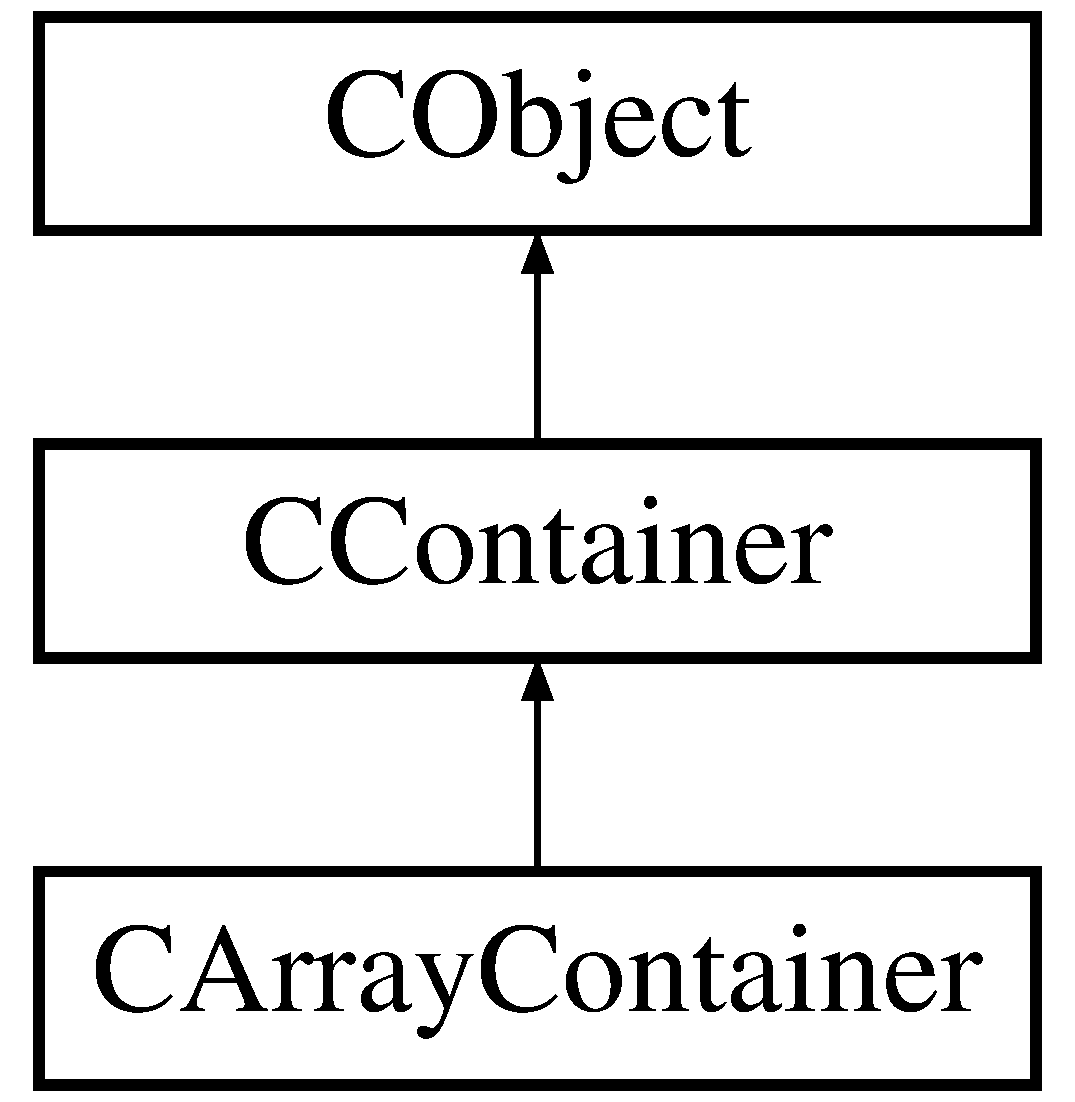
\includegraphics[height=3.000000cm]{class_c_array_container}
\end{center}
\end{figure}
\subsection*{Public Member Functions}
\begin{DoxyCompactItemize}
\item 
\hyperlink{class_c_array_container_a10e83176c2a2ee0d9fe53ca9e51b0ca0}{\-\_\-\-\_\-construct} (\$the\-Container=N\-U\-L\-L)
\item 
\hyperlink{class_c_array_container_ac63eeb55a8c374668c5c443fb6e27df3}{Container} (\$the\-Value=N\-U\-L\-L, \$get\-Old=F\-A\-L\-S\-E)
\item 
\hyperlink{class_c_array_container_ac89f1c53cc6680107cfb4703bd5103ca}{Commit} (\&\$the\-Object, \$the\-Identifier=N\-U\-L\-L, \$the\-Modifiers=k\-F\-L\-A\-G\-\_\-\-P\-E\-R\-S\-I\-S\-T\-\_\-\-R\-E\-P\-L\-A\-C\-E)
\end{DoxyCompactItemize}
\subsection*{Protected Member Functions}
\begin{DoxyCompactItemize}
\item 
\hyperlink{class_c_array_container_aed066fb29aae224fe77ce3d6e4540cac}{\-\_\-\-Commit} (\&\$the\-Object, \$the\-Identifier, \$the\-Modifiers)
\item 
\hyperlink{class_c_array_container_ac970cd81e09a1b87c6cad960de74856d}{\-\_\-\-Load} (\$the\-Identifier, \$the\-Modifiers)
\item 
\hyperlink{class_c_array_container_a7a6026166105a3d9281c3556836844bc}{\-\_\-\-Delete} (\$the\-Identifier, \$the\-Modifiers)
\end{DoxyCompactItemize}


\subsection{Constructor \& Destructor Documentation}
\hypertarget{class_c_array_container_a10e83176c2a2ee0d9fe53ca9e51b0ca0}{\index{C\-Array\-Container@{C\-Array\-Container}!\-\_\-\-\_\-construct@{\-\_\-\-\_\-construct}}
\index{\-\_\-\-\_\-construct@{\-\_\-\-\_\-construct}!CArrayContainer@{C\-Array\-Container}}
\subsubsection[{\-\_\-\-\_\-construct}]{\setlength{\rightskip}{0pt plus 5cm}{\bf C\-Array\-Container\-::\-\_\-\-\_\-construct} (
\begin{DoxyParamCaption}
\item[{\$}]{the\-Container = {\ttfamily NULL}}
\end{DoxyParamCaption}
)}}\label{class_c_array_container_a10e83176c2a2ee0d9fe53ca9e51b0ca0}
Instantiate class.

We \hyperlink{class_c_container_af2fc42b4d7b5f71e0f127c941440b1aa}{overload} this method to provide a default native container, which, in this case, will be an empty array.


\begin{DoxyParams}[1]{Parameters}
mixed & {\em \$the\-Container} & Native persistent container.\\
\hline
\end{DoxyParams}
public 

Reimplemented from \hyperlink{class_c_container_af2fc42b4d7b5f71e0f127c941440b1aa}{C\-Container}.



\subsection{Member Function Documentation}
\hypertarget{class_c_array_container_aed066fb29aae224fe77ce3d6e4540cac}{\index{C\-Array\-Container@{C\-Array\-Container}!\-\_\-\-Commit@{\-\_\-\-Commit}}
\index{\-\_\-\-Commit@{\-\_\-\-Commit}!CArrayContainer@{C\-Array\-Container}}
\subsubsection[{\-\_\-\-Commit}]{\setlength{\rightskip}{0pt plus 5cm}{\bf C\-Array\-Container\-::\-\_\-\-Commit} (
\begin{DoxyParamCaption}
\item[{\&\$}]{the\-Object, }
\item[{\$}]{the\-Identifier, }
\item[{\$}]{the\-Modifiers}
\end{DoxyParamCaption}
)\hspace{0.3cm}{\ttfamily  \mbox{[}protected\mbox{]}}}}\label{class_c_array_container_aed066fb29aae224fe77ce3d6e4540cac}
Commit provided object.

We implement this method to handle array or Array\-Object stores and we ensure provided options are followed.

By default the object must be an array or Array\-Object, any other type will raise an \hyperlink{}{exception}.

The provided identifier will be cast to a string. If it is {\itshape N\-U\-L\-L\/}, it means that the object is to be appended in the container and the method assumes the \hyperlink{class_c_array_container_ac89f1c53cc6680107cfb4703bd5103ca}{caller} has determined that it is an \hyperlink{}{insert} operation.

Although the \hyperlink{class_c_array_container_ac89f1c53cc6680107cfb4703bd5103ca}{caller} accepts the \hyperlink{}{delete} option, in this class we do not, so we shall raise an \hyperlink{}{exception}.


\begin{DoxyParams}[1]{Parameters}
reference & {\em \&\$the\-Object} & Object to commit. \\
\hline
mixed & {\em \$the\-Identifier} & Object identifier. \\
\hline
bitfield & {\em \$the\-Modifiers} & Commit modifiers.\\
\hline
\end{DoxyParams}
protected \begin{DoxyReturn}{Returns}
mixed 
\end{DoxyReturn}


Reimplemented from \hyperlink{class_c_container_a95c13ac30a01bd5ee684fe1baf0d8d43}{C\-Container}.

\hypertarget{class_c_array_container_a7a6026166105a3d9281c3556836844bc}{\index{C\-Array\-Container@{C\-Array\-Container}!\-\_\-\-Delete@{\-\_\-\-Delete}}
\index{\-\_\-\-Delete@{\-\_\-\-Delete}!CArrayContainer@{C\-Array\-Container}}
\subsubsection[{\-\_\-\-Delete}]{\setlength{\rightskip}{0pt plus 5cm}{\bf C\-Array\-Container\-::\-\_\-\-Delete} (
\begin{DoxyParamCaption}
\item[{\$}]{the\-Identifier, }
\item[{\$}]{the\-Modifiers}
\end{DoxyParamCaption}
)\hspace{0.3cm}{\ttfamily  \mbox{[}protected\mbox{]}}}}\label{class_c_array_container_a7a6026166105a3d9281c3556836844bc}
Delete object.

We implement this method to handle array or Array\-Object stores.

The method will cast the identifier to a string.


\begin{DoxyParams}[1]{Parameters}
mixed & {\em \$the\-Identifier} & Object identifier. \\
\hline
bitfield & {\em \$the\-Modifiers} & Load modifiers.\\
\hline
\end{DoxyParams}
protected \begin{DoxyReturn}{Returns}
mixed 
\end{DoxyReturn}


Reimplemented from \hyperlink{class_c_container_adb859efe2ce642d29d3bff48a806789d}{C\-Container}.

\hypertarget{class_c_array_container_ac970cd81e09a1b87c6cad960de74856d}{\index{C\-Array\-Container@{C\-Array\-Container}!\-\_\-\-Load@{\-\_\-\-Load}}
\index{\-\_\-\-Load@{\-\_\-\-Load}!CArrayContainer@{C\-Array\-Container}}
\subsubsection[{\-\_\-\-Load}]{\setlength{\rightskip}{0pt plus 5cm}{\bf C\-Array\-Container\-::\-\_\-\-Load} (
\begin{DoxyParamCaption}
\item[{\$}]{the\-Identifier, }
\item[{\$}]{the\-Modifiers}
\end{DoxyParamCaption}
)\hspace{0.3cm}{\ttfamily  \mbox{[}protected\mbox{]}}}}\label{class_c_array_container_ac970cd81e09a1b87c6cad960de74856d}
Load object.

We implement this method to handle array or Array\-Object stores.

The method will cast the identifier to a string.


\begin{DoxyParams}[1]{Parameters}
mixed & {\em \$the\-Identifier} & Object identifier. \\
\hline
bitfield & {\em \$the\-Modifiers} & Load modifiers.\\
\hline
\end{DoxyParams}
protected \begin{DoxyReturn}{Returns}
mixed 
\end{DoxyReturn}


Reimplemented from \hyperlink{class_c_container_a93d34640379c1debc9542609bf4b34e9}{C\-Container}.

\hypertarget{class_c_array_container_ac89f1c53cc6680107cfb4703bd5103ca}{\index{C\-Array\-Container@{C\-Array\-Container}!Commit@{Commit}}
\index{Commit@{Commit}!CArrayContainer@{C\-Array\-Container}}
\subsubsection[{Commit}]{\setlength{\rightskip}{0pt plus 5cm}{\bf C\-Array\-Container\-::\-Commit} (
\begin{DoxyParamCaption}
\item[{\&\$}]{the\-Object, }
\item[{\$}]{the\-Identifier = {\ttfamily NULL}, }
\item[{\$}]{the\-Modifiers = {\ttfamily kFLAG\-\_\-PERSIST\-\_\-REPLACE}}
\end{DoxyParamCaption}
)}}\label{class_c_array_container_ac89f1c53cc6680107cfb4703bd5103ca}
Commit provided object.

We \hyperlink{class_c_container_a4847dc676d1f7704e75f8981e927508a}{overload} this method to check whether the provided object is either an array or an Array\-Object.


\begin{DoxyParams}[1]{Parameters}
reference & {\em \&\$the\-Object} & Object to commit. \\
\hline
mixed & {\em \$the\-Identifier} & Object identifier. \\
\hline
bitfield & {\em \$the\-Modifiers} & Commit modifiers.\\
\hline
\end{DoxyParams}
public \begin{DoxyReturn}{Returns}
mixed 
\end{DoxyReturn}


Reimplemented from \hyperlink{class_c_container_a4847dc676d1f7704e75f8981e927508a}{C\-Container}.

\hypertarget{class_c_array_container_ac63eeb55a8c374668c5c443fb6e27df3}{\index{C\-Array\-Container@{C\-Array\-Container}!Container@{Container}}
\index{Container@{Container}!CArrayContainer@{C\-Array\-Container}}
\subsubsection[{Container}]{\setlength{\rightskip}{0pt plus 5cm}{\bf C\-Array\-Container\-::\-Container} (
\begin{DoxyParamCaption}
\item[{\$}]{the\-Value = {\ttfamily NULL}, }
\item[{\$}]{get\-Old = {\ttfamily FALSE}}
\end{DoxyParamCaption}
)}}\label{class_c_array_container_ac63eeb55a8c374668c5c443fb6e27df3}
Manage persistent container.

We \hyperlink{class_c_container_a7d10fa70dfa381cb95e66c265e2ca113}{overload} this method to ensure that the provided container is either an array or an Array\-Object.


\begin{DoxyParams}[1]{Parameters}
mixed & {\em \$the\-Value} & Persistent container or operation. \\
\hline
boolean & {\em \$get\-Old} & T\-R\-U\-E get old value.\\
\hline
\end{DoxyParams}
public \begin{DoxyReturn}{Returns}
mixed
\end{DoxyReturn}
\hyperlink{class_c_object_a9b8dccdadcf4fea58f915bd9b228e23e}{Manage\-Member()} 

Reimplemented from \hyperlink{class_c_container_a7d10fa70dfa381cb95e66c265e2ca113}{C\-Container}.



The documentation for this class was generated from the following file\-:\begin{DoxyCompactItemize}
\item 
/\-Library/\-Web\-Server/\-Library/wrapper/classes/C\-Array\-Container.\-php\end{DoxyCompactItemize}

\hypertarget{class_c_array_object}{\section{C\-Array\-Object Class Reference}
\label{class_c_array_object}\index{C\-Array\-Object@{C\-Array\-Object}}
}
Inheritance diagram for C\-Array\-Object\-:\begin{figure}[H]
\begin{center}
\leavevmode
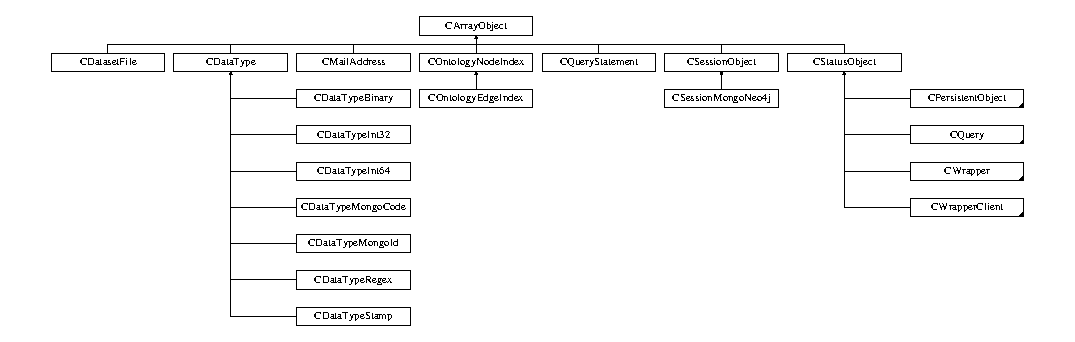
\includegraphics[height=5.874125cm]{class_c_array_object}
\end{center}
\end{figure}
\subsection*{Public Member Functions}
\begin{DoxyCompactItemize}
\item 
\hyperlink{class_c_array_object_ac9929feeb67c76a0e055696abffe2fb6}{offset\-Get} (\$the\-Offset)
\item 
\hyperlink{class_c_array_object_a41815b543b14d373f68ed34ca53dc9f6}{offset\-Set} (\$the\-Offset, \$the\-Value)
\item 
\hyperlink{class_c_array_object_a2852b78f58379e507b5e7d7cb8e5326b}{offset\-Unset} (\$the\-Offset)
\item 
\hyperlink{class_c_array_object_a350d95184af98e75868f27ea170270ce}{keys} ()
\item 
\hyperlink{class_c_array_object_a1f29fcc343a624354f6096fd6a4621e6}{values} ()
\end{DoxyCompactItemize}
\subsection*{Protected Member Functions}
\begin{DoxyCompactItemize}
\item 
\hyperlink{class_c_array_object_a931cb8b30569b811a18adc0161eb3603}{\-\_\-\-Manage\-Offset} (\$the\-Offset, \$the\-Value=N\-U\-L\-L, \$get\-Old=F\-A\-L\-S\-E)
\item 
\hyperlink{class_c_array_object_a056b7a3218ffb9a2eb992c029124a669}{\-\_\-\-Manage\-Array\-Offset} (\$the\-Offset, \$the\-Value=N\-U\-L\-L, \$the\-Operation=N\-U\-L\-L, \$get\-Old=F\-A\-L\-S\-E)
\item 
\hyperlink{class_c_array_object_af714f81bb75f725c6868fb286c59b160}{\-\_\-\-Manage\-Typed\-Array\-Offset} (\$the\-Offset, \$the\-Type=N\-U\-L\-L, \$the\-Data=N\-U\-L\-L, \$get\-Old=F\-A\-L\-S\-E)
\end{DoxyCompactItemize}


\subsection{Member Function Documentation}
\hypertarget{class_c_array_object_a056b7a3218ffb9a2eb992c029124a669}{\index{C\-Array\-Object@{C\-Array\-Object}!\-\_\-\-Manage\-Array\-Offset@{\-\_\-\-Manage\-Array\-Offset}}
\index{\-\_\-\-Manage\-Array\-Offset@{\-\_\-\-Manage\-Array\-Offset}!CArrayObject@{C\-Array\-Object}}
\subsubsection[{\-\_\-\-Manage\-Array\-Offset}]{\setlength{\rightskip}{0pt plus 5cm}{\bf C\-Array\-Object\-::\-\_\-\-Manage\-Array\-Offset} (
\begin{DoxyParamCaption}
\item[{\$}]{the\-Offset, }
\item[{\$}]{the\-Value = {\ttfamily NULL}, }
\item[{\$}]{the\-Operation = {\ttfamily NULL}, }
\item[{\$}]{get\-Old = {\ttfamily FALSE}}
\end{DoxyParamCaption}
)\hspace{0.3cm}{\ttfamily  \mbox{[}protected\mbox{]}}}}\label{class_c_array_object_a056b7a3218ffb9a2eb992c029124a669}
Manage an array offset.

This library implements a standard interface for managing object properties using methods, this method extends the approach to offset members that are in the form of arrays, in which it should be possible to cast the values to strings and these strings should be unique within the list\-:


\begin{DoxyItemize}
\item {\bfseries \$the\-Offset}\-: The offset to manage. 
\item {\bfseries \$the\-Value}\-: This parameter represents either the value to add, or the index of the element to operate on\-: 
\begin{DoxyItemize}
\item {\itshape N\-U\-L\-L\/}\-: This value indicates that we want to operate on all elements, which means that we are either retrieving the full list or deleting it. 
\item {\itshape array\/}\-: This value indicates that we want to replace the whole list, this will only be tested if the next parameter evaluates to {\itshape T\-R\-U\-E\/}. 
\item {\itshape other\/}\-: Any other type represents either the new value to be added or the index to the value to be returned or deleted. {\itshape It must be possible to cast this value to a string, this is what will be used to compare elements\/}. 
\end{DoxyItemize}
\item {\bfseries \$the\-Operation}\-: This parameter represents the operation to be performed, it will be evaluated as a boolean and its scope depends on the value of the previous parameter\-: 
\begin{DoxyItemize}
\item {\itshape N\-U\-L\-L\/}\-: Return the element or list. 
\item {\itshape F\-A\-L\-S\-E\/}\-: Delete the element or list. 
\item {\itshape T\-R\-U\-E\/}\-: Add the element or list. Note that with this value, if you provide {\itshape N\-U\-L\-L\/} in the previous parameter, it will be equivalent to deleting the whole list. 
\end{DoxyItemize}
\item {\bfseries \$get\-Old}\-: Determines what the method will return\-: 
\begin{DoxyItemize}
\item {\itshape T\-R\-U\-E\/}\-: Return the element or list {\itshape before\/} it was eventually modified. 
\item {\itshape F\-A\-L\-S\-E\/}\-: Return the element or list {\itshape after\/} it was eventually modified. 
\end{DoxyItemize}
\end{DoxyItemize}


\begin{DoxyParams}[1]{Parameters}
string & {\em \$the\-Offset} & Offset. \\
\hline
mixed & {\em \$the\-Value} & Value or index. \\
\hline
mixed & {\em \$the\-Operation} & Operation. \\
\hline
boolean & {\em \$get\-Old} & T\-R\-U\-E get old value.\\
\hline
\end{DoxyParams}
protected \begin{DoxyReturn}{Returns}
mixed
\end{DoxyReturn}
\hyperlink{class_c_array_object_ac9929feeb67c76a0e055696abffe2fb6}{offset\-Get()}  \hyperlink{class_c_array_object_a41815b543b14d373f68ed34ca53dc9f6}{offset\-Set()}  \hyperlink{class_c_array_object_a2852b78f58379e507b5e7d7cb8e5326b}{offset\-Unset()} \hypertarget{class_c_array_object_a931cb8b30569b811a18adc0161eb3603}{\index{C\-Array\-Object@{C\-Array\-Object}!\-\_\-\-Manage\-Offset@{\-\_\-\-Manage\-Offset}}
\index{\-\_\-\-Manage\-Offset@{\-\_\-\-Manage\-Offset}!CArrayObject@{C\-Array\-Object}}
\subsubsection[{\-\_\-\-Manage\-Offset}]{\setlength{\rightskip}{0pt plus 5cm}{\bf C\-Array\-Object\-::\-\_\-\-Manage\-Offset} (
\begin{DoxyParamCaption}
\item[{\$}]{the\-Offset, }
\item[{\$}]{the\-Value = {\ttfamily NULL}, }
\item[{\$}]{get\-Old = {\ttfamily FALSE}}
\end{DoxyParamCaption}
)\hspace{0.3cm}{\ttfamily  \mbox{[}protected\mbox{]}}}}\label{class_c_array_object_a931cb8b30569b811a18adc0161eb3603}
Manage an offset.

This library implements a standard interface for managing object properties using methods, this method extends the approach to offset members\-:


\begin{DoxyItemize}
\item {\bfseries \$the\-Offset}\-: The offset to manage. 
\item {\bfseries \$the\-Value}\-: The value or operation\-: 
\begin{DoxyItemize}
\item {\itshape N\-U\-L\-L\/}\-: Return the offset's current value. 
\item {\itshape F\-A\-L\-S\-E\/}\-: Delete the offset. 
\item {\itshape other\/}\-: Any other type represents the offset's new value. 
\end{DoxyItemize}
\item {\bfseries \$get\-Old}\-: Determines what the method will return\-: 
\begin{DoxyItemize}
\item {\itshape T\-R\-U\-E\/}\-: Return the value of the offset {\itshape before\/} it was eventually modified. 
\item {\itshape F\-A\-L\-S\-E\/}\-: Return the value of the offset {\itshape after\/} it was eventually modified. 
\end{DoxyItemize}
\end{DoxyItemize}


\begin{DoxyParams}[1]{Parameters}
string & {\em \$the\-Offset} & Offset. \\
\hline
mixed & {\em \$the\-Value} & Value or operation. \\
\hline
boolean & {\em \$get\-Old} & T\-R\-U\-E get old value.\\
\hline
\end{DoxyParams}
protected \begin{DoxyReturn}{Returns}
mixed
\end{DoxyReturn}
\hyperlink{class_c_array_object_ac9929feeb67c76a0e055696abffe2fb6}{offset\-Get()}  \hyperlink{class_c_array_object_a41815b543b14d373f68ed34ca53dc9f6}{offset\-Set()}  \hyperlink{class_c_array_object_a2852b78f58379e507b5e7d7cb8e5326b}{offset\-Unset()} \hypertarget{class_c_array_object_af714f81bb75f725c6868fb286c59b160}{\index{C\-Array\-Object@{C\-Array\-Object}!\-\_\-\-Manage\-Typed\-Array\-Offset@{\-\_\-\-Manage\-Typed\-Array\-Offset}}
\index{\-\_\-\-Manage\-Typed\-Array\-Offset@{\-\_\-\-Manage\-Typed\-Array\-Offset}!CArrayObject@{C\-Array\-Object}}
\subsubsection[{\-\_\-\-Manage\-Typed\-Array\-Offset}]{\setlength{\rightskip}{0pt plus 5cm}{\bf C\-Array\-Object\-::\-\_\-\-Manage\-Typed\-Array\-Offset} (
\begin{DoxyParamCaption}
\item[{\$}]{the\-Offset, }
\item[{\$}]{the\-Type = {\ttfamily NULL}, }
\item[{\$}]{the\-Data = {\ttfamily NULL}, }
\item[{\$}]{get\-Old = {\ttfamily FALSE}}
\end{DoxyParamCaption}
)\hspace{0.3cm}{\ttfamily  \mbox{[}protected\mbox{]}}}}\label{class_c_array_object_af714f81bb75f725c6868fb286c59b160}
Manage a typed array offset.

This library implements a standard interface for managing object properties using methods, this method extends the approach to offset members that are in the form of arrays, in which each element is itself an array of two items\-:


\begin{DoxyItemize}
\item {\itshape \hyperlink{}{k\-T\-A\-G\-\_\-\-T\-Y\-P\-E}\/}\-: This element represents the qualifier of the item, it provides a type or qualification for the next element. It must be possible to cast this value to a string. 
\item {\itshape \hyperlink{}{k\-T\-A\-G\-\_\-\-D\-A\-T\-A}\/}\-: This element represents the element data. 
\end{DoxyItemize}

No two elements of the list can share the same \hyperlink{}{type}. You may have one element without \hyperlink{}{type}, this one may be considered the default element.

This method is intended for managing list elements rather than the list itself, for the latter purpose use the offset management methods.

The parameters to this method are\-:


\begin{DoxyItemize}
\item {\bfseries \$the\-Offset}\-: The offset to manage. 
\item {\bfseries \$the\-Type}\-: This parameter represents the value of the \hyperlink{}{type} element of the item, depending on the next parameter this value will be used for matching items in the list\-: 
\begin{DoxyItemize}
\item {\itshape N\-U\-L\-L\/}\-: An empty type means that we are looking for the item lacking the \hyperlink{}{k\-T\-A\-G\-\_\-\-T\-Y\-P\-E} tag. 
\item {\itshape array\/}\-: If you provide an array, it means that you are operating on a list of items\-: depending on the next parameter this will mean either retrieving the \hyperlink{}{data} elements of the items matching the array, deleting these items, or adding/replacing the items; in this last case, this means that the next parameter must also be an array and that each of its elements will be associated to the corresponding \hyperlink{}{type} element. 
\item {\itshape other\/}\-: Any other value will be considered as the type to retrieve, remove or add/replace. You {\itshape M\-U\-S\-T\/} be able to cast this value to a string. 
\end{DoxyItemize}
\item {\bfseries \$the\-Data}\-: This parameter represents the item's \hyperlink{}{data} element, or the operation to be performed\-: 
\begin{DoxyItemize}
\item {\itshape N\-U\-L\-L\/}\-: This indicates that we want to retrieve the data of the item with \hyperlink{}{type} matching the previous parameter. 
\item {\itshape F\-A\-L\-S\-E\/}\-: This indicates that we want to remove the item matching the \hyperlink{}{type} provided in the previous parameter. 
\item {\itshape other\/}\-: Any other value indicates that we want to add or replace the \hyperlink{}{data} element of the item matching the previous parameter. Note that if the previous parameter is an array, this one must also be an array matching the latter's count. 
\end{DoxyItemize}
\item {\bfseries \$get\-Old}\-: Determines what the method will return\-: 
\begin{DoxyItemize}
\item {\itshape T\-R\-U\-E\/}\-: Return the element or list {\itshape before\/} it was eventually modified. 
\item {\itshape F\-A\-L\-S\-E\/}\-: Return the element or list {\itshape after\/} it was eventually modified. 
\end{DoxyItemize}
\end{DoxyItemize}


\begin{DoxyParams}[1]{Parameters}
string & {\em \$the\-Offset} & Offset. \\
\hline
mixed & {\em \$the\-Type} & Element type. \\
\hline
mixed & {\em \$the\-Data} & Element value. \\
\hline
boolean & {\em \$get\-Old} & T\-R\-U\-E get old value.\\
\hline
\end{DoxyParams}
protected \begin{DoxyReturn}{Returns}
mixed
\end{DoxyReturn}
\hyperlink{class_c_array_object_ac9929feeb67c76a0e055696abffe2fb6}{offset\-Get()}  \hyperlink{class_c_array_object_a41815b543b14d373f68ed34ca53dc9f6}{offset\-Set()}  \hyperlink{class_c_array_object_a2852b78f58379e507b5e7d7cb8e5326b}{offset\-Unset()} \hypertarget{class_c_array_object_a350d95184af98e75868f27ea170270ce}{\index{C\-Array\-Object@{C\-Array\-Object}!keys@{keys}}
\index{keys@{keys}!CArrayObject@{C\-Array\-Object}}
\subsubsection[{keys}]{\setlength{\rightskip}{0pt plus 5cm}{\bf C\-Array\-Object\-::keys} (
\begin{DoxyParamCaption}
{}
\end{DoxyParamCaption}
)}}\label{class_c_array_object_a350d95184af98e75868f27ea170270ce}
Return object's keys.

This method has the same function as array's {\itshape array\-\_\-keys()\/}, it will return an array comprised of all object's offsets.

public \begin{DoxyReturn}{Returns}
array 
\end{DoxyReturn}
\hypertarget{class_c_array_object_ac9929feeb67c76a0e055696abffe2fb6}{\index{C\-Array\-Object@{C\-Array\-Object}!offset\-Get@{offset\-Get}}
\index{offset\-Get@{offset\-Get}!CArrayObject@{C\-Array\-Object}}
\subsubsection[{offset\-Get}]{\setlength{\rightskip}{0pt plus 5cm}{\bf C\-Array\-Object\-::offset\-Get} (
\begin{DoxyParamCaption}
\item[{\$}]{the\-Offset}
\end{DoxyParamCaption}
)}}\label{class_c_array_object_ac9929feeb67c76a0e055696abffe2fb6}
Return a value at a given offset.

This method should return the value corresponding to the provided offset.

This method is overloaded to prevent notices from being triggered when seeking non-\/existing offsets.

In this class no offset may have a {\itshape N\-U\-L\-L\/} value, if this method returns a {\itshape N\-U\-L\-L\/} value, it means that the offset doesn't exist.


\begin{DoxyParams}[1]{Parameters}
string & {\em \$the\-Offset} & Offset.\\
\hline
\end{DoxyParams}
public \begin{DoxyReturn}{Returns}
mixed 
\end{DoxyReturn}
\hypertarget{class_c_array_object_a41815b543b14d373f68ed34ca53dc9f6}{\index{C\-Array\-Object@{C\-Array\-Object}!offset\-Set@{offset\-Set}}
\index{offset\-Set@{offset\-Set}!CArrayObject@{C\-Array\-Object}}
\subsubsection[{offset\-Set}]{\setlength{\rightskip}{0pt plus 5cm}{\bf C\-Array\-Object\-::offset\-Set} (
\begin{DoxyParamCaption}
\item[{\$}]{the\-Offset, }
\item[{\$}]{the\-Value}
\end{DoxyParamCaption}
)}}\label{class_c_array_object_a41815b543b14d373f68ed34ca53dc9f6}
Set a value for a given offset.

This method should set the provided value corresponding to the provided offset.

This method is overloaded to prevent setting {\itshape N\-U\-L\-L\/} values\-: if this is the case, the method will \hyperlink{class_c_array_object_a2852b78f58379e507b5e7d7cb8e5326b}{delete} the offset.


\begin{DoxyParams}[1]{Parameters}
string & {\em \$the\-Offset} & Offset. \\
\hline
string | N\-U\-L\-L & {\em \$the\-Value} & Value to set at offset.\\
\hline
\end{DoxyParams}
public

\hyperlink{class_c_array_object_a2852b78f58379e507b5e7d7cb8e5326b}{offset\-Unset()} 

Reimplemented in \hyperlink{class_c_entity_a193cf3d19057021bb6e779644730eac8}{C\-Entity}, \hyperlink{class_c_user_aace3446b9cacfe28cc1937c608fcc999}{C\-User}, and \hyperlink{class_c_status_object_a140ef140d4fa1c4a6180e843bd5ec969}{C\-Status\-Object}.

\hypertarget{class_c_array_object_a2852b78f58379e507b5e7d7cb8e5326b}{\index{C\-Array\-Object@{C\-Array\-Object}!offset\-Unset@{offset\-Unset}}
\index{offset\-Unset@{offset\-Unset}!CArrayObject@{C\-Array\-Object}}
\subsubsection[{offset\-Unset}]{\setlength{\rightskip}{0pt plus 5cm}{\bf C\-Array\-Object\-::offset\-Unset} (
\begin{DoxyParamCaption}
\item[{\$}]{the\-Offset}
\end{DoxyParamCaption}
)}}\label{class_c_array_object_a2852b78f58379e507b5e7d7cb8e5326b}
Reset a value for a given offset.

This method should reset the value corresponding to the provided offset.

We overload this method to prevent notices on non-\/existing offsets.


\begin{DoxyParams}[1]{Parameters}
string & {\em \$the\-Offset} & Offset.\\
\hline
\end{DoxyParams}
public 

Reimplemented in \hyperlink{class_c_entity_a887a87fc716e36a0d4c1477dbaf5bb67}{C\-Entity}, \hyperlink{class_c_user_aed8557e18a89d868cedf5a48328b33b2}{C\-User}, and \hyperlink{class_c_status_object_ae733db1bbfffcbe894ea405765ab4150}{C\-Status\-Object}.

\hypertarget{class_c_array_object_a1f29fcc343a624354f6096fd6a4621e6}{\index{C\-Array\-Object@{C\-Array\-Object}!values@{values}}
\index{values@{values}!CArrayObject@{C\-Array\-Object}}
\subsubsection[{values}]{\setlength{\rightskip}{0pt plus 5cm}{\bf C\-Array\-Object\-::values} (
\begin{DoxyParamCaption}
{}
\end{DoxyParamCaption}
)}}\label{class_c_array_object_a1f29fcc343a624354f6096fd6a4621e6}
Return object's values.

This method has the same function as array's {\itshape array\-\_\-values()\/}, it will return an array comprised of all object's values.

public \begin{DoxyReturn}{Returns}
array 
\end{DoxyReturn}


The documentation for this class was generated from the following file\-:\begin{DoxyCompactItemize}
\item 
/\-Library/\-Web\-Server/\-Library/wrapper/classes/C\-Array\-Object.\-php\end{DoxyCompactItemize}

\hypertarget{class_c_container}{\section{C\-Container Class Reference}
\label{class_c_container}\index{C\-Container@{C\-Container}}
}
Inheritance diagram for C\-Container\-:\begin{figure}[H]
\begin{center}
\leavevmode
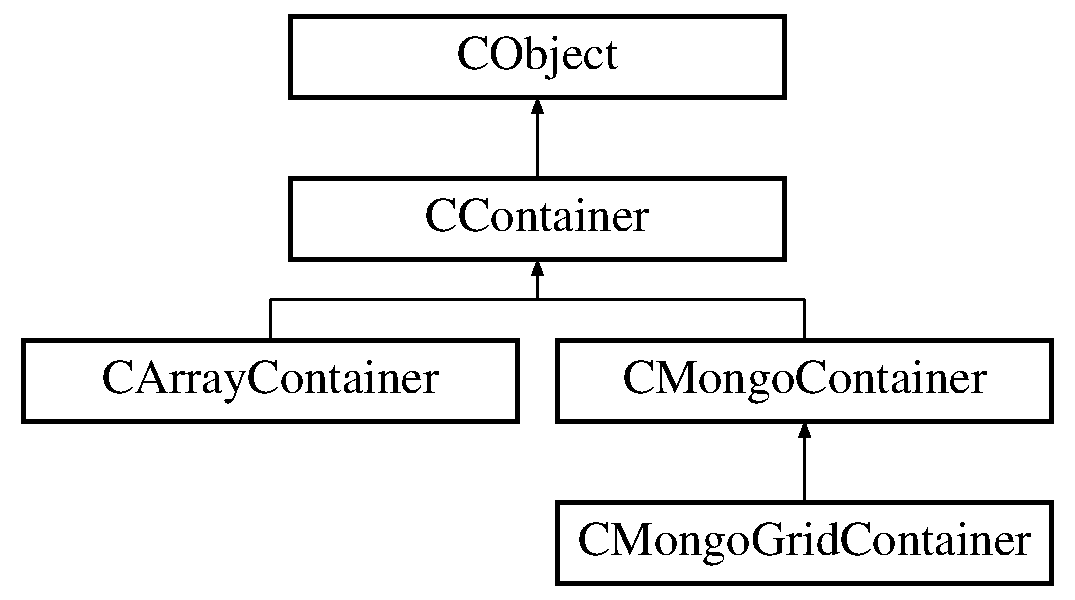
\includegraphics[height=4.000000cm]{class_c_container}
\end{center}
\end{figure}
\subsection*{Public Member Functions}
\begin{DoxyCompactItemize}
\item 
\hyperlink{class_c_container_af2fc42b4d7b5f71e0f127c941440b1aa}{\-\_\-\-\_\-construct} (\$the\-Container=N\-U\-L\-L)
\item 
\hyperlink{class_c_container_aa1d6ed5052f55cdffcf6445968f203ed}{\-\_\-\-\_\-to\-String} ()
\item 
\hyperlink{class_c_container_a7d10fa70dfa381cb95e66c265e2ca113}{Container} (\$the\-Value=N\-U\-L\-L, \$get\-Old=F\-A\-L\-S\-E)
\item 
\hyperlink{class_c_container_a0d691b62d9b70b924e24a332931ce9d1}{Database} ()
\item 
\hyperlink{class_c_container_a4847dc676d1f7704e75f8981e927508a}{Commit} (\&\$the\-Object, \$the\-Identifier=N\-U\-L\-L, \$the\-Modifiers=k\-F\-L\-A\-G\-\_\-\-P\-E\-R\-S\-I\-S\-T\-\_\-\-R\-E\-P\-L\-A\-C\-E)
\item 
\hyperlink{class_c_container_a48db96aa6bbf15d0bfc15725616b7154}{Load} (\$the\-Identifier, \$the\-Modifiers=k\-F\-L\-A\-G\-\_\-\-D\-E\-F\-A\-U\-L\-T)
\item 
\hyperlink{class_c_container_aa91ec2f4624a2ebfb74668f274139329}{Delete} (\$the\-Identifier, \$the\-Modifiers=k\-F\-L\-A\-G\-\_\-\-D\-E\-F\-A\-U\-L\-T)
\item 
\hyperlink{class_c_container_a1486a3cb34d24ff1c3028ad4360b5dc6}{Reference} (\$the\-Object, \$the\-Modifiers=k\-F\-L\-A\-G\-\_\-\-R\-E\-F\-E\-R\-E\-N\-C\-E\-\_\-\-I\-D\-E\-N\-T\-I\-F\-I\-E\-R)
\item 
\hyperlink{class_c_container_aa339d3c4c9b011713176a89fe9c7783d}{Unserialise\-Object} (\&\$the\-Object)
\item 
\hyperlink{class_c_container_a09d585e2a9809221a42d52d7520c9cbf}{Unserialise\-Data} (\&\$the\-Element)
\end{DoxyCompactItemize}
\subsection*{Protected Member Functions}
\begin{DoxyCompactItemize}
\item 
\& \hyperlink{class_c_container_a4794d326f4ffd3c2b8afd2e0460604ff}{\-\_\-\-Container} ()
\item 
\hyperlink{class_c_container_acbc85dd164615b31c9edfec93bcf27f9}{\-\_\-\-Commit} (\&\$the\-Object, \&\$the\-Identifier, \&\$the\-Modifiers)
\item 
\hyperlink{class_c_container_a865f140560991fa21a88b7fc8ff8f1f5}{\-\_\-\-Load} (\&\$the\-Identifier, \&\$the\-Modifiers)
\item 
\hyperlink{class_c_container_a20aac3eec154c2122f2c602bf5ce35fe}{\-\_\-\-Delete} (\&\$the\-Identifier, \&\$the\-Modifiers)
\item 
\hyperlink{class_c_container_a0dc47e54abc533cedf1c2c0f915d96b2}{\-\_\-\-Prepare\-Commit} (\&\$the\-Object, \&\$the\-Identifier, \&\$the\-Modifiers)
\item 
\hyperlink{class_c_container_a1b84868c32fcfd3e11a9f6cc85fc461c}{\-\_\-\-Prepare\-Load} (\&\$the\-Identifier, \&\$the\-Modifiers)
\item 
\hyperlink{class_c_container_a238776ec6152dd400be2ed87ba949fd0}{\-\_\-\-Prepare\-Delete} (\&\$the\-Identifier, \&\$the\-Modifiers)
\item 
\hyperlink{class_c_container_a4c9cae709a81dd53c7307bfbde891fae}{\-\_\-\-Finish\-Commit} (\&\$the\-Object, \&\$the\-Identifier, \&\$the\-Modifiers)
\item 
\hyperlink{class_c_container_ab53bd683f0e28b2203897cf03f9d1c76}{\-\_\-\-Finish\-Load} (\&\$the\-Object, \&\$the\-Identifier, \&\$the\-Modifiers)
\item 
\hyperlink{class_c_container_ab8bfc9866573dd474dcf418059d94fbe}{\-\_\-\-Finish\-Delete} (\&\$the\-Object, \&\$the\-Identifier, \&\$the\-Modifiers)
\end{DoxyCompactItemize}
\subsection*{Protected Attributes}
\begin{DoxyCompactItemize}
\item 
\hypertarget{class_c_container_a52a8e4284fff9530c1ff25c93b238b9f}{{\bfseries \$m\-Container} = N\-U\-L\-L}\label{class_c_container_a52a8e4284fff9530c1ff25c93b238b9f}

\end{DoxyCompactItemize}
\subsection*{Additional Inherited Members}


\subsection{Constructor \& Destructor Documentation}
\hypertarget{class_c_container_af2fc42b4d7b5f71e0f127c941440b1aa}{\index{C\-Container@{C\-Container}!\-\_\-\-\_\-construct@{\-\_\-\-\_\-construct}}
\index{\-\_\-\-\_\-construct@{\-\_\-\-\_\-construct}!CContainer@{C\-Container}}
\subsubsection[{\-\_\-\-\_\-construct}]{\setlength{\rightskip}{0pt plus 5cm}C\-Container\-::\-\_\-\-\_\-construct (
\begin{DoxyParamCaption}
\item[{}]{\$the\-Container = {\ttfamily NULL}}
\end{DoxyParamCaption}
)}}\label{class_c_container_af2fc42b4d7b5f71e0f127c941440b1aa}
Instantiate class.

You instantiate the class with a native data store, the method expects a single parameter that will be handled specifically by specialised derived classes.

Derived classes should overload this method if a default value is possible; to check for specific container types they should rather overload the member accessor \hyperlink{class_c_container_a7d10fa70dfa381cb95e66c265e2ca113}{method}.


\begin{DoxyParams}[1]{Parameters}
mixed & {\em \$the\-Container} & Native object store.\\
\hline
\end{DoxyParams}
public

\hyperlink{class_c_container_a7d10fa70dfa381cb95e66c265e2ca113}{Container()} 

Reimplemented in \hyperlink{class_c_array_container_a10e83176c2a2ee0d9fe53ca9e51b0ca0}{C\-Array\-Container}.



\subsection{Member Function Documentation}
\hypertarget{class_c_container_aa1d6ed5052f55cdffcf6445968f203ed}{\index{C\-Container@{C\-Container}!\-\_\-\-\_\-to\-String@{\-\_\-\-\_\-to\-String}}
\index{\-\_\-\-\_\-to\-String@{\-\_\-\-\_\-to\-String}!CContainer@{C\-Container}}
\subsubsection[{\-\_\-\-\_\-to\-String}]{\setlength{\rightskip}{0pt plus 5cm}C\-Container\-::\-\_\-\-\_\-to\-String (
\begin{DoxyParamCaption}
{}
\end{DoxyParamCaption}
)\hspace{0.3cm}{\ttfamily [abstract]}}}\label{class_c_container_aa1d6ed5052f55cdffcf6445968f203ed}
Return container name.

This method should return the current container's name.

All derived concrete classes should implement this method, all containers must be able to return a name.

public \begin{DoxyReturn}{Returns}
string 
\end{DoxyReturn}


Reimplemented in \hyperlink{class_c_array_container_aa7739e1def0a13a6750d6fa722952bcc}{C\-Array\-Container}, and \hyperlink{class_c_mongo_container_abc325eae251667da577efdb45a7d3c17}{C\-Mongo\-Container}.

\hypertarget{class_c_container_acbc85dd164615b31c9edfec93bcf27f9}{\index{C\-Container@{C\-Container}!\-\_\-\-Commit@{\-\_\-\-Commit}}
\index{\-\_\-\-Commit@{\-\_\-\-Commit}!CContainer@{C\-Container}}
\subsubsection[{\-\_\-\-Commit}]{\setlength{\rightskip}{0pt plus 5cm}C\-Container\-::\-\_\-\-Commit (
\begin{DoxyParamCaption}
\item[{\&}]{\$the\-Object, }
\item[{\&}]{\$the\-Identifier, }
\item[{\&}]{\$the\-Modifiers}
\end{DoxyParamCaption}
)\hspace{0.3cm}{\ttfamily [abstract]}, {\ttfamily [protected]}}}\label{class_c_container_acbc85dd164615b31c9edfec93bcf27f9}
Commit provided object.

Derived classes must implement this method to actually store the provided object in the container, the method expects the same parameters as the public \hyperlink{class_c_container_a4847dc676d1f7704e75f8981e927508a}{interface}, except that in this method these are passed by reference.

The method should return the object's key within the container or raise an exception if the operation was not successful.


\begin{DoxyParams}[1]{Parameters}
reference & {\em \&\$the\-Object} & Object to commit. \\
\hline
reference & {\em \&\$the\-Identifier} & Object identifier. \\
\hline
reference & {\em \&\$the\-Modifiers} & Commit modifiers.\\
\hline
\end{DoxyParams}
protected \begin{DoxyReturn}{Returns}
mixed 
\end{DoxyReturn}


Reimplemented in \hyperlink{class_c_mongo_container_a92cbcdba4f2b0bda2ae3eeb7a08d7ba2}{C\-Mongo\-Container}, \hyperlink{class_c_array_container_a8f58eaea0751d43e4ac7a5d4c732ddaa}{C\-Array\-Container}, and \hyperlink{class_c_mongo_grid_container_a1dc8378e77df7c06afc2c733e2422482}{C\-Mongo\-Grid\-Container}.

\hypertarget{class_c_container_a4794d326f4ffd3c2b8afd2e0460604ff}{\index{C\-Container@{C\-Container}!\-\_\-\-Container@{\-\_\-\-Container}}
\index{\-\_\-\-Container@{\-\_\-\-Container}!CContainer@{C\-Container}}
\subsubsection[{\-\_\-\-Container}]{\setlength{\rightskip}{0pt plus 5cm}\& C\-Container\-::\-\_\-\-Container (
\begin{DoxyParamCaption}
{}
\end{DoxyParamCaption}
)\hspace{0.3cm}{\ttfamily [protected]}}}\label{class_c_container_a4794d326f4ffd3c2b8afd2e0460604ff}
Get container reference.

This method can be used to retrieve a reference to the native container member, this can be useful when the native \hyperlink{class_c_container_a7d10fa70dfa381cb95e66c265e2ca113}{container} is not an object passed by reference.

protected \begin{DoxyReturn}{Returns}
mixed 
\end{DoxyReturn}
\hypertarget{class_c_container_a20aac3eec154c2122f2c602bf5ce35fe}{\index{C\-Container@{C\-Container}!\-\_\-\-Delete@{\-\_\-\-Delete}}
\index{\-\_\-\-Delete@{\-\_\-\-Delete}!CContainer@{C\-Container}}
\subsubsection[{\-\_\-\-Delete}]{\setlength{\rightskip}{0pt plus 5cm}C\-Container\-::\-\_\-\-Delete (
\begin{DoxyParamCaption}
\item[{\&}]{\$the\-Identifier, }
\item[{\&}]{\$the\-Modifiers}
\end{DoxyParamCaption}
)\hspace{0.3cm}{\ttfamily [abstract]}, {\ttfamily [protected]}}}\label{class_c_container_a20aac3eec154c2122f2c602bf5ce35fe}
Load object.

Derived classes must implement this method to actually remove the object from the container, the method expects the same parameters as the public \hyperlink{class_c_container_aa91ec2f4624a2ebfb74668f274139329}{interface}, except that in this method these are passed by reference.

The method should return the removed object or {\itshape N\-U\-L\-L} if not found.


\begin{DoxyParams}[1]{Parameters}
reference & {\em \&\$the\-Identifier} & Object identifier. \\
\hline
reference & {\em \&\$the\-Modifiers} & Delete modifiers.\\
\hline
\end{DoxyParams}
protected \begin{DoxyReturn}{Returns}
mixed 
\end{DoxyReturn}


Reimplemented in \hyperlink{class_c_mongo_container_aa516a049efe0c9083e2f8c5b9f9076a4}{C\-Mongo\-Container}, and \hyperlink{class_c_array_container_ac8469e57be785cd45142fdaf0419bf8f}{C\-Array\-Container}.

\hypertarget{class_c_container_a4c9cae709a81dd53c7307bfbde891fae}{\index{C\-Container@{C\-Container}!\-\_\-\-Finish\-Commit@{\-\_\-\-Finish\-Commit}}
\index{\-\_\-\-Finish\-Commit@{\-\_\-\-Finish\-Commit}!CContainer@{C\-Container}}
\subsubsection[{\-\_\-\-Finish\-Commit}]{\setlength{\rightskip}{0pt plus 5cm}C\-Container\-::\-\_\-\-Finish\-Commit (
\begin{DoxyParamCaption}
\item[{\&}]{\$the\-Object, }
\item[{\&}]{\$the\-Identifier, }
\item[{\&}]{\$the\-Modifiers}
\end{DoxyParamCaption}
)\hspace{0.3cm}{\ttfamily [protected]}}}\label{class_c_container_a4c9cae709a81dd53c7307bfbde891fae}
Normalise after a \hyperlink{class_c_container_acbc85dd164615b31c9edfec93bcf27f9}{store}.

The duty of this method is to clean up or restore the object after the \hyperlink{class_c_container_acbc85dd164615b31c9edfec93bcf27f9}{store} operation.

By default we perform the following checks\-:


\begin{DoxyItemize}
\item \hyperlink{class_c_data_type_a608d6fc184bce537ce83669f729d6008}{Serialise} the object if \hyperlink{}{necessary}. 
\item \hyperlink{class_c_data_type_a1cae522eec386d293b6087a99e9a8b0b}{Serialise} the identifier if \hyperlink{}{necessary}. 
\end{DoxyItemize}

In derived classes you should always call the parent method, remember to check this method to determine whether to implement your custom changes before or after calling this method.


\begin{DoxyParams}[1]{Parameters}
reference & {\em \&\$the\-Object} & Object or data. \\
\hline
reference & {\em \&\$the\-Identifier} & Object identifier. \\
\hline
reference & {\em \&\$the\-Modifiers} & Commit modifiers.\\
\hline
\end{DoxyParams}
protected

\hyperlink{class_c_data_type_a608d6fc184bce537ce83669f729d6008}{C\-Data\-Type\-::\-Serialise\-Object()}  \hyperlink{class_c_data_type_a1cae522eec386d293b6087a99e9a8b0b}{C\-Data\-Type\-::\-Serialise\-Data()}

\begin{DoxySeeAlso}{See Also}
k\-F\-L\-A\-G\-\_\-\-S\-T\-A\-T\-E\-\_\-\-E\-N\-C\-O\-D\-E\-D 
\end{DoxySeeAlso}
\hypertarget{class_c_container_ab8bfc9866573dd474dcf418059d94fbe}{\index{C\-Container@{C\-Container}!\-\_\-\-Finish\-Delete@{\-\_\-\-Finish\-Delete}}
\index{\-\_\-\-Finish\-Delete@{\-\_\-\-Finish\-Delete}!CContainer@{C\-Container}}
\subsubsection[{\-\_\-\-Finish\-Delete}]{\setlength{\rightskip}{0pt plus 5cm}C\-Container\-::\-\_\-\-Finish\-Delete (
\begin{DoxyParamCaption}
\item[{\&}]{\$the\-Object, }
\item[{\&}]{\$the\-Identifier, }
\item[{\&}]{\$the\-Modifiers}
\end{DoxyParamCaption}
)\hspace{0.3cm}{\ttfamily [protected]}}}\label{class_c_container_ab8bfc9866573dd474dcf418059d94fbe}
Normalise after a store.

The duty of this method is to clean up or restore the object after the \hyperlink{class_c_container_a20aac3eec154c2122f2c602bf5ce35fe}{delete} operation.

By default we perform the following checks\-:


\begin{DoxyItemize}
\item \hyperlink{class_c_data_type_a1cae522eec386d293b6087a99e9a8b0b}{Serialise} the identifier if \hyperlink{}{necessary}. 
\end{DoxyItemize}

In derived classes you should always call the parent method, remember to check this method to determine whether to implement your custom changes before or after calling this method.


\begin{DoxyParams}[1]{Parameters}
reference & {\em \&\$the\-Object} & Object or data. \\
\hline
reference & {\em \&\$the\-Identifier} & Object identifier. \\
\hline
reference & {\em \&\$the\-Modifiers} & Commit modifiers.\\
\hline
\end{DoxyParams}
protected

\hyperlink{class_c_data_type_a1cae522eec386d293b6087a99e9a8b0b}{C\-Data\-Type\-::\-Serialise\-Data()}

\begin{DoxySeeAlso}{See Also}
k\-F\-L\-A\-G\-\_\-\-S\-T\-A\-T\-E\-\_\-\-E\-N\-C\-O\-D\-E\-D 
\end{DoxySeeAlso}
\hypertarget{class_c_container_ab53bd683f0e28b2203897cf03f9d1c76}{\index{C\-Container@{C\-Container}!\-\_\-\-Finish\-Load@{\-\_\-\-Finish\-Load}}
\index{\-\_\-\-Finish\-Load@{\-\_\-\-Finish\-Load}!CContainer@{C\-Container}}
\subsubsection[{\-\_\-\-Finish\-Load}]{\setlength{\rightskip}{0pt plus 5cm}C\-Container\-::\-\_\-\-Finish\-Load (
\begin{DoxyParamCaption}
\item[{\&}]{\$the\-Object, }
\item[{\&}]{\$the\-Identifier, }
\item[{\&}]{\$the\-Modifiers}
\end{DoxyParamCaption}
)\hspace{0.3cm}{\ttfamily [protected]}}}\label{class_c_container_ab53bd683f0e28b2203897cf03f9d1c76}
Normalise after a \hyperlink{class_c_container_a865f140560991fa21a88b7fc8ff8f1f5}{load}.

The duty of this method is to clean up or restore the object after the \hyperlink{class_c_container_a865f140560991fa21a88b7fc8ff8f1f5}{load} operation.

By default we perform the following checks\-:


\begin{DoxyItemize}
\item \hyperlink{class_c_data_type_a608d6fc184bce537ce83669f729d6008}{Serialise} the object if \hyperlink{}{necessary}. 
\item \hyperlink{class_c_data_type_a1cae522eec386d293b6087a99e9a8b0b}{Serialise} the identifier if \hyperlink{}{necessary}. 
\end{DoxyItemize}

In derived classes you should always call the parent method, remember to check this method to determine whether to implement your custom changes before or after calling this method.


\begin{DoxyParams}[1]{Parameters}
reference & {\em \&\$the\-Object} & Object reference. \\
\hline
reference & {\em \&\$the\-Identifier} & Object identifier. \\
\hline
reference & {\em \&\$the\-Modifiers} & Commit modifiers.\\
\hline
\end{DoxyParams}
protected

\hyperlink{class_c_data_type_a608d6fc184bce537ce83669f729d6008}{C\-Data\-Type\-::\-Serialise\-Object()}  \hyperlink{class_c_data_type_a1cae522eec386d293b6087a99e9a8b0b}{C\-Data\-Type\-::\-Serialise\-Data()}

\begin{DoxySeeAlso}{See Also}
k\-F\-L\-A\-G\-\_\-\-S\-T\-A\-T\-E\-\_\-\-E\-N\-C\-O\-D\-E\-D 
\end{DoxySeeAlso}
\hypertarget{class_c_container_a865f140560991fa21a88b7fc8ff8f1f5}{\index{C\-Container@{C\-Container}!\-\_\-\-Load@{\-\_\-\-Load}}
\index{\-\_\-\-Load@{\-\_\-\-Load}!CContainer@{C\-Container}}
\subsubsection[{\-\_\-\-Load}]{\setlength{\rightskip}{0pt plus 5cm}C\-Container\-::\-\_\-\-Load (
\begin{DoxyParamCaption}
\item[{\&}]{\$the\-Identifier, }
\item[{\&}]{\$the\-Modifiers}
\end{DoxyParamCaption}
)\hspace{0.3cm}{\ttfamily [abstract]}, {\ttfamily [protected]}}}\label{class_c_container_a865f140560991fa21a88b7fc8ff8f1f5}
Load object.

Derived classes must implement this method to actually retrieve the provided object from the container, the method expects the same parameters as the public \hyperlink{class_c_container_a48db96aa6bbf15d0bfc15725616b7154}{interface}, except that in this method these are passed by reference.

The method should return the found object or {\itshape N\-U\-L\-L} if not found.


\begin{DoxyParams}[1]{Parameters}
reference & {\em \&\$the\-Identifier} & Object identifier. \\
\hline
reference & {\em \&\$the\-Modifiers} & Load modifiers.\\
\hline
\end{DoxyParams}
protected \begin{DoxyReturn}{Returns}
mixed 
\end{DoxyReturn}


Reimplemented in \hyperlink{class_c_mongo_container_a61f469d1975834b22665392542620317}{C\-Mongo\-Container}.

\hypertarget{class_c_container_a0dc47e54abc533cedf1c2c0f915d96b2}{\index{C\-Container@{C\-Container}!\-\_\-\-Prepare\-Commit@{\-\_\-\-Prepare\-Commit}}
\index{\-\_\-\-Prepare\-Commit@{\-\_\-\-Prepare\-Commit}!CContainer@{C\-Container}}
\subsubsection[{\-\_\-\-Prepare\-Commit}]{\setlength{\rightskip}{0pt plus 5cm}C\-Container\-::\-\_\-\-Prepare\-Commit (
\begin{DoxyParamCaption}
\item[{\&}]{\$the\-Object, }
\item[{\&}]{\$the\-Identifier, }
\item[{\&}]{\$the\-Modifiers}
\end{DoxyParamCaption}
)\hspace{0.3cm}{\ttfamily [protected]}}}\label{class_c_container_a0dc47e54abc533cedf1c2c0f915d96b2}
Prepare before a \hyperlink{class_c_container_acbc85dd164615b31c9edfec93bcf27f9}{commit}.

This method will be called before the \hyperlink{class_c_container_acbc85dd164615b31c9edfec93bcf27f9}{store} operation, its duty is to prepare the object and check the parameters, please refer to \hyperlink{class_c_container_a4847dc676d1f7704e75f8981e927508a}{this} documentation for a reference of the method's parameters. Note that in this method all three parameters are passed by reference.

By default we perform the following checks\-:


\begin{DoxyItemize}
\item Ensure the current object has a container. 
\item Ensure the identifier is provided if the operation is not an \hyperlink{}{insert}. 
\item Ensure the method has the correct options. 
\item Get the \hyperlink{class_c_persistent_object_aa8dc7db66e2af3d28c2035161a2aabf9}{encoded} status \hyperlink{}{flag} from the object and pass it to the current container. 
\item \hyperlink{class_c_container_aa339d3c4c9b011713176a89fe9c7783d}{Unserialise} the object if \hyperlink{}{necessary}. 
\item \hyperlink{class_c_container_a09d585e2a9809221a42d52d7520c9cbf}{Unserialise} the identifier if \hyperlink{}{necessary}. 
\end{DoxyItemize}

In derived classes you should always call the parent method, remember to check this method to determine whether to implement your custom changes before or after calling this method.


\begin{DoxyParams}[1]{Parameters}
reference & {\em \&\$the\-Object} & Object or data. \\
\hline
reference & {\em \&\$the\-Identifier} & Object identifier. \\
\hline
reference & {\em \&\$the\-Modifiers} & Commit modifiers.\\
\hline
\end{DoxyParams}
protected


\begin{DoxyExceptions}{Exceptions}
{\em \{@link} & \hyperlink{class_c_exception}{C\-Exception} \hyperlink{class_c_exception}{C\-Exception}\}\\
\hline
\end{DoxyExceptions}
\hyperlink{class_c_container_a7d10fa70dfa381cb95e66c265e2ca113}{Container()}  \hyperlink{class_c_container_aa339d3c4c9b011713176a89fe9c7783d}{Unserialise\-Object()}  \hyperlink{class_c_container_a09d585e2a9809221a42d52d7520c9cbf}{Unserialise\-Data()}

\begin{DoxySeeAlso}{See Also}
k\-F\-L\-A\-G\-\_\-\-S\-T\-A\-T\-E\-\_\-\-E\-N\-C\-O\-D\-E\-D 
\end{DoxySeeAlso}


Reimplemented in \hyperlink{class_c_mongo_container_af592e4500a640190f374c18683af3b83}{C\-Mongo\-Container}, \hyperlink{class_c_array_container_ad77352799ccd0807013a133ccf5fd2bc}{C\-Array\-Container}, and \hyperlink{class_c_mongo_grid_container_a94715c26002c38020a8e4103d3075426}{C\-Mongo\-Grid\-Container}.

\hypertarget{class_c_container_a238776ec6152dd400be2ed87ba949fd0}{\index{C\-Container@{C\-Container}!\-\_\-\-Prepare\-Delete@{\-\_\-\-Prepare\-Delete}}
\index{\-\_\-\-Prepare\-Delete@{\-\_\-\-Prepare\-Delete}!CContainer@{C\-Container}}
\subsubsection[{\-\_\-\-Prepare\-Delete}]{\setlength{\rightskip}{0pt plus 5cm}C\-Container\-::\-\_\-\-Prepare\-Delete (
\begin{DoxyParamCaption}
\item[{\&}]{\$the\-Identifier, }
\item[{\&}]{\$the\-Modifiers}
\end{DoxyParamCaption}
)\hspace{0.3cm}{\ttfamily [protected]}}}\label{class_c_container_a238776ec6152dd400be2ed87ba949fd0}
Prepare before a \hyperlink{class_c_container_a20aac3eec154c2122f2c602bf5ce35fe}{delete}.

The duty of this method is to ensure that the parameters provided to the \hyperlink{class_c_container_a20aac3eec154c2122f2c602bf5ce35fe}{delete} operation are valid.

By default we perform the following checks\-:


\begin{DoxyItemize}
\item Ensure the current object has a container. 
\item Ensure the identifier is provided. 
\item \hyperlink{class_c_data_type_a1cae522eec386d293b6087a99e9a8b0b}{Serialise} the identifier if \hyperlink{}{necessary}. 
\end{DoxyItemize}

In derived classes you should always call the parent method, remember to check this method to determine whether to implement your custom changes before or after calling this method.


\begin{DoxyParams}[1]{Parameters}
reference & {\em \&\$the\-Identifier} & Object identifier. \\
\hline
reference & {\em \&\$the\-Modifiers} & Commit modifiers.\\
\hline
\end{DoxyParams}
protected


\begin{DoxyExceptions}{Exceptions}
{\em \{@link} & \hyperlink{class_c_exception}{C\-Exception} \hyperlink{class_c_exception}{C\-Exception}\}\\
\hline
\end{DoxyExceptions}
\hyperlink{class_c_container_a7d10fa70dfa381cb95e66c265e2ca113}{Container()}  \hyperlink{class_c_container_a09d585e2a9809221a42d52d7520c9cbf}{Unserialise\-Data()}

\begin{DoxySeeAlso}{See Also}
k\-F\-L\-A\-G\-\_\-\-S\-T\-A\-T\-E\-\_\-\-E\-N\-C\-O\-D\-E\-D 
\end{DoxySeeAlso}
\hypertarget{class_c_container_a1b84868c32fcfd3e11a9f6cc85fc461c}{\index{C\-Container@{C\-Container}!\-\_\-\-Prepare\-Load@{\-\_\-\-Prepare\-Load}}
\index{\-\_\-\-Prepare\-Load@{\-\_\-\-Prepare\-Load}!CContainer@{C\-Container}}
\subsubsection[{\-\_\-\-Prepare\-Load}]{\setlength{\rightskip}{0pt plus 5cm}C\-Container\-::\-\_\-\-Prepare\-Load (
\begin{DoxyParamCaption}
\item[{\&}]{\$the\-Identifier, }
\item[{\&}]{\$the\-Modifiers}
\end{DoxyParamCaption}
)\hspace{0.3cm}{\ttfamily [protected]}}}\label{class_c_container_a1b84868c32fcfd3e11a9f6cc85fc461c}
Prepare before a \hyperlink{class_c_container_a865f140560991fa21a88b7fc8ff8f1f5}{load}.

The duty of this method is to ensure that the parameters provided to the \hyperlink{class_c_container_a865f140560991fa21a88b7fc8ff8f1f5}{find} operation are valid.

By default we perform the following checks\-:


\begin{DoxyItemize}
\item Ensure the current object has a container. 
\item Ensure the identifier is provided. 
\item \hyperlink{class_c_data_type_a1cae522eec386d293b6087a99e9a8b0b}{Serialise} the identifier if \hyperlink{}{necessary}. 
\end{DoxyItemize}

In derived classes you should always call the parent method, remember to check this method to determine whether to implement your custom changes before or after calling this method.


\begin{DoxyParams}[1]{Parameters}
reference & {\em \&\$the\-Identifier} & Object identifier. \\
\hline
reference & {\em \&\$the\-Modifiers} & Create modifiers.\\
\hline
\end{DoxyParams}
protected


\begin{DoxyExceptions}{Exceptions}
{\em \{@link} & \hyperlink{class_c_exception}{C\-Exception} \hyperlink{class_c_exception}{C\-Exception}\}\\
\hline
\end{DoxyExceptions}
\hyperlink{class_c_container_a7d10fa70dfa381cb95e66c265e2ca113}{Container()}  \hyperlink{class_c_container_a09d585e2a9809221a42d52d7520c9cbf}{Unserialise\-Data()}

\begin{DoxySeeAlso}{See Also}
k\-F\-L\-A\-G\-\_\-\-S\-T\-A\-T\-E\-\_\-\-E\-N\-C\-O\-D\-E\-D 
\end{DoxySeeAlso}


Reimplemented in \hyperlink{class_c_mongo_container_a2c44e9229169abde420adf34045f5382}{C\-Mongo\-Container}.

\hypertarget{class_c_container_a4847dc676d1f7704e75f8981e927508a}{\index{C\-Container@{C\-Container}!Commit@{Commit}}
\index{Commit@{Commit}!CContainer@{C\-Container}}
\subsubsection[{Commit}]{\setlength{\rightskip}{0pt plus 5cm}C\-Container\-::\-Commit (
\begin{DoxyParamCaption}
\item[{\&}]{\$the\-Object, }
\item[{}]{\$the\-Identifier = {\ttfamily NULL}, }
\item[{}]{\$the\-Modifiers = {\ttfamily kFLAG\-\_\-PERSIST\-\_\-REPLACE}}
\end{DoxyParamCaption}
)}}\label{class_c_container_a4847dc676d1f7704e75f8981e927508a}
Commit provided object.

This method can be used to commit the provided object to the current data store, it expects three parameters\-:


\begin{DoxyItemize}
\item {\bfseries \$the\-Object}\-: The object or data to be committed. 
\item {\bfseries \$the\-Identifier}\-: This parameter is expected to be the object's unique identifier within the container, it will be the \hyperlink{class_c_container_a48db96aa6bbf15d0bfc15725616b7154}{access} key to the object once committed. If the value is {\itshape N\-U\-L\-L}, it means that it is the duty of the current container to set it, this will generally be the case when inserting objects; in all other cases the parameter is required. 
\item {\bfseries \$the\-Modifiers}\-: This parameter represents the commit operation options, by default we assume it is a bitfield where the following values apply\-: 
\begin{DoxyItemize}
\item {\itshape \hyperlink{}{k\-F\-L\-A\-G\-\_\-\-P\-E\-R\-S\-I\-S\-T\-\_\-\-I\-N\-S\-E\-R\-T}}\-: The provided object will be inserted in the container, it is assumed that no other element in the container shares the same identifier, in that case the method must raise an \hyperlink{}{exception}. 
\item {\itshape \hyperlink{}{k\-F\-L\-A\-G\-\_\-\-P\-E\-R\-S\-I\-S\-T\-\_\-\-U\-P\-D\-A\-T\-E}}\-: The provided object will replace the existing object. In this case the method expects the container to have an entry with the same key as the provided identifier, if this is not the case the method must raise an \hyperlink{}{exception}. With this option it is assumed that the provided object's attributes will replace all the existing object's ones. 
\item {\itshape \hyperlink{}{k\-F\-L\-A\-G\-\_\-\-P\-E\-R\-S\-I\-S\-T\-\_\-\-M\-O\-D\-I\-F\-Y}}\-: This option can be used to apply modifications to a subset of the object. In this case, the provided object contains a series of key/value pairs in which the key represents the field to operate on, and the value represents the modifier. A series of other flags determine what are the exact operations\-: 
\begin{DoxyItemize}
\item {\itshape \hyperlink{}{k\-F\-L\-A\-G\-\_\-\-M\-O\-D\-I\-F\-Y\-\_\-\-M\-A\-S\-K} off}\-: If none of flags in this mask are set, it means that the provided key/value pairs represent a list of elements to add or to remove from the object\-: if the value is {\itshape N\-U\-L\-L}, the field corresponding to the key will be removed; if the value is not {\itshape N\-U\-L\-L}, the field value will be set or replaced. 
\item {\itshape \hyperlink{}{k\-F\-L\-A\-G\-\_\-\-M\-O\-D\-I\-F\-Y\-\_\-\-I\-N\-C\-R\-E\-M\-E\-N\-T}}\-: This option represents an increment or decrement operation, depending on the provided value. The provided values will increment the fields corresponding to the provided keys, if the fields do not exist, these will be set with the provided values. 
\item {\itshape \hyperlink{}{k\-F\-L\-A\-G\-\_\-\-M\-O\-D\-I\-F\-Y\-\_\-\-A\-P\-P\-E\-N\-D}}\-: This option will append the provided values to the arrays of the corresponding fields. If the field does not exist, it will be created with an array composed of the provided value. If the field exists and its value is not an array, an error should occur. 
\item {\itshape \hyperlink{}{k\-F\-L\-A\-G\-\_\-\-M\-O\-D\-I\-F\-Y\-\_\-\-A\-D\-D\-S\-E\-T}}\-: This option is equivalent to the \hyperlink{}{previous} one, except that the value will only be appended if it doesn't already exist in the field. 
\item {\itshape \hyperlink{}{k\-F\-L\-A\-G\-\_\-\-M\-O\-D\-I\-F\-Y\-\_\-\-P\-O\-P}}\-: This option will remove the first or last element of the array contained by the field\-: if the value is 1, the last element will be removed, if it is -\/1, the first element will be removed. 
\item {\itshape \hyperlink{}{k\-F\-L\-A\-G\-\_\-\-M\-O\-D\-I\-F\-Y\-\_\-\-P\-U\-L\-L}}\-: This option will remove all occurrences of the provided value from the field's array; if the field does not hold an array, an error should be raised. 
\end{DoxyItemize}
\item {\itshape \hyperlink{}{k\-F\-L\-A\-G\-\_\-\-P\-E\-R\-S\-I\-S\-T\-\_\-\-R\-E\-P\-L\-A\-C\-E}}\-: The provided object will be \hyperlink{}{inserted}, if the identifier doesn't match any container elements, or it will \hyperlink{}{replace} the existing object. As with \hyperlink{}{update}, it is assumed that the provided object's attributes will replace all the existing object's ones. 
\item {\itshape \hyperlink{}{k\-F\-L\-A\-G\-\_\-\-P\-E\-R\-S\-I\-S\-T\-\_\-\-D\-E\-L\-E\-T\-E}}\-: This option assumes you want to remove the object from the container, although this operation has its own public \hyperlink{class_c_container_aa91ec2f4624a2ebfb74668f274139329}{method}, derived classes can use this option to implement a {\itshape deleted state}, rather than actually removing the object from the container. 
\item {\itshape \hyperlink{}{k\-F\-L\-A\-G\-\_\-\-S\-T\-A\-T\-E\-\_\-\-E\-N\-C\-O\-D\-E\-D}}\-: This option can be used to work with objects in which complex or custom data types are represented by derived concrete instances of \hyperlink{class_c_data_type}{C\-Data\-Type}. If the option is O\-N, the contents of the object will be \hyperlink{class_c_container_aa339d3c4c9b011713176a89fe9c7783d}{unserialised} \hyperlink{class_c_container_a0dc47e54abc533cedf1c2c0f915d96b2}{prior} to \hyperlink{class_c_container_a4847dc676d1f7704e75f8981e927508a}{committing} it, and \hyperlink{class_c_data_type_a1cae522eec386d293b6087a99e9a8b0b}{serialised} \hyperlink{}{after}. In general, this flag will be passed to method by the provided object. 
\end{DoxyItemize}
\end{DoxyItemize}

The method will return the object's key within the container or raise an exception if the operation was not successful.

The operation is performed by a protected interface whose workflow is as follows\-:


\begin{DoxyItemize}
\item {\itshape \hyperlink{class_c_container_a0dc47e54abc533cedf1c2c0f915d96b2}{\-\_\-\-Prepare\-Commit}()}\-: This method can be used to check the parameters and initialise the resources. 
\item {\itshape \hyperlink{class_c_container_acbc85dd164615b31c9edfec93bcf27f9}{\-\_\-\-Commit}()}\-: This method will perform the actual commit. 
\item {\itshape \hyperlink{class_c_container_a4c9cae709a81dd53c7307bfbde891fae}{\-\_\-\-Finish\-Commit}()}\-: This method can be used to perform eventual post-\/flight adjustments. 
\end{DoxyItemize}


\begin{DoxyParams}[1]{Parameters}
reference & {\em \&\$the\-Object} & Object to commit. \\
\hline
mixed & {\em \$the\-Identifier} & Object identifier. \\
\hline
bitfield & {\em \$the\-Modifiers} & Commit modifiers.\\
\hline
\end{DoxyParams}
public \begin{DoxyReturn}{Returns}
mixed
\end{DoxyReturn}
\hyperlink{class_c_container_a0dc47e54abc533cedf1c2c0f915d96b2}{\-\_\-\-Prepare\-Commit()}  \hyperlink{class_c_container_acbc85dd164615b31c9edfec93bcf27f9}{\-\_\-\-Commit()}  \hyperlink{class_c_container_a4c9cae709a81dd53c7307bfbde891fae}{\-\_\-\-Finish\-Commit()}

\begin{DoxySeeAlso}{See Also}
k\-F\-L\-A\-G\-\_\-\-P\-E\-R\-S\-I\-S\-T\-\_\-\-I\-N\-S\-E\-R\-T k\-F\-L\-A\-G\-\_\-\-P\-E\-R\-S\-I\-S\-T\-\_\-\-U\-P\-D\-A\-T\-E k\-F\-L\-A\-G\-\_\-\-P\-E\-R\-S\-I\-S\-T\-\_\-\-M\-O\-D\-I\-F\-Y 

k\-F\-L\-A\-G\-\_\-\-P\-E\-R\-S\-I\-S\-T\-\_\-\-R\-E\-P\-L\-A\-C\-E k\-F\-L\-A\-G\-\_\-\-P\-E\-R\-S\-I\-S\-T\-\_\-\-D\-E\-L\-E\-T\-E k\-F\-L\-A\-G\-\_\-\-S\-T\-A\-T\-E\-\_\-\-E\-N\-C\-O\-D\-E\-D 
\end{DoxySeeAlso}


Reimplemented in \hyperlink{class_c_mongo_grid_container_a66b508afe83e1bc0dcfc2622a08aeebb}{C\-Mongo\-Grid\-Container}.

\hypertarget{class_c_container_a7d10fa70dfa381cb95e66c265e2ca113}{\index{C\-Container@{C\-Container}!Container@{Container}}
\index{Container@{Container}!CContainer@{C\-Container}}
\subsubsection[{Container}]{\setlength{\rightskip}{0pt plus 5cm}C\-Container\-::\-Container (
\begin{DoxyParamCaption}
\item[{}]{\$the\-Value = {\ttfamily NULL}, }
\item[{}]{\$get\-Old = {\ttfamily FALSE}}
\end{DoxyParamCaption}
)}}\label{class_c_container_a7d10fa70dfa381cb95e66c265e2ca113}
Manage persistent container.

This method can be used to manage the persistent container, it accepts a single parameter which represents either the container or the requested operation, depending on its value\-:


\begin{DoxyItemize}
\item {\itshape N\-U\-L\-L}\-: Return the current value. 
\item {\itshape F\-A\-L\-S\-E}\-: Delete the current value. 
\item {\itshape other}\-: Set the value with the provided parameter. 
\end{DoxyItemize}

The second parameter is a boolean which if {\itshape T\-R\-U\-E} will return the {\itshape old} value when replacing containers; if {\itshape F\-A\-L\-S\-E}, it will return the currently set value.

In derived classes you should overload this method to check if the provided container is of the correct type, in this class we accept anything.


\begin{DoxyParams}[1]{Parameters}
mixed & {\em \$the\-Value} & Persistent container or operation. \\
\hline
boolean & {\em \$get\-Old} & T\-R\-U\-E get old value.\\
\hline
\end{DoxyParams}
public \begin{DoxyReturn}{Returns}
mixed
\end{DoxyReturn}
\hyperlink{class_c_object_a9b8dccdadcf4fea58f915bd9b228e23e}{Manage\-Member()} 

Reimplemented in \hyperlink{class_c_array_container_ac63eeb55a8c374668c5c443fb6e27df3}{C\-Array\-Container}, \hyperlink{class_c_mongo_container_a253978bb8e4d1e2613665d308de83e1e}{C\-Mongo\-Container}, and \hyperlink{class_c_mongo_grid_container_aafde59c8f7bf042d0e4f3a8d7bc87d90}{C\-Mongo\-Grid\-Container}.

\hypertarget{class_c_container_a0d691b62d9b70b924e24a332931ce9d1}{\index{C\-Container@{C\-Container}!Database@{Database}}
\index{Database@{Database}!CContainer@{C\-Container}}
\subsubsection[{Database}]{\setlength{\rightskip}{0pt plus 5cm}C\-Container\-::\-Database (
\begin{DoxyParamCaption}
{}
\end{DoxyParamCaption}
)\hspace{0.3cm}{\ttfamily [abstract]}}}\label{class_c_container_a0d691b62d9b70b924e24a332931ce9d1}
Return database.

This method should return the current container's database, if this is not relevant, it should return {\itshape N\-U\-L\-L}.

public \begin{DoxyReturn}{Returns}
mixed 
\end{DoxyReturn}


Reimplemented in \hyperlink{class_c_array_container_a2f9d4c3085fd60c39e41b6b8633b145b}{C\-Array\-Container}, and \hyperlink{class_c_mongo_container_a27a99b6ea891b226729bc6cb8426cac0}{C\-Mongo\-Container}.

\hypertarget{class_c_container_aa91ec2f4624a2ebfb74668f274139329}{\index{C\-Container@{C\-Container}!Delete@{Delete}}
\index{Delete@{Delete}!CContainer@{C\-Container}}
\subsubsection[{Delete}]{\setlength{\rightskip}{0pt plus 5cm}C\-Container\-::\-Delete (
\begin{DoxyParamCaption}
\item[{}]{\$the\-Identifier, }
\item[{}]{\$the\-Modifiers = {\ttfamily kFLAG\-\_\-DEFAULT}}
\end{DoxyParamCaption}
)}}\label{class_c_container_aa91ec2f4624a2ebfb74668f274139329}
Delete object.

This method can be used to remove an object from the current data store, it expects two parameters\-:


\begin{DoxyItemize}
\item {\bfseries \$the\-Identifier}\-: This parameter is expected to be the object's unique identifier within the container, it will be the access key to the object. 
\item {\bfseries \$the\-Modifiers}\-: This parameter represents the delete operation options, please see the \hyperlink{class_c_container_af2fc42b4d7b5f71e0f127c941440b1aa}{constructor} documentation for more information on this parameter. 
\end{DoxyItemize}

The method should return the deleted object, or {\itshape N\-U\-L\-L} if not found.

The actual operation is performed by a protected interface\-:


\begin{DoxyItemize}
\item {\itshape \hyperlink{class_c_container_a238776ec6152dd400be2ed87ba949fd0}{\-\_\-\-Prepare\-Delete}}\-: Normalise parameters and initialise resources. 
\item {\itshape \hyperlink{class_c_container_a20aac3eec154c2122f2c602bf5ce35fe}{\-\_\-\-Delete}}\-: Remove object from container. 
\item {\itshape \hyperlink{class_c_container_ab8bfc9866573dd474dcf418059d94fbe}{\-\_\-\-Finish\-Delete}}\-: Cleanup after the operation. 
\end{DoxyItemize}


\begin{DoxyParams}[1]{Parameters}
mixed & {\em \$the\-Identifier} & Object identifier. \\
\hline
bitfield & {\em \$the\-Modifiers} & Delete modifiers.\\
\hline
\end{DoxyParams}
public \begin{DoxyReturn}{Returns}
mixed
\end{DoxyReturn}
\hyperlink{class_c_container_a238776ec6152dd400be2ed87ba949fd0}{\-\_\-\-Prepare\-Delete()}  \hyperlink{class_c_container_a20aac3eec154c2122f2c602bf5ce35fe}{\-\_\-\-Delete()}  \hyperlink{class_c_container_ab8bfc9866573dd474dcf418059d94fbe}{\-\_\-\-Finish\-Delete()}

\begin{DoxySeeAlso}{See Also}
k\-F\-L\-A\-G\-\_\-\-S\-T\-A\-T\-E\-\_\-\-E\-N\-C\-O\-D\-E\-D 
\end{DoxySeeAlso}
\hypertarget{class_c_container_a48db96aa6bbf15d0bfc15725616b7154}{\index{C\-Container@{C\-Container}!Load@{Load}}
\index{Load@{Load}!CContainer@{C\-Container}}
\subsubsection[{Load}]{\setlength{\rightskip}{0pt plus 5cm}C\-Container\-::\-Load (
\begin{DoxyParamCaption}
\item[{}]{\$the\-Identifier, }
\item[{}]{\$the\-Modifiers = {\ttfamily kFLAG\-\_\-DEFAULT}}
\end{DoxyParamCaption}
)}}\label{class_c_container_a48db96aa6bbf15d0bfc15725616b7154}
Load object.

This method can be used to load an object from the current data store, it expects two parameters\-:


\begin{DoxyItemize}
\item {\bfseries \$the\-Identifier}\-: This parameter is expected to be the object's unique identifier within the container, it will be the access key to the object. 
\item {\bfseries \$the\-Modifiers}\-: This parameter represents the load operation options, please see the \hyperlink{class_c_container_af2fc42b4d7b5f71e0f127c941440b1aa}{constructor} documentation for more information on this parameter. 
\end{DoxyItemize}

The method should return the found object, or {\itshape N\-U\-L\-L} if not found.

The actual operation is performed by a protected interface\-:


\begin{DoxyItemize}
\item {\itshape \hyperlink{class_c_container_a1b84868c32fcfd3e11a9f6cc85fc461c}{\-\_\-\-Prepare\-Load}}\-: Normalise parameters and initialise resources. 
\item {\itshape \hyperlink{class_c_container_a865f140560991fa21a88b7fc8ff8f1f5}{\-\_\-\-Load}}\-: Find and load object. 
\item {\itshape \hyperlink{class_c_container_ab53bd683f0e28b2203897cf03f9d1c76}{\-\_\-\-Finish\-Load}}\-: Cleanup after the operation. 
\end{DoxyItemize}


\begin{DoxyParams}[1]{Parameters}
mixed & {\em \$the\-Identifier} & Object identifier. \\
\hline
bitfield & {\em \$the\-Modifiers} & Load modifiers.\\
\hline
\end{DoxyParams}
public \begin{DoxyReturn}{Returns}
mixed
\end{DoxyReturn}
\hyperlink{class_c_container_a1b84868c32fcfd3e11a9f6cc85fc461c}{\-\_\-\-Prepare\-Load()}  \hyperlink{class_c_container_a865f140560991fa21a88b7fc8ff8f1f5}{\-\_\-\-Load()}  \hyperlink{class_c_container_ab53bd683f0e28b2203897cf03f9d1c76}{\-\_\-\-Finish\-Load()}

\begin{DoxySeeAlso}{See Also}
k\-F\-L\-A\-G\-\_\-\-S\-T\-A\-T\-E\-\_\-\-E\-N\-C\-O\-D\-E\-D 
\end{DoxySeeAlso}
\hypertarget{class_c_container_a1486a3cb34d24ff1c3028ad4360b5dc6}{\index{C\-Container@{C\-Container}!Reference@{Reference}}
\index{Reference@{Reference}!CContainer@{C\-Container}}
\subsubsection[{Reference}]{\setlength{\rightskip}{0pt plus 5cm}C\-Container\-::\-Reference (
\begin{DoxyParamCaption}
\item[{}]{\$the\-Object, }
\item[{}]{\$the\-Modifiers = {\ttfamily kFLAG\-\_\-REFERENCE\-\_\-IDENTIFIER}}
\end{DoxyParamCaption}
)}}\label{class_c_container_a1486a3cb34d24ff1c3028ad4360b5dc6}
Convert an object to a reference.

This method accepts an object derived from \hyperlink{class_c_persistent_unit_object}{C\-Persistent\-Unit\-Object} and returns a structure that can be used as a reference to that object and stored as a property.

The method will return an array composed by the following offsets\-:


\begin{DoxyItemize}
\item {\itshape \hyperlink{}{k\-T\-A\-G\-\_\-\-R\-E\-F\-E\-R\-E\-N\-C\-E\-\_\-\-I\-D}}\-: The object identifier, if the provided object does not have an \hyperlink{}{identifier}, this method will raise an exception. 
\item {\itshape \hyperlink{}{k\-T\-A\-G\-\_\-\-R\-E\-F\-E\-R\-E\-N\-C\-E\-\_\-\-C\-O\-N\-T\-A\-I\-N\-E\-R}}\-: The container name. 
\item {\itshape \hyperlink{}{k\-T\-A\-G\-\_\-\-R\-E\-F\-E\-R\-E\-N\-C\-E\-\_\-\-D\-A\-T\-A\-B\-A\-S\-E}}\-: The database name. 
\item {\itshape \hyperlink{}{k\-T\-A\-G\-\_\-\-C\-L\-A\-S\-S}}\-: The object's class name. 
\end{DoxyItemize}

The method accepts two parameters\-:


\begin{DoxyItemize}
\item {\bfseries \$the\-Object}\-: The object to be referenced, it must be derived from \hyperlink{class_c_persistent_unit_object}{C\-Persistent\-Unit\-Object} or the method will raise an exception. 
\item {\bfseries \$the\-Modifiers}\-: This bitfield determines what elements should be included in the reference\-: 
\begin{DoxyItemize}
\item {\itshape \hyperlink{}{k\-F\-L\-A\-G\-\_\-\-R\-E\-F\-E\-R\-E\-N\-C\-E\-\_\-\-I\-D\-E\-N\-T\-I\-F\-I\-E\-R}}\-: The object \hyperlink{}{identifier} will be stored under the \hyperlink{}{k\-T\-A\-G\-\_\-\-R\-E\-F\-E\-R\-E\-N\-C\-E\-\_\-\-I\-D} offset. If the object does not have this identifier, the method will raise an exception. This is the default option. 
\item {\itshape \hyperlink{}{k\-F\-L\-A\-G\-\_\-\-R\-E\-F\-E\-R\-E\-N\-C\-E\-\_\-\-C\-O\-N\-T\-A\-I\-N\-E\-R}}\-: The current container name will be stored under the \hyperlink{}{k\-T\-A\-G\-\_\-\-R\-E\-F\-E\-R\-E\-N\-C\-E\-\_\-\-C\-O\-N\-T\-A\-I\-N\-E\-R} offset. If the provided value is empty, the offset will not be set. 
\item {\itshape \hyperlink{}{k\-F\-L\-A\-G\-\_\-\-R\-E\-F\-E\-R\-E\-N\-C\-E\-\_\-\-D\-A\-T\-A\-B\-A\-S\-E}}\-: The current container's database name will be stored under the \hyperlink{}{k\-T\-A\-G\-\_\-\-R\-E\-F\-E\-R\-E\-N\-C\-E\-\_\-\-D\-A\-T\-A\-B\-A\-S\-E} offset. If the current object's \hyperlink{class_c_container_a0d691b62d9b70b924e24a332931ce9d1}{database} name is {\itshape N\-U\-L\-L}, the offset will not be set. 
\item {\itshape \hyperlink{}{k\-F\-L\-A\-G\-\_\-\-R\-E\-F\-E\-R\-E\-N\-C\-E\-\_\-\-C\-L\-A\-S\-S}}\-: The provided object's class name will be stored under the \hyperlink{}{k\-T\-A\-G\-\_\-\-C\-L\-A\-S\-S} offset. 
\end{DoxyItemize}
\end{DoxyItemize}


\begin{DoxyParams}[1]{Parameters}
\hyperlink{class_c_persistent_unit_object}{C\-Persistent\-Unit\-Object} & {\em \$the\-Object} & Object to reference. \\
\hline
bitfield & {\em \$the\-Modifiers} & Referencing options.\\
\hline
\end{DoxyParams}
public \begin{DoxyReturn}{Returns}
array
\end{DoxyReturn}

\begin{DoxyExceptions}{Exceptions}
{\em \{@link} & \hyperlink{class_c_exception}{C\-Exception} \hyperlink{class_c_exception}{C\-Exception}\}\\
\hline
\end{DoxyExceptions}
\hyperlink{class_c_container_aa1d6ed5052f55cdffcf6445968f203ed}{\-\_\-\-\_\-to\-String()}  \hyperlink{class_c_container_a0d691b62d9b70b924e24a332931ce9d1}{Database()}

\begin{DoxySeeAlso}{See Also}
k\-F\-L\-A\-G\-\_\-\-R\-E\-F\-E\-R\-E\-N\-C\-E\-\_\-\-I\-D\-E\-N\-T\-I\-F\-I\-E\-R k\-F\-L\-A\-G\-\_\-\-R\-E\-F\-E\-R\-E\-N\-C\-E\-\_\-\-C\-O\-N\-T\-A\-I\-N\-E\-R 

k\-F\-L\-A\-G\-\_\-\-R\-E\-F\-E\-R\-E\-N\-C\-E\-\_\-\-D\-A\-T\-A\-B\-A\-S\-E k\-F\-L\-A\-G\-\_\-\-R\-E\-F\-E\-R\-E\-N\-C\-E\-\_\-\-C\-L\-A\-S\-S 
\end{DoxySeeAlso}
\hypertarget{class_c_container_a09d585e2a9809221a42d52d7520c9cbf}{\index{C\-Container@{C\-Container}!Unserialise\-Data@{Unserialise\-Data}}
\index{Unserialise\-Data@{Unserialise\-Data}!CContainer@{C\-Container}}
\subsubsection[{Unserialise\-Data}]{\setlength{\rightskip}{0pt plus 5cm}C\-Container\-::\-Unserialise\-Data (
\begin{DoxyParamCaption}
\item[{\&}]{\$the\-Element}
\end{DoxyParamCaption}
)\hspace{0.3cm}{\ttfamily [abstract]}}}\label{class_c_container_a09d585e2a9809221a42d52d7520c9cbf}
Unserialise provided data element.

This method should convert the provided structure into a custom data type compatible with the current container.

This method is called by a public \hyperlink{class_c_container_aa339d3c4c9b011713176a89fe9c7783d}{interface} which traverses an object and provides this method with all elements that satisfy the following conditions\-:


\begin{DoxyItemize}
\item {\itshape \hyperlink{class_c_data_type}{C\-Data\-Type}}\-: All instances derived from this class are sent to this method. 
\item {\itshape Array} or {\itshape Array\-Object}\-: If the structure is composed of exactly 2 offsets and these elements are \hyperlink{}{k\-T\-A\-G\-\_\-\-T\-Y\-P\-E} and \hyperlink{}{k\-T\-A\-G\-\_\-\-D\-A\-T\-A}, it will be sent to this method. 
\end{DoxyItemize}

Derived concrete classes will implement this method to intercept all structures that can be converted to a native data type compatible with the current container.

The elements to be converted are provided by reference, which means that they have to be converted in place.

This class is abstract, so we force derived classes to implement this method.


\begin{DoxyParams}[1]{Parameters}
reference & {\em \&\$the\-Element} & Element to encode.\\
\hline
\end{DoxyParams}
public

\begin{DoxySeeAlso}{See Also}
k\-T\-A\-G\-\_\-\-T\-Y\-P\-E k\-T\-A\-G\-\_\-\-D\-A\-T\-A 
\end{DoxySeeAlso}


Reimplemented in \hyperlink{class_c_mongo_container_a077bdbf148dfa01f3798015906e4e70a}{C\-Mongo\-Container}, and \hyperlink{class_c_array_container_af7892ddf82b819514d94cdf6b6e1b491}{C\-Array\-Container}.

\hypertarget{class_c_container_aa339d3c4c9b011713176a89fe9c7783d}{\index{C\-Container@{C\-Container}!Unserialise\-Object@{Unserialise\-Object}}
\index{Unserialise\-Object@{Unserialise\-Object}!CContainer@{C\-Container}}
\subsubsection[{Unserialise\-Object}]{\setlength{\rightskip}{0pt plus 5cm}C\-Container\-::\-Unserialise\-Object (
\begin{DoxyParamCaption}
\item[{\&}]{\$the\-Object}
\end{DoxyParamCaption}
)}}\label{class_c_container_aa339d3c4c9b011713176a89fe9c7783d}
Unserialise provided object.

This method will convert concrete derived instances of \hyperlink{class_c_data_type}{C\-Data\-Type} or equivalent structures into native data types suitable to be stored in containers.

This method will scan the provided object or structure and pass all instances derived from \hyperlink{class_c_data_type}{C\-Data\-Type} to another public \hyperlink{class_c_container_a09d585e2a9809221a42d52d7520c9cbf}{method} that will convert these objects into native data types that are compatible with the specific container type.

The method will scan the provided structure and select all elements which are arrays, Array\-Objects or objects derived from \hyperlink{class_c_data_type}{C\-Data\-Type}, these elements will be sent to the \hyperlink{class_c_container_a09d585e2a9809221a42d52d7520c9cbf}{Unserialise\-Data} method that will take care of converting these structures into native data types that are compatible with the specific container type.

The method will perform the conversion directly into the provided reference and will use recursion to traverse the provided structures.

Elements sent to the \hyperlink{class_c_container_a09d585e2a9809221a42d52d7520c9cbf}{conversion} method are selected as follows\-:


\begin{DoxyItemize}
\item {\itshape \hyperlink{class_c_data_type}{C\-Data\-Type}}\-: All instances derived from this class are sent to the \hyperlink{class_c_container_a09d585e2a9809221a42d52d7520c9cbf}{Unserialise\-Data} method. 
\item {\itshape Array} or {\itshape Array\-Object}\-: If the structure is composed of exactly 2 offsets and these elements are \hyperlink{}{k\-T\-A\-G\-\_\-\-T\-Y\-P\-E} and \hyperlink{}{k\-T\-A\-G\-\_\-\-D\-A\-T\-A}, it will be sent to the \hyperlink{class_c_container_a09d585e2a9809221a42d52d7520c9cbf}{Unserialise\-Data} method. If the above condition is not satisfied, the structure will be sent recursively to this method. 
\end{DoxyItemize}


\begin{DoxyParams}[1]{Parameters}
reference & {\em \&\$the\-Object} & Object to encode.\\
\hline
\end{DoxyParams}
public

\hyperlink{class_c_container_a09d585e2a9809221a42d52d7520c9cbf}{Unserialise\-Data()}

\begin{DoxySeeAlso}{See Also}
k\-T\-A\-G\-\_\-\-T\-Y\-P\-E k\-T\-A\-G\-\_\-\-D\-A\-T\-A 
\end{DoxySeeAlso}


The documentation for this class was generated from the following file\-:\begin{DoxyCompactItemize}
\item 
/\-Library/\-Web\-Server/\-Library/wrapper/classes/C\-Container.\-php\end{DoxyCompactItemize}

\hypertarget{class_c_dataset}{\section{C\-Dataset Class Reference}
\label{class_c_dataset}\index{C\-Dataset@{C\-Dataset}}
}
Inheritance diagram for C\-Dataset\-:\begin{figure}[H]
\begin{center}
\leavevmode
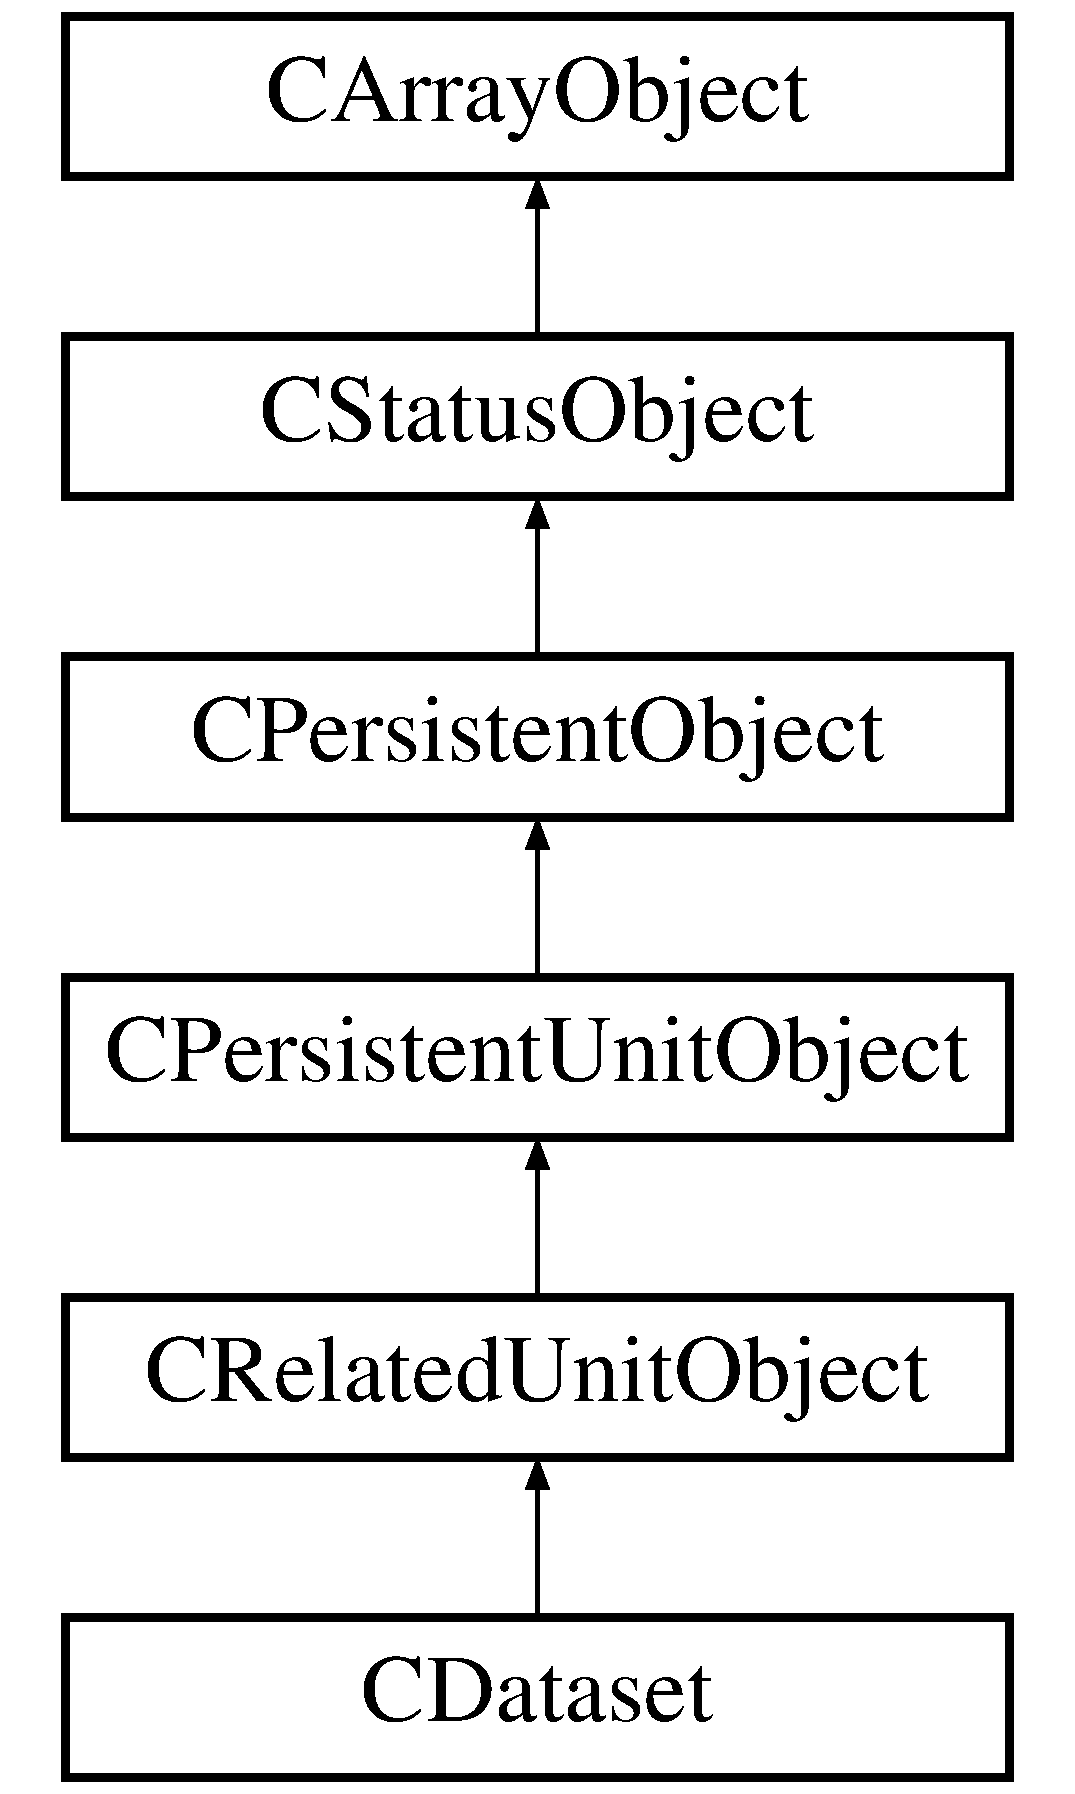
\includegraphics[height=5.000000cm]{class_c_dataset}
\end{center}
\end{figure}
\subsection*{Public Member Functions}
\begin{DoxyCompactItemize}
\item 
\hyperlink{class_c_dataset_ac98f85ed4391e12f46101e706720c718}{Code} (\$the\-Value=N\-U\-L\-L, \$get\-Old=F\-A\-L\-S\-E)
\end{DoxyCompactItemize}


\subsection{Member Function Documentation}
\hypertarget{class_c_dataset_ac98f85ed4391e12f46101e706720c718}{\index{C\-Dataset@{C\-Dataset}!Code@{Code}}
\index{Code@{Code}!CDataset@{C\-Dataset}}
\subsubsection[{Code}]{\setlength{\rightskip}{0pt plus 5cm}{\bf C\-Dataset\-::\-Code} (
\begin{DoxyParamCaption}
\item[{\$}]{the\-Value = {\ttfamily NULL}, }
\item[{\$}]{get\-Old = {\ttfamily FALSE}}
\end{DoxyParamCaption}
)}}\label{class_c_dataset_ac98f85ed4391e12f46101e706720c718}
Manage user code.

This method can be used to manage the user \hyperlink{}{code}, it uses the standard accessor \hyperlink{class_c_array_object_a931cb8b30569b811a18adc0161eb3603}{method} to manage the \hyperlink{}{offset}\-:


\begin{DoxyItemize}
\item {\bfseries \$the\-Value}\-: The value or operation\-: 
\begin{DoxyItemize}
\item {\itshape N\-U\-L\-L\/}\-: Return the current value. 
\item {\itshape F\-A\-L\-S\-E\/}\-: Delete the value. 
\item {\itshape other\/}\-: Set value. 
\end{DoxyItemize}
\item {\bfseries \$get\-Old}\-: Determines what the method will return\-: 
\begin{DoxyItemize}
\item {\itshape T\-R\-U\-E\/}\-: Return the value {\itshape before\/} it was eventually modified. 
\item {\itshape F\-A\-L\-S\-E\/}\-: Return the value {\itshape after\/} it was eventually modified. 
\end{DoxyItemize}
\end{DoxyItemize}


\begin{DoxyParams}[1]{Parameters}
N\-U\-L\-L | F\-A\-L\-S\-E | string & {\em \$the\-Value} & User code or operation. \\
\hline
boolean & {\em \$get\-Old} & T\-R\-U\-E get old value.\\
\hline
\end{DoxyParams}
public \begin{DoxyReturn}{Returns}
string 
\end{DoxyReturn}


The documentation for this class was generated from the following file\-:\begin{DoxyCompactItemize}
\item 
/\-Library/\-Web\-Server/\-Library/wrapper/classes/C\-Dataset.\-php\end{DoxyCompactItemize}

\hypertarget{class_c_data_wrapper}{\section{C\-Data\-Wrapper Class Reference}
\label{class_c_data_wrapper}\index{C\-Data\-Wrapper@{C\-Data\-Wrapper}}
}
Inheritance diagram for C\-Data\-Wrapper\-:\begin{figure}[H]
\begin{center}
\leavevmode
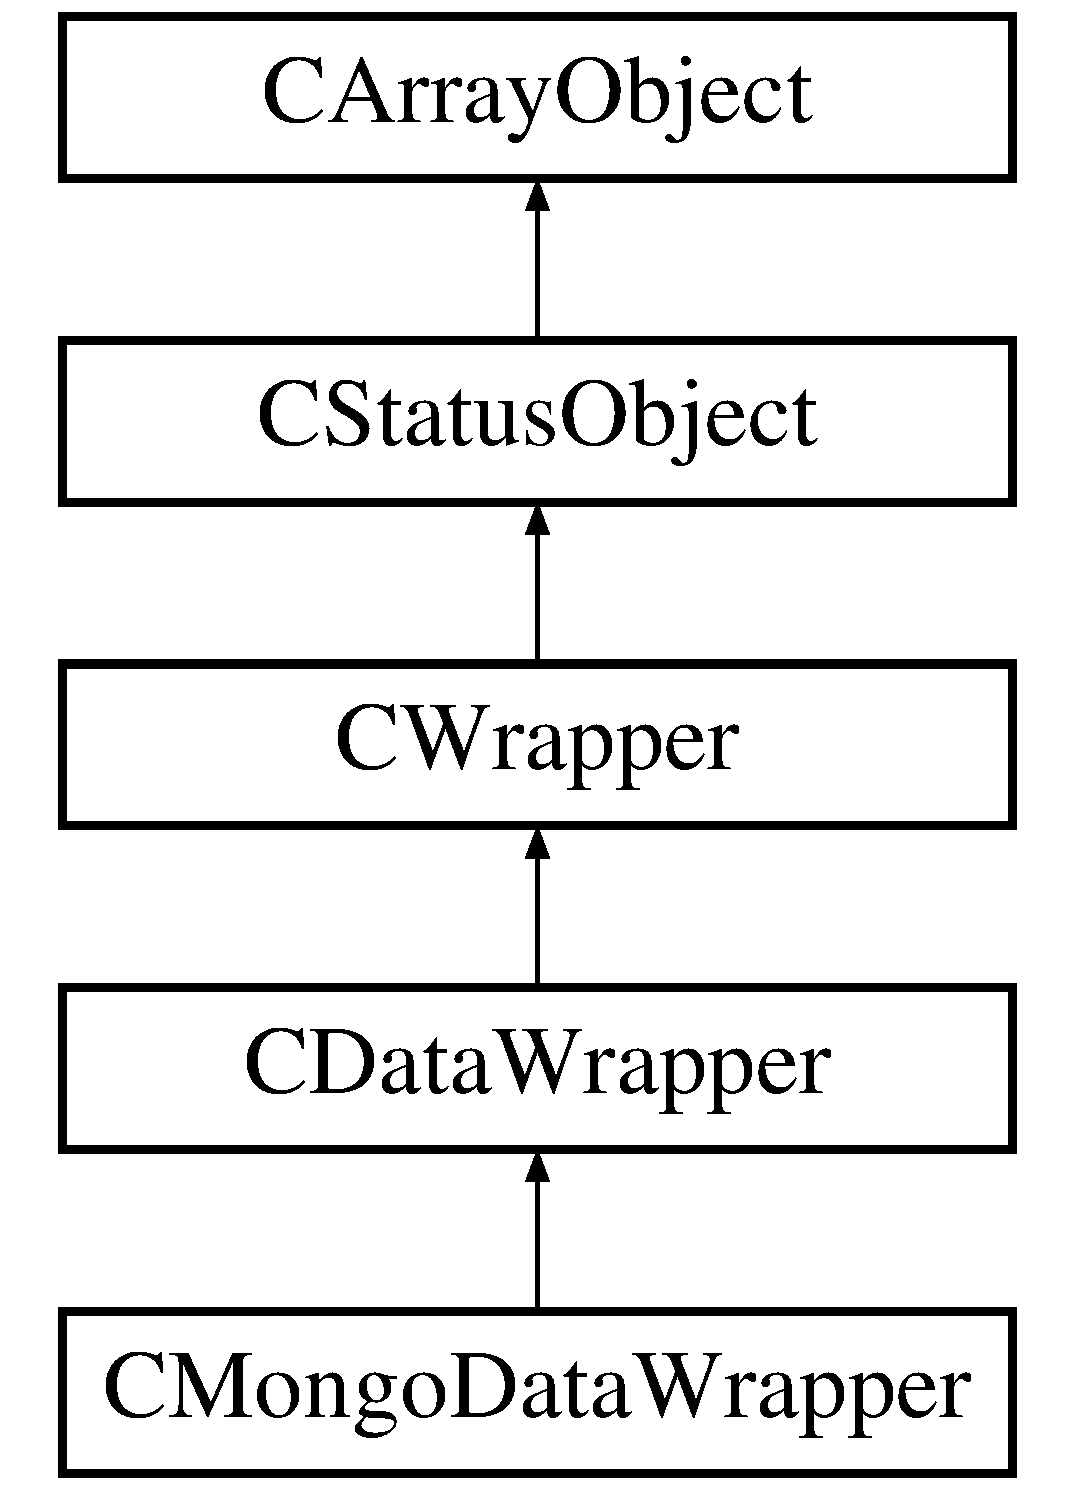
\includegraphics[height=5.000000cm]{class_c_data_wrapper}
\end{center}
\end{figure}
\subsection*{Protected Member Functions}
\begin{DoxyCompactItemize}
\item 
\hyperlink{class_c_data_wrapper_a85c97add738d08f2f2a9958ffbda6c03}{\-\_\-\-Init\-Options} ()
\item 
\hyperlink{class_c_data_wrapper_a8b42bd195d9ec6b38ef8e0df3f5dba7a}{\-\_\-\-Parse\-Request} ()
\item 
\hyperlink{class_c_data_wrapper_ab46c0e9797e8636ca1c9d535b377b90a}{\-\_\-\-Format\-Request} ()
\item 
\hyperlink{class_c_data_wrapper_aed059c9ffcb6e988633ba5b28a875b76}{\-\_\-\-Validate\-Request} ()
\item 
\hyperlink{class_c_data_wrapper_a3a0153df5d8c9e29e53d5060b78de785}{\-\_\-\-Parse\-Paging} ()
\item 
\hyperlink{class_c_data_wrapper_afdf0880393aff6f06b29a03245bed4a5}{\-\_\-\-Parse\-Database} ()
\item 
\hyperlink{class_c_data_wrapper_a7f0f78bd3a8528562275fb6cbb2f161d}{\-\_\-\-Parse\-Container} ()
\item 
\hyperlink{class_c_data_wrapper_a3b0852a34c7e36ae691fa6afdfe78856}{\-\_\-\-Parse\-Query} ()
\item 
\hyperlink{class_c_data_wrapper_aea29d199dc406381b85260ec2179aa16}{\-\_\-\-Parse\-Fields} ()
\item 
\hyperlink{class_c_data_wrapper_a73cd0698e6eb033bf5500be06d3c9814}{\-\_\-\-Parse\-Sort} ()
\item 
\hyperlink{class_c_data_wrapper_ab8f321158c05c2db991c35fa43b7b652}{\-\_\-\-Parse\-Object} ()
\item 
\hyperlink{class_c_data_wrapper_a7d02707497013c19b13cbbe5bd6be8b3}{\-\_\-\-Parse\-Options} ()
\item 
\hyperlink{class_c_data_wrapper_a0c3054fcf3716d638922cd581d5c706e}{\-\_\-\-Format\-Query} ()
\item 
\hyperlink{class_c_data_wrapper_a32f71d08b69799b48dc341bc2e9e998f}{\-\_\-\-Format\-Fields} ()
\item 
\hyperlink{class_c_data_wrapper_a040ed6e140436322b736744740cc8cbd}{\-\_\-\-Format\-Sort} ()
\item 
\hyperlink{class_c_data_wrapper_addefb7bd419de62bfebedc21abbdad7e}{\-\_\-\-Format\-Object} ()
\item 
\hyperlink{class_c_data_wrapper_a42bf6e7d0710dac687ca4c5d40983b5f}{\-\_\-\-Format\-Options} ()
\item 
\hyperlink{class_c_data_wrapper_ac25dbab0dc8d55b3b8f0a4027d4549c6}{\-\_\-\-Validate\-Operation} ()
\item 
\hyperlink{class_c_data_wrapper_a5bcbbc659ee704bca8e7c111ec5f1d0c}{\-\_\-\-Validate\-Fields} ()
\item 
\hyperlink{class_c_data_wrapper_a42d14abef174cd5eddee8e050faf3268}{\-\_\-\-Validate\-Sort} ()
\item 
\hyperlink{class_c_data_wrapper_afd3cc0f380334934e54d6fba1b954438}{\-\_\-\-Validate\-Options} ()
\item 
\hyperlink{class_c_data_wrapper_a30617297259d0ec38f793db4e1bb115d}{\-\_\-\-Decode\-Parameter} (\$the\-Parameter)
\end{DoxyCompactItemize}


\subsection{Member Function Documentation}
\hypertarget{class_c_data_wrapper_a30617297259d0ec38f793db4e1bb115d}{\index{C\-Data\-Wrapper@{C\-Data\-Wrapper}!\-\_\-\-Decode\-Parameter@{\-\_\-\-Decode\-Parameter}}
\index{\-\_\-\-Decode\-Parameter@{\-\_\-\-Decode\-Parameter}!CDataWrapper@{C\-Data\-Wrapper}}
\subsubsection[{\-\_\-\-Decode\-Parameter}]{\setlength{\rightskip}{0pt plus 5cm}{\bf C\-Data\-Wrapper\-::\-\_\-\-Decode\-Parameter} (
\begin{DoxyParamCaption}
\item[{\$}]{the\-Parameter}
\end{DoxyParamCaption}
)\hspace{0.3cm}{\ttfamily  \mbox{[}protected\mbox{]}}}}\label{class_c_data_wrapper_a30617297259d0ec38f793db4e1bb115d}
Decode parameter.

This method can be used to decode a parameter according to the provided format, \hyperlink{}{J\-S\-O\-N} or \hyperlink{}{P\-H\-P}.

The method will return the decoded parameter.


\begin{DoxyParams}[1]{Parameters}
string & {\em \$the\-Parameter} & Parameter offset.\\
\hline
\end{DoxyParams}
private \begin{DoxyReturn}{Returns}
array
\end{DoxyReturn}
\hyperlink{class_c_object_a06eb0f5acf83d67bda8f7946cade841e}{C\-Object\-::\-Json\-Decode()}

\begin{DoxySeeAlso}{See also}
k\-D\-A\-T\-A\-\_\-\-T\-Y\-P\-E\-\_\-\-J\-S\-O\-N k\-D\-A\-T\-A\-\_\-\-T\-Y\-P\-E\-\_\-\-P\-H\-P 
\end{DoxySeeAlso}
\hypertarget{class_c_data_wrapper_a32f71d08b69799b48dc341bc2e9e998f}{\index{C\-Data\-Wrapper@{C\-Data\-Wrapper}!\-\_\-\-Format\-Fields@{\-\_\-\-Format\-Fields}}
\index{\-\_\-\-Format\-Fields@{\-\_\-\-Format\-Fields}!CDataWrapper@{C\-Data\-Wrapper}}
\subsubsection[{\-\_\-\-Format\-Fields}]{\setlength{\rightskip}{0pt plus 5cm}{\bf C\-Data\-Wrapper\-::\-\_\-\-Format\-Fields} (
\begin{DoxyParamCaption}
{}
\end{DoxyParamCaption}
)\hspace{0.3cm}{\ttfamily  \mbox{[}protected\mbox{]}}}}\label{class_c_data_wrapper_a32f71d08b69799b48dc341bc2e9e998f}
Format fields.

This method will format the request fields.

private

\hyperlink{class_c_data_wrapper_a30617297259d0ec38f793db4e1bb115d}{\-\_\-\-Decode\-Parameter()}

\begin{DoxySeeAlso}{See also}
k\-A\-P\-I\-\_\-\-D\-A\-T\-A\-\_\-\-F\-I\-E\-L\-D 
\end{DoxySeeAlso}
\hypertarget{class_c_data_wrapper_addefb7bd419de62bfebedc21abbdad7e}{\index{C\-Data\-Wrapper@{C\-Data\-Wrapper}!\-\_\-\-Format\-Object@{\-\_\-\-Format\-Object}}
\index{\-\_\-\-Format\-Object@{\-\_\-\-Format\-Object}!CDataWrapper@{C\-Data\-Wrapper}}
\subsubsection[{\-\_\-\-Format\-Object}]{\setlength{\rightskip}{0pt plus 5cm}{\bf C\-Data\-Wrapper\-::\-\_\-\-Format\-Object} (
\begin{DoxyParamCaption}
{}
\end{DoxyParamCaption}
)\hspace{0.3cm}{\ttfamily  \mbox{[}protected\mbox{]}}}}\label{class_c_data_wrapper_addefb7bd419de62bfebedc21abbdad7e}
Format object.

This method will format the request object.

private

\hyperlink{class_c_data_wrapper_a30617297259d0ec38f793db4e1bb115d}{\-\_\-\-Decode\-Parameter()}

\begin{DoxySeeAlso}{See also}
k\-A\-P\-I\-\_\-\-D\-A\-T\-A\-\_\-\-O\-B\-J\-E\-C\-T 
\end{DoxySeeAlso}


Reimplemented in \hyperlink{class_c_mongo_data_wrapper_a2642638da121e471c7ea1fbb61f6f3ef}{C\-Mongo\-Data\-Wrapper}.

\hypertarget{class_c_data_wrapper_a42bf6e7d0710dac687ca4c5d40983b5f}{\index{C\-Data\-Wrapper@{C\-Data\-Wrapper}!\-\_\-\-Format\-Options@{\-\_\-\-Format\-Options}}
\index{\-\_\-\-Format\-Options@{\-\_\-\-Format\-Options}!CDataWrapper@{C\-Data\-Wrapper}}
\subsubsection[{\-\_\-\-Format\-Options}]{\setlength{\rightskip}{0pt plus 5cm}{\bf C\-Data\-Wrapper\-::\-\_\-\-Format\-Options} (
\begin{DoxyParamCaption}
{}
\end{DoxyParamCaption}
)\hspace{0.3cm}{\ttfamily  \mbox{[}protected\mbox{]}}}}\label{class_c_data_wrapper_a42bf6e7d0710dac687ca4c5d40983b5f}
Format options.

This method will format the request options.

private

\hyperlink{class_c_data_wrapper_a30617297259d0ec38f793db4e1bb115d}{\-\_\-\-Decode\-Parameter()}

\begin{DoxySeeAlso}{See also}
k\-A\-P\-I\-\_\-\-D\-A\-T\-A\-\_\-\-O\-P\-T\-I\-O\-N\-S 
\end{DoxySeeAlso}
\hypertarget{class_c_data_wrapper_a0c3054fcf3716d638922cd581d5c706e}{\index{C\-Data\-Wrapper@{C\-Data\-Wrapper}!\-\_\-\-Format\-Query@{\-\_\-\-Format\-Query}}
\index{\-\_\-\-Format\-Query@{\-\_\-\-Format\-Query}!CDataWrapper@{C\-Data\-Wrapper}}
\subsubsection[{\-\_\-\-Format\-Query}]{\setlength{\rightskip}{0pt plus 5cm}{\bf C\-Data\-Wrapper\-::\-\_\-\-Format\-Query} (
\begin{DoxyParamCaption}
{}
\end{DoxyParamCaption}
)\hspace{0.3cm}{\ttfamily  \mbox{[}protected\mbox{]}}}}\label{class_c_data_wrapper_a0c3054fcf3716d638922cd581d5c706e}
Format query.

This method will format the request query.

private

\hyperlink{class_c_data_wrapper_a30617297259d0ec38f793db4e1bb115d}{\-\_\-\-Decode\-Parameter()}

\begin{DoxySeeAlso}{See also}
k\-A\-P\-I\-\_\-\-D\-A\-T\-A\-\_\-\-Q\-U\-E\-R\-Y 
\end{DoxySeeAlso}


Reimplemented in \hyperlink{class_c_mongo_data_wrapper_a807db77c3c4f7708e86873a0447b83ff}{C\-Mongo\-Data\-Wrapper}.

\hypertarget{class_c_data_wrapper_ab46c0e9797e8636ca1c9d535b377b90a}{\index{C\-Data\-Wrapper@{C\-Data\-Wrapper}!\-\_\-\-Format\-Request@{\-\_\-\-Format\-Request}}
\index{\-\_\-\-Format\-Request@{\-\_\-\-Format\-Request}!CDataWrapper@{C\-Data\-Wrapper}}
\subsubsection[{\-\_\-\-Format\-Request}]{\setlength{\rightskip}{0pt plus 5cm}{\bf C\-Data\-Wrapper\-::\-\_\-\-Format\-Request} (
\begin{DoxyParamCaption}
{}
\end{DoxyParamCaption}
)\hspace{0.3cm}{\ttfamily  \mbox{[}protected\mbox{]}}}}\label{class_c_data_wrapper_ab46c0e9797e8636ca1c9d535b377b90a}
Format request.

This method should perform any needed formatting before the request will be handled.

In this class we handle the parameters to be decoded

private

\hyperlink{class_c_data_wrapper_ab46c0e9797e8636ca1c9d535b377b90a}{\-\_\-\-Format\-Request()}  \hyperlink{class_c_data_wrapper_a0c3054fcf3716d638922cd581d5c706e}{\-\_\-\-Format\-Query()}  \hyperlink{class_c_data_wrapper_a32f71d08b69799b48dc341bc2e9e998f}{\-\_\-\-Format\-Fields()}  \hyperlink{class_c_data_wrapper_a040ed6e140436322b736744740cc8cbd}{\-\_\-\-Format\-Sort()}  \hyperlink{class_c_data_wrapper_addefb7bd419de62bfebedc21abbdad7e}{\-\_\-\-Format\-Object()}  \hyperlink{class_c_data_wrapper_a42bf6e7d0710dac687ca4c5d40983b5f}{\-\_\-\-Format\-Options()} 

Reimplemented from \hyperlink{class_c_wrapper_a2a3d95961650654468789883ab1607e5}{C\-Wrapper}.



Reimplemented in \hyperlink{class_c_mongo_data_wrapper_abbc0d41394dda4a27eefa8481065749a}{C\-Mongo\-Data\-Wrapper}.

\hypertarget{class_c_data_wrapper_a040ed6e140436322b736744740cc8cbd}{\index{C\-Data\-Wrapper@{C\-Data\-Wrapper}!\-\_\-\-Format\-Sort@{\-\_\-\-Format\-Sort}}
\index{\-\_\-\-Format\-Sort@{\-\_\-\-Format\-Sort}!CDataWrapper@{C\-Data\-Wrapper}}
\subsubsection[{\-\_\-\-Format\-Sort}]{\setlength{\rightskip}{0pt plus 5cm}{\bf C\-Data\-Wrapper\-::\-\_\-\-Format\-Sort} (
\begin{DoxyParamCaption}
{}
\end{DoxyParamCaption}
)\hspace{0.3cm}{\ttfamily  \mbox{[}protected\mbox{]}}}}\label{class_c_data_wrapper_a040ed6e140436322b736744740cc8cbd}
Format sort.

This method will format the request sort.

private

\hyperlink{class_c_data_wrapper_a30617297259d0ec38f793db4e1bb115d}{\-\_\-\-Decode\-Parameter()}

\begin{DoxySeeAlso}{See also}
k\-A\-P\-I\-\_\-\-D\-A\-T\-A\-\_\-\-S\-O\-R\-T 
\end{DoxySeeAlso}
\hypertarget{class_c_data_wrapper_a85c97add738d08f2f2a9958ffbda6c03}{\index{C\-Data\-Wrapper@{C\-Data\-Wrapper}!\-\_\-\-Init\-Options@{\-\_\-\-Init\-Options}}
\index{\-\_\-\-Init\-Options@{\-\_\-\-Init\-Options}!CDataWrapper@{C\-Data\-Wrapper}}
\subsubsection[{\-\_\-\-Init\-Options}]{\setlength{\rightskip}{0pt plus 5cm}{\bf C\-Data\-Wrapper\-::\-\_\-\-Init\-Options} (
\begin{DoxyParamCaption}
{}
\end{DoxyParamCaption}
)\hspace{0.3cm}{\ttfamily  \mbox{[}protected\mbox{]}}}}\label{class_c_data_wrapper_a85c97add738d08f2f2a9958ffbda6c03}
Initialise options.

We overload this method to normalise the \hyperlink{}{paging} options.

private

\begin{DoxySeeAlso}{See also}
k\-A\-P\-I\-\_\-\-P\-A\-G\-E\-\_\-\-S\-T\-A\-R\-T k\-A\-P\-I\-\_\-\-P\-A\-G\-E\-\_\-\-L\-I\-M\-I\-T k\-A\-P\-I\-\_\-\-D\-A\-T\-A\-\_\-\-P\-A\-G\-I\-N\-G 
\end{DoxySeeAlso}


Reimplemented from \hyperlink{class_c_wrapper_aec2fa3594e36a380d66743b47c24490c}{C\-Wrapper}.

\hypertarget{class_c_data_wrapper_a7f0f78bd3a8528562275fb6cbb2f161d}{\index{C\-Data\-Wrapper@{C\-Data\-Wrapper}!\-\_\-\-Parse\-Container@{\-\_\-\-Parse\-Container}}
\index{\-\_\-\-Parse\-Container@{\-\_\-\-Parse\-Container}!CDataWrapper@{C\-Data\-Wrapper}}
\subsubsection[{\-\_\-\-Parse\-Container}]{\setlength{\rightskip}{0pt plus 5cm}{\bf C\-Data\-Wrapper\-::\-\_\-\-Parse\-Container} (
\begin{DoxyParamCaption}
{}
\end{DoxyParamCaption}
)\hspace{0.3cm}{\ttfamily  \mbox{[}protected\mbox{]}}}}\label{class_c_data_wrapper_a7f0f78bd3a8528562275fb6cbb2f161d}
Parse container.

This method will parse the request container.

private

\hyperlink{class_c_wrapper_aff9eb1799c8f30cb33967c7a50ce6395}{\-\_\-\-Offset\-Manage()}

\begin{DoxySeeAlso}{See also}
k\-A\-P\-I\-\_\-\-C\-O\-N\-T\-A\-I\-N\-E\-R k\-A\-P\-I\-\_\-\-D\-A\-T\-A\-\_\-\-R\-E\-Q\-U\-E\-S\-T 
\end{DoxySeeAlso}
\hypertarget{class_c_data_wrapper_afdf0880393aff6f06b29a03245bed4a5}{\index{C\-Data\-Wrapper@{C\-Data\-Wrapper}!\-\_\-\-Parse\-Database@{\-\_\-\-Parse\-Database}}
\index{\-\_\-\-Parse\-Database@{\-\_\-\-Parse\-Database}!CDataWrapper@{C\-Data\-Wrapper}}
\subsubsection[{\-\_\-\-Parse\-Database}]{\setlength{\rightskip}{0pt plus 5cm}{\bf C\-Data\-Wrapper\-::\-\_\-\-Parse\-Database} (
\begin{DoxyParamCaption}
{}
\end{DoxyParamCaption}
)\hspace{0.3cm}{\ttfamily  \mbox{[}protected\mbox{]}}}}\label{class_c_data_wrapper_afdf0880393aff6f06b29a03245bed4a5}
Parse database.

This method will parse the request database.

private

\hyperlink{class_c_wrapper_aff9eb1799c8f30cb33967c7a50ce6395}{\-\_\-\-Offset\-Manage()}

\begin{DoxySeeAlso}{See also}
k\-A\-P\-I\-\_\-\-D\-A\-T\-A\-B\-A\-S\-E k\-A\-P\-I\-\_\-\-D\-A\-T\-A\-\_\-\-R\-E\-Q\-U\-E\-S\-T 
\end{DoxySeeAlso}
\hypertarget{class_c_data_wrapper_aea29d199dc406381b85260ec2179aa16}{\index{C\-Data\-Wrapper@{C\-Data\-Wrapper}!\-\_\-\-Parse\-Fields@{\-\_\-\-Parse\-Fields}}
\index{\-\_\-\-Parse\-Fields@{\-\_\-\-Parse\-Fields}!CDataWrapper@{C\-Data\-Wrapper}}
\subsubsection[{\-\_\-\-Parse\-Fields}]{\setlength{\rightskip}{0pt plus 5cm}{\bf C\-Data\-Wrapper\-::\-\_\-\-Parse\-Fields} (
\begin{DoxyParamCaption}
{}
\end{DoxyParamCaption}
)\hspace{0.3cm}{\ttfamily  \mbox{[}protected\mbox{]}}}}\label{class_c_data_wrapper_aea29d199dc406381b85260ec2179aa16}
Parse fields.

This method will parse the request fields.

private

\hyperlink{class_c_wrapper_aff9eb1799c8f30cb33967c7a50ce6395}{\-\_\-\-Offset\-Manage()}

\begin{DoxySeeAlso}{See also}
k\-A\-P\-I\-\_\-\-D\-A\-T\-A\-\_\-\-F\-I\-E\-L\-D k\-A\-P\-I\-\_\-\-D\-A\-T\-A\-\_\-\-R\-E\-Q\-U\-E\-S\-T 
\end{DoxySeeAlso}
\hypertarget{class_c_data_wrapper_ab8f321158c05c2db991c35fa43b7b652}{\index{C\-Data\-Wrapper@{C\-Data\-Wrapper}!\-\_\-\-Parse\-Object@{\-\_\-\-Parse\-Object}}
\index{\-\_\-\-Parse\-Object@{\-\_\-\-Parse\-Object}!CDataWrapper@{C\-Data\-Wrapper}}
\subsubsection[{\-\_\-\-Parse\-Object}]{\setlength{\rightskip}{0pt plus 5cm}{\bf C\-Data\-Wrapper\-::\-\_\-\-Parse\-Object} (
\begin{DoxyParamCaption}
{}
\end{DoxyParamCaption}
)\hspace{0.3cm}{\ttfamily  \mbox{[}protected\mbox{]}}}}\label{class_c_data_wrapper_ab8f321158c05c2db991c35fa43b7b652}
Parse object.

This method will parse the request object.

private

\hyperlink{class_c_wrapper_aff9eb1799c8f30cb33967c7a50ce6395}{\-\_\-\-Offset\-Manage()}

\begin{DoxySeeAlso}{See also}
k\-A\-P\-I\-\_\-\-D\-A\-T\-A\-\_\-\-O\-B\-J\-E\-C\-T k\-A\-P\-I\-\_\-\-D\-A\-T\-A\-\_\-\-R\-E\-Q\-U\-E\-S\-T 
\end{DoxySeeAlso}
\hypertarget{class_c_data_wrapper_a7d02707497013c19b13cbbe5bd6be8b3}{\index{C\-Data\-Wrapper@{C\-Data\-Wrapper}!\-\_\-\-Parse\-Options@{\-\_\-\-Parse\-Options}}
\index{\-\_\-\-Parse\-Options@{\-\_\-\-Parse\-Options}!CDataWrapper@{C\-Data\-Wrapper}}
\subsubsection[{\-\_\-\-Parse\-Options}]{\setlength{\rightskip}{0pt plus 5cm}{\bf C\-Data\-Wrapper\-::\-\_\-\-Parse\-Options} (
\begin{DoxyParamCaption}
{}
\end{DoxyParamCaption}
)\hspace{0.3cm}{\ttfamily  \mbox{[}protected\mbox{]}}}}\label{class_c_data_wrapper_a7d02707497013c19b13cbbe5bd6be8b3}
Parse options.

This method will parse the request options.

private

\hyperlink{class_c_wrapper_aff9eb1799c8f30cb33967c7a50ce6395}{\-\_\-\-Offset\-Manage()}

\begin{DoxySeeAlso}{See also}
k\-A\-P\-I\-\_\-\-D\-A\-T\-A\-\_\-\-O\-P\-T\-I\-O\-N\-S k\-A\-P\-I\-\_\-\-D\-A\-T\-A\-\_\-\-R\-E\-Q\-U\-E\-S\-T 
\end{DoxySeeAlso}
\hypertarget{class_c_data_wrapper_a3a0153df5d8c9e29e53d5060b78de785}{\index{C\-Data\-Wrapper@{C\-Data\-Wrapper}!\-\_\-\-Parse\-Paging@{\-\_\-\-Parse\-Paging}}
\index{\-\_\-\-Parse\-Paging@{\-\_\-\-Parse\-Paging}!CDataWrapper@{C\-Data\-Wrapper}}
\subsubsection[{\-\_\-\-Parse\-Paging}]{\setlength{\rightskip}{0pt plus 5cm}{\bf C\-Data\-Wrapper\-::\-\_\-\-Parse\-Paging} (
\begin{DoxyParamCaption}
{}
\end{DoxyParamCaption}
)\hspace{0.3cm}{\ttfamily  \mbox{[}protected\mbox{]}}}}\label{class_c_data_wrapper_a3a0153df5d8c9e29e53d5060b78de785}
Parse paging.

This method will parse the request pager.

private

\hyperlink{class_c_wrapper_aff9eb1799c8f30cb33967c7a50ce6395}{\-\_\-\-Offset\-Manage()}

\begin{DoxySeeAlso}{See also}
k\-A\-P\-I\-\_\-\-P\-A\-G\-E\-\_\-\-S\-T\-A\-R\-T k\-A\-P\-I\-\_\-\-P\-A\-G\-E\-\_\-\-L\-I\-M\-I\-T k\-A\-P\-I\-\_\-\-D\-A\-T\-A\-\_\-\-P\-A\-G\-I\-N\-G k\-A\-P\-I\-\_\-\-D\-A\-T\-A\-\_\-\-R\-E\-Q\-U\-E\-S\-T 
\end{DoxySeeAlso}
\hypertarget{class_c_data_wrapper_a3b0852a34c7e36ae691fa6afdfe78856}{\index{C\-Data\-Wrapper@{C\-Data\-Wrapper}!\-\_\-\-Parse\-Query@{\-\_\-\-Parse\-Query}}
\index{\-\_\-\-Parse\-Query@{\-\_\-\-Parse\-Query}!CDataWrapper@{C\-Data\-Wrapper}}
\subsubsection[{\-\_\-\-Parse\-Query}]{\setlength{\rightskip}{0pt plus 5cm}{\bf C\-Data\-Wrapper\-::\-\_\-\-Parse\-Query} (
\begin{DoxyParamCaption}
{}
\end{DoxyParamCaption}
)\hspace{0.3cm}{\ttfamily  \mbox{[}protected\mbox{]}}}}\label{class_c_data_wrapper_a3b0852a34c7e36ae691fa6afdfe78856}
Parse query.

This method will parse the request query.

private

\hyperlink{class_c_wrapper_aff9eb1799c8f30cb33967c7a50ce6395}{\-\_\-\-Offset\-Manage()}

\begin{DoxySeeAlso}{See also}
k\-A\-P\-I\-\_\-\-D\-A\-T\-A\-\_\-\-Q\-U\-E\-R\-Y k\-A\-P\-I\-\_\-\-D\-A\-T\-A\-\_\-\-R\-E\-Q\-U\-E\-S\-T 
\end{DoxySeeAlso}
\hypertarget{class_c_data_wrapper_a8b42bd195d9ec6b38ef8e0df3f5dba7a}{\index{C\-Data\-Wrapper@{C\-Data\-Wrapper}!\-\_\-\-Parse\-Request@{\-\_\-\-Parse\-Request}}
\index{\-\_\-\-Parse\-Request@{\-\_\-\-Parse\-Request}!CDataWrapper@{C\-Data\-Wrapper}}
\subsubsection[{\-\_\-\-Parse\-Request}]{\setlength{\rightskip}{0pt plus 5cm}{\bf C\-Data\-Wrapper\-::\-\_\-\-Parse\-Request} (
\begin{DoxyParamCaption}
{}
\end{DoxyParamCaption}
)\hspace{0.3cm}{\ttfamily  \mbox{[}protected\mbox{]}}}}\label{class_c_data_wrapper_a8b42bd195d9ec6b38ef8e0df3f5dba7a}
Parse request.

This method should be used to parse the request, check the request elements and make any necessary adjustments before the request is \hyperlink{class_c_data_wrapper_aed059c9ffcb6e988633ba5b28a875b76}{validated}.

This is also where the relevant request elements will be logged to the relative response sections.

The method is called by the \hyperlink{class_c_wrapper_a683094b01e0682fd34926562d7a052e0}{constructor} and should be overloaded to handle derived classes custom elements.

In this class we handle the paging request.

private

\hyperlink{class_c_data_wrapper_a8b42bd195d9ec6b38ef8e0df3f5dba7a}{\-\_\-\-Parse\-Request()}  \hyperlink{class_c_data_wrapper_a3a0153df5d8c9e29e53d5060b78de785}{\-\_\-\-Parse\-Paging()}  \hyperlink{class_c_data_wrapper_afdf0880393aff6f06b29a03245bed4a5}{\-\_\-\-Parse\-Database()}  \hyperlink{class_c_data_wrapper_a7f0f78bd3a8528562275fb6cbb2f161d}{\-\_\-\-Parse\-Container()}  \hyperlink{class_c_data_wrapper_a3b0852a34c7e36ae691fa6afdfe78856}{\-\_\-\-Parse\-Query()}  \hyperlink{class_c_data_wrapper_aea29d199dc406381b85260ec2179aa16}{\-\_\-\-Parse\-Fields()}  \hyperlink{class_c_data_wrapper_a73cd0698e6eb033bf5500be06d3c9814}{\-\_\-\-Parse\-Sort()}  \hyperlink{class_c_data_wrapper_ab8f321158c05c2db991c35fa43b7b652}{\-\_\-\-Parse\-Object()}  \hyperlink{class_c_data_wrapper_a7d02707497013c19b13cbbe5bd6be8b3}{\-\_\-\-Parse\-Options()} 

Reimplemented from \hyperlink{class_c_wrapper_a6675c744053f1b05547ad28fc50a79e6}{C\-Wrapper}.

\hypertarget{class_c_data_wrapper_a73cd0698e6eb033bf5500be06d3c9814}{\index{C\-Data\-Wrapper@{C\-Data\-Wrapper}!\-\_\-\-Parse\-Sort@{\-\_\-\-Parse\-Sort}}
\index{\-\_\-\-Parse\-Sort@{\-\_\-\-Parse\-Sort}!CDataWrapper@{C\-Data\-Wrapper}}
\subsubsection[{\-\_\-\-Parse\-Sort}]{\setlength{\rightskip}{0pt plus 5cm}{\bf C\-Data\-Wrapper\-::\-\_\-\-Parse\-Sort} (
\begin{DoxyParamCaption}
{}
\end{DoxyParamCaption}
)\hspace{0.3cm}{\ttfamily  \mbox{[}protected\mbox{]}}}}\label{class_c_data_wrapper_a73cd0698e6eb033bf5500be06d3c9814}
Parse sort.

This method will parse the request sort.

private

\hyperlink{class_c_wrapper_aff9eb1799c8f30cb33967c7a50ce6395}{\-\_\-\-Offset\-Manage()}

\begin{DoxySeeAlso}{See also}
k\-A\-P\-I\-\_\-\-D\-A\-T\-A\-\_\-\-S\-O\-R\-T k\-A\-P\-I\-\_\-\-D\-A\-T\-A\-\_\-\-R\-E\-Q\-U\-E\-S\-T 
\end{DoxySeeAlso}
\hypertarget{class_c_data_wrapper_a5bcbbc659ee704bca8e7c111ec5f1d0c}{\index{C\-Data\-Wrapper@{C\-Data\-Wrapper}!\-\_\-\-Validate\-Fields@{\-\_\-\-Validate\-Fields}}
\index{\-\_\-\-Validate\-Fields@{\-\_\-\-Validate\-Fields}!CDataWrapper@{C\-Data\-Wrapper}}
\subsubsection[{\-\_\-\-Validate\-Fields}]{\setlength{\rightskip}{0pt plus 5cm}{\bf C\-Data\-Wrapper\-::\-\_\-\-Validate\-Fields} (
\begin{DoxyParamCaption}
{}
\end{DoxyParamCaption}
)\hspace{0.3cm}{\ttfamily  \mbox{[}protected\mbox{]}}}}\label{class_c_data_wrapper_a5bcbbc659ee704bca8e7c111ec5f1d0c}
Validate field selection reference.

This method can be used to check whether the provided \hyperlink{}{field} parameter is valid.

In this class we ensure that the fields list is an array.

private

\begin{DoxySeeAlso}{See also}
k\-A\-P\-I\-\_\-\-D\-A\-T\-A\-\_\-\-F\-I\-E\-L\-D 
\end{DoxySeeAlso}
\hypertarget{class_c_data_wrapper_ac25dbab0dc8d55b3b8f0a4027d4549c6}{\index{C\-Data\-Wrapper@{C\-Data\-Wrapper}!\-\_\-\-Validate\-Operation@{\-\_\-\-Validate\-Operation}}
\index{\-\_\-\-Validate\-Operation@{\-\_\-\-Validate\-Operation}!CDataWrapper@{C\-Data\-Wrapper}}
\subsubsection[{\-\_\-\-Validate\-Operation}]{\setlength{\rightskip}{0pt plus 5cm}{\bf C\-Data\-Wrapper\-::\-\_\-\-Validate\-Operation} (
\begin{DoxyParamCaption}
{}
\end{DoxyParamCaption}
)\hspace{0.3cm}{\ttfamily  \mbox{[}protected\mbox{]}}}}\label{class_c_data_wrapper_ac25dbab0dc8d55b3b8f0a4027d4549c6}
Validate request operation.

This method can be used to check whether the provided \hyperlink{}{operation} parameter is valid.

private

\begin{DoxySeeAlso}{See also}
k\-A\-P\-I\-\_\-\-O\-P\-E\-R\-A\-T\-I\-O\-N k\-A\-P\-I\-\_\-\-O\-P\-\_\-\-S\-E\-T k\-A\-P\-I\-\_\-\-O\-P\-\_\-\-I\-N\-S\-E\-R\-T 

k\-A\-P\-I\-\_\-\-D\-A\-T\-A\-B\-A\-S\-E k\-A\-P\-I\-\_\-\-C\-O\-N\-T\-A\-I\-N\-E\-R k\-A\-P\-I\-\_\-\-D\-A\-T\-A\-\_\-\-O\-B\-J\-E\-C\-T k\-A\-P\-I\-\_\-\-D\-A\-T\-A\-\_\-\-Q\-U\-E\-R\-Y 
\end{DoxySeeAlso}


Reimplemented from \hyperlink{class_c_wrapper_aab3f7b2ca4cd9e692c35510d753918a4}{C\-Wrapper}.



Reimplemented in \hyperlink{class_c_mongo_data_wrapper_a406b81115b5f3957e6d40ee49ae85a13}{C\-Mongo\-Data\-Wrapper}.

\hypertarget{class_c_data_wrapper_afd3cc0f380334934e54d6fba1b954438}{\index{C\-Data\-Wrapper@{C\-Data\-Wrapper}!\-\_\-\-Validate\-Options@{\-\_\-\-Validate\-Options}}
\index{\-\_\-\-Validate\-Options@{\-\_\-\-Validate\-Options}!CDataWrapper@{C\-Data\-Wrapper}}
\subsubsection[{\-\_\-\-Validate\-Options}]{\setlength{\rightskip}{0pt plus 5cm}{\bf C\-Data\-Wrapper\-::\-\_\-\-Validate\-Options} (
\begin{DoxyParamCaption}
{}
\end{DoxyParamCaption}
)\hspace{0.3cm}{\ttfamily  \mbox{[}protected\mbox{]}}}}\label{class_c_data_wrapper_afd3cc0f380334934e54d6fba1b954438}
Validate sort selection reference.

This method can be used to check whether the provided \hyperlink{}{sort} parameter is valid.

In this class we ensure that the sort list is an array.

private

\begin{DoxySeeAlso}{See also}
k\-A\-P\-I\-\_\-\-D\-A\-T\-A\-\_\-\-O\-P\-T\-I\-O\-N\-S 
\end{DoxySeeAlso}
\hypertarget{class_c_data_wrapper_aed059c9ffcb6e988633ba5b28a875b76}{\index{C\-Data\-Wrapper@{C\-Data\-Wrapper}!\-\_\-\-Validate\-Request@{\-\_\-\-Validate\-Request}}
\index{\-\_\-\-Validate\-Request@{\-\_\-\-Validate\-Request}!CDataWrapper@{C\-Data\-Wrapper}}
\subsubsection[{\-\_\-\-Validate\-Request}]{\setlength{\rightskip}{0pt plus 5cm}{\bf C\-Data\-Wrapper\-::\-\_\-\-Validate\-Request} (
\begin{DoxyParamCaption}
{}
\end{DoxyParamCaption}
)\hspace{0.3cm}{\ttfamily  \mbox{[}protected\mbox{]}}}}\label{class_c_data_wrapper_aed059c9ffcb6e988633ba5b28a875b76}
Validate request.

This method should check that the request is valid and that all required parameters have been sent.

In this class we check the \hyperlink{}{format} and \hyperlink{}{operation} codes (their presence is checked by the \hyperlink{class_c_wrapper_a683094b01e0682fd34926562d7a052e0}{constructor}.

private

\hyperlink{class_c_data_wrapper_aed059c9ffcb6e988633ba5b28a875b76}{\-\_\-\-Validate\-Request()}  \hyperlink{class_c_data_wrapper_a5bcbbc659ee704bca8e7c111ec5f1d0c}{\-\_\-\-Validate\-Fields()}  \hyperlink{class_c_data_wrapper_a42d14abef174cd5eddee8e050faf3268}{\-\_\-\-Validate\-Sort()}  \hyperlink{class_c_data_wrapper_afd3cc0f380334934e54d6fba1b954438}{\-\_\-\-Validate\-Options()} 

Reimplemented from \hyperlink{class_c_wrapper_a24b22cfd0022c1cba1741fb294fba5ba}{C\-Wrapper}.



Reimplemented in \hyperlink{class_c_mongo_data_wrapper_a3d06376cb588e5c26751bff3f0083ef5}{C\-Mongo\-Data\-Wrapper}.

\hypertarget{class_c_data_wrapper_a42d14abef174cd5eddee8e050faf3268}{\index{C\-Data\-Wrapper@{C\-Data\-Wrapper}!\-\_\-\-Validate\-Sort@{\-\_\-\-Validate\-Sort}}
\index{\-\_\-\-Validate\-Sort@{\-\_\-\-Validate\-Sort}!CDataWrapper@{C\-Data\-Wrapper}}
\subsubsection[{\-\_\-\-Validate\-Sort}]{\setlength{\rightskip}{0pt plus 5cm}{\bf C\-Data\-Wrapper\-::\-\_\-\-Validate\-Sort} (
\begin{DoxyParamCaption}
{}
\end{DoxyParamCaption}
)\hspace{0.3cm}{\ttfamily  \mbox{[}protected\mbox{]}}}}\label{class_c_data_wrapper_a42d14abef174cd5eddee8e050faf3268}
Validate sort selection reference.

This method can be used to check whether the provided \hyperlink{}{sort} parameter is valid.

In this class we ensure that the sort list is an array.

private

\begin{DoxySeeAlso}{See also}
k\-A\-P\-I\-\_\-\-D\-A\-T\-A\-\_\-\-S\-O\-R\-T 
\end{DoxySeeAlso}


The documentation for this class was generated from the following file\-:\begin{DoxyCompactItemize}
\item 
/\-Library/\-Web\-Server/\-Library/wrapper/classes/C\-Data\-Wrapper.\-php\end{DoxyCompactItemize}

\hypertarget{class_c_entity}{\section{C\-Entity Class Reference}
\label{class_c_entity}\index{C\-Entity@{C\-Entity}}
}
Inheritance diagram for C\-Entity\-:\begin{figure}[H]
\begin{center}
\leavevmode
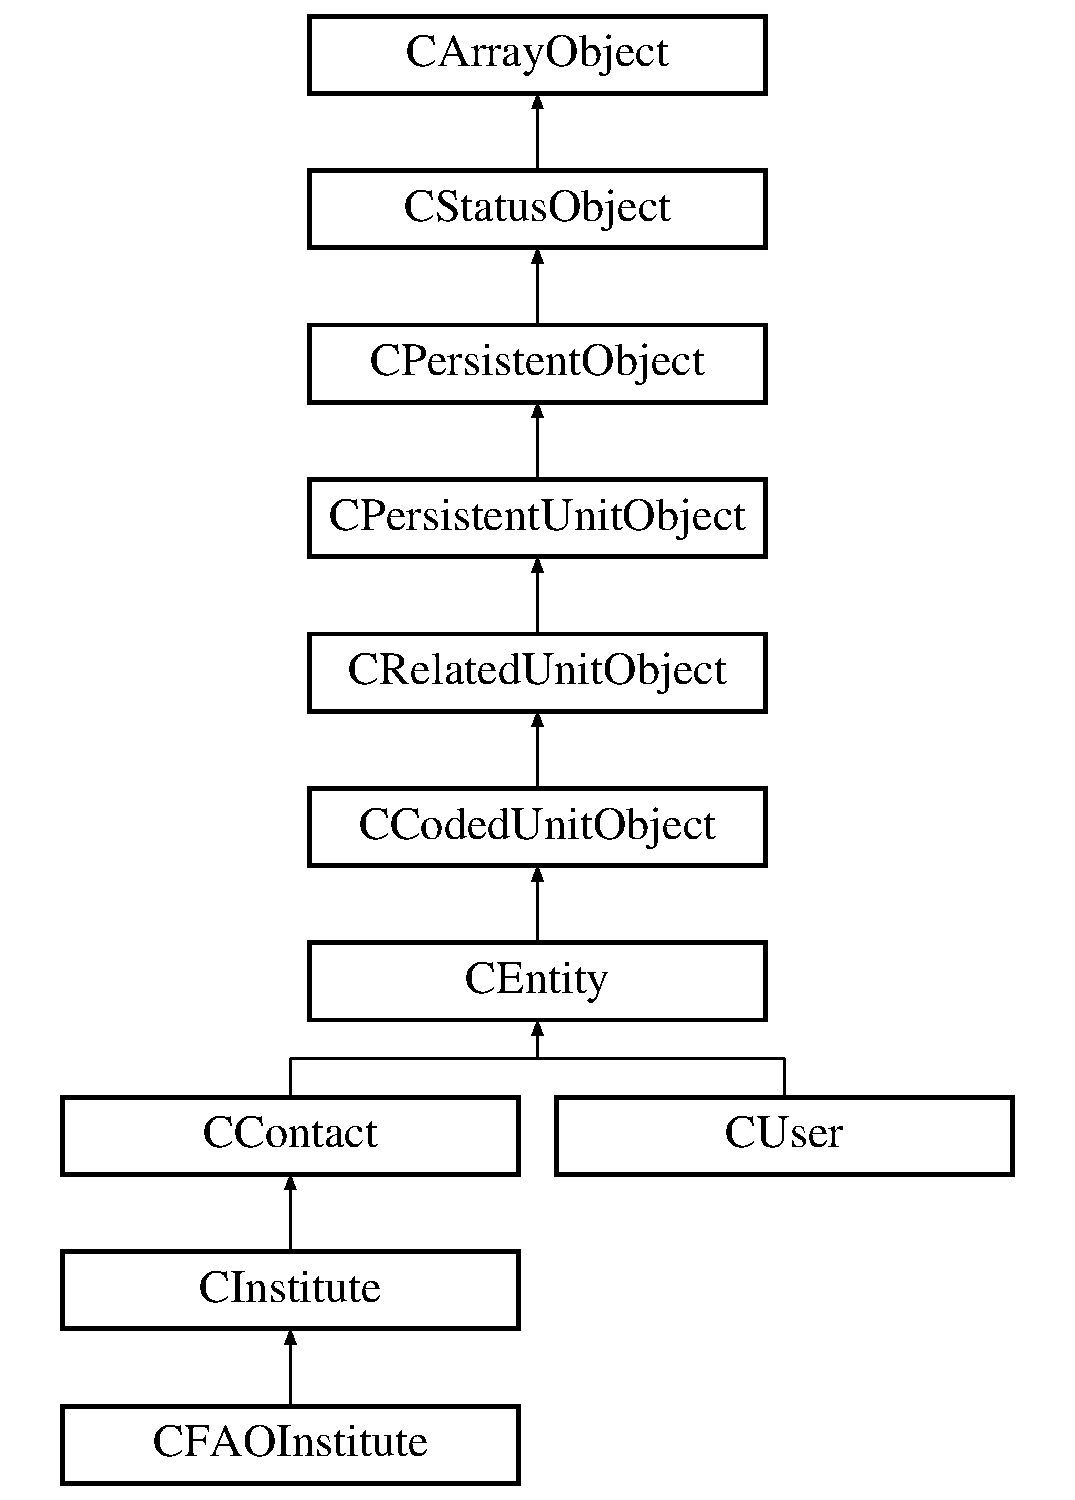
\includegraphics[height=6.000000cm]{class_c_entity}
\end{center}
\end{figure}
\subsection*{Public Member Functions}
\begin{DoxyCompactItemize}
\item 
\hyperlink{class_c_entity_ac087e5b3d14357f452ab531db5f6a7e9}{\-\_\-\-\_\-construct} (\$the\-Container=N\-U\-L\-L, \$the\-Identifier=N\-U\-L\-L)
\item 
\hyperlink{class_c_entity_a78127acb8de5ae1e7238566396dd1c17}{Type} (\$the\-Value=N\-U\-L\-L, \$the\-Operation=N\-U\-L\-L, \$get\-Old=F\-A\-L\-S\-E)
\item 
\hyperlink{class_c_entity_a2b3cf77715881c3d8b3a6d4d80042e7c}{Code} (\$the\-Value=N\-U\-L\-L, \$get\-Old=F\-A\-L\-S\-E)
\item 
\hyperlink{class_c_entity_ace5878c009baf09d85c8ca115c48dbb0}{Name} (\$the\-Value=N\-U\-L\-L, \$get\-Old=F\-A\-L\-S\-E)
\item 
\hyperlink{class_c_entity_a44b389a90107f4c8aadcc4eb08e1ad9b}{Mail} (\$the\-Type=N\-U\-L\-L, \$the\-Value=N\-U\-L\-L, \$get\-Old=F\-A\-L\-S\-E)
\item 
\hyperlink{class_c_entity_acf65b6fb2f4195f6c649b4ca506c7899}{Email} (\$the\-Value=N\-U\-L\-L, \$get\-Old=F\-A\-L\-S\-E)
\item 
\hyperlink{class_c_entity_ac69e40a0ee4489abfcc7241d98b07532}{Phone} (\$the\-Value=N\-U\-L\-L, \$get\-Old=F\-A\-L\-S\-E)
\item 
\hyperlink{class_c_entity_ac8fc97b7adfc8ce547db5f93a9b913a8}{Parent} (\$the\-Value, \$the\-Operation=N\-U\-L\-L, \$get\-Old=F\-A\-L\-S\-E)
\item 
\hyperlink{class_c_entity_a193cf3d19057021bb6e779644730eac8}{offset\-Set} (\$the\-Offset, \$the\-Value)
\item 
\hyperlink{class_c_entity_a887a87fc716e36a0d4c1477dbaf5bb67}{offset\-Unset} (\$the\-Offset)
\end{DoxyCompactItemize}
\subsection*{Static Public Member Functions}
\begin{DoxyCompactItemize}
\item 
static \hyperlink{class_c_entity_a260a4c309aff31a42d0e23b372f9b209}{Default\-Container} ()
\end{DoxyCompactItemize}
\subsection*{Protected Member Functions}
\begin{DoxyCompactItemize}
\item 
\hyperlink{class_c_entity_a991f328223b1b00b37e9028b16f7a7c8}{\-\_\-\-Prepare\-Store} (\&\$the\-Container, \&\$the\-Identifier)
\item 
\hyperlink{class_c_entity_ac518d3885e2c6f30051b8c5ec59e50a3}{\-\_\-id} ()
\end{DoxyCompactItemize}


\subsection{Constructor \& Destructor Documentation}
\hypertarget{class_c_entity_ac087e5b3d14357f452ab531db5f6a7e9}{\index{C\-Entity@{C\-Entity}!\-\_\-\-\_\-construct@{\-\_\-\-\_\-construct}}
\index{\-\_\-\-\_\-construct@{\-\_\-\-\_\-construct}!CEntity@{C\-Entity}}
\subsubsection[{\-\_\-\-\_\-construct}]{\setlength{\rightskip}{0pt plus 5cm}{\bf C\-Entity\-::\-\_\-\-\_\-construct} (
\begin{DoxyParamCaption}
\item[{\$}]{the\-Container = {\ttfamily NULL}, }
\item[{\$}]{the\-Identifier = {\ttfamily NULL}}
\end{DoxyParamCaption}
)}}\label{class_c_entity_ac087e5b3d14357f452ab531db5f6a7e9}
Instantiate class.

We \hyperlink{class_c_persistent_object_a10d0ce97598da33eaf305eb43e418255}{overload} the constructor to initialise the \hyperlink{class_c_status_object_a8429102e4f52f7558649b64f4e673a69}{inited} \hyperlink{}{flag} if the \hyperlink{class_c_entity_a2b3cf77715881c3d8b3a6d4d80042e7c}{code} and \hyperlink{class_c_entity_ace5878c009baf09d85c8ca115c48dbb0}{name} elements are set.


\begin{DoxyParams}[1]{Parameters}
mixed & {\em \$the\-Container} & Persistent container. \\
\hline
mixed & {\em \$the\-Identifier} & Object identifier.\\
\hline
\end{DoxyParams}
public 

Reimplemented from \hyperlink{class_c_persistent_object_a10d0ce97598da33eaf305eb43e418255}{C\-Persistent\-Object}.



Reimplemented in \hyperlink{class_c_user_a728ac6fd50a9f9e18dfe2fa547d5c798}{C\-User}.



\subsection{Member Function Documentation}
\hypertarget{class_c_entity_ac518d3885e2c6f30051b8c5ec59e50a3}{\index{C\-Entity@{C\-Entity}!\-\_\-id@{\-\_\-id}}
\index{\-\_\-id@{\-\_\-id}!CEntity@{C\-Entity}}
\subsubsection[{\-\_\-id}]{\setlength{\rightskip}{0pt plus 5cm}{\bf C\-Entity\-::\-\_\-id} (
\begin{DoxyParamCaption}
{}
\end{DoxyParamCaption}
)\hspace{0.3cm}{\ttfamily  \mbox{[}protected\mbox{]}}}}\label{class_c_entity_ac518d3885e2c6f30051b8c5ec59e50a3}
Return the object's unique identifier.

We overload this method to return the object's \hyperlink{}{identifier}, if it is set, or the object's \hyperlink{class_c_entity_a2b3cf77715881c3d8b3a6d4d80042e7c}{code}.

If none of the above are set, we call the parent method.

protected \begin{DoxyReturn}{Returns}
string 
\end{DoxyReturn}


Reimplemented from \hyperlink{class_c_persistent_unit_object_ad1ca0920cf0df3c24351402f9afbf34b}{C\-Persistent\-Unit\-Object}.

\hypertarget{class_c_entity_a991f328223b1b00b37e9028b16f7a7c8}{\index{C\-Entity@{C\-Entity}!\-\_\-\-Prepare\-Store@{\-\_\-\-Prepare\-Store}}
\index{\-\_\-\-Prepare\-Store@{\-\_\-\-Prepare\-Store}!CEntity@{C\-Entity}}
\subsubsection[{\-\_\-\-Prepare\-Store}]{\setlength{\rightskip}{0pt plus 5cm}{\bf C\-Entity\-::\-\_\-\-Prepare\-Store} (
\begin{DoxyParamCaption}
\item[{\&\$}]{the\-Container, }
\item[{\&\$}]{the\-Identifier}
\end{DoxyParamCaption}
)\hspace{0.3cm}{\ttfamily  \mbox{[}protected\mbox{]}}}}\label{class_c_entity_a991f328223b1b00b37e9028b16f7a7c8}
Normalise before a store.

We overload this method to check if the object in \hyperlink{class_c_status_object_a8429102e4f52f7558649b64f4e673a69}{initialised}, if this is not the case we raise an exception.


\begin{DoxyParams}[1]{Parameters}
reference & {\em \&\$the\-Container} & Object container. \\
\hline
reference & {\em \&\$the\-Identifier} & Object identifier.\\
\hline
\end{DoxyParams}
protected


\begin{DoxyExceptions}{Exceptions}
{\em \hyperlink{class_c_exception}{C\-Exception}} & \\
\hline
\end{DoxyExceptions}
\begin{DoxySeeAlso}{See also}
k\-E\-R\-R\-O\-R\-\_\-\-O\-P\-T\-I\-O\-N\-\_\-\-M\-I\-S\-S\-I\-N\-G 
\end{DoxySeeAlso}


Reimplemented from \hyperlink{class_c_persistent_unit_object_a42b46ccb307aa8038e5ed78819a23aa6}{C\-Persistent\-Unit\-Object}.



Reimplemented in \hyperlink{class_c_user_a031f5d13fe837cf445006ee21023bf3e}{C\-User}.

\hypertarget{class_c_entity_a2b3cf77715881c3d8b3a6d4d80042e7c}{\index{C\-Entity@{C\-Entity}!Code@{Code}}
\index{Code@{Code}!CEntity@{C\-Entity}}
\subsubsection[{Code}]{\setlength{\rightskip}{0pt plus 5cm}{\bf C\-Entity\-::\-Code} (
\begin{DoxyParamCaption}
\item[{\$}]{the\-Value = {\ttfamily NULL}, }
\item[{\$}]{get\-Old = {\ttfamily FALSE}}
\end{DoxyParamCaption}
)}}\label{class_c_entity_a2b3cf77715881c3d8b3a6d4d80042e7c}
Manage entity code.

This method can be used to manage the entity \hyperlink{}{code}, it uses the standard accessor \hyperlink{class_c_array_object_a931cb8b30569b811a18adc0161eb3603}{method} to manage the \hyperlink{}{offset}\-:

For a more in-\/depth reference of this method, please consult the \hyperlink{class_c_array_object_a931cb8b30569b811a18adc0161eb3603}{\-\_\-\-Manage\-Offset} method, in which the first parameter will be the constant \hyperlink{}{k\-T\-A\-G\-\_\-\-C\-O\-D\-E}.


\begin{DoxyParams}[1]{Parameters}
mixed & {\em \$the\-Value} & Value. \\
\hline
boolean & {\em \$get\-Old} & T\-R\-U\-E get old value.\\
\hline
\end{DoxyParams}
public \begin{DoxyReturn}{Returns}
string 
\end{DoxyReturn}
\hypertarget{class_c_entity_a260a4c309aff31a42d0e23b372f9b209}{\index{C\-Entity@{C\-Entity}!Default\-Container@{Default\-Container}}
\index{Default\-Container@{Default\-Container}!CEntity@{C\-Entity}}
\subsubsection[{Default\-Container}]{\setlength{\rightskip}{0pt plus 5cm}static {\bf C\-Entity\-::\-Default\-Container} (
\begin{DoxyParamCaption}
{}
\end{DoxyParamCaption}
)\hspace{0.3cm}{\ttfamily  \mbox{[}static\mbox{]}}}}\label{class_c_entity_a260a4c309aff31a42d0e23b372f9b209}
Return the default container.

This method can be used to retrieve the default container name.

\begin{DoxyReturn}{Returns}
string 
\end{DoxyReturn}
\hypertarget{class_c_entity_acf65b6fb2f4195f6c649b4ca506c7899}{\index{C\-Entity@{C\-Entity}!Email@{Email}}
\index{Email@{Email}!CEntity@{C\-Entity}}
\subsubsection[{Email}]{\setlength{\rightskip}{0pt plus 5cm}{\bf C\-Entity\-::\-Email} (
\begin{DoxyParamCaption}
\item[{\$}]{the\-Value = {\ttfamily NULL}, }
\item[{\$}]{get\-Old = {\ttfamily FALSE}}
\end{DoxyParamCaption}
)}}\label{class_c_entity_acf65b6fb2f4195f6c649b4ca506c7899}
Manage entity e-\/mail.

This method can be used to manage the entity \hyperlink{}{e-\/mail}, it uses the standard accessor \hyperlink{class_c_array_object_a931cb8b30569b811a18adc0161eb3603}{method} to manage the \hyperlink{}{offset}\-:

For a more in-\/depth reference of this method, please consult the \hyperlink{class_c_array_object_a931cb8b30569b811a18adc0161eb3603}{\-\_\-\-Manage\-Offset} method, in which the first parameter will be the constant \hyperlink{}{k\-O\-F\-F\-S\-E\-T\-\_\-\-E\-M\-A\-I\-L}.


\begin{DoxyParams}[1]{Parameters}
mixed & {\em \$the\-Value} & Value. \\
\hline
boolean & {\em \$get\-Old} & T\-R\-U\-E get old value.\\
\hline
\end{DoxyParams}
public \begin{DoxyReturn}{Returns}
string 
\end{DoxyReturn}
\hypertarget{class_c_entity_a44b389a90107f4c8aadcc4eb08e1ad9b}{\index{C\-Entity@{C\-Entity}!Mail@{Mail}}
\index{Mail@{Mail}!CEntity@{C\-Entity}}
\subsubsection[{Mail}]{\setlength{\rightskip}{0pt plus 5cm}{\bf C\-Entity\-::\-Mail} (
\begin{DoxyParamCaption}
\item[{\$}]{the\-Type = {\ttfamily NULL}, }
\item[{\$}]{the\-Value = {\ttfamily NULL}, }
\item[{\$}]{get\-Old = {\ttfamily FALSE}}
\end{DoxyParamCaption}
)}}\label{class_c_entity_a44b389a90107f4c8aadcc4eb08e1ad9b}
Manage entity mailing addresses.

This method can be used to manage the entity mailing \hyperlink{}{addresses}, it uses the standard accessor \hyperlink{class_c_array_object_af714f81bb75f725c6868fb286c59b160}{method} to manage the list of addresses.

This list is an array of structures where the \hyperlink{}{k\-T\-A\-G\-\_\-\-T\-Y\-P\-E} element indicates the type of the address, for instance {\itshape home\/} or office, and the \hyperlink{}{k\-T\-A\-G\-\_\-\-D\-A\-T\-A} element represents the actual address, be it a string or itself a structure holding the address elements. If the \hyperlink{}{k\-T\-A\-G\-\_\-\-T\-Y\-P\-E} element is missing, we assume it to be the default address.

For a more in-\/depth reference of this method, please consult the \hyperlink{class_c_array_object_a056b7a3218ffb9a2eb992c029124a669}{\-\_\-\-Manage\-Typed\-Array\-Offset} method, in which the first parameter will be the constant \hyperlink{}{k\-O\-F\-F\-S\-E\-T\-\_\-\-M\-A\-I\-L}.

Note that this method will $<$i$<$N\-O\-T work on an object that was \hyperlink{class_c_mongo_data_wrapper_a0d37f7b47e1a1ac48846f6d10d08d846}{serialised}.


\begin{DoxyParams}[1]{Parameters}
mixed & {\em \$the\-Type} & Item type. \\
\hline
mixed & {\em \$the\-Value} & Item value. \\
\hline
boolean & {\em \$get\-Old} & T\-R\-U\-E get old value.\\
\hline
\end{DoxyParams}
public \begin{DoxyReturn}{Returns}
string 
\end{DoxyReturn}
\hypertarget{class_c_entity_ace5878c009baf09d85c8ca115c48dbb0}{\index{C\-Entity@{C\-Entity}!Name@{Name}}
\index{Name@{Name}!CEntity@{C\-Entity}}
\subsubsection[{Name}]{\setlength{\rightskip}{0pt plus 5cm}{\bf C\-Entity\-::\-Name} (
\begin{DoxyParamCaption}
\item[{\$}]{the\-Value = {\ttfamily NULL}, }
\item[{\$}]{get\-Old = {\ttfamily FALSE}}
\end{DoxyParamCaption}
)}}\label{class_c_entity_ace5878c009baf09d85c8ca115c48dbb0}
Manage entity name.

This method can be used to manage the entity \hyperlink{}{name}, it uses the standard accessor \hyperlink{class_c_array_object_a931cb8b30569b811a18adc0161eb3603}{method} to manage the \hyperlink{}{offset}\-:

For a more in-\/depth reference of this method, please consult the \hyperlink{class_c_array_object_a931cb8b30569b811a18adc0161eb3603}{\-\_\-\-Manage\-Offset} method, in which the first parameter will be the constant \hyperlink{}{k\-T\-A\-G\-\_\-\-N\-A\-M\-E}.


\begin{DoxyParams}[1]{Parameters}
mixed & {\em \$the\-Value} & Value. \\
\hline
boolean & {\em \$get\-Old} & T\-R\-U\-E get old value.\\
\hline
\end{DoxyParams}
public \begin{DoxyReturn}{Returns}
string 
\end{DoxyReturn}
\hypertarget{class_c_entity_a193cf3d19057021bb6e779644730eac8}{\index{C\-Entity@{C\-Entity}!offset\-Set@{offset\-Set}}
\index{offset\-Set@{offset\-Set}!CEntity@{C\-Entity}}
\subsubsection[{offset\-Set}]{\setlength{\rightskip}{0pt plus 5cm}{\bf C\-Entity\-::offset\-Set} (
\begin{DoxyParamCaption}
\item[{\$}]{the\-Offset, }
\item[{\$}]{the\-Value}
\end{DoxyParamCaption}
)}}\label{class_c_entity_a193cf3d19057021bb6e779644730eac8}
Set a value for a given offset.

We overload this method to manage the \hyperlink{}{Inited() inited} \hyperlink{}{status}\-: this is set if \hyperlink{}{code} and \hyperlink{}{name} properties are set.


\begin{DoxyParams}[1]{Parameters}
string & {\em \$the\-Offset} & Offset. \\
\hline
string | N\-U\-L\-L & {\em \$the\-Value} & Value to set at offset.\\
\hline
\end{DoxyParams}
public 

Reimplemented from \hyperlink{class_c_status_object_a140ef140d4fa1c4a6180e843bd5ec969}{C\-Status\-Object}.



Reimplemented in \hyperlink{class_c_user_aace3446b9cacfe28cc1937c608fcc999}{C\-User}.

\hypertarget{class_c_entity_a887a87fc716e36a0d4c1477dbaf5bb67}{\index{C\-Entity@{C\-Entity}!offset\-Unset@{offset\-Unset}}
\index{offset\-Unset@{offset\-Unset}!CEntity@{C\-Entity}}
\subsubsection[{offset\-Unset}]{\setlength{\rightskip}{0pt plus 5cm}{\bf C\-Entity\-::offset\-Unset} (
\begin{DoxyParamCaption}
\item[{\$}]{the\-Offset}
\end{DoxyParamCaption}
)}}\label{class_c_entity_a887a87fc716e36a0d4c1477dbaf5bb67}
Reset a value for a given offset.

We overload this method to manage the \hyperlink{}{Inited() inited} \hyperlink{}{status}\-: this is set if \hyperlink{}{code} and \hyperlink{}{name} properties are set.


\begin{DoxyParams}[1]{Parameters}
string & {\em \$the\-Offset} & Offset.\\
\hline
\end{DoxyParams}
public 

Reimplemented from \hyperlink{class_c_status_object_ae733db1bbfffcbe894ea405765ab4150}{C\-Status\-Object}.



Reimplemented in \hyperlink{class_c_user_aed8557e18a89d868cedf5a48328b33b2}{C\-User}.

\hypertarget{class_c_entity_ac8fc97b7adfc8ce547db5f93a9b913a8}{\index{C\-Entity@{C\-Entity}!Parent@{Parent}}
\index{Parent@{Parent}!CEntity@{C\-Entity}}
\subsubsection[{Parent}]{\setlength{\rightskip}{0pt plus 5cm}{\bf C\-Entity\-::\-Parent} (
\begin{DoxyParamCaption}
\item[{\$}]{the\-Value, }
\item[{\$}]{the\-Operation = {\ttfamily NULL}, }
\item[{\$}]{get\-Old = {\ttfamily FALSE}}
\end{DoxyParamCaption}
)}}\label{class_c_entity_ac8fc97b7adfc8ce547db5f93a9b913a8}
Manage entity parents.

This method can be used to manage the entity \hyperlink{}{parents}, you can add/replace, retrieve and delete parent elements depending on the value of the parameters.

The property is represented by an array of instances derived from this class, or strings representing entity \hyperlink{}{identifiers}. In the first case, prior to \hyperlink{class_c_persistent_object_ad076a9a2baf73bba0784deb135a3b7b7}{saving} the current object, array elements in the form of \hyperlink{class_c_entity}{C\-Entity} instances will also be \hyperlink{class_c_persistent_object_ad076a9a2baf73bba0784deb135a3b7b7}{saved} and replaced by their \hyperlink{}{identifiers}.

This method accepts the following parameters\-:


\begin{DoxyItemize}
\item {\bfseries \$the\-Index}\-: This parameter represents the element index. 
\item {\bfseries \$the\-Operation}\-: The operation to perform\-: 
\begin{DoxyItemize}
\item {\itshape N\-U\-L\-L\/}\-: Retrieve the element, the methoid will return the matching element or {\itshape N\-U\-L\-L\/} if not found. 
\item {\itshape F\-A\-L\-S\-E\/}\-: Delete the element, depending on the value of the next parameter, the method will either return the deleted element or {\itshape N\-U\-L\-L\/}. 
\item {\itshape other\/}\-: Any other value means that we want to add/replace the element, in this case the method will return the added element's index. 
\end{DoxyItemize}
\item {\bfseries \$the\-Data}\-: This parameter represents the element data. 
\end{DoxyItemize}

Note that this method will $<$i$<$N\-O\-T work on an object that was \hyperlink{class_c_mongo_data_wrapper_a0d37f7b47e1a1ac48846f6d10d08d846}{serialised}.


\begin{DoxyParams}[1]{Parameters}
mixed & {\em \$the\-Value} & Index or value. \\
\hline
mixed & {\em \$the\-Operation} & Operation. \\
\hline
boolean & {\em \$get\-Old} & T\-R\-U\-E get old value.\\
\hline
\end{DoxyParams}
public \begin{DoxyReturn}{Returns}
string 
\end{DoxyReturn}
\hypertarget{class_c_entity_ac69e40a0ee4489abfcc7241d98b07532}{\index{C\-Entity@{C\-Entity}!Phone@{Phone}}
\index{Phone@{Phone}!CEntity@{C\-Entity}}
\subsubsection[{Phone}]{\setlength{\rightskip}{0pt plus 5cm}{\bf C\-Entity\-::\-Phone} (
\begin{DoxyParamCaption}
\item[{\$}]{the\-Value = {\ttfamily NULL}, }
\item[{\$}]{get\-Old = {\ttfamily FALSE}}
\end{DoxyParamCaption}
)}}\label{class_c_entity_ac69e40a0ee4489abfcc7241d98b07532}
Manage entity phone.

This method can be used to manage the entity \hyperlink{}{telephone} number, it uses the standard accessor \hyperlink{class_c_array_object_a931cb8b30569b811a18adc0161eb3603}{method} to manage the \hyperlink{}{offset}\-:

For a more in-\/depth reference of this method, please consult the \hyperlink{class_c_array_object_a931cb8b30569b811a18adc0161eb3603}{\-\_\-\-Manage\-Offset} method, in which the first parameter will be the constant \hyperlink{}{k\-O\-F\-F\-S\-E\-T\-\_\-\-P\-H\-O\-N\-E}.


\begin{DoxyParams}[1]{Parameters}
mixed & {\em \$the\-Value} & Value. \\
\hline
boolean & {\em \$get\-Old} & T\-R\-U\-E get old value.\\
\hline
\end{DoxyParams}
public \begin{DoxyReturn}{Returns}
string 
\end{DoxyReturn}
\hypertarget{class_c_entity_a78127acb8de5ae1e7238566396dd1c17}{\index{C\-Entity@{C\-Entity}!Type@{Type}}
\index{Type@{Type}!CEntity@{C\-Entity}}
\subsubsection[{Type}]{\setlength{\rightskip}{0pt plus 5cm}{\bf C\-Entity\-::\-Type} (
\begin{DoxyParamCaption}
\item[{\$}]{the\-Value = {\ttfamily NULL}, }
\item[{\$}]{the\-Operation = {\ttfamily NULL}, }
\item[{\$}]{get\-Old = {\ttfamily FALSE}}
\end{DoxyParamCaption}
)}}\label{class_c_entity_a78127acb8de5ae1e7238566396dd1c17}
Manage entity types.

This method can be used to manage the entity \hyperlink{}{types}, it uses the standard accessor \hyperlink{class_c_array_object_a056b7a3218ffb9a2eb992c029124a669}{method} to manage the list of parent entities.

In general, elements of this list should be a token that indicates a specific function of the entity, this could be, for instance', {\itshape user\/} to indicate an entity that is also a user of the system.

For a more in-\/depth reference of this method, please consult the \hyperlink{class_c_array_object_a056b7a3218ffb9a2eb992c029124a669}{\-\_\-\-Manage\-Array\-Offset} method, in which the first parameter will be the constant \hyperlink{}{k\-T\-A\-G\-\_\-\-T\-Y\-P\-E}.

Note that this method will $<$i$<$N\-O\-T work on an object that was \hyperlink{class_c_mongo_data_wrapper_a0d37f7b47e1a1ac48846f6d10d08d846}{serialised}.


\begin{DoxyParams}[1]{Parameters}
mixed & {\em \$the\-Value} & Value or index. \\
\hline
mixed & {\em \$the\-Operation} & Operation. \\
\hline
boolean & {\em \$get\-Old} & T\-R\-U\-E get old value.\\
\hline
\end{DoxyParams}
public \begin{DoxyReturn}{Returns}
string 
\end{DoxyReturn}


The documentation for this class was generated from the following file\-:\begin{DoxyCompactItemize}
\item 
/\-Library/\-Web\-Server/\-Library/wrapper/classes/C\-Entity.\-php\end{DoxyCompactItemize}

\hypertarget{class_c_exception}{\section{C\-Exception Class Reference}
\label{class_c_exception}\index{C\-Exception@{C\-Exception}}
}
\subsection*{Public Member Functions}
\begin{DoxyCompactItemize}
\item 
\hyperlink{class_c_exception_aea9f2ae76b6058652dfb672ce1a78507}{\-\_\-\-\_\-construct} (\$the\-Message=N\-U\-L\-L, \$the\-Code=N\-U\-L\-L, \$the\-Severity=N\-U\-L\-L, \$the\-References=N\-U\-L\-L, \$the\-Previous=N\-U\-L\-L)
\item 
\hyperlink{class_c_exception_a06b1b207799f8a8ca27bc12d1be82b07}{\-\_\-\-\_\-to\-String} ()
\item 
\hyperlink{class_c_exception_a2bef90da8a35e80dda8072d4f748ec20}{Severity} (\$the\-Value=N\-U\-L\-L)
\item 
\hyperlink{class_c_exception_abcbd46a262790fcbe3493e30a6418821}{Reference} (\$the\-Index=N\-U\-L\-L, \$the\-Value=N\-U\-L\-L)
\end{DoxyCompactItemize}
\subsection*{Static Public Member Functions}
\begin{DoxyCompactItemize}
\item 
static \hyperlink{class_c_exception_a99be238dee92094374995eebe54df6a8}{As\-H\-T\-M\-L} (Exception \$the\-Exception)
\item 
static \hyperlink{class_c_exception_ad5f92d9c5d11443ce4b69aec6a8484d5}{\-\_\-\-Trace} (Exception \$the\-Exception)
\item 
static \hyperlink{class_c_exception_a643b0ad0d3d4faba071968c953d639af}{\-\_\-\-Trace2\-H\-T\-M\-L} (D\-O\-M\-Node \$the\-Table, \$the\-Element)
\item 
static \hyperlink{class_c_exception_a84a97fbcc2907c16a29a01adf841ee94}{\-\_\-\-Exception2\-H\-T\-M\-L} (\$the\-Table, \$the\-Element, \$the\-Source=N\-U\-L\-L)
\end{DoxyCompactItemize}
\subsection*{Protected Member Functions}
\begin{DoxyCompactItemize}
\item 
\hyperlink{class_c_exception_a2fb444dcf37f658f1f5dc696ed35dd7d}{\-\_\-\-Trace\-Argument\-String} (\$the\-Value)
\end{DoxyCompactItemize}
\subsection*{Protected Attributes}
\begin{DoxyCompactItemize}
\item 
\hypertarget{class_c_exception_aa544b648ee9ef87c6bea3571737f10f6}{{\bfseries \$m\-Severity} = N\-U\-L\-L}\label{class_c_exception_aa544b648ee9ef87c6bea3571737f10f6}

\item 
\hypertarget{class_c_exception_a483fdc73c7a4726532dff474c97a4eb7}{{\bfseries \$m\-References} = Array()}\label{class_c_exception_a483fdc73c7a4726532dff474c97a4eb7}

\end{DoxyCompactItemize}


\subsection{Constructor \& Destructor Documentation}
\hypertarget{class_c_exception_aea9f2ae76b6058652dfb672ce1a78507}{\index{C\-Exception@{C\-Exception}!\-\_\-\-\_\-construct@{\-\_\-\-\_\-construct}}
\index{\-\_\-\-\_\-construct@{\-\_\-\-\_\-construct}!CException@{C\-Exception}}
\subsubsection[{\-\_\-\-\_\-construct}]{\setlength{\rightskip}{0pt plus 5cm}C\-Exception\-::\-\_\-\-\_\-construct (
\begin{DoxyParamCaption}
\item[{}]{\$the\-Message = {\ttfamily NULL}, }
\item[{}]{\$the\-Code = {\ttfamily NULL}, }
\item[{}]{\$the\-Severity = {\ttfamily NULL}, }
\item[{}]{\$the\-References = {\ttfamily NULL}, }
\item[{}]{\$the\-Previous = {\ttfamily NULL}}
\end{DoxyParamCaption}
)}}\label{class_c_exception_aea9f2ae76b6058652dfb672ce1a78507}
Instantiate class.

The first two parameters follow the inherited interface, the constructor adds support for the extended class members\-:


\begin{DoxyItemize}
\item {\bfseries \$the\-Message}\-: This parameter represents the inherited {\itshape message}. 
\item {\bfseries \$the\-Code}\-: This parameter represents the inherited {\itshape code}. 
\item {\bfseries \$the\-Severity}\-: This parameter holds \hyperlink{class_c_exception_a2bef90da8a35e80dda8072d4f748ec20}{the} exception type, level or severity\-: 
\begin{DoxyItemize}
\item {\itshape \hyperlink{}{k\-M\-E\-S\-S\-A\-G\-E\-\_\-\-T\-Y\-P\-E\-\_\-\-I\-D\-L\-E}}\-: This indicates an idle state. 
\item {\itshape \hyperlink{}{k\-M\-E\-S\-S\-A\-G\-E\-\_\-\-T\-Y\-P\-E\-\_\-\-N\-O\-T\-I\-C\-E}}\-: This indicates an informative note or message. 
\item {\itshape \hyperlink{}{k\-M\-E\-S\-S\-A\-G\-E\-\_\-\-T\-Y\-P\-E\-\_\-\-W\-A\-R\-N\-I\-N\-G}}\-: This indicates a warning. 
\item {\itshape \hyperlink{}{k\-M\-E\-S\-S\-A\-G\-E\-\_\-\-T\-Y\-P\-E\-\_\-\-E\-R\-R\-O\-R}}\-: This indicates an error. 
\item {\itshape \hyperlink{}{k\-M\-E\-S\-S\-A\-G\-E\-\_\-\-T\-Y\-P\-E\-\_\-\-F\-A\-T\-A\-L}}\-: This indicates a fatal error, in general this should halt program execution. 
\item {\itshape \hyperlink{}{k\-M\-E\-S\-S\-A\-G\-E\-\_\-\-T\-Y\-P\-E\-\_\-\-B\-U\-G}}\-: This indicates a bug, such exceptions should be logged and forwarded to developers. 
\end{DoxyItemize}
\item {\bfseries \$the\-References}\-: This parameter holds the exception's references \hyperlink{}{list}, it is an array indexed by reference label or term holding the reference value as value. 
\item {\bfseries \$the\-Previous}\-: This parameter represents the previous exception when forwarding. 
\end{DoxyItemize}


\begin{DoxyParams}[1]{Parameters}
string & {\em \$the\-Message} & Exception message. \\
\hline
integer & {\em \$the\-Code} & Exception code. \\
\hline
string & {\em \$the\-Severity} & Exception severity. \\
\hline
array & {\em \$the\-References} & Exception references. \\
\hline
Exception & {\em \$the\-Previous} & Previous exception.\\
\hline
\end{DoxyParams}
public

Code\-User()  User\-Messages()  User\-Namespace()  \hyperlink{class_c_exception_a2bef90da8a35e80dda8072d4f748ec20}{Severity()}  \hyperlink{class_c_exception_abcbd46a262790fcbe3493e30a6418821}{Reference()} 

\subsection{Member Function Documentation}
\hypertarget{class_c_exception_a06b1b207799f8a8ca27bc12d1be82b07}{\index{C\-Exception@{C\-Exception}!\-\_\-\-\_\-to\-String@{\-\_\-\-\_\-to\-String}}
\index{\-\_\-\-\_\-to\-String@{\-\_\-\-\_\-to\-String}!CException@{C\-Exception}}
\subsubsection[{\-\_\-\-\_\-to\-String}]{\setlength{\rightskip}{0pt plus 5cm}C\-Exception\-::\-\_\-\-\_\-to\-String (
\begin{DoxyParamCaption}
{}
\end{DoxyParamCaption}
)}}\label{class_c_exception_a06b1b207799f8a8ca27bc12d1be82b07}
Return the object name.

In this class we return the stack trace.

public \begin{DoxyReturn}{Returns}
string The stack trace. 
\end{DoxyReturn}
\hypertarget{class_c_exception_a84a97fbcc2907c16a29a01adf841ee94}{\index{C\-Exception@{C\-Exception}!\-\_\-\-Exception2\-H\-T\-M\-L@{\-\_\-\-Exception2\-H\-T\-M\-L}}
\index{\-\_\-\-Exception2\-H\-T\-M\-L@{\-\_\-\-Exception2\-H\-T\-M\-L}!CException@{C\-Exception}}
\subsubsection[{\-\_\-\-Exception2\-H\-T\-M\-L}]{\setlength{\rightskip}{0pt plus 5cm}static C\-Exception\-::\-\_\-\-Exception2\-H\-T\-M\-L (
\begin{DoxyParamCaption}
\item[{}]{\$the\-Table, }
\item[{}]{\$the\-Element, }
\item[{}]{\$the\-Source = {\ttfamily NULL}}
\end{DoxyParamCaption}
)\hspace{0.3cm}{\ttfamily [static]}}}\label{class_c_exception_a84a97fbcc2907c16a29a01adf841ee94}
Return the exception as H\-T\-M\-L.

This method can be used to return the provided exception as H\-T\-M\-L code, it is assumed that the element will be placed in an H\-T\-M\-L table, so the method will return a series of table rows.

The method accepts the following parameters\-:


\begin{DoxyItemize}
\item {\bfseries \$the\-Table}\-: The H\-T\-M\-L table in which we want to place the trace. 
\item {\bfseries \$the\-Element}\-: The exception, it must be an Exception, if any other type is passed, the method will return {\itshape N\-U\-L\-L}. 
\item {\bfseries \$the\-Source}\-: This parameter is used to provide a link to the source file\-: 
\begin{DoxyItemize}
\item {\itshape N\-U\-L\-L}\-: No source file management. 
\item {\itshape T\-R\-U\-E}\-: The default source file viewer will be used. 
\item {\itshape string}\-: The method will execute the provided string as a shell command line. 
\end{DoxyItemize}
\end{DoxyItemize}


\begin{DoxyParams}[1]{Parameters}
array & {\em \$the\-Element} & Trace element. \\
\hline
N\-U\-L\-L | T\-R\-U\-E | string & {\em \$the\-Source} & Source file control. \\
\hline
\end{DoxyParams}
\hypertarget{class_c_exception_ad5f92d9c5d11443ce4b69aec6a8484d5}{\index{C\-Exception@{C\-Exception}!\-\_\-\-Trace@{\-\_\-\-Trace}}
\index{\-\_\-\-Trace@{\-\_\-\-Trace}!CException@{C\-Exception}}
\subsubsection[{\-\_\-\-Trace}]{\setlength{\rightskip}{0pt plus 5cm}static C\-Exception\-::\-\_\-\-Trace (
\begin{DoxyParamCaption}
\item[{Exception}]{\$the\-Exception}
\end{DoxyParamCaption}
)\hspace{0.3cm}{\ttfamily [static]}}}\label{class_c_exception_ad5f92d9c5d11443ce4b69aec6a8484d5}
Return the exception trace.

This method can be used to return the exception trace in the order in which it was called. The main utility of this method is to manage forwarded exceptions.

The method will return an array indexed by file path and line number hash in which the value is either an exception or a trace array. If you run in P\-H\-P version $<$ 3.\-0.\-x the first element will be an exception and the others will be traces, if you run a higher version of P\-H\-P you can forward exceptions, so the elements will be mixed.


\begin{DoxyParams}[1]{Parameters}
Exception & {\em \$the\-Exception} & Exception to trace.\\
\hline
\end{DoxyParams}
\begin{DoxyReturn}{Returns}
array 
\end{DoxyReturn}
\hypertarget{class_c_exception_a643b0ad0d3d4faba071968c953d639af}{\index{C\-Exception@{C\-Exception}!\-\_\-\-Trace2\-H\-T\-M\-L@{\-\_\-\-Trace2\-H\-T\-M\-L}}
\index{\-\_\-\-Trace2\-H\-T\-M\-L@{\-\_\-\-Trace2\-H\-T\-M\-L}!CException@{C\-Exception}}
\subsubsection[{\-\_\-\-Trace2\-H\-T\-M\-L}]{\setlength{\rightskip}{0pt plus 5cm}static C\-Exception\-::\-\_\-\-Trace2\-H\-T\-M\-L (
\begin{DoxyParamCaption}
\item[{D\-O\-M\-Node}]{\$the\-Table, }
\item[{}]{\$the\-Element}
\end{DoxyParamCaption}
)\hspace{0.3cm}{\ttfamily [static]}}}\label{class_c_exception_a643b0ad0d3d4faba071968c953d639af}
Return the exception trace element as H\-T\-M\-L.

This method can be used to return the trace element as H\-T\-M\-L code.

The method accepts the following parameters\-:


\begin{DoxyItemize}
\item {\bfseries \$the\-Table}\-: The H\-T\-M\-L table in which we want to place the trace. 
\item {\bfseries \$the\-Element}\-: The trace element, it must be an array, if any other type is passed, the method will return {\itshape N\-U\-L\-L}. 
\end{DoxyItemize}


\begin{DoxyParams}[1]{Parameters}
D\-O\-M\-Node & {\em \$the\-Table} & H\-T\-M\-L table. \\
\hline
array & {\em \$the\-Element} & Trace element. \\
\hline
\end{DoxyParams}
\hypertarget{class_c_exception_a2fb444dcf37f658f1f5dc696ed35dd7d}{\index{C\-Exception@{C\-Exception}!\-\_\-\-Trace\-Argument\-String@{\-\_\-\-Trace\-Argument\-String}}
\index{\-\_\-\-Trace\-Argument\-String@{\-\_\-\-Trace\-Argument\-String}!CException@{C\-Exception}}
\subsubsection[{\-\_\-\-Trace\-Argument\-String}]{\setlength{\rightskip}{0pt plus 5cm}C\-Exception\-::\-\_\-\-Trace\-Argument\-String (
\begin{DoxyParamCaption}
\item[{}]{\$the\-Value}
\end{DoxyParamCaption}
)\hspace{0.3cm}{\ttfamily [protected]}}}\label{class_c_exception_a2fb444dcf37f658f1f5dc696ed35dd7d}
Return the trace argument string.

This method can be used to return the string representation of a trace argument.


\begin{DoxyParams}[1]{Parameters}
mixed & {\em \$the\-Value} & Trace argument.\\
\hline
\end{DoxyParams}
protected \begin{DoxyReturn}{Returns}
string 
\end{DoxyReturn}
\hypertarget{class_c_exception_a99be238dee92094374995eebe54df6a8}{\index{C\-Exception@{C\-Exception}!As\-H\-T\-M\-L@{As\-H\-T\-M\-L}}
\index{As\-H\-T\-M\-L@{As\-H\-T\-M\-L}!CException@{C\-Exception}}
\subsubsection[{As\-H\-T\-M\-L}]{\setlength{\rightskip}{0pt plus 5cm}static C\-Exception\-::\-As\-H\-T\-M\-L (
\begin{DoxyParamCaption}
\item[{Exception}]{\$the\-Exception}
\end{DoxyParamCaption}
)\hspace{0.3cm}{\ttfamily [static]}}}\label{class_c_exception_a99be238dee92094374995eebe54df6a8}
Display an exception.

This method can be used to display exceptions in a web browser page.


\begin{DoxyParams}[1]{Parameters}
Exception | \hyperlink{class_c_exception}{C\-Exception} & {\em \$the\-Exception} & Exception object.\\
\hline
\end{DoxyParams}
\begin{DoxyReturn}{Returns}
string
\end{DoxyReturn}
\hyperlink{class_c_exception_abcbd46a262790fcbe3493e30a6418821}{Reference()}  Argument()  Value() \hypertarget{class_c_exception_abcbd46a262790fcbe3493e30a6418821}{\index{C\-Exception@{C\-Exception}!Reference@{Reference}}
\index{Reference@{Reference}!CException@{C\-Exception}}
\subsubsection[{Reference}]{\setlength{\rightskip}{0pt plus 5cm}C\-Exception\-::\-Reference (
\begin{DoxyParamCaption}
\item[{}]{\$the\-Index = {\ttfamily NULL}, }
\item[{}]{\$the\-Value = {\ttfamily NULL}}
\end{DoxyParamCaption}
)}}\label{class_c_exception_abcbd46a262790fcbe3493e30a6418821}
Set or return an exception reference.

This method can be used to set, retrieve and remove exception references. References are a key/value pair that provide additional information on the exception.


\begin{DoxyItemize}
\item {\bfseries \$the\-Index}\-: This represents the reference label or name, if you provide the parameter, it will be used as an array index to either retrieve, set or remove elements, depending on the next parameter's value. If you omit the parameter or pass {\itshape N\-U\-L\-L} the method will consider the whole list of references. 
\item {\bfseries \$the\-Value}\-: This represents the reference value\-: 
\begin{DoxyItemize}
\item {\itshape N\-U\-L\-L}\-: This value indicates that we want to retrieve a reference. If {\itshape \$the\-Index} is provided, the method will return the entry matching it, if there is no match, the method will return {\itshape N\-U\-L\-L}. If {\itshape \$the\-Index} is omitted or {\itshape N\-U\-L\-L}, the method will return the full references array. 
\item {\itshape F\-A\-L\-S\-E}\-: This value indicates that we want to delete a reference. If {\itshape \$the\-Index} is provided, the method will delete the entry matching it and return {\itshape N\-U\-L\-L}. If {\itshape \$the\-Index} is omitted or {\itshape N\-U\-L\-L}, the method will delete all references and return an empty array. 
\item {\itshape Any other type}\-: Other types of value are considered as a value to replace or be added to the references list\-: if {\itshape \$the\-Index} is provided, the method will add or replace the matching element in the list and return the eventual value {\itshape after} it was modified. If {\itshape \$the\-Index} is omitted or {\itshape N\-U\-L\-L}, the operation depends on the type of value\-: 
\begin{DoxyItemize}
\item {\itshape array}\-: The provided array will replace the current list and the method will return the list {\itshape after} it was replaced. 
\item {\itshape Any other type}\-: The provided value will be appended to the list by using a numeric index and the method will always return the provided value. 
\end{DoxyItemize}
\end{DoxyItemize}
\end{DoxyItemize}


\begin{DoxyParams}[1]{Parameters}
mixed & {\em \$the\-Value} & N\-U\-L\-L, F\-A\-L\-S\-E, reference value or list. \\
\hline
mixed & {\em \$the\-Index} & Reference element index.\\
\hline
\end{DoxyParams}
public \begin{DoxyReturn}{Returns}
mixed Exception reference. 
\end{DoxyReturn}
\hypertarget{class_c_exception_a2bef90da8a35e80dda8072d4f748ec20}{\index{C\-Exception@{C\-Exception}!Severity@{Severity}}
\index{Severity@{Severity}!CException@{C\-Exception}}
\subsubsection[{Severity}]{\setlength{\rightskip}{0pt plus 5cm}C\-Exception\-::\-Severity (
\begin{DoxyParamCaption}
\item[{}]{\$the\-Value = {\ttfamily NULL}}
\end{DoxyParamCaption}
)}}\label{class_c_exception_a2bef90da8a35e80dda8072d4f748ec20}
Set or return the exception severity.

When providing {\itshape \$the\-Value}\-:


\begin{DoxyItemize}
\item {\itshape N\-U\-L\-L}\-: Retrieve the current value. 
\item {\itshape F\-A\-L\-S\-E}\-: Reset the value to {\itshape N\-U\-L\-L}. 
\item {\itshape Integer}\-: Set the member to the provided value\-: 
\begin{DoxyItemize}
\item {\itshape \hyperlink{}{k\-M\-E\-S\-S\-A\-G\-E\-\_\-\-T\-Y\-P\-E\-\_\-\-I\-D\-L\-E}}\-: Idle state. 
\item {\itshape \hyperlink{}{k\-M\-E\-S\-S\-A\-G\-E\-\_\-\-T\-Y\-P\-E\-\_\-\-N\-O\-T\-I\-C\-E}}\-: A notice is an informative message that does not imply an error, nor a situation that should be handled; it can be considered as statistical data. 
\item {\itshape \hyperlink{}{k\-M\-E\-S\-S\-A\-G\-E\-\_\-\-T\-Y\-P\-E\-\_\-\-M\-E\-S\-S\-A\-G\-E}}\-: A message is an informative message that is addressed to somebody, although it does not imply an error or warning, it was issued to a receiving party. 
\item {\itshape \hyperlink{}{k\-M\-E\-S\-S\-A\-G\-E\-\_\-\-T\-Y\-P\-E\-\_\-\-W\-A\-R\-N\-I\-N\-G}}\-: Warnings are informative data that indicate a potential problem, although they do not imply an error, they indicate a potential problem or an issue that should be addressed at least at a later stage. 
\item {\itshape \hyperlink{}{k\-M\-E\-S\-S\-A\-G\-E\-\_\-\-T\-Y\-P\-E\-\_\-\-E\-R\-R\-O\-R}}\-: Errors indicate that something prevented an operation from being performed, this does not necessarily mean that the whole process is halted, but that the results of an operation will not be as expected. 
\item {\itshape \hyperlink{}{k\-M\-E\-S\-S\-A\-G\-E\-\_\-\-T\-Y\-P\-E\-\_\-\-F\-A\-T\-A\-L}}\-: Fatal errors are \hyperlink{}{errors} that result in stopping the whole process\-: in this case the error will prevent other operations from being performed and the whole process should be halted. 
\item {\itshape \hyperlink{}{k\-M\-E\-S\-S\-A\-G\-E\-\_\-\-T\-Y\-P\-E\-\_\-\-B\-U\-G}}\-: Bugs, as opposed to \hyperlink{}{errors}, result from internal causes independant from external factors. A bug indicates that an operation will never execute as stated, it does not necessarily mean that it is \hyperlink{}{fatal}, but rather that the behaviour of an operation does not correspond to its declaration. 
\end{DoxyItemize}
\end{DoxyItemize}

The above mentioned codes are integer based, each state is represented by an interval, we encourage using the above mentioned codes, but this is not enforced.

When setting or resetting the value, the method will return it {\itshape after} any modification was made.


\begin{DoxyParams}[1]{Parameters}
N\-U\-L\-L | F\-A\-L\-S\-E | integer & {\em \$the\-Value} & N\-U\-L\-L, F\-A\-L\-S\-E or exception severity.\\
\hline
\end{DoxyParams}
public \begin{DoxyReturn}{Returns}
mixed Exception severity or type. 
\end{DoxyReturn}


The documentation for this class was generated from the following file\-:\begin{DoxyCompactItemize}
\item 
/\-Library/\-Web\-Server/\-Library/wrapper/classes/C\-Exception.\-php\end{DoxyCompactItemize}

\hypertarget{class_c_mongo_container}{\section{C\-Mongo\-Container Class Reference}
\label{class_c_mongo_container}\index{C\-Mongo\-Container@{C\-Mongo\-Container}}
}
Inheritance diagram for C\-Mongo\-Container\-:\begin{figure}[H]
\begin{center}
\leavevmode
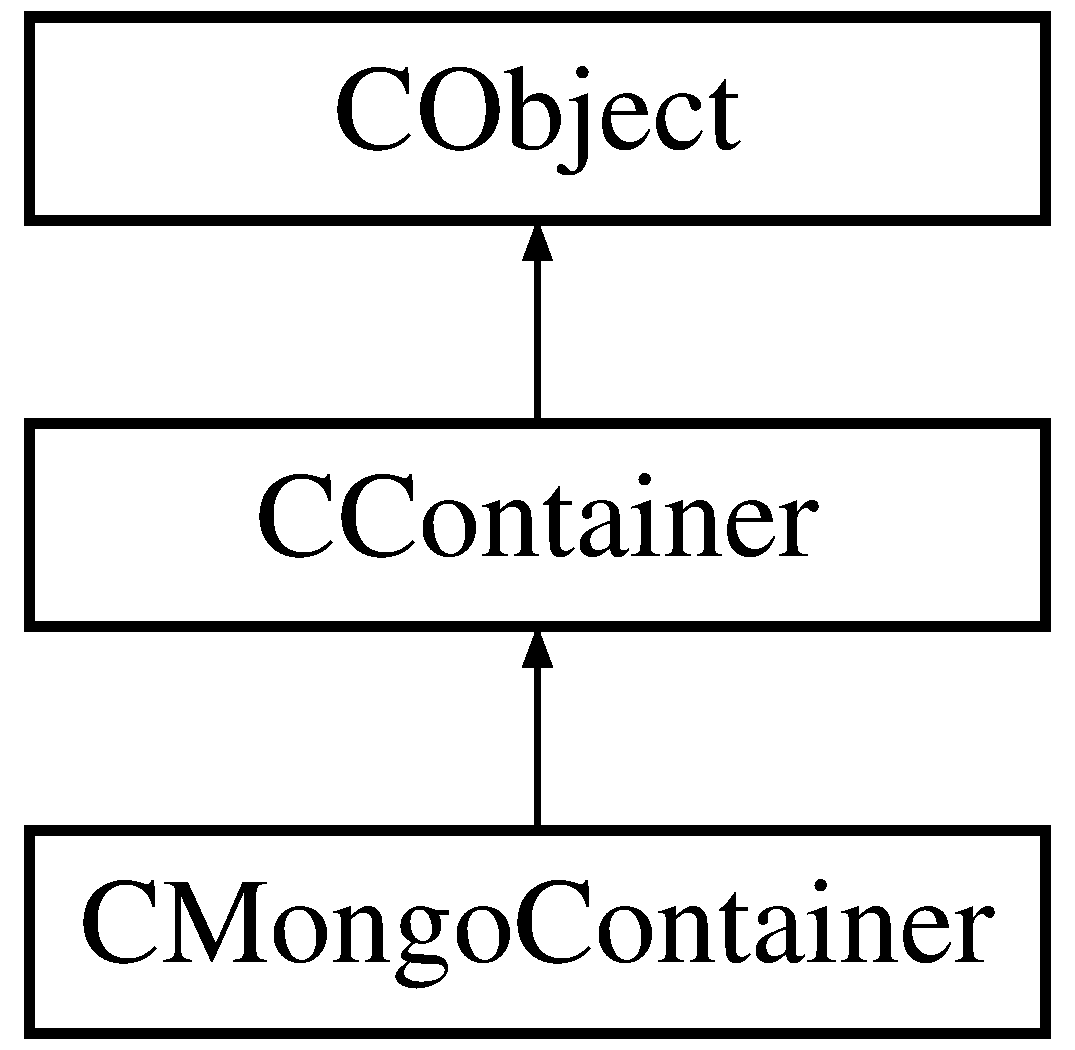
\includegraphics[height=4.000000cm]{class_c_mongo_container}
\end{center}
\end{figure}
\subsection*{Public Member Functions}
\begin{DoxyCompactItemize}
\item 
\hyperlink{class_c_mongo_container_abc325eae251667da577efdb45a7d3c17}{\-\_\-\-\_\-to\-String} ()
\item 
\hyperlink{class_c_mongo_container_a253978bb8e4d1e2613665d308de83e1e}{Container} (\$the\-Value=N\-U\-L\-L, \$get\-Old=F\-A\-L\-S\-E)
\item 
\hyperlink{class_c_mongo_container_a27a99b6ea891b226729bc6cb8426cac0}{Database} ()
\item 
\hyperlink{class_c_mongo_container_a077bdbf148dfa01f3798015906e4e70a}{Unserialise\-Data} (\&\$the\-Element)
\end{DoxyCompactItemize}
\subsection*{Protected Member Functions}
\begin{DoxyCompactItemize}
\item 
\hyperlink{class_c_mongo_container_a92cbcdba4f2b0bda2ae3eeb7a08d7ba2}{\-\_\-\-Commit} (\&\$the\-Object, \&\$the\-Identifier, \&\$the\-Modifiers)
\item 
\hyperlink{class_c_mongo_container_a61f469d1975834b22665392542620317}{\-\_\-\-Load} (\&\$the\-Identifier, \&\$the\-Modifiers)
\item 
\hyperlink{class_c_mongo_container_aa516a049efe0c9083e2f8c5b9f9076a4}{\-\_\-\-Delete} (\&\$the\-Identifier, \&\$the\-Modifiers)
\item 
\hyperlink{class_c_mongo_container_af592e4500a640190f374c18683af3b83}{\-\_\-\-Prepare\-Commit} (\&\$the\-Object, \&\$the\-Identifier, \&\$the\-Modifiers)
\item 
\hyperlink{class_c_mongo_container_a2c44e9229169abde420adf34045f5382}{\-\_\-\-Prepare\-Load} (\&\$the\-Identifier, \&\$the\-Modifiers)
\end{DoxyCompactItemize}
\subsection*{Additional Inherited Members}


\subsection{Member Function Documentation}
\hypertarget{class_c_mongo_container_abc325eae251667da577efdb45a7d3c17}{\index{C\-Mongo\-Container@{C\-Mongo\-Container}!\-\_\-\-\_\-to\-String@{\-\_\-\-\_\-to\-String}}
\index{\-\_\-\-\_\-to\-String@{\-\_\-\-\_\-to\-String}!CMongoContainer@{C\-Mongo\-Container}}
\subsubsection[{\-\_\-\-\_\-to\-String}]{\setlength{\rightskip}{0pt plus 5cm}C\-Mongo\-Container\-::\-\_\-\-\_\-to\-String (
\begin{DoxyParamCaption}
{}
\end{DoxyParamCaption}
)}}\label{class_c_mongo_container_abc325eae251667da577efdb45a7d3c17}
Return container name.

This method should return the current container's name.

In this class we return the collection name.

public \begin{DoxyReturn}{Returns}
string
\end{DoxyReturn}
\hyperlink{class_c_mongo_container_a253978bb8e4d1e2613665d308de83e1e}{Container()} 

Reimplemented from \hyperlink{class_c_container_aa1d6ed5052f55cdffcf6445968f203ed}{C\-Container}.

\hypertarget{class_c_mongo_container_a92cbcdba4f2b0bda2ae3eeb7a08d7ba2}{\index{C\-Mongo\-Container@{C\-Mongo\-Container}!\-\_\-\-Commit@{\-\_\-\-Commit}}
\index{\-\_\-\-Commit@{\-\_\-\-Commit}!CMongoContainer@{C\-Mongo\-Container}}
\subsubsection[{\-\_\-\-Commit}]{\setlength{\rightskip}{0pt plus 5cm}C\-Mongo\-Container\-::\-\_\-\-Commit (
\begin{DoxyParamCaption}
\item[{\&}]{\$the\-Object, }
\item[{\&}]{\$the\-Identifier, }
\item[{\&}]{\$the\-Modifiers}
\end{DoxyParamCaption}
)\hspace{0.3cm}{\ttfamily [protected]}}}\label{class_c_mongo_container_a92cbcdba4f2b0bda2ae3eeb7a08d7ba2}
Commit provided object.

We implement this method to handle Mongo\-Collection object stores, this method will store the object in the current container.

The method will check if the current container is a Mongo\-Collection, if this is not the case, it will raise an \hyperlink{}{exception}.

If the provided modifiers indicate a \hyperlink{}{modify} operation, the method will return the modified object, in all other cases the method will return the object identifier.


\begin{DoxyParams}[1]{Parameters}
reference & {\em \&\$the\-Object} & Object to commit. \\
\hline
reference & {\em \&\$the\-Identifier} & Object identifier. \\
\hline
reference & {\em \&\$the\-Modifiers} & Commit modifiers.\\
\hline
\end{DoxyParams}
protected \begin{DoxyReturn}{Returns}
mixed
\end{DoxyReturn}
\hyperlink{class_c_mongo_container_a253978bb8e4d1e2613665d308de83e1e}{Container()}

\begin{DoxySeeAlso}{See Also}
k\-F\-L\-A\-G\-\_\-\-P\-E\-R\-S\-I\-S\-T\-\_\-\-I\-N\-S\-E\-R\-T k\-F\-L\-A\-G\-\_\-\-P\-E\-R\-S\-I\-S\-T\-\_\-\-M\-O\-D\-I\-F\-Y 

k\-F\-L\-A\-G\-\_\-\-P\-E\-R\-S\-I\-S\-T\-\_\-\-R\-E\-P\-L\-A\-C\-E k\-F\-L\-A\-G\-\_\-\-P\-E\-R\-S\-I\-S\-T\-\_\-\-U\-P\-D\-A\-T\-E 
\end{DoxySeeAlso}


Reimplemented from \hyperlink{class_c_container_acbc85dd164615b31c9edfec93bcf27f9}{C\-Container}.



Reimplemented in \hyperlink{class_c_mongo_grid_container_a1dc8378e77df7c06afc2c733e2422482}{C\-Mongo\-Grid\-Container}.

\hypertarget{class_c_mongo_container_aa516a049efe0c9083e2f8c5b9f9076a4}{\index{C\-Mongo\-Container@{C\-Mongo\-Container}!\-\_\-\-Delete@{\-\_\-\-Delete}}
\index{\-\_\-\-Delete@{\-\_\-\-Delete}!CMongoContainer@{C\-Mongo\-Container}}
\subsubsection[{\-\_\-\-Delete}]{\setlength{\rightskip}{0pt plus 5cm}C\-Mongo\-Container\-::\-\_\-\-Delete (
\begin{DoxyParamCaption}
\item[{\&}]{\$the\-Identifier, }
\item[{\&}]{\$the\-Modifiers}
\end{DoxyParamCaption}
)\hspace{0.3cm}{\ttfamily [protected]}}}\label{class_c_mongo_container_aa516a049efe0c9083e2f8c5b9f9076a4}
Delete object.

We implement this method to handle Mongo\-Collection object stores, this method will remove the object from the current container.


\begin{DoxyParams}[1]{Parameters}
reference & {\em \&\$the\-Identifier} & Object identifier. \\
\hline
reference & {\em \&\$the\-Modifiers} & Load modifiers.\\
\hline
\end{DoxyParams}
protected \begin{DoxyReturn}{Returns}
mixed 
\end{DoxyReturn}


Reimplemented from \hyperlink{class_c_container_a20aac3eec154c2122f2c602bf5ce35fe}{C\-Container}.

\hypertarget{class_c_mongo_container_a61f469d1975834b22665392542620317}{\index{C\-Mongo\-Container@{C\-Mongo\-Container}!\-\_\-\-Load@{\-\_\-\-Load}}
\index{\-\_\-\-Load@{\-\_\-\-Load}!CMongoContainer@{C\-Mongo\-Container}}
\subsubsection[{\-\_\-\-Load}]{\setlength{\rightskip}{0pt plus 5cm}C\-Mongo\-Container\-::\-\_\-\-Load (
\begin{DoxyParamCaption}
\item[{\&}]{\$the\-Identifier, }
\item[{\&}]{\$the\-Modifiers}
\end{DoxyParamCaption}
)\hspace{0.3cm}{\ttfamily [protected]}}}\label{class_c_mongo_container_a61f469d1975834b22665392542620317}
Load object.

We implement this method to handle Mongo\-Collection object stores, this method will retrieve the object from the current container.

The \hyperlink{class_c_container_a48db96aa6bbf15d0bfc15725616b7154}{caller} will have resolved references andeventually extracted the identifier from the provided parameter.

If the provided parameter is an array, the method will assume it is a query; if not, the method will assume it is the value to match against the \hyperlink{}{local} identifier.

The method will use the {\itshape find\-One} method to retrieve the object.


\begin{DoxyParams}[1]{Parameters}
reference & {\em \&\$the\-Identifier} & Object identifier. \\
\hline
reference & {\em \&\$the\-Modifiers} & Load modifiers.\\
\hline
\end{DoxyParams}
protected \begin{DoxyReturn}{Returns}
mixed 
\end{DoxyReturn}


Reimplemented from \hyperlink{class_c_container_a865f140560991fa21a88b7fc8ff8f1f5}{C\-Container}.

\hypertarget{class_c_mongo_container_af592e4500a640190f374c18683af3b83}{\index{C\-Mongo\-Container@{C\-Mongo\-Container}!\-\_\-\-Prepare\-Commit@{\-\_\-\-Prepare\-Commit}}
\index{\-\_\-\-Prepare\-Commit@{\-\_\-\-Prepare\-Commit}!CMongoContainer@{C\-Mongo\-Container}}
\subsubsection[{\-\_\-\-Prepare\-Commit}]{\setlength{\rightskip}{0pt plus 5cm}C\-Mongo\-Container\-::\-\_\-\-Prepare\-Commit (
\begin{DoxyParamCaption}
\item[{\&}]{\$the\-Object, }
\item[{\&}]{\$the\-Identifier, }
\item[{\&}]{\$the\-Modifiers}
\end{DoxyParamCaption}
)\hspace{0.3cm}{\ttfamily [protected]}}}\label{class_c_mongo_container_af592e4500a640190f374c18683af3b83}
Prepare before a \hyperlink{class_c_mongo_container_a92cbcdba4f2b0bda2ae3eeb7a08d7ba2}{commit}.

We \hyperlink{class_c_container_a0dc47e54abc533cedf1c2c0f915d96b2}{overload} this method to handle the identifier\-: if provided, it means that that is to become the object's unique \hyperlink{}{identifier}; if not provided and the object has an \hyperlink{}{identifier}, we use that one.

We also raise an exception if the provided object is not either an array or an Array\-Object.


\begin{DoxyParams}[1]{Parameters}
reference & {\em \&\$the\-Object} & Object or data. \\
\hline
reference & {\em \&\$the\-Identifier} & Object identifier. \\
\hline
reference & {\em \&\$the\-Modifiers} & Commit modifiers.\\
\hline
\end{DoxyParams}
protected


\begin{DoxyExceptions}{Exceptions}
{\em \{@link} & \hyperlink{class_c_exception}{C\-Exception} \hyperlink{class_c_exception}{C\-Exception}\}\\
\hline
\end{DoxyExceptions}
\hyperlink{class_c_mongo_container_a253978bb8e4d1e2613665d308de83e1e}{Container()}

\begin{DoxySeeAlso}{See Also}
k\-F\-L\-A\-G\-\_\-\-S\-T\-A\-T\-E\-\_\-\-E\-N\-C\-O\-D\-E\-D 

k\-E\-R\-R\-O\-R\-\_\-\-O\-P\-T\-I\-O\-N\-\_\-\-M\-I\-S\-S\-I\-N\-G k\-E\-R\-R\-O\-R\-\_\-\-I\-N\-V\-A\-L\-I\-D\-\_\-\-P\-A\-R\-A\-M\-E\-T\-E\-R k\-E\-R\-R\-O\-R\-\_\-\-I\-N\-V\-A\-L\-I\-D\-\_\-\-S\-T\-A\-T\-E 
\end{DoxySeeAlso}


Reimplemented from \hyperlink{class_c_container_a0dc47e54abc533cedf1c2c0f915d96b2}{C\-Container}.



Reimplemented in \hyperlink{class_c_mongo_grid_container_a94715c26002c38020a8e4103d3075426}{C\-Mongo\-Grid\-Container}.

\hypertarget{class_c_mongo_container_a2c44e9229169abde420adf34045f5382}{\index{C\-Mongo\-Container@{C\-Mongo\-Container}!\-\_\-\-Prepare\-Load@{\-\_\-\-Prepare\-Load}}
\index{\-\_\-\-Prepare\-Load@{\-\_\-\-Prepare\-Load}!CMongoContainer@{C\-Mongo\-Container}}
\subsubsection[{\-\_\-\-Prepare\-Load}]{\setlength{\rightskip}{0pt plus 5cm}C\-Mongo\-Container\-::\-\_\-\-Prepare\-Load (
\begin{DoxyParamCaption}
\item[{\&}]{\$the\-Identifier, }
\item[{\&}]{\$the\-Modifiers}
\end{DoxyParamCaption}
)\hspace{0.3cm}{\ttfamily [protected]}}}\label{class_c_mongo_container_a2c44e9229169abde420adf34045f5382}
Prepare before a \hyperlink{class_c_mongo_container_a61f469d1975834b22665392542620317}{load}.

The duty of this method is to ensure that the parameters provided to the \hyperlink{class_c_mongo_container_a61f469d1975834b22665392542620317}{find} operation are valid.

In this class we \hyperlink{class_c_container_a1b84868c32fcfd3e11a9f6cc85fc461c}{overload} this method to handle identifiers provided as queries.


\begin{DoxyParams}[1]{Parameters}
reference & {\em \&\$the\-Identifier} & Object identifier. \\
\hline
reference & {\em \&\$the\-Modifiers} & Create modifiers.\\
\hline
\end{DoxyParams}
protected


\begin{DoxyExceptions}{Exceptions}
{\em \{@link} & \hyperlink{class_c_exception}{C\-Exception} \hyperlink{class_c_exception}{C\-Exception}\}\\
\hline
\end{DoxyExceptions}
\hyperlink{class_c_mongo_container_a253978bb8e4d1e2613665d308de83e1e}{Container()}  \hyperlink{class_c_mongo_container_a077bdbf148dfa01f3798015906e4e70a}{Unserialise\-Data()}

\begin{DoxySeeAlso}{See Also}
k\-F\-L\-A\-G\-\_\-\-S\-T\-A\-T\-E\-\_\-\-E\-N\-C\-O\-D\-E\-D 
\end{DoxySeeAlso}


Reimplemented from \hyperlink{class_c_container_a1b84868c32fcfd3e11a9f6cc85fc461c}{C\-Container}.

\hypertarget{class_c_mongo_container_a253978bb8e4d1e2613665d308de83e1e}{\index{C\-Mongo\-Container@{C\-Mongo\-Container}!Container@{Container}}
\index{Container@{Container}!CMongoContainer@{C\-Mongo\-Container}}
\subsubsection[{Container}]{\setlength{\rightskip}{0pt plus 5cm}C\-Mongo\-Container\-::\-Container (
\begin{DoxyParamCaption}
\item[{}]{\$the\-Value = {\ttfamily NULL}, }
\item[{}]{\$get\-Old = {\ttfamily FALSE}}
\end{DoxyParamCaption}
)}}\label{class_c_mongo_container_a253978bb8e4d1e2613665d308de83e1e}
Manage persistent container.

We \hyperlink{class_c_container_a7d10fa70dfa381cb95e66c265e2ca113}{overload} this method to ensure that the provided container is a Mongo\-Collection object.


\begin{DoxyParams}[1]{Parameters}
mixed & {\em \$the\-Value} & Persistent container or operation. \\
\hline
boolean & {\em \$get\-Old} & T\-R\-U\-E get old value.\\
\hline
\end{DoxyParams}
public \begin{DoxyReturn}{Returns}
mixed 
\end{DoxyReturn}


Reimplemented from \hyperlink{class_c_container_a7d10fa70dfa381cb95e66c265e2ca113}{C\-Container}.



Reimplemented in \hyperlink{class_c_mongo_grid_container_aafde59c8f7bf042d0e4f3a8d7bc87d90}{C\-Mongo\-Grid\-Container}.

\hypertarget{class_c_mongo_container_a27a99b6ea891b226729bc6cb8426cac0}{\index{C\-Mongo\-Container@{C\-Mongo\-Container}!Database@{Database}}
\index{Database@{Database}!CMongoContainer@{C\-Mongo\-Container}}
\subsubsection[{Database}]{\setlength{\rightskip}{0pt plus 5cm}C\-Mongo\-Container\-::\-Database (
\begin{DoxyParamCaption}
{}
\end{DoxyParamCaption}
)}}\label{class_c_mongo_container_a27a99b6ea891b226729bc6cb8426cac0}
Return database.

In this class we return the collection's database.

public \begin{DoxyReturn}{Returns}
mixed
\end{DoxyReturn}
\hyperlink{class_c_mongo_container_a253978bb8e4d1e2613665d308de83e1e}{Container()} 

Reimplemented from \hyperlink{class_c_container_a0d691b62d9b70b924e24a332931ce9d1}{C\-Container}.

\hypertarget{class_c_mongo_container_a077bdbf148dfa01f3798015906e4e70a}{\index{C\-Mongo\-Container@{C\-Mongo\-Container}!Unserialise\-Data@{Unserialise\-Data}}
\index{Unserialise\-Data@{Unserialise\-Data}!CMongoContainer@{C\-Mongo\-Container}}
\subsubsection[{Unserialise\-Data}]{\setlength{\rightskip}{0pt plus 5cm}C\-Mongo\-Container\-::\-Unserialise\-Data (
\begin{DoxyParamCaption}
\item[{\&}]{\$the\-Element}
\end{DoxyParamCaption}
)}}\label{class_c_mongo_container_a077bdbf148dfa01f3798015906e4e70a}
Unserialise provided data element.

We \hyperlink{class_c_container_a09d585e2a9809221a42d52d7520c9cbf}{implement} this method to convert all standard \hyperlink{class_c_data_type}{types} into custom Mongo data types.

In this class we parse the following types and \hyperlink{}{offsets}\-:


\begin{DoxyItemize}
\item {\itshape \hyperlink{class_c_data_type_mongo_id}{C\-Data\-Type\-Mongo\-Id} object or \hyperlink{}{k\-T\-Y\-P\-E\-\_\-\-Mongo\-Id} offset}\-: We return a Mongo\-Id object. 
\item {\itshape \hyperlink{class_c_data_type_mongo_code}{C\-Data\-Type\-Mongo\-Code} object or \hyperlink{}{k\-T\-Y\-P\-E\-\_\-\-Mongo\-Code} offset}\-: We return a Mongo\-Code object. 
\item {\itshape \hyperlink{class_c_data_type_stamp}{C\-Data\-Type\-Stamp} object or \hyperlink{}{k\-T\-Y\-P\-E\-\_\-\-S\-T\-A\-M\-P} offset}\-: We return a Mongo\-Date object. 
\item {\itshape \hyperlink{class_c_data_type_regex}{C\-Data\-Type\-Regex} object or \hyperlink{}{k\-T\-Y\-P\-E\-\_\-\-R\-E\-G\-E\-X} offset}\-: We return a Mongo\-Regex object. 
\item {\itshape \hyperlink{class_c_data_type_int32}{C\-Data\-Type\-Int32} object or \hyperlink{}{k\-T\-Y\-P\-E\-\_\-\-I\-N\-T32} offset}\-: We return a Mongo\-Int32 object. 
\item {\itshape \hyperlink{class_c_data_type_int64}{C\-Data\-Type\-Int64} object or \hyperlink{}{k\-T\-Y\-P\-E\-\_\-\-I\-N\-T64} offset}\-: We return a Mongo\-Int64 object. 
\item {\itshape \hyperlink{class_c_data_type_binary}{C\-Data\-Type\-Binary} object or \hyperlink{}{k\-T\-Y\-P\-E\-\_\-\-B\-I\-N\-A\-R\-Y} offset}\-: We return a Mongo\-Bin\-Data object. 
\end{DoxyItemize}


\begin{DoxyParams}[1]{Parameters}
reference & {\em \&\$the\-Element} & Element to encode.\\
\hline
\end{DoxyParams}
public 

Reimplemented from \hyperlink{class_c_container_a09d585e2a9809221a42d52d7520c9cbf}{C\-Container}.



The documentation for this class was generated from the following file\-:\begin{DoxyCompactItemize}
\item 
/\-Library/\-Web\-Server/\-Library/wrapper/classes/C\-Mongo\-Container.\-php\end{DoxyCompactItemize}

\hypertarget{class_c_mongo_data_wrapper}{\section{C\-Mongo\-Data\-Wrapper Class Reference}
\label{class_c_mongo_data_wrapper}\index{C\-Mongo\-Data\-Wrapper@{C\-Mongo\-Data\-Wrapper}}
}
Inheritance diagram for C\-Mongo\-Data\-Wrapper\-:\begin{figure}[H]
\begin{center}
\leavevmode
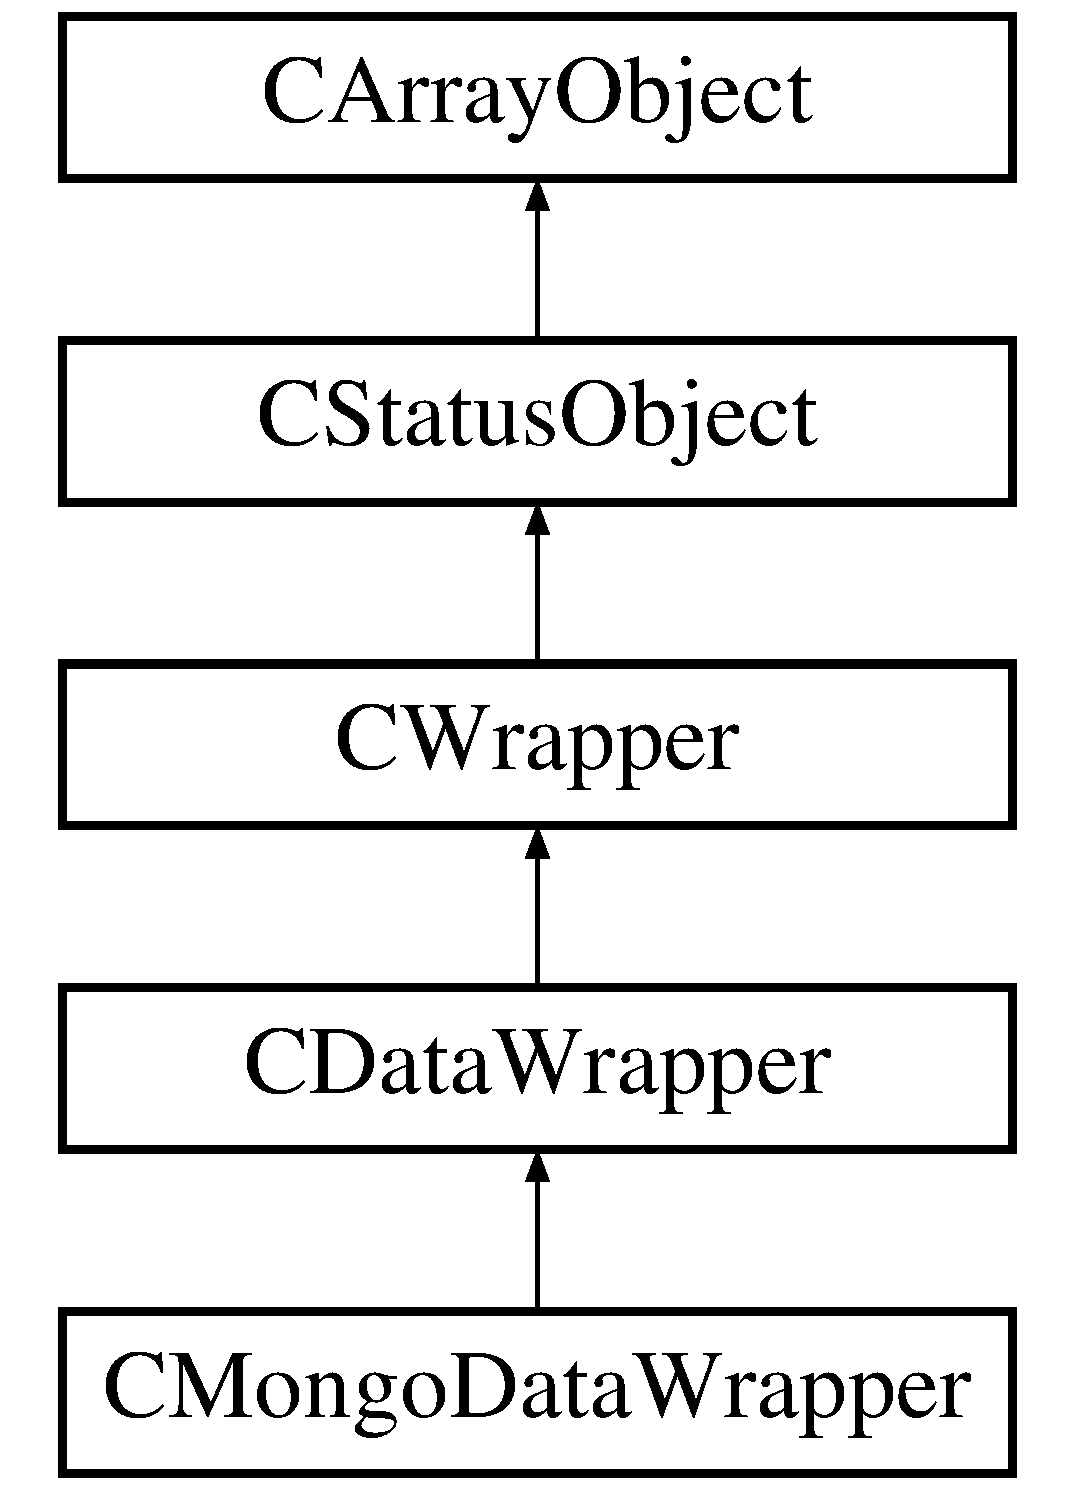
\includegraphics[height=6.000000cm]{class_c_mongo_data_wrapper}
\end{center}
\end{figure}
\subsection*{Protected Member Functions}
\begin{DoxyCompactItemize}
\item 
\hyperlink{class_c_mongo_data_wrapper_a33ff97c26b97d00a67f97d41f67ce47b}{\-\_\-\-Init\-Resources} ()
\item 
\hyperlink{class_c_mongo_data_wrapper_a8ac2f23cfc78f3fba6b256718ed2d105}{\-\_\-\-Parse\-Request} ()
\item 
\hyperlink{class_c_mongo_data_wrapper_abbc0d41394dda4a27eefa8481065749a}{\-\_\-\-Format\-Request} ()
\item 
\hyperlink{class_c_mongo_data_wrapper_a3d06376cb588e5c26751bff3f0083ef5}{\-\_\-\-Validate\-Request} ()
\item 
\hyperlink{class_c_mongo_data_wrapper_adb77016dd91f53f6e5d74a7390020c4d}{\-\_\-\-Parse\-No\-Response} ()
\item 
\hyperlink{class_c_mongo_data_wrapper_a15b44586fe5de968efb0edbe96f3da60}{\-\_\-\-Format\-Database} ()
\item 
\hyperlink{class_c_mongo_data_wrapper_a117d32ff4a01a54a7ff6203ba0ca66b7}{\-\_\-\-Format\-Container} ()
\item 
\hyperlink{class_c_mongo_data_wrapper_a807db77c3c4f7708e86873a0447b83ff}{\-\_\-\-Format\-Query} ()
\item 
\hyperlink{class_c_mongo_data_wrapper_a2642638da121e471c7ea1fbb61f6f3ef}{\-\_\-\-Format\-Object} ()
\item 
\hyperlink{class_c_mongo_data_wrapper_a406b81115b5f3957e6d40ee49ae85a13}{\-\_\-\-Validate\-Operation} ()
\item 
\hyperlink{class_c_mongo_data_wrapper_a9bb974219920f005b1cdba39793b84d5}{\-\_\-\-Validate\-Object} ()
\item 
\hyperlink{class_c_mongo_data_wrapper_aa2ae2292a247d94c9b1dfa13d9a4fb85}{\-\_\-\-Validate\-Query} ()
\item 
\hyperlink{class_c_mongo_data_wrapper_a811af7e7574a459bc56afa3afa99e1a8}{\-\_\-\-Handle\-Request} ()
\item 
\hyperlink{class_c_mongo_data_wrapper_a1ca51f95510a94bf26e004ef2e8e8d37}{\-\_\-\-Handle\-\_\-\-List\-Op} (\&\$the\-List)
\item 
\hyperlink{class_c_mongo_data_wrapper_a226970d3cfb96f8e85e46d3943c25089}{\-\_\-\-Handle\-\_\-\-Get\-Object\-By\-Reference} ()
\item 
\hyperlink{class_c_mongo_data_wrapper_ae7cc52809c8b6cea94c84d5f64a4308b}{\-\_\-\-Handle\-\_\-\-Count} ()
\item 
\hyperlink{class_c_mongo_data_wrapper_a3b9896d121c899aa3dd9f5e56e44c874}{\-\_\-\-Handle\-\_\-\-Get\-One} ()
\item 
\hyperlink{class_c_mongo_data_wrapper_a157a45bd4a2da43bd05d62b22faf3dc6}{\-\_\-\-Handle\-\_\-\-Get} ()
\item 
\hyperlink{class_c_mongo_data_wrapper_a8b9654ce201a453a76a5075bd7ce8a38}{\-\_\-\-Handle\-\_\-\-Match} ()
\item 
\hyperlink{class_c_mongo_data_wrapper_a3b59e4f2efbe64568c500756a170af29}{\-\_\-\-Handle\-\_\-\-Set} ()
\item 
\hyperlink{class_c_mongo_data_wrapper_adc1ef56d8c5fe9dbab74a821f38fe62c}{\-\_\-\-Handle\-\_\-\-Insert} ()
\item 
\hyperlink{class_c_mongo_data_wrapper_a5618d7ca3fe124a76bb62360525b01be}{\-\_\-\-Handle\-\_\-\-Batch\-Insert} ()
\item 
\hyperlink{class_c_mongo_data_wrapper_a271b356a503ae0ab4a67610f808a6a9a}{\-\_\-\-Handle\-\_\-\-Update} ()
\item 
\hyperlink{class_c_mongo_data_wrapper_a1b61fb28b8917a53948b02194902eb34}{\-\_\-\-Handle\-\_\-\-Modify} ()
\item 
\hyperlink{class_c_mongo_data_wrapper_aaed227073838fb79b344e3d07a3152e8}{\-\_\-\-Handle\-\_\-\-Delete} ()
\item 
\hyperlink{class_c_mongo_data_wrapper_ac154306e6919de8316ddf45fc8d619f3}{\-\_\-\-Handle\-Options} (\&\$the\-Result, \$the\-Options)
\end{DoxyCompactItemize}


\subsection{Member Function Documentation}
\hypertarget{class_c_mongo_data_wrapper_a117d32ff4a01a54a7ff6203ba0ca66b7}{\index{C\-Mongo\-Data\-Wrapper@{C\-Mongo\-Data\-Wrapper}!\-\_\-\-Format\-Container@{\-\_\-\-Format\-Container}}
\index{\-\_\-\-Format\-Container@{\-\_\-\-Format\-Container}!CMongoDataWrapper@{C\-Mongo\-Data\-Wrapper}}
\subsubsection[{\-\_\-\-Format\-Container}]{\setlength{\rightskip}{0pt plus 5cm}C\-Mongo\-Data\-Wrapper\-::\-\_\-\-Format\-Container (
\begin{DoxyParamCaption}
{}
\end{DoxyParamCaption}
)\hspace{0.3cm}{\ttfamily [protected]}}}\label{class_c_mongo_data_wrapper_a117d32ff4a01a54a7ff6203ba0ca66b7}
Format container.

This method will format the request container.

In this class we set the request container to a Mongo\-Collection object.

protected \hypertarget{class_c_mongo_data_wrapper_a15b44586fe5de968efb0edbe96f3da60}{\index{C\-Mongo\-Data\-Wrapper@{C\-Mongo\-Data\-Wrapper}!\-\_\-\-Format\-Database@{\-\_\-\-Format\-Database}}
\index{\-\_\-\-Format\-Database@{\-\_\-\-Format\-Database}!CMongoDataWrapper@{C\-Mongo\-Data\-Wrapper}}
\subsubsection[{\-\_\-\-Format\-Database}]{\setlength{\rightskip}{0pt plus 5cm}C\-Mongo\-Data\-Wrapper\-::\-\_\-\-Format\-Database (
\begin{DoxyParamCaption}
{}
\end{DoxyParamCaption}
)\hspace{0.3cm}{\ttfamily [protected]}}}\label{class_c_mongo_data_wrapper_a15b44586fe5de968efb0edbe96f3da60}
Format database.

This method will format the request database.

In this class we set the database to a Mongo\-D\-B object.

protected \hypertarget{class_c_mongo_data_wrapper_a2642638da121e471c7ea1fbb61f6f3ef}{\index{C\-Mongo\-Data\-Wrapper@{C\-Mongo\-Data\-Wrapper}!\-\_\-\-Format\-Object@{\-\_\-\-Format\-Object}}
\index{\-\_\-\-Format\-Object@{\-\_\-\-Format\-Object}!CMongoDataWrapper@{C\-Mongo\-Data\-Wrapper}}
\subsubsection[{\-\_\-\-Format\-Object}]{\setlength{\rightskip}{0pt plus 5cm}C\-Mongo\-Data\-Wrapper\-::\-\_\-\-Format\-Object (
\begin{DoxyParamCaption}
{}
\end{DoxyParamCaption}
)\hspace{0.3cm}{\ttfamily [protected]}}}\label{class_c_mongo_data_wrapper_a2642638da121e471c7ea1fbb61f6f3ef}
Format object.

This method will format the request object.

In this class we resolve the Mongo native types.

protected 

Reimplemented from \hyperlink{class_c_data_wrapper_addefb7bd419de62bfebedc21abbdad7e}{C\-Data\-Wrapper}.

\hypertarget{class_c_mongo_data_wrapper_a807db77c3c4f7708e86873a0447b83ff}{\index{C\-Mongo\-Data\-Wrapper@{C\-Mongo\-Data\-Wrapper}!\-\_\-\-Format\-Query@{\-\_\-\-Format\-Query}}
\index{\-\_\-\-Format\-Query@{\-\_\-\-Format\-Query}!CMongoDataWrapper@{C\-Mongo\-Data\-Wrapper}}
\subsubsection[{\-\_\-\-Format\-Query}]{\setlength{\rightskip}{0pt plus 5cm}C\-Mongo\-Data\-Wrapper\-::\-\_\-\-Format\-Query (
\begin{DoxyParamCaption}
{}
\end{DoxyParamCaption}
)\hspace{0.3cm}{\ttfamily [protected]}}}\label{class_c_mongo_data_wrapper_a807db77c3c4f7708e86873a0447b83ff}
Format query.

This method will format the request query.

In this class we set the query to a \hyperlink{class_c_mongo_query}{C\-Mongo\-Query} object.

protected 

Reimplemented from \hyperlink{class_c_data_wrapper_a0c3054fcf3716d638922cd581d5c706e}{C\-Data\-Wrapper}.

\hypertarget{class_c_mongo_data_wrapper_abbc0d41394dda4a27eefa8481065749a}{\index{C\-Mongo\-Data\-Wrapper@{C\-Mongo\-Data\-Wrapper}!\-\_\-\-Format\-Request@{\-\_\-\-Format\-Request}}
\index{\-\_\-\-Format\-Request@{\-\_\-\-Format\-Request}!CMongoDataWrapper@{C\-Mongo\-Data\-Wrapper}}
\subsubsection[{\-\_\-\-Format\-Request}]{\setlength{\rightskip}{0pt plus 5cm}C\-Mongo\-Data\-Wrapper\-::\-\_\-\-Format\-Request (
\begin{DoxyParamCaption}
{}
\end{DoxyParamCaption}
)\hspace{0.3cm}{\ttfamily [protected]}}}\label{class_c_mongo_data_wrapper_abbc0d41394dda4a27eefa8481065749a}
Format request.

This method should perform any needed formatting before the request will be handled.

In this class we handle the parameters to be decoded

protected 

Reimplemented from \hyperlink{class_c_data_wrapper_ab46c0e9797e8636ca1c9d535b377b90a}{C\-Data\-Wrapper}.



Reimplemented in \hyperlink{class_c_warehouse_wrapper_a4bd0282949f52ce148b60218c48ddde5}{C\-Warehouse\-Wrapper}.

\hypertarget{class_c_mongo_data_wrapper_a5618d7ca3fe124a76bb62360525b01be}{\index{C\-Mongo\-Data\-Wrapper@{C\-Mongo\-Data\-Wrapper}!\-\_\-\-Handle\-\_\-\-Batch\-Insert@{\-\_\-\-Handle\-\_\-\-Batch\-Insert}}
\index{\-\_\-\-Handle\-\_\-\-Batch\-Insert@{\-\_\-\-Handle\-\_\-\-Batch\-Insert}!CMongoDataWrapper@{C\-Mongo\-Data\-Wrapper}}
\subsubsection[{\-\_\-\-Handle\-\_\-\-Batch\-Insert}]{\setlength{\rightskip}{0pt plus 5cm}C\-Mongo\-Data\-Wrapper\-::\-\_\-\-Handle\-\_\-\-Batch\-Insert (
\begin{DoxyParamCaption}
{}
\end{DoxyParamCaption}
)\hspace{0.3cm}{\ttfamily [protected]}}}\label{class_c_mongo_data_wrapper_a5618d7ca3fe124a76bb62360525b01be}
Handle \hyperlink{}{batch} Insert request.

This method will handle the \hyperlink{}{k\-A\-P\-I\-\_\-\-O\-P\-\_\-\-B\-A\-T\-C\-H\-\_\-\-I\-N\-S\-E\-R\-T} request, which will insert the provided list of objects.

protected \hypertarget{class_c_mongo_data_wrapper_ae7cc52809c8b6cea94c84d5f64a4308b}{\index{C\-Mongo\-Data\-Wrapper@{C\-Mongo\-Data\-Wrapper}!\-\_\-\-Handle\-\_\-\-Count@{\-\_\-\-Handle\-\_\-\-Count}}
\index{\-\_\-\-Handle\-\_\-\-Count@{\-\_\-\-Handle\-\_\-\-Count}!CMongoDataWrapper@{C\-Mongo\-Data\-Wrapper}}
\subsubsection[{\-\_\-\-Handle\-\_\-\-Count}]{\setlength{\rightskip}{0pt plus 5cm}C\-Mongo\-Data\-Wrapper\-::\-\_\-\-Handle\-\_\-\-Count (
\begin{DoxyParamCaption}
{}
\end{DoxyParamCaption}
)\hspace{0.3cm}{\ttfamily [protected]}}}\label{class_c_mongo_data_wrapper_ae7cc52809c8b6cea94c84d5f64a4308b}
Handle \hyperlink{}{C\-O\-U\-N\-T} request.

This method will handle the \hyperlink{}{k\-A\-P\-I\-\_\-\-O\-P\-\_\-\-C\-O\-U\-N\-T} request, which returns the total count of a Mongo query.

protected \hypertarget{class_c_mongo_data_wrapper_aaed227073838fb79b344e3d07a3152e8}{\index{C\-Mongo\-Data\-Wrapper@{C\-Mongo\-Data\-Wrapper}!\-\_\-\-Handle\-\_\-\-Delete@{\-\_\-\-Handle\-\_\-\-Delete}}
\index{\-\_\-\-Handle\-\_\-\-Delete@{\-\_\-\-Handle\-\_\-\-Delete}!CMongoDataWrapper@{C\-Mongo\-Data\-Wrapper}}
\subsubsection[{\-\_\-\-Handle\-\_\-\-Delete}]{\setlength{\rightskip}{0pt plus 5cm}C\-Mongo\-Data\-Wrapper\-::\-\_\-\-Handle\-\_\-\-Delete (
\begin{DoxyParamCaption}
{}
\end{DoxyParamCaption}
)\hspace{0.3cm}{\ttfamily [protected]}}}\label{class_c_mongo_data_wrapper_aaed227073838fb79b344e3d07a3152e8}
Handle \hyperlink{}{Delete} request.

This method will handle the \hyperlink{}{k\-A\-P\-I\-\_\-\-O\-P\-\_\-\-D\-E\-L} request, whichwill delete all objects matching the provided filter.

The method expects the {\itshape just\-One} parameter in the provided \hyperlink{}{options}, if not provided, it will default to {\itshape F\-A\-L\-S\-E}.

protected \hypertarget{class_c_mongo_data_wrapper_a157a45bd4a2da43bd05d62b22faf3dc6}{\index{C\-Mongo\-Data\-Wrapper@{C\-Mongo\-Data\-Wrapper}!\-\_\-\-Handle\-\_\-\-Get@{\-\_\-\-Handle\-\_\-\-Get}}
\index{\-\_\-\-Handle\-\_\-\-Get@{\-\_\-\-Handle\-\_\-\-Get}!CMongoDataWrapper@{C\-Mongo\-Data\-Wrapper}}
\subsubsection[{\-\_\-\-Handle\-\_\-\-Get}]{\setlength{\rightskip}{0pt plus 5cm}C\-Mongo\-Data\-Wrapper\-::\-\_\-\-Handle\-\_\-\-Get (
\begin{DoxyParamCaption}
{}
\end{DoxyParamCaption}
)\hspace{0.3cm}{\ttfamily [protected]}}}\label{class_c_mongo_data_wrapper_a157a45bd4a2da43bd05d62b22faf3dc6}
Handle \hyperlink{}{Get} request.

This method will handle the \hyperlink{}{k\-A\-P\-I\-\_\-\-O\-P\-\_\-\-G\-E\-T} request, which corresponds to the find Mongo query.

protected \hypertarget{class_c_mongo_data_wrapper_a226970d3cfb96f8e85e46d3943c25089}{\index{C\-Mongo\-Data\-Wrapper@{C\-Mongo\-Data\-Wrapper}!\-\_\-\-Handle\-\_\-\-Get\-Object\-By\-Reference@{\-\_\-\-Handle\-\_\-\-Get\-Object\-By\-Reference}}
\index{\-\_\-\-Handle\-\_\-\-Get\-Object\-By\-Reference@{\-\_\-\-Handle\-\_\-\-Get\-Object\-By\-Reference}!CMongoDataWrapper@{C\-Mongo\-Data\-Wrapper}}
\subsubsection[{\-\_\-\-Handle\-\_\-\-Get\-Object\-By\-Reference}]{\setlength{\rightskip}{0pt plus 5cm}C\-Mongo\-Data\-Wrapper\-::\-\_\-\-Handle\-\_\-\-Get\-Object\-By\-Reference (
\begin{DoxyParamCaption}
{}
\end{DoxyParamCaption}
)\hspace{0.3cm}{\ttfamily [protected]}}}\label{class_c_mongo_data_wrapper_a226970d3cfb96f8e85e46d3943c25089}
Handle \hyperlink{}{Get\-Object\-By\-Reference} request.

This method will handle the \hyperlink{}{k\-A\-P\-I\-\_\-\-O\-P\-\_\-\-G\-E\-T\-\_\-\-O\-B\-J\-E\-C\-T\-\_\-\-R\-E\-F} request, which returns an object corresponding to the object \hyperlink{}{reference} provided in the \hyperlink{}{object} parameter.

protected \hypertarget{class_c_mongo_data_wrapper_a3b9896d121c899aa3dd9f5e56e44c874}{\index{C\-Mongo\-Data\-Wrapper@{C\-Mongo\-Data\-Wrapper}!\-\_\-\-Handle\-\_\-\-Get\-One@{\-\_\-\-Handle\-\_\-\-Get\-One}}
\index{\-\_\-\-Handle\-\_\-\-Get\-One@{\-\_\-\-Handle\-\_\-\-Get\-One}!CMongoDataWrapper@{C\-Mongo\-Data\-Wrapper}}
\subsubsection[{\-\_\-\-Handle\-\_\-\-Get\-One}]{\setlength{\rightskip}{0pt plus 5cm}C\-Mongo\-Data\-Wrapper\-::\-\_\-\-Handle\-\_\-\-Get\-One (
\begin{DoxyParamCaption}
{}
\end{DoxyParamCaption}
)\hspace{0.3cm}{\ttfamily [protected]}}}\label{class_c_mongo_data_wrapper_a3b9896d121c899aa3dd9f5e56e44c874}
Handle \hyperlink{}{Get\-One} request.

This method will handle the \hyperlink{}{k\-A\-P\-I\-\_\-\-O\-P\-\_\-\-G\-E\-T\-\_\-\-O\-N\-E} request, which corresponds to the find\-One Mongo query.

protected \hypertarget{class_c_mongo_data_wrapper_adc1ef56d8c5fe9dbab74a821f38fe62c}{\index{C\-Mongo\-Data\-Wrapper@{C\-Mongo\-Data\-Wrapper}!\-\_\-\-Handle\-\_\-\-Insert@{\-\_\-\-Handle\-\_\-\-Insert}}
\index{\-\_\-\-Handle\-\_\-\-Insert@{\-\_\-\-Handle\-\_\-\-Insert}!CMongoDataWrapper@{C\-Mongo\-Data\-Wrapper}}
\subsubsection[{\-\_\-\-Handle\-\_\-\-Insert}]{\setlength{\rightskip}{0pt plus 5cm}C\-Mongo\-Data\-Wrapper\-::\-\_\-\-Handle\-\_\-\-Insert (
\begin{DoxyParamCaption}
{}
\end{DoxyParamCaption}
)\hspace{0.3cm}{\ttfamily [protected]}}}\label{class_c_mongo_data_wrapper_adc1ef56d8c5fe9dbab74a821f38fe62c}
Handle \hyperlink{}{Insert} request.

This method will handle the \hyperlink{}{k\-A\-P\-I\-\_\-\-O\-P\-\_\-\-I\-N\-S\-E\-R\-T} request, which will insert the provided object.

protected \hypertarget{class_c_mongo_data_wrapper_a1ca51f95510a94bf26e004ef2e8e8d37}{\index{C\-Mongo\-Data\-Wrapper@{C\-Mongo\-Data\-Wrapper}!\-\_\-\-Handle\-\_\-\-List\-Op@{\-\_\-\-Handle\-\_\-\-List\-Op}}
\index{\-\_\-\-Handle\-\_\-\-List\-Op@{\-\_\-\-Handle\-\_\-\-List\-Op}!CMongoDataWrapper@{C\-Mongo\-Data\-Wrapper}}
\subsubsection[{\-\_\-\-Handle\-\_\-\-List\-Op}]{\setlength{\rightskip}{0pt plus 5cm}C\-Mongo\-Data\-Wrapper\-::\-\_\-\-Handle\-\_\-\-List\-Op (
\begin{DoxyParamCaption}
\item[{\&}]{\$the\-List}
\end{DoxyParamCaption}
)\hspace{0.3cm}{\ttfamily [protected]}}}\label{class_c_mongo_data_wrapper_a1ca51f95510a94bf26e004ef2e8e8d37}
Handle \hyperlink{}{list} operations request.

This method will handle the \hyperlink{}{k\-A\-P\-I\-\_\-\-O\-P\-\_\-\-H\-E\-L\-P} request, which should return the list of supported operations.


\begin{DoxyParams}[1]{Parameters}
reference & {\em \$the\-List} & Receives operations list.\\
\hline
\end{DoxyParams}
protected 

Reimplemented from \hyperlink{class_c_data_wrapper_afc7251c3aad9141599372d6b94904498}{C\-Data\-Wrapper}.



Reimplemented in \hyperlink{class_c_warehouse_wrapper_a9800cf5ca4bb22cd96a94ef542010adf}{C\-Warehouse\-Wrapper}.

\hypertarget{class_c_mongo_data_wrapper_a8b9654ce201a453a76a5075bd7ce8a38}{\index{C\-Mongo\-Data\-Wrapper@{C\-Mongo\-Data\-Wrapper}!\-\_\-\-Handle\-\_\-\-Match@{\-\_\-\-Handle\-\_\-\-Match}}
\index{\-\_\-\-Handle\-\_\-\-Match@{\-\_\-\-Handle\-\_\-\-Match}!CMongoDataWrapper@{C\-Mongo\-Data\-Wrapper}}
\subsubsection[{\-\_\-\-Handle\-\_\-\-Match}]{\setlength{\rightskip}{0pt plus 5cm}C\-Mongo\-Data\-Wrapper\-::\-\_\-\-Handle\-\_\-\-Match (
\begin{DoxyParamCaption}
{}
\end{DoxyParamCaption}
)\hspace{0.3cm}{\ttfamily [protected]}}}\label{class_c_mongo_data_wrapper_a8b9654ce201a453a76a5075bd7ce8a38}
Handle \hyperlink{}{Get} request.

This method will handle the \hyperlink{}{k\-A\-P\-I\-\_\-\-O\-P\-\_\-\-G\-E\-T} request, which corresponds to the find Mongo query.

protected \hypertarget{class_c_mongo_data_wrapper_a1b61fb28b8917a53948b02194902eb34}{\index{C\-Mongo\-Data\-Wrapper@{C\-Mongo\-Data\-Wrapper}!\-\_\-\-Handle\-\_\-\-Modify@{\-\_\-\-Handle\-\_\-\-Modify}}
\index{\-\_\-\-Handle\-\_\-\-Modify@{\-\_\-\-Handle\-\_\-\-Modify}!CMongoDataWrapper@{C\-Mongo\-Data\-Wrapper}}
\subsubsection[{\-\_\-\-Handle\-\_\-\-Modify}]{\setlength{\rightskip}{0pt plus 5cm}C\-Mongo\-Data\-Wrapper\-::\-\_\-\-Handle\-\_\-\-Modify (
\begin{DoxyParamCaption}
{}
\end{DoxyParamCaption}
)\hspace{0.3cm}{\ttfamily [protected]}}}\label{class_c_mongo_data_wrapper_a1b61fb28b8917a53948b02194902eb34}
Handle \hyperlink{}{Modify} request.

This method will handle the \hyperlink{}{k\-A\-P\-I\-\_\-\-O\-P\-\_\-\-M\-O\-D\-I\-F\-Y} request, which will update the provided object.

The data provided in the \hyperlink{}{object} parameter will be scanned and all {\itshape N\-U\-L\-L} values will be set in the {\itshape \$unset} array and the non {\itshape N\-U\-L\-L} values in the {\itshape \$set} array.

protected \hypertarget{class_c_mongo_data_wrapper_a3b59e4f2efbe64568c500756a170af29}{\index{C\-Mongo\-Data\-Wrapper@{C\-Mongo\-Data\-Wrapper}!\-\_\-\-Handle\-\_\-\-Set@{\-\_\-\-Handle\-\_\-\-Set}}
\index{\-\_\-\-Handle\-\_\-\-Set@{\-\_\-\-Handle\-\_\-\-Set}!CMongoDataWrapper@{C\-Mongo\-Data\-Wrapper}}
\subsubsection[{\-\_\-\-Handle\-\_\-\-Set}]{\setlength{\rightskip}{0pt plus 5cm}C\-Mongo\-Data\-Wrapper\-::\-\_\-\-Handle\-\_\-\-Set (
\begin{DoxyParamCaption}
{}
\end{DoxyParamCaption}
)\hspace{0.3cm}{\ttfamily [protected]}}}\label{class_c_mongo_data_wrapper_a3b59e4f2efbe64568c500756a170af29}
Handle \hyperlink{}{Set} request.

This method will handle the \hyperlink{}{k\-A\-P\-I\-\_\-\-O\-P\-\_\-\-S\-E\-T} request, which will insert/update the provided object.

protected \hypertarget{class_c_mongo_data_wrapper_a271b356a503ae0ab4a67610f808a6a9a}{\index{C\-Mongo\-Data\-Wrapper@{C\-Mongo\-Data\-Wrapper}!\-\_\-\-Handle\-\_\-\-Update@{\-\_\-\-Handle\-\_\-\-Update}}
\index{\-\_\-\-Handle\-\_\-\-Update@{\-\_\-\-Handle\-\_\-\-Update}!CMongoDataWrapper@{C\-Mongo\-Data\-Wrapper}}
\subsubsection[{\-\_\-\-Handle\-\_\-\-Update}]{\setlength{\rightskip}{0pt plus 5cm}C\-Mongo\-Data\-Wrapper\-::\-\_\-\-Handle\-\_\-\-Update (
\begin{DoxyParamCaption}
{}
\end{DoxyParamCaption}
)\hspace{0.3cm}{\ttfamily [protected]}}}\label{class_c_mongo_data_wrapper_a271b356a503ae0ab4a67610f808a6a9a}
Handle \hyperlink{}{Update} request.

This method will handle the \hyperlink{}{k\-A\-P\-I\-\_\-\-O\-P\-\_\-\-U\-P\-D\-A\-T\-E} request, which will update the provided object.

protected \hypertarget{class_c_mongo_data_wrapper_ac154306e6919de8316ddf45fc8d619f3}{\index{C\-Mongo\-Data\-Wrapper@{C\-Mongo\-Data\-Wrapper}!\-\_\-\-Handle\-Options@{\-\_\-\-Handle\-Options}}
\index{\-\_\-\-Handle\-Options@{\-\_\-\-Handle\-Options}!CMongoDataWrapper@{C\-Mongo\-Data\-Wrapper}}
\subsubsection[{\-\_\-\-Handle\-Options}]{\setlength{\rightskip}{0pt plus 5cm}C\-Mongo\-Data\-Wrapper\-::\-\_\-\-Handle\-Options (
\begin{DoxyParamCaption}
\item[{\&}]{\$the\-Result, }
\item[{}]{\$the\-Options}
\end{DoxyParamCaption}
)\hspace{0.3cm}{\ttfamily [protected]}}}\label{class_c_mongo_data_wrapper_ac154306e6919de8316ddf45fc8d619f3}
Handle options.

This method will be called before serialising the result if \hyperlink{}{options} are provided in the request.

In this class we don't do anything, derived classes should handle specific elements.


\begin{DoxyParams}[1]{Parameters}
reference & {\em \&\$the\-Result} & Results list. \\
\hline
array & {\em \$the\-Options} & Key/value options list.\\
\hline
\end{DoxyParams}
protected \hypertarget{class_c_mongo_data_wrapper_a811af7e7574a459bc56afa3afa99e1a8}{\index{C\-Mongo\-Data\-Wrapper@{C\-Mongo\-Data\-Wrapper}!\-\_\-\-Handle\-Request@{\-\_\-\-Handle\-Request}}
\index{\-\_\-\-Handle\-Request@{\-\_\-\-Handle\-Request}!CMongoDataWrapper@{C\-Mongo\-Data\-Wrapper}}
\subsubsection[{\-\_\-\-Handle\-Request}]{\setlength{\rightskip}{0pt plus 5cm}C\-Mongo\-Data\-Wrapper\-::\-\_\-\-Handle\-Request (
\begin{DoxyParamCaption}
{}
\end{DoxyParamCaption}
)\hspace{0.3cm}{\ttfamily [protected]}}}\label{class_c_mongo_data_wrapper_a811af7e7574a459bc56afa3afa99e1a8}
Handle request.

This method will handle the request.

protected 

Reimplemented from \hyperlink{class_c_wrapper_a12c1dd1f1d1cf0ae889cc19ff17ced0e}{C\-Wrapper}.



Reimplemented in \hyperlink{class_c_warehouse_wrapper_a4b909b5b4aba967200ff72e3e6924b5e}{C\-Warehouse\-Wrapper}.

\hypertarget{class_c_mongo_data_wrapper_a33ff97c26b97d00a67f97d41f67ce47b}{\index{C\-Mongo\-Data\-Wrapper@{C\-Mongo\-Data\-Wrapper}!\-\_\-\-Init\-Resources@{\-\_\-\-Init\-Resources}}
\index{\-\_\-\-Init\-Resources@{\-\_\-\-Init\-Resources}!CMongoDataWrapper@{C\-Mongo\-Data\-Wrapper}}
\subsubsection[{\-\_\-\-Init\-Resources}]{\setlength{\rightskip}{0pt plus 5cm}C\-Mongo\-Data\-Wrapper\-::\-\_\-\-Init\-Resources (
\begin{DoxyParamCaption}
{}
\end{DoxyParamCaption}
)\hspace{0.3cm}{\ttfamily [protected]}}}\label{class_c_mongo_data_wrapper_a33ff97c26b97d00a67f97d41f67ce47b}
Initialise resources.

In this class we initialise the Mongo object into the \hyperlink{}{k\-S\-E\-S\-S\-I\-O\-N\-\_\-\-M\-O\-N\-G\-O} offset of the \$\-\_\-\-S\-E\-S\-S\-I\-O\-N variable.

protected 

Reimplemented from \hyperlink{class_c_wrapper_a0e5c5488fce4b388e43dcf6810874d74}{C\-Wrapper}.



Reimplemented in \hyperlink{class_c_warehouse_wrapper_ad1b028512dfbd4031ea443fd953bf178}{C\-Warehouse\-Wrapper}.

\hypertarget{class_c_mongo_data_wrapper_adb77016dd91f53f6e5d74a7390020c4d}{\index{C\-Mongo\-Data\-Wrapper@{C\-Mongo\-Data\-Wrapper}!\-\_\-\-Parse\-No\-Response@{\-\_\-\-Parse\-No\-Response}}
\index{\-\_\-\-Parse\-No\-Response@{\-\_\-\-Parse\-No\-Response}!CMongoDataWrapper@{C\-Mongo\-Data\-Wrapper}}
\subsubsection[{\-\_\-\-Parse\-No\-Response}]{\setlength{\rightskip}{0pt plus 5cm}C\-Mongo\-Data\-Wrapper\-::\-\_\-\-Parse\-No\-Response (
\begin{DoxyParamCaption}
{}
\end{DoxyParamCaption}
)\hspace{0.3cm}{\ttfamily [protected]}}}\label{class_c_mongo_data_wrapper_adb77016dd91f53f6e5d74a7390020c4d}
Parse no response.

This method will parse the no response operation.

protected

\begin{DoxySeeAlso}{See also}
k\-A\-P\-I\-\_\-\-D\-A\-T\-A\-\_\-\-R\-E\-Q\-U\-E\-S\-T k\-A\-P\-I\-\_\-\-O\-P\-T\-\_\-\-N\-O\-\_\-\-R\-E\-S\-P 
\end{DoxySeeAlso}
\hypertarget{class_c_mongo_data_wrapper_a8ac2f23cfc78f3fba6b256718ed2d105}{\index{C\-Mongo\-Data\-Wrapper@{C\-Mongo\-Data\-Wrapper}!\-\_\-\-Parse\-Request@{\-\_\-\-Parse\-Request}}
\index{\-\_\-\-Parse\-Request@{\-\_\-\-Parse\-Request}!CMongoDataWrapper@{C\-Mongo\-Data\-Wrapper}}
\subsubsection[{\-\_\-\-Parse\-Request}]{\setlength{\rightskip}{0pt plus 5cm}C\-Mongo\-Data\-Wrapper\-::\-\_\-\-Parse\-Request (
\begin{DoxyParamCaption}
{}
\end{DoxyParamCaption}
)\hspace{0.3cm}{\ttfamily [protected]}}}\label{class_c_mongo_data_wrapper_a8ac2f23cfc78f3fba6b256718ed2d105}
Parse request.

We overload this method to parse the no \hyperlink{}{response} tag.

protected

\hyperlink{class_c_mongo_data_wrapper_adb77016dd91f53f6e5d74a7390020c4d}{\-\_\-\-Parse\-No\-Response()} 

Reimplemented from \hyperlink{class_c_data_wrapper_a8b42bd195d9ec6b38ef8e0df3f5dba7a}{C\-Data\-Wrapper}.



Reimplemented in \hyperlink{class_c_warehouse_wrapper_aab6f377ec08fc5f868a5ad65691964f6}{C\-Warehouse\-Wrapper}.

\hypertarget{class_c_mongo_data_wrapper_a9bb974219920f005b1cdba39793b84d5}{\index{C\-Mongo\-Data\-Wrapper@{C\-Mongo\-Data\-Wrapper}!\-\_\-\-Validate\-Object@{\-\_\-\-Validate\-Object}}
\index{\-\_\-\-Validate\-Object@{\-\_\-\-Validate\-Object}!CMongoDataWrapper@{C\-Mongo\-Data\-Wrapper}}
\subsubsection[{\-\_\-\-Validate\-Object}]{\setlength{\rightskip}{0pt plus 5cm}C\-Mongo\-Data\-Wrapper\-::\-\_\-\-Validate\-Object (
\begin{DoxyParamCaption}
{}
\end{DoxyParamCaption}
)\hspace{0.3cm}{\ttfamily [protected]}}}\label{class_c_mongo_data_wrapper_a9bb974219920f005b1cdba39793b84d5}
Validate request object.

This method can be used to check whether the provided \hyperlink{}{object} contains the \hyperlink{}{identifier} when executing tree functions.

protected \hypertarget{class_c_mongo_data_wrapper_a406b81115b5f3957e6d40ee49ae85a13}{\index{C\-Mongo\-Data\-Wrapper@{C\-Mongo\-Data\-Wrapper}!\-\_\-\-Validate\-Operation@{\-\_\-\-Validate\-Operation}}
\index{\-\_\-\-Validate\-Operation@{\-\_\-\-Validate\-Operation}!CMongoDataWrapper@{C\-Mongo\-Data\-Wrapper}}
\subsubsection[{\-\_\-\-Validate\-Operation}]{\setlength{\rightskip}{0pt plus 5cm}C\-Mongo\-Data\-Wrapper\-::\-\_\-\-Validate\-Operation (
\begin{DoxyParamCaption}
{}
\end{DoxyParamCaption}
)\hspace{0.3cm}{\ttfamily [protected]}}}\label{class_c_mongo_data_wrapper_a406b81115b5f3957e6d40ee49ae85a13}
Validate request operation.

This method can be used to check whether the provided \hyperlink{}{operation} parameter is valid.

In this class, if the query was omitted and an object reference was required, we check if the object \hyperlink{}{native} identifier is there\-: in that case we compile the query with that value.

protected 

Reimplemented from \hyperlink{class_c_data_wrapper_ac25dbab0dc8d55b3b8f0a4027d4549c6}{C\-Data\-Wrapper}.



Reimplemented in \hyperlink{class_c_warehouse_wrapper_ab9506f24cc7dd6b001991f83bd2b5d55}{C\-Warehouse\-Wrapper}.

\hypertarget{class_c_mongo_data_wrapper_aa2ae2292a247d94c9b1dfa13d9a4fb85}{\index{C\-Mongo\-Data\-Wrapper@{C\-Mongo\-Data\-Wrapper}!\-\_\-\-Validate\-Query@{\-\_\-\-Validate\-Query}}
\index{\-\_\-\-Validate\-Query@{\-\_\-\-Validate\-Query}!CMongoDataWrapper@{C\-Mongo\-Data\-Wrapper}}
\subsubsection[{\-\_\-\-Validate\-Query}]{\setlength{\rightskip}{0pt plus 5cm}C\-Mongo\-Data\-Wrapper\-::\-\_\-\-Validate\-Query (
\begin{DoxyParamCaption}
{}
\end{DoxyParamCaption}
)\hspace{0.3cm}{\ttfamily [protected]}}}\label{class_c_mongo_data_wrapper_aa2ae2292a247d94c9b1dfa13d9a4fb85}
Validate query reference.

This method can be used to check whether the provided \hyperlink{}{query} parameter is valid.

In this class we convert the query to the native Mongo format.

protected \hypertarget{class_c_mongo_data_wrapper_a3d06376cb588e5c26751bff3f0083ef5}{\index{C\-Mongo\-Data\-Wrapper@{C\-Mongo\-Data\-Wrapper}!\-\_\-\-Validate\-Request@{\-\_\-\-Validate\-Request}}
\index{\-\_\-\-Validate\-Request@{\-\_\-\-Validate\-Request}!CMongoDataWrapper@{C\-Mongo\-Data\-Wrapper}}
\subsubsection[{\-\_\-\-Validate\-Request}]{\setlength{\rightskip}{0pt plus 5cm}C\-Mongo\-Data\-Wrapper\-::\-\_\-\-Validate\-Request (
\begin{DoxyParamCaption}
{}
\end{DoxyParamCaption}
)\hspace{0.3cm}{\ttfamily [protected]}}}\label{class_c_mongo_data_wrapper_a3d06376cb588e5c26751bff3f0083ef5}
Validate request.

This method should check that the request is valid and that all required parameters have been sent.

In this class we check if the provided \hyperlink{}{object} contains the \hyperlink{}{identifier} when executing tree functions.

protected 

Reimplemented from \hyperlink{class_c_data_wrapper_aed059c9ffcb6e988633ba5b28a875b76}{C\-Data\-Wrapper}.



The documentation for this class was generated from the following file\-:\begin{DoxyCompactItemize}
\item 
/\-Library/\-Web\-Server/\-Library/wrapper/classes/C\-Mongo\-Data\-Wrapper.\-php\end{DoxyCompactItemize}

\hypertarget{class_c_mongo_d_b_ref}{\section{C\-Mongo\-D\-B\-Ref Class Reference}
\label{class_c_mongo_d_b_ref}\index{C\-Mongo\-D\-B\-Ref@{C\-Mongo\-D\-B\-Ref}}
}
Inheritance diagram for C\-Mongo\-D\-B\-Ref\-:\begin{figure}[H]
\begin{center}
\leavevmode
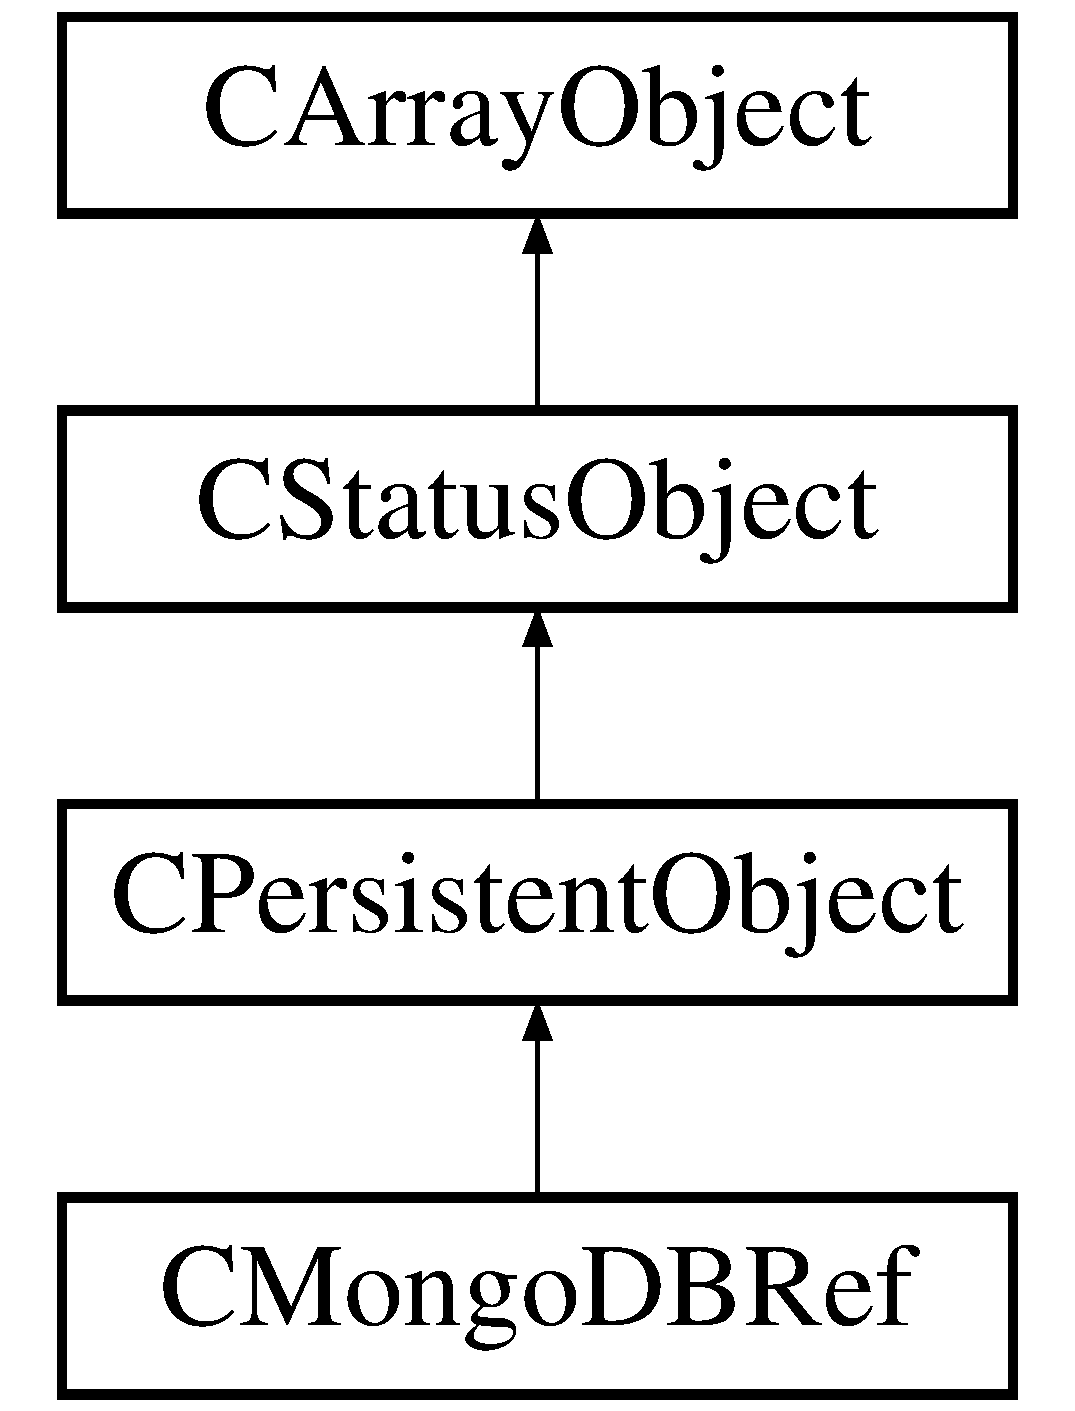
\includegraphics[height=4.000000cm]{class_c_mongo_d_b_ref}
\end{center}
\end{figure}
\subsection*{Public Member Functions}
\begin{DoxyCompactItemize}
\item 
\hyperlink{class_c_mongo_d_b_ref_a13de8db465efc2ac47c38cfc36bce4b9}{\-\_\-\-\_\-construct} (\$the\-Reference=N\-U\-L\-L, \$the\-Container=N\-U\-L\-L)
\item 
\hyperlink{class_c_mongo_d_b_ref_aa7696f05d8742a465b254c8822e69c09}{Resolve} (\$the\-Container)
\item 
\hyperlink{class_c_mongo_d_b_ref_a439141cc81915d0e585f1501813cff01}{Database} (\$the\-Value=N\-U\-L\-L, \$get\-Old=F\-A\-L\-S\-E)
\item 
\hyperlink{class_c_mongo_d_b_ref_ac7ce5aab506229ad1ebdd907e5978ef9}{Collection} (\$the\-Value=N\-U\-L\-L, \$get\-Old=F\-A\-L\-S\-E)
\item 
\hyperlink{class_c_mongo_d_b_ref_addd509a376ff9f56f318345027f4b807}{Identifier} (\$the\-Value=N\-U\-L\-L, \$get\-Old=F\-A\-L\-S\-E)
\item 
\hyperlink{class_c_mongo_d_b_ref_a8c1c4b44c33fc393ba75c9749921c509}{Class\-Name} (\$the\-Value=N\-U\-L\-L, \$get\-Old=F\-A\-L\-S\-E)
\end{DoxyCompactItemize}


\subsection{Constructor \& Destructor Documentation}
\hypertarget{class_c_mongo_d_b_ref_a13de8db465efc2ac47c38cfc36bce4b9}{\index{C\-Mongo\-D\-B\-Ref@{C\-Mongo\-D\-B\-Ref}!\-\_\-\-\_\-construct@{\-\_\-\-\_\-construct}}
\index{\-\_\-\-\_\-construct@{\-\_\-\-\_\-construct}!CMongoDBRef@{C\-Mongo\-D\-B\-Ref}}
\subsubsection[{\-\_\-\-\_\-construct}]{\setlength{\rightskip}{0pt plus 5cm}{\bf C\-Mongo\-D\-B\-Ref\-::\-\_\-\-\_\-construct} (
\begin{DoxyParamCaption}
\item[{\$}]{the\-Reference = {\ttfamily NULL}, }
\item[{\$}]{the\-Container = {\ttfamily NULL}}
\end{DoxyParamCaption}
)}}\label{class_c_mongo_d_b_ref_a13de8db465efc2ac47c38cfc36bce4b9}
Instantiate class.

The constructor will instantiate an object reference in three ways\-:


\begin{DoxyItemize}
\item {\itshape Empty reference\/}\-: Both parameters are omitted or both are {\itshape N\-U\-L\-L\/}. In this case you will have to build the reference by yourself. 
\item {\itshape Object reference\/}\-: The first parameter is provided, the second is not. In this case we assume the first parameter is already an object reference. 
\item {\itshape Object\/}\-: Both parameters are provided, in this case we assume the first parameter is the object to be referenced and the second parameter is the collection from which it was taken; in this case we also record the object \hyperlink{}{class} in the reference. 
\end{DoxyItemize}

In the presence of both parameters, the provided collection takes the precedence over the referenced collection (and database).

When providing either a reference or an object, the class \hyperlink{}{reference} will be set only if the provided reference or object has it.

The parameters to this method are\-:


\begin{DoxyItemize}
\item {\bfseries \$the\-Reference}\-: Either a reference or an object. 
\item {\bfseries \$the\-Container}\-: The collection in which the referenced object resides. 
\end{DoxyItemize}


\begin{DoxyParams}[1]{Parameters}
mixed & {\em \$the\-Reference} & Object, or object reference. \\
\hline
mixed & {\em \$the\-Container} & Object container.\\
\hline
\end{DoxyParams}
public 

Reimplemented from \hyperlink{class_c_persistent_object_a10d0ce97598da33eaf305eb43e418255}{C\-Persistent\-Object}.



\subsection{Member Function Documentation}
\hypertarget{class_c_mongo_d_b_ref_a8c1c4b44c33fc393ba75c9749921c509}{\index{C\-Mongo\-D\-B\-Ref@{C\-Mongo\-D\-B\-Ref}!Class\-Name@{Class\-Name}}
\index{Class\-Name@{Class\-Name}!CMongoDBRef@{C\-Mongo\-D\-B\-Ref}}
\subsubsection[{Class\-Name}]{\setlength{\rightskip}{0pt plus 5cm}{\bf C\-Mongo\-D\-B\-Ref\-::\-Class\-Name} (
\begin{DoxyParamCaption}
\item[{\$}]{the\-Value = {\ttfamily NULL}, }
\item[{\$}]{get\-Old = {\ttfamily FALSE}}
\end{DoxyParamCaption}
)}}\label{class_c_mongo_d_b_ref_a8c1c4b44c33fc393ba75c9749921c509}
Manage referenced object class.

This method can be used to manage the referenced object's \hyperlink{}{class}, it uses the standard accessor \hyperlink{class_c_array_object_a931cb8b30569b811a18adc0161eb3603}{method} to manage the \hyperlink{}{offset}\-:


\begin{DoxyItemize}
\item {\bfseries \$the\-Value}\-: The value or operation\-: 
\begin{DoxyItemize}
\item {\itshape N\-U\-L\-L\/}\-: Return the current value. 
\item {\itshape F\-A\-L\-S\-E\/}\-: Delete the value. 
\item {\itshape other\/}\-: Set value. 
\end{DoxyItemize}
\item {\bfseries \$get\-Old}\-: Determines what the method will return\-: 
\begin{DoxyItemize}
\item {\itshape T\-R\-U\-E\/}\-: Return the value {\itshape before\/} it was eventually modified. 
\item {\itshape F\-A\-L\-S\-E\/}\-: Return the value {\itshape after\/} it was eventually modified. 
\end{DoxyItemize}
\end{DoxyItemize}


\begin{DoxyParams}[1]{Parameters}
N\-U\-L\-L | F\-A\-L\-S\-E | string & {\em \$the\-Value} & User e-\/mail or operation. \\
\hline
boolean & {\em \$get\-Old} & T\-R\-U\-E get old value.\\
\hline
\end{DoxyParams}
public \begin{DoxyReturn}{Returns}
string 
\end{DoxyReturn}
\hypertarget{class_c_mongo_d_b_ref_ac7ce5aab506229ad1ebdd907e5978ef9}{\index{C\-Mongo\-D\-B\-Ref@{C\-Mongo\-D\-B\-Ref}!Collection@{Collection}}
\index{Collection@{Collection}!CMongoDBRef@{C\-Mongo\-D\-B\-Ref}}
\subsubsection[{Collection}]{\setlength{\rightskip}{0pt plus 5cm}{\bf C\-Mongo\-D\-B\-Ref\-::\-Collection} (
\begin{DoxyParamCaption}
\item[{\$}]{the\-Value = {\ttfamily NULL}, }
\item[{\$}]{get\-Old = {\ttfamily FALSE}}
\end{DoxyParamCaption}
)}}\label{class_c_mongo_d_b_ref_ac7ce5aab506229ad1ebdd907e5978ef9}
Manage collection.

This method can be used to manage the database \hyperlink{}{collection}, it uses the standard accessor \hyperlink{class_c_array_object_a931cb8b30569b811a18adc0161eb3603}{method} to manage the \hyperlink{}{offset}\-:


\begin{DoxyItemize}
\item {\bfseries \$the\-Value}\-: The value or operation\-: 
\begin{DoxyItemize}
\item {\itshape N\-U\-L\-L\/}\-: Return the current value. 
\item {\itshape F\-A\-L\-S\-E\/}\-: Delete the value. 
\item {\itshape other\/}\-: Set value. 
\end{DoxyItemize}
\item {\bfseries \$get\-Old}\-: Determines what the method will return\-: 
\begin{DoxyItemize}
\item {\itshape T\-R\-U\-E\/}\-: Return the value {\itshape before\/} it was eventually modified. 
\item {\itshape F\-A\-L\-S\-E\/}\-: Return the value {\itshape after\/} it was eventually modified. 
\end{DoxyItemize}
\end{DoxyItemize}


\begin{DoxyParams}[1]{Parameters}
N\-U\-L\-L | F\-A\-L\-S\-E | string & {\em \$the\-Value} & User code or operation. \\
\hline
boolean & {\em \$get\-Old} & T\-R\-U\-E get old value.\\
\hline
\end{DoxyParams}
public \begin{DoxyReturn}{Returns}
string 
\end{DoxyReturn}
\hypertarget{class_c_mongo_d_b_ref_a439141cc81915d0e585f1501813cff01}{\index{C\-Mongo\-D\-B\-Ref@{C\-Mongo\-D\-B\-Ref}!Database@{Database}}
\index{Database@{Database}!CMongoDBRef@{C\-Mongo\-D\-B\-Ref}}
\subsubsection[{Database}]{\setlength{\rightskip}{0pt plus 5cm}{\bf C\-Mongo\-D\-B\-Ref\-::\-Database} (
\begin{DoxyParamCaption}
\item[{\$}]{the\-Value = {\ttfamily NULL}, }
\item[{\$}]{get\-Old = {\ttfamily FALSE}}
\end{DoxyParamCaption}
)}}\label{class_c_mongo_d_b_ref_a439141cc81915d0e585f1501813cff01}
Manage database.

This method can be used to manage the reference \hyperlink{}{database}, it uses the standard accessor \hyperlink{class_c_array_object_a931cb8b30569b811a18adc0161eb3603}{method} to manage the \hyperlink{}{offset}\-:


\begin{DoxyItemize}
\item {\bfseries \$the\-Value}\-: The value or operation\-: 
\begin{DoxyItemize}
\item {\itshape N\-U\-L\-L\/}\-: Return the current value. 
\item {\itshape F\-A\-L\-S\-E\/}\-: Delete the value. 
\item {\itshape other\/}\-: Set value. 
\end{DoxyItemize}
\item {\bfseries \$get\-Old}\-: Determines what the method will return\-: 
\begin{DoxyItemize}
\item {\itshape T\-R\-U\-E\/}\-: Return the value {\itshape before\/} it was eventually modified. 
\item {\itshape F\-A\-L\-S\-E\/}\-: Return the value {\itshape after\/} it was eventually modified. 
\end{DoxyItemize}
\end{DoxyItemize}


\begin{DoxyParams}[1]{Parameters}
N\-U\-L\-L | F\-A\-L\-S\-E | string & {\em \$the\-Value} & User code or operation. \\
\hline
boolean & {\em \$get\-Old} & T\-R\-U\-E get old value.\\
\hline
\end{DoxyParams}
public \begin{DoxyReturn}{Returns}
string 
\end{DoxyReturn}
\hypertarget{class_c_mongo_d_b_ref_addd509a376ff9f56f318345027f4b807}{\index{C\-Mongo\-D\-B\-Ref@{C\-Mongo\-D\-B\-Ref}!Identifier@{Identifier}}
\index{Identifier@{Identifier}!CMongoDBRef@{C\-Mongo\-D\-B\-Ref}}
\subsubsection[{Identifier}]{\setlength{\rightskip}{0pt plus 5cm}{\bf C\-Mongo\-D\-B\-Ref\-::\-Identifier} (
\begin{DoxyParamCaption}
\item[{\$}]{the\-Value = {\ttfamily NULL}, }
\item[{\$}]{get\-Old = {\ttfamily FALSE}}
\end{DoxyParamCaption}
)}}\label{class_c_mongo_d_b_ref_addd509a376ff9f56f318345027f4b807}
Manage identifier.

This method can be used to manage the collection \hyperlink{}{identifier}, it uses the standard accessor \hyperlink{class_c_array_object_a931cb8b30569b811a18adc0161eb3603}{method} to manage the \hyperlink{}{offset}\-:


\begin{DoxyItemize}
\item {\bfseries \$the\-Value}\-: The value or operation\-: 
\begin{DoxyItemize}
\item {\itshape N\-U\-L\-L\/}\-: Return the current value. 
\item {\itshape F\-A\-L\-S\-E\/}\-: Delete the value. 
\item {\itshape other\/}\-: Set value. 
\end{DoxyItemize}
\item {\bfseries \$get\-Old}\-: Determines what the method will return\-: 
\begin{DoxyItemize}
\item {\itshape T\-R\-U\-E\/}\-: Return the value {\itshape before\/} it was eventually modified. 
\item {\itshape F\-A\-L\-S\-E\/}\-: Return the value {\itshape after\/} it was eventually modified. 
\end{DoxyItemize}
\end{DoxyItemize}


\begin{DoxyParams}[1]{Parameters}
N\-U\-L\-L | F\-A\-L\-S\-E | string & {\em \$the\-Value} & User code or operation. \\
\hline
boolean & {\em \$get\-Old} & T\-R\-U\-E get old value.\\
\hline
\end{DoxyParams}
public \begin{DoxyReturn}{Returns}
string 
\end{DoxyReturn}
\hypertarget{class_c_mongo_d_b_ref_aa7696f05d8742a465b254c8822e69c09}{\index{C\-Mongo\-D\-B\-Ref@{C\-Mongo\-D\-B\-Ref}!Resolve@{Resolve}}
\index{Resolve@{Resolve}!CMongoDBRef@{C\-Mongo\-D\-B\-Ref}}
\subsubsection[{Resolve}]{\setlength{\rightskip}{0pt plus 5cm}{\bf C\-Mongo\-D\-B\-Ref\-::\-Resolve} (
\begin{DoxyParamCaption}
\item[{\$}]{the\-Container}
\end{DoxyParamCaption}
)}}\label{class_c_mongo_d_b_ref_aa7696f05d8742a465b254c8822e69c09}
Resolve the object.

This method should return the referenced object, it accepts a single parameter which should refer to the data store in which the referenced object is saved, in this case either a Mongo\-Collection or a Mongo\-D\-B.


\begin{DoxyParams}[1]{Parameters}
mixed & {\em \$the\-Container} & Data store.\\
\hline
\end{DoxyParams}
public \begin{DoxyReturn}{Returns}
mixed 
\end{DoxyReturn}


The documentation for this class was generated from the following file\-:\begin{DoxyCompactItemize}
\item 
/\-Library/\-Web\-Server/\-Library/wrapper/classes/C\-Mongo\-D\-B\-Ref.\-php\end{DoxyCompactItemize}

\hypertarget{class_c_mongo_query}{\section{C\-Mongo\-Query Class Reference}
\label{class_c_mongo_query}\index{C\-Mongo\-Query@{C\-Mongo\-Query}}
}
Inheritance diagram for C\-Mongo\-Query\-:\begin{figure}[H]
\begin{center}
\leavevmode
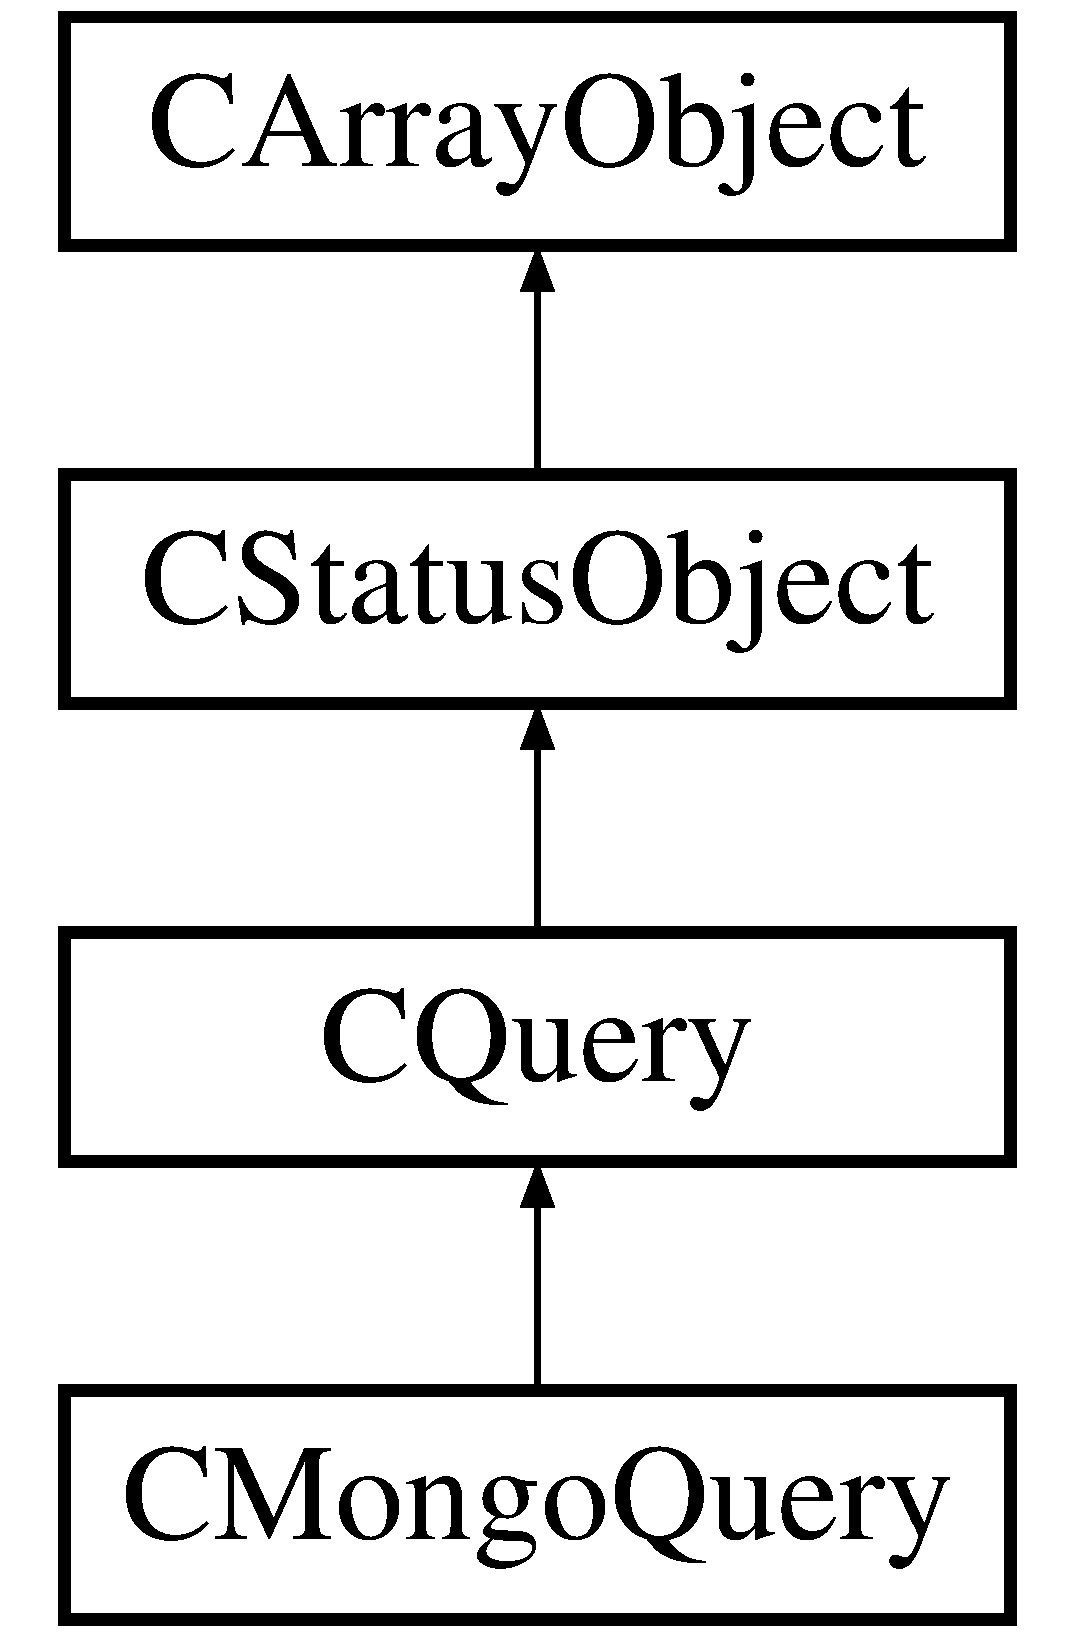
\includegraphics[height=4.000000cm]{class_c_mongo_query}
\end{center}
\end{figure}
\subsection*{Public Member Functions}
\begin{DoxyCompactItemize}
\item 
\hyperlink{class_c_mongo_query_aa25b073480c02f12b91bf262071fa884}{Export} (\$the\-Container)
\end{DoxyCompactItemize}
\subsection*{Protected Member Functions}
\begin{DoxyCompactItemize}
\item 
\hyperlink{class_c_mongo_query_a651af70656cb9894ef1885a711a0c141}{\-\_\-\-Validate\-Condition} (\$the\-Condition, \$the\-Statements, \$the\-Level)
\item 
\hyperlink{class_c_mongo_query_a8cda9306ac308f5c33456e77de004ebb}{\-\_\-\-Convert\-Condition} (\&\$the\-Query, \$the\-Container, \$the\-Condition, \$the\-Statements)
\item 
\hyperlink{class_c_mongo_query_a1f381db3f898f4c9cd333ffd2e3e989b}{\-\_\-\-Convert\-Statement} (\&\$the\-Query, \$the\-Container, \$the\-Condition, \$the\-Statement)
\item 
\hyperlink{class_c_mongo_query_a32fd372e1c39add42d078441eda3f1c3}{\-\_\-\-Order\-Range} (\$the\-Range, \hyperlink{class_c_mongo_container}{C\-Mongo\-Container} \$the\-Container, \$the\-Type)
\end{DoxyCompactItemize}


\subsection{Member Function Documentation}
\hypertarget{class_c_mongo_query_a8cda9306ac308f5c33456e77de004ebb}{\index{C\-Mongo\-Query@{C\-Mongo\-Query}!\-\_\-\-Convert\-Condition@{\-\_\-\-Convert\-Condition}}
\index{\-\_\-\-Convert\-Condition@{\-\_\-\-Convert\-Condition}!CMongoQuery@{C\-Mongo\-Query}}
\subsubsection[{\-\_\-\-Convert\-Condition}]{\setlength{\rightskip}{0pt plus 5cm}C\-Mongo\-Query\-::\-\_\-\-Convert\-Condition (
\begin{DoxyParamCaption}
\item[{\&}]{\$the\-Query, }
\item[{}]{\$the\-Container, }
\item[{}]{\$the\-Condition, }
\item[{}]{\$the\-Statements}
\end{DoxyParamCaption}
)\hspace{0.3cm}{\ttfamily [protected]}}}\label{class_c_mongo_query_a8cda9306ac308f5c33456e77de004ebb}
Convert condition.

This method will convert the statements of the provided condition to Mongo format.

The parameters to this method are\-:


\begin{DoxyItemize}
\item {\bfseries \&\$the\-Query}\-: Reference to an array that will receive the converted condition. 
\item {\bfseries \$the\-Container}\-: Data container, must be derived from \hyperlink{class_c_mongo_container}{C\-Mongo\-Container}. 
\item {\bfseries \$the\-Condition}\-: Boolean condition code. 
\item {\bfseries \$the\-Statements}\-: List of condition statements. 
\end{DoxyItemize}


\begin{DoxyParams}[1]{Parameters}
reference & {\em \&\$the\-Query} & Receives converted query. \\
\hline
\hyperlink{class_c_mongo_container}{C\-Mongo\-Container} & {\em \$the\-Container} & Query container. \\
\hline
string & {\em \$the\-Condition} & Boolean condition. \\
\hline
array & {\em \$the\-Statements} & Statements list.\\
\hline
\end{DoxyParams}
protected \hypertarget{class_c_mongo_query_a1f381db3f898f4c9cd333ffd2e3e989b}{\index{C\-Mongo\-Query@{C\-Mongo\-Query}!\-\_\-\-Convert\-Statement@{\-\_\-\-Convert\-Statement}}
\index{\-\_\-\-Convert\-Statement@{\-\_\-\-Convert\-Statement}!CMongoQuery@{C\-Mongo\-Query}}
\subsubsection[{\-\_\-\-Convert\-Statement}]{\setlength{\rightskip}{0pt plus 5cm}C\-Mongo\-Query\-::\-\_\-\-Convert\-Statement (
\begin{DoxyParamCaption}
\item[{\&}]{\$the\-Query, }
\item[{}]{\$the\-Container, }
\item[{}]{\$the\-Condition, }
\item[{}]{\$the\-Statement}
\end{DoxyParamCaption}
)\hspace{0.3cm}{\ttfamily [protected]}}}\label{class_c_mongo_query_a1f381db3f898f4c9cd333ffd2e3e989b}
Convert statement.

This method will convert the statement to Mongo format.

The parameters to this method are\-:


\begin{DoxyItemize}
\item {\bfseries \&\$the\-Query}\-: Reference to an array that will receive the converted statement. 
\item {\bfseries \$the\-Container}\-: Data container, must be derived from \hyperlink{class_c_mongo_container}{C\-Mongo\-Container} and we assume this check has been done by the \hyperlink{class_c_mongo_query_a8cda9306ac308f5c33456e77de004ebb}{caller}. 
\item {\bfseries \$the\-Condition}\-: Boolean condition code. 
\item {\bfseries \$the\-Statement}\-: Statement. 
\end{DoxyItemize}


\begin{DoxyParams}[1]{Parameters}
reference & {\em \&\$the\-Query} & Receives converted statement. \\
\hline
\hyperlink{class_c_mongo_container}{C\-Mongo\-Container} & {\em \$the\-Container} & Query container. \\
\hline
string & {\em \$the\-Condition} & Boolean condition. \\
\hline
array & {\em \$the\-Statement} & Statement.\\
\hline
\end{DoxyParams}
protected \hypertarget{class_c_mongo_query_a32fd372e1c39add42d078441eda3f1c3}{\index{C\-Mongo\-Query@{C\-Mongo\-Query}!\-\_\-\-Order\-Range@{\-\_\-\-Order\-Range}}
\index{\-\_\-\-Order\-Range@{\-\_\-\-Order\-Range}!CMongoQuery@{C\-Mongo\-Query}}
\subsubsection[{\-\_\-\-Order\-Range}]{\setlength{\rightskip}{0pt plus 5cm}C\-Mongo\-Query\-::\-\_\-\-Order\-Range (
\begin{DoxyParamCaption}
\item[{}]{\$the\-Range, }
\item[{{\bf C\-Mongo\-Container}}]{\$the\-Container, }
\item[{}]{\$the\-Type}
\end{DoxyParamCaption}
)\hspace{0.3cm}{\ttfamily [protected]}}}\label{class_c_mongo_query_a32fd372e1c39add42d078441eda3f1c3}
Order range elements.

This method will order the provided range elements, the method accepts an array of two elements which represent the range bounds and will return an array with the two provided elements sorted.

The method accepts three parameters\-:


\begin{DoxyItemize}
\item {\bfseries \$the\-Range}\-: An array containing two elements representing the range bounds. 
\item {\bfseries \$the\-Container}\-: The \hyperlink{class_c_mongo_container}{container} on which the query will be executed. 
\item {\bfseries \$the\-Type}\-: The data type of the range elements. 
\end{DoxyItemize}

The method expects the range elements to be in \hyperlink{class_c_data_type_a1cae522eec386d293b6087a99e9a8b0b}{serialised} format, these elements will be \hyperlink{class_c_container_a09d585e2a9809221a42d52d7520c9cbf}{converted} by this method which will return them in sorted order.


\begin{DoxyParams}[1]{Parameters}
mixed & {\em \$the\-Range} & Range elements. \\
\hline
C\-Mongo\-Comtainer & {\em \$the\-Container} & Query container. \\
\hline
string & {\em \$the\-Type} & Elements data type.\\
\hline
\end{DoxyParams}
protected \begin{DoxyReturn}{Returns}
array 
\end{DoxyReturn}
\hypertarget{class_c_mongo_query_a651af70656cb9894ef1885a711a0c141}{\index{C\-Mongo\-Query@{C\-Mongo\-Query}!\-\_\-\-Validate\-Condition@{\-\_\-\-Validate\-Condition}}
\index{\-\_\-\-Validate\-Condition@{\-\_\-\-Validate\-Condition}!CMongoQuery@{C\-Mongo\-Query}}
\subsubsection[{\-\_\-\-Validate\-Condition}]{\setlength{\rightskip}{0pt plus 5cm}C\-Mongo\-Query\-::\-\_\-\-Validate\-Condition (
\begin{DoxyParamCaption}
\item[{}]{\$the\-Condition, }
\item[{}]{\$the\-Statements, }
\item[{}]{\$the\-Level}
\end{DoxyParamCaption}
)\hspace{0.3cm}{\ttfamily [protected]}}}\label{class_c_mongo_query_a651af70656cb9894ef1885a711a0c141}
Validate condition.

This method expects a condition as its argument, it will check if it is a valid condition, then it will \hyperlink{class_c_query_afe96707c9ed84ee197dae56c9f05f2a4}{validate} all condition statements.

In this class we handle queries to Mongo databases, so the depth of the query conditions cannot go beyond 2 levels.

We overload this method to prevent nesting O\-R conditions.


\begin{DoxyParams}[1]{Parameters}
string & {\em \$the\-Condition} & Boolean condition. \\
\hline
array & {\em \$the\-Statements} & Statements list. \\
\hline
integer & {\em \$the\-Level} & \mbox{[}P\-R\-I\-V\-A\-T\-E\mbox{]} condition level.\\
\hline
\end{DoxyParams}
protected 

Reimplemented from \hyperlink{class_c_query_a5fbde46df4bb30cb252647f0e47cbbde}{C\-Query}.

\hypertarget{class_c_mongo_query_aa25b073480c02f12b91bf262071fa884}{\index{C\-Mongo\-Query@{C\-Mongo\-Query}!Export@{Export}}
\index{Export@{Export}!CMongoQuery@{C\-Mongo\-Query}}
\subsubsection[{Export}]{\setlength{\rightskip}{0pt plus 5cm}C\-Mongo\-Query\-::\-Export (
\begin{DoxyParamCaption}
\item[{}]{\$the\-Container}
\end{DoxyParamCaption}
)}}\label{class_c_mongo_query_aa25b073480c02f12b91bf262071fa884}
Export query.

The method will return an array suitable to be provided as a Mongo\-D\-B query, the method requires a container that will take care of converting query arguments to native data types, this container must be an instance of \hyperlink{class_c_mongo_container}{C\-Mongo\-Container}, or the method will raise an exception.


\begin{DoxyParams}[1]{Parameters}
\hyperlink{class_c_mongo_container}{C\-Mongo\-Container} & {\em \$the\-Container} & Query container.\\
\hline
\end{DoxyParams}
public \begin{DoxyReturn}{Returns}
array
\end{DoxyReturn}

\begin{DoxyExceptions}{Exceptions}
{\em Exception} & \\
\hline
\end{DoxyExceptions}


The documentation for this class was generated from the following file\-:\begin{DoxyCompactItemize}
\item 
/\-Library/\-Web\-Server/\-Library/wrapper/classes/C\-Mongo\-Query.\-php\end{DoxyCompactItemize}

\hypertarget{class_c_object}{\section{C\-Object Class Reference}
\label{class_c_object}\index{C\-Object@{C\-Object}}
}
Inheritance diagram for C\-Object\-:\begin{figure}[H]
\begin{center}
\leavevmode
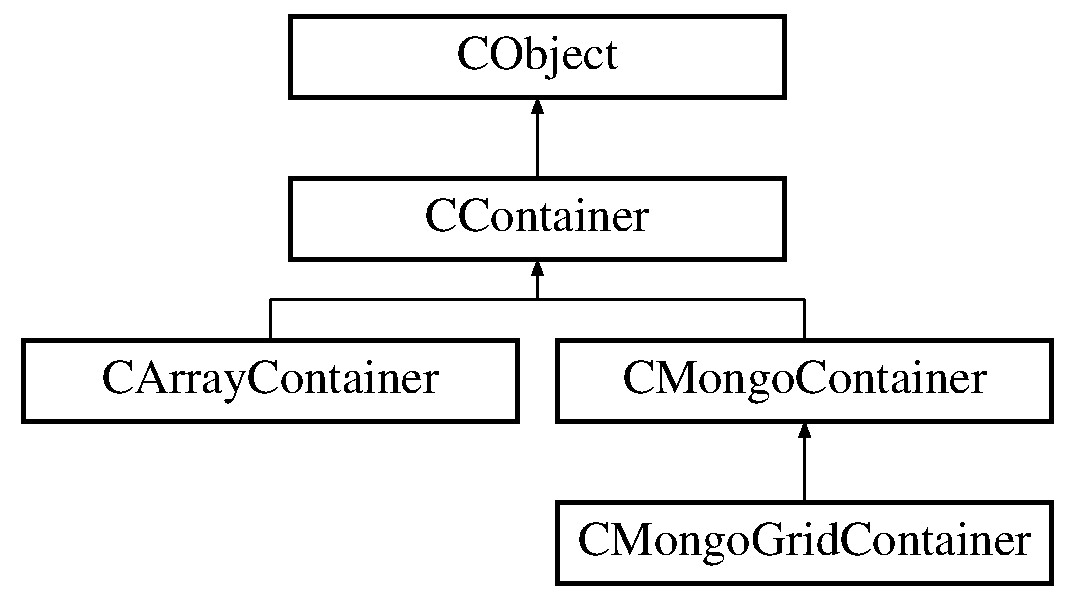
\includegraphics[height=4.000000cm]{class_c_object}
\end{center}
\end{figure}
\subsection*{Static Public Member Functions}
\begin{DoxyCompactItemize}
\item 
static \hyperlink{class_c_object_a660f66b5be21d0cd1156463bcf75e575}{Json\-Encode} (\$the\-Data)
\item 
static \hyperlink{class_c_object_a06eb0f5acf83d67bda8f7946cade841e}{Json\-Decode} (\$the\-Data)
\item 
static \hyperlink{class_c_object_a3c28f63ed5bf37b96c15008f8c825628}{String\-Normalise} (\$the\-String, \$the\-Modifiers=k\-F\-L\-A\-G\-\_\-\-D\-E\-F\-A\-U\-L\-T)
\item 
static \hyperlink{class_c_object_a0255e495d3d0485b50988e496b0249c6}{Duration\-String} (\$the\-Time)
\item 
static \hyperlink{class_c_object_a9b8dccdadcf4fea58f915bd9b228e23e}{Manage\-Member} (\&\$the\-Member, \$the\-Value=N\-U\-L\-L, \$get\-Old=F\-A\-L\-S\-E)
\end{DoxyCompactItemize}


\subsection{Member Function Documentation}
\hypertarget{class_c_object_a0255e495d3d0485b50988e496b0249c6}{\index{C\-Object@{C\-Object}!Duration\-String@{Duration\-String}}
\index{Duration\-String@{Duration\-String}!CObject@{C\-Object}}
\subsubsection[{Duration\-String}]{\setlength{\rightskip}{0pt plus 5cm}static C\-Object\-::\-Duration\-String (
\begin{DoxyParamCaption}
\item[{}]{\$the\-Time}
\end{DoxyParamCaption}
)\hspace{0.3cm}{\ttfamily [static]}}}\label{class_c_object_a0255e495d3d0485b50988e496b0249c6}
Return a formatted duration.

This function will return a formatted duration string in H\-:\-M\-M\-:\-S\-S\-:mmmmm format, where {\itshape H} stands for hours, {\itshape M} stands for minutes, {\itshape S} stands for seconds and {\itshape m} stands for milliseconds, from the value of {\itshape microtime( T\-R\-U\-E )}.

{\itshape Note\-: The provided value should be a difference between two timestamps taken with microtime( true ).}


\begin{DoxyParams}[1]{Parameters}
float & {\em \$the\-Time} & Microtime difference.\\
\hline
\end{DoxyParams}
\begin{DoxyReturn}{Returns}
string 
\end{DoxyReturn}
\hypertarget{class_c_object_a06eb0f5acf83d67bda8f7946cade841e}{\index{C\-Object@{C\-Object}!Json\-Decode@{Json\-Decode}}
\index{Json\-Decode@{Json\-Decode}!CObject@{C\-Object}}
\subsubsection[{Json\-Decode}]{\setlength{\rightskip}{0pt plus 5cm}static C\-Object\-::\-Json\-Decode (
\begin{DoxyParamCaption}
\item[{}]{\$the\-Data}
\end{DoxyParamCaption}
)\hspace{0.3cm}{\ttfamily [static]}}}\label{class_c_object_a06eb0f5acf83d67bda8f7946cade841e}
Return J\-S\-O\-N decoded data.

This method will return an array representation of the provided J\-S\-O\-N string.


\begin{DoxyParams}[1]{Parameters}
string & {\em \$the\-Data} & Input data.\\
\hline
\end{DoxyParams}
\begin{DoxyReturn}{Returns}
array 
\end{DoxyReturn}
\hypertarget{class_c_object_a660f66b5be21d0cd1156463bcf75e575}{\index{C\-Object@{C\-Object}!Json\-Encode@{Json\-Encode}}
\index{Json\-Encode@{Json\-Encode}!CObject@{C\-Object}}
\subsubsection[{Json\-Encode}]{\setlength{\rightskip}{0pt plus 5cm}static C\-Object\-::\-Json\-Encode (
\begin{DoxyParamCaption}
\item[{}]{\$the\-Data}
\end{DoxyParamCaption}
)\hspace{0.3cm}{\ttfamily [static]}}}\label{class_c_object_a660f66b5be21d0cd1156463bcf75e575}
Return J\-S\-O\-N encoded data.

This method will return the provided array or object into a J\-S\-O\-N encoded string.


\begin{DoxyParams}[1]{Parameters}
mixed & {\em \$the\-Data} & Input data.\\
\hline
\end{DoxyParams}
\begin{DoxyReturn}{Returns}
string 
\end{DoxyReturn}
\hypertarget{class_c_object_a9b8dccdadcf4fea58f915bd9b228e23e}{\index{C\-Object@{C\-Object}!Manage\-Member@{Manage\-Member}}
\index{Manage\-Member@{Manage\-Member}!CObject@{C\-Object}}
\subsubsection[{Manage\-Member}]{\setlength{\rightskip}{0pt plus 5cm}static C\-Object\-::\-Manage\-Member (
\begin{DoxyParamCaption}
\item[{\&}]{\$the\-Member, }
\item[{}]{\$the\-Value = {\ttfamily NULL}, }
\item[{}]{\$get\-Old = {\ttfamily FALSE}}
\end{DoxyParamCaption}
)\hspace{0.3cm}{\ttfamily [static]}}}\label{class_c_object_a9b8dccdadcf4fea58f915bd9b228e23e}
Manage a member.

This library implements a standard interface for managing object properties using methods, this method implements this interface\-:


\begin{DoxyItemize}
\item {\bfseries \$the\-Member}\-: The member to manage, it is a reference to the element being managed. 
\item {\bfseries \$the\-Value}\-: The value or operation\-: 
\begin{DoxyItemize}
\item {\itshape N\-U\-L\-L}\-: Return the member's current value. 
\item {\itshape F\-A\-L\-S\-E}\-: Reset the member, {\itshape N\-U\-L\-L} by default. 
\item {\itshape other}\-: Any other type represents the member's new value. 
\end{DoxyItemize}
\item {\bfseries \$get\-Old}\-: Determines what the method will return\-: 
\begin{DoxyItemize}
\item {\itshape T\-R\-U\-E}\-: Return the value of the member {\itshape before} it was eventually modified. 
\item {\itshape F\-A\-L\-S\-E}\-: Return the value of the member {\itshape after} it was eventually modified. 
\end{DoxyItemize}
\end{DoxyItemize}


\begin{DoxyParams}[1]{Parameters}
string & {\em \&\$the\-Member} & Offset. \\
\hline
mixed & {\em \$the\-Value} & Value or operation. \\
\hline
boolean & {\em \$get\-Old} & T\-R\-U\-E get old value.\\
\hline
\end{DoxyParams}
\begin{DoxyReturn}{Returns}
mixed 
\end{DoxyReturn}
\hypertarget{class_c_object_a3c28f63ed5bf37b96c15008f8c825628}{\index{C\-Object@{C\-Object}!String\-Normalise@{String\-Normalise}}
\index{String\-Normalise@{String\-Normalise}!CObject@{C\-Object}}
\subsubsection[{String\-Normalise}]{\setlength{\rightskip}{0pt plus 5cm}static C\-Object\-::\-String\-Normalise (
\begin{DoxyParamCaption}
\item[{}]{\$the\-String, }
\item[{}]{\$the\-Modifiers = {\ttfamily kFLAG\-\_\-DEFAULT}}
\end{DoxyParamCaption}
)\hspace{0.3cm}{\ttfamily [static]}}}\label{class_c_object_a3c28f63ed5bf37b96c15008f8c825628}
Normalise string.

This method can be used to format a string, the provided modifiers bitfield determines what manipulations are applied\-:


\begin{DoxyItemize}
\item {\bfseries \hyperlink{}{k\-F\-L\-A\-G\-\_\-\-M\-O\-D\-I\-F\-I\-E\-R\-\_\-\-U\-T\-F8}}\-: Convert the string to the {\itshape U\-T\-F8} character set. 
\item {\bfseries \hyperlink{}{k\-F\-L\-A\-G\-\_\-\-M\-O\-D\-I\-F\-I\-E\-R\-\_\-\-L\-T\-R\-I\-M}}\-: Apply left trimming to the string. 
\item {\bfseries \hyperlink{}{k\-F\-L\-A\-G\-\_\-\-M\-O\-D\-I\-F\-I\-E\-R\-\_\-\-R\-T\-R\-I\-M}}\-: Apply right trimming to the string. 
\item {\bfseries \hyperlink{}{k\-F\-L\-A\-G\-\_\-\-M\-O\-D\-I\-F\-I\-E\-R\-\_\-\-T\-R\-I\-M}}\-: Apply both left and right trimming to the string. 
\item {\bfseries \hyperlink{}{k\-F\-L\-A\-G\-\_\-\-M\-O\-D\-I\-F\-I\-E\-R\-\_\-\-N\-U\-L\-L}}\-: If this flag is set and the resulting string is empty, the method will return {\itshape N\-U\-L\-L}. 
\begin{DoxyItemize}
\item {\bfseries \hyperlink{}{k\-F\-L\-A\-G\-\_\-\-M\-O\-D\-I\-F\-I\-E\-R\-\_\-\-N\-U\-L\-L\-S\-T\-R}}\-: If this flag is set and the resulting string is empty, the method will return the '{\itshape N\-U\-L\-L}' string; this option implies that the \hyperlink{}{k\-F\-L\-A\-G\-\_\-\-M\-O\-D\-I\-F\-I\-E\-R\-\_\-\-N\-U\-L\-L} is also set. 
\end{DoxyItemize}
\item {\bfseries \hyperlink{}{k\-F\-L\-A\-G\-\_\-\-M\-O\-D\-I\-F\-I\-E\-R\-\_\-\-N\-O\-C\-A\-S\-E}}\-: Set the string to lowercase, this is the default way to generate a case insensitive string. 
\item {\bfseries \hyperlink{}{k\-F\-L\-A\-G\-\_\-\-M\-O\-D\-I\-F\-I\-E\-R\-\_\-\-U\-R\-L}}\-: U\-R\-L-\/encode the string; note that this option and \hyperlink{}{k\-F\-L\-A\-G\-\_\-\-M\-O\-D\-I\-F\-I\-E\-R\-\_\-\-H\-T\-M\-L} are mutually exclusive. 
\item {\bfseries \hyperlink{}{k\-F\-L\-A\-G\-\_\-\-M\-O\-D\-I\-F\-I\-E\-R\-\_\-\-H\-T\-M\-L}}\-: H\-T\-M\-L-\/encode the string; note that this option and \hyperlink{}{k\-F\-L\-A\-G\-\_\-\-M\-O\-D\-I\-F\-I\-E\-R\-\_\-\-U\-R\-L} are mutually exclusive. 
\item {\bfseries \hyperlink{}{k\-F\-L\-A\-G\-\_\-\-M\-O\-D\-I\-F\-I\-E\-R\-\_\-\-H\-E\-X}}\-: Convert the string to hexadecimal; note that this option and \hyperlink{}{hashing} are mutually exclusive. 
\begin{DoxyItemize}
\item {\bfseries \hyperlink{}{k\-F\-L\-A\-G\-\_\-\-M\-O\-D\-I\-F\-I\-E\-R\-\_\-\-H\-E\-X\-E\-X\-P}}\-: Convert the string to a hexadecimal expression; note that this option implies \hyperlink{}{k\-F\-L\-A\-G\-\_\-\-M\-O\-D\-I\-F\-I\-E\-R\-\_\-\-H\-E\-X}, and this option and \hyperlink{}{hashing} are mutually exclusive. 
\end{DoxyItemize}
\item {\bfseries \hyperlink{}{k\-F\-L\-A\-G\-\_\-\-M\-O\-D\-I\-F\-I\-E\-R\-\_\-\-H\-A\-S\-H}}\-: If this bit is set the resulting string will be hashed using the {\itshape md5} algorithm resulting in a 32 character hexadecimal string; this option is mutually exclusive with the \hyperlink{}{k\-F\-L\-A\-G\-\_\-\-M\-O\-D\-I\-F\-I\-E\-R\-\_\-\-M\-A\-S\-K\-\_\-\-H\-E\-X} option. 
\begin{DoxyItemize}
\item {\bfseries \hyperlink{}{k\-F\-L\-A\-G\-\_\-\-M\-O\-D\-I\-F\-I\-E\-R\-\_\-\-H\-A\-S\-H\-\_\-\-B\-I\-N}}\-: If this bit is set, the resulting value should be a 16 character binary string; if the bit is {\itshape O\-F\-F}, the resulting value should be a 32 character hexadecimal string. 
\end{DoxyItemize}
\end{DoxyItemize}

The order in which these modifications are applied are as stated.


\begin{DoxyParams}[1]{Parameters}
string & {\em \$the\-String} & String to normalise. \\
\hline
bitfield & {\em \$the\-Modifiers} & Modifiers bitfield.\\
\hline
\end{DoxyParams}
\begin{DoxyReturn}{Returns}
mixed
\end{DoxyReturn}
\begin{DoxySeeAlso}{See Also}
k\-F\-L\-A\-G\-\_\-\-D\-E\-F\-A\-U\-L\-T, k\-F\-L\-A\-G\-\_\-\-M\-O\-D\-I\-F\-I\-E\-R\-\_\-\-M\-A\-S\-K 

k\-F\-L\-A\-G\-\_\-\-M\-O\-D\-I\-F\-I\-E\-R\-\_\-\-U\-T\-F8 

k\-F\-L\-A\-G\-\_\-\-M\-O\-D\-I\-F\-I\-E\-R\-\_\-\-L\-T\-R\-I\-M, k\-F\-L\-A\-G\-\_\-\-M\-O\-D\-I\-F\-I\-E\-R\-\_\-\-R\-T\-R\-I\-M, k\-F\-L\-A\-G\-\_\-\-M\-O\-D\-I\-F\-I\-E\-R\-\_\-\-T\-R\-I\-M 

k\-F\-L\-A\-G\-\_\-\-M\-O\-D\-I\-F\-I\-E\-R\-\_\-\-N\-U\-L\-L, k\-F\-L\-A\-G\-\_\-\-M\-O\-D\-I\-F\-I\-E\-R\-\_\-\-N\-U\-L\-L\-S\-T\-R 

k\-F\-L\-A\-G\-\_\-\-M\-O\-D\-I\-F\-I\-E\-R\-\_\-\-N\-O\-C\-A\-S\-E, k\-F\-L\-A\-G\-\_\-\-M\-O\-D\-I\-F\-I\-E\-R\-\_\-\-U\-R\-L, k\-F\-L\-A\-G\-\_\-\-M\-O\-D\-I\-F\-I\-E\-R\-\_\-\-H\-T\-M\-L 

k\-F\-L\-A\-G\-\_\-\-M\-O\-D\-I\-F\-I\-E\-R\-\_\-\-H\-E\-X, k\-F\-L\-A\-G\-\_\-\-M\-O\-D\-I\-F\-I\-E\-R\-\_\-\-H\-E\-X\-E\-X\-P 

k\-F\-L\-A\-G\-\_\-\-M\-O\-D\-I\-F\-I\-E\-R\-\_\-\-H\-A\-S\-H, k\-F\-L\-A\-G\-\_\-\-M\-O\-D\-I\-F\-I\-E\-R\-\_\-\-H\-A\-S\-H\-\_\-\-B\-I\-N 
\end{DoxySeeAlso}


The documentation for this class was generated from the following file\-:\begin{DoxyCompactItemize}
\item 
/\-Library/\-Web\-Server/\-Library/wrapper/classes/C\-Object.\-php\end{DoxyCompactItemize}

\hypertarget{class_c_persistent_object}{\section{C\-Persistent\-Object Class Reference}
\label{class_c_persistent_object}\index{C\-Persistent\-Object@{C\-Persistent\-Object}}
}
Inheritance diagram for C\-Persistent\-Object\-:\begin{figure}[H]
\begin{center}
\leavevmode
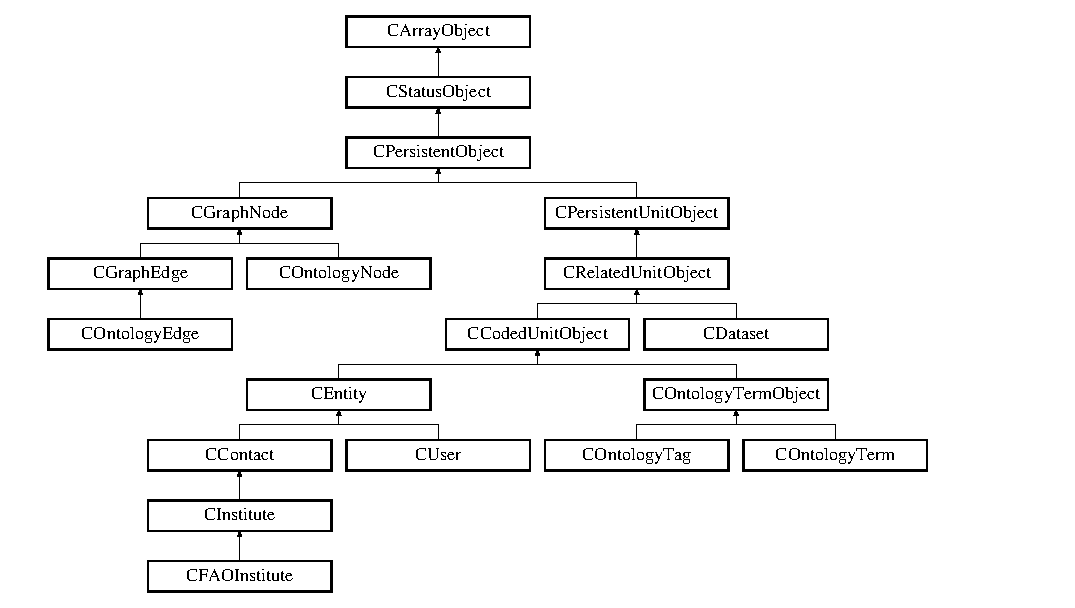
\includegraphics[height=9.655172cm]{class_c_persistent_object}
\end{center}
\end{figure}
\subsection*{Public Member Functions}
\begin{DoxyCompactItemize}
\item 
\hyperlink{class_c_persistent_object_a0f0729cfaef48bd1c98c0711c061a7d3}{\-\_\-\-\_\-construct} (\$the\-Container=N\-U\-L\-L, \$the\-Identifier=N\-U\-L\-L, \$the\-Modifiers=k\-F\-L\-A\-G\-\_\-\-D\-E\-F\-A\-U\-L\-T)
\item 
\hyperlink{class_c_persistent_object_a88b1f2b11d3d60e0b3d33d8b0649b68a}{Commit} (\$the\-Container=N\-U\-L\-L, \$the\-Identifier=N\-U\-L\-L, \$the\-Modifiers=k\-F\-L\-A\-G\-\_\-\-P\-E\-R\-S\-I\-S\-T\-\_\-\-R\-E\-P\-L\-A\-C\-E)
\item 
\hyperlink{class_c_persistent_object_a37c897b534e88477a06ec60b89d84450}{Uncommit} ()
\end{DoxyCompactItemize}
\subsection*{Protected Member Functions}
\begin{DoxyCompactItemize}
\item 
\hyperlink{class_c_persistent_object_a6520a7bcecf3f39fd61ec6d08f736e77}{\-\_\-\-Is\-Committed} (\$the\-State=N\-U\-L\-L)
\item 
\hyperlink{class_c_persistent_object_aa8dc7db66e2af3d28c2035161a2aabf9}{\-\_\-\-Is\-Encoded} (\$the\-State=N\-U\-L\-L)
\item 
\hyperlink{class_c_persistent_object_a584005d1ec0d7e7327dc6d267a9ec50c}{\-\_\-\-Create} (\&\$the\-Content)
\item 
\hyperlink{class_c_persistent_object_ad5376e5aeda7a58e5b27fae6c03b4ef9}{\-\_\-\-Commit} (\&\$the\-Container, \&\$the\-Identifier, \&\$the\-Modifiers)
\item 
\hyperlink{class_c_persistent_object_ada4dfe5bdb0309dee9df94f6e96dc3cb}{\-\_\-\-Load} (\&\$the\-Container, \&\$the\-Identifier, \&\$the\-Modifiers)
\item 
\hyperlink{class_c_persistent_object_a2e5dd4f8a92c0ada964ade712c9579b0}{\-\_\-\-Prepare\-Create} (\&\$the\-Container, \&\$the\-Identifier, \&\$the\-Modifiers)
\item 
\hyperlink{class_c_persistent_object_a5a664513b015919da582c6f0230fab75}{\-\_\-\-Prepare\-Load} (\&\$the\-Container, \&\$the\-Identifier, \&\$the\-Modifiers)
\item 
\hyperlink{class_c_persistent_object_a9d98503112f78729b13995a850b174a8}{\-\_\-\-Prepare\-Commit} (\&\$the\-Container, \&\$the\-Identifier, \&\$the\-Modifiers)
\item 
\hyperlink{class_c_persistent_object_a9029ba173e65e2ec14eeb8bc7c2024c6}{\-\_\-\-Finish\-Create} (\&\$the\-Container)
\item 
\hyperlink{class_c_persistent_object_a35ffbe4e875e03a84985493bbce75457}{\-\_\-\-Finish\-Load} (\&\$the\-Container, \&\$the\-Identifier, \&\$the\-Modifiers)
\item 
\hyperlink{class_c_persistent_object_a535a2f078b777a144d31117de054ccf7}{\-\_\-\-Finish\-Commit} (\&\$the\-Container, \&\$the\-Identifier, \&\$the\-Modifiers)
\item 
\hyperlink{class_c_persistent_object_a948ba9d69729dfe20564aecdb9d4fae7}{\-\_\-\-Set\-Tags} (\$the\-Offset=k\-T\-A\-G\-\_\-\-T\-A\-G\-S)
\item 
\hyperlink{class_c_persistent_object_a7a9363dc8aba31cf00e382172ba327bd}{\-\_\-\-Get\-Tags} ()
\end{DoxyCompactItemize}
\subsection*{Additional Inherited Members}


\subsection{Constructor \& Destructor Documentation}
\hypertarget{class_c_persistent_object_a0f0729cfaef48bd1c98c0711c061a7d3}{\index{C\-Persistent\-Object@{C\-Persistent\-Object}!\-\_\-\-\_\-construct@{\-\_\-\-\_\-construct}}
\index{\-\_\-\-\_\-construct@{\-\_\-\-\_\-construct}!CPersistentObject@{C\-Persistent\-Object}}
\subsubsection[{\-\_\-\-\_\-construct}]{\setlength{\rightskip}{0pt plus 5cm}C\-Persistent\-Object\-::\-\_\-\-\_\-construct (
\begin{DoxyParamCaption}
\item[{}]{\$the\-Container = {\ttfamily NULL}, }
\item[{}]{\$the\-Identifier = {\ttfamily NULL}, }
\item[{}]{\$the\-Modifiers = {\ttfamily kFLAG\-\_\-DEFAULT}}
\end{DoxyParamCaption}
)}}\label{class_c_persistent_object_a0f0729cfaef48bd1c98c0711c061a7d3}
Instantiate class.

The constructor can be used to instantiate an empty object, instantiate an object from some content, or load an object from a container.

The parameters to this method are\-:


\begin{DoxyItemize}
\item {\bfseries \$the\-Container}\-: This parameter represents either the {\itshape contents} of the object, if the next parameter is missing, or the {\itshape \hyperlink{class_c_container}{container}} in which the object resides. If missing, we assume we want to create an empty object. 
\begin{DoxyItemize}
\item {\itshape N\-U\-L\-L}\-: In this case it is assumed you want to instantiate an empty object and the next parameter will be ignored. 
\item {\itshape Array} or {\itshape Array\-Object}\-: In this case we assume the parameter represents either the object contents, if the next parameter is {\itshape N\-U\-L\-L}, or the \hyperlink{class_c_container}{container} in which the object is \hyperlink{class_c_persistent_object_a88b1f2b11d3d60e0b3d33d8b0649b68a}{stored}, in which case we interpret the next parameter to be the object's identifier. 
\item {\itshape Other}\-: Any other type will raise an \hyperlink{}{exception}, or it should be handled by derived classes. 
\end{DoxyItemize}
\item {\bfseries \$the\-Identifier}\-: This parameter represents the key or query that will be used to locate the object in the container provided in the first parameter. 
\begin{DoxyItemize}
\item {\itshape N\-U\-L\-L}\-: This indicates that the first parameter represents the object {\itshape contents}. 
\item {\itshape other}\-: Any other type is considered as a key or query used to locate the object in the container provided in the first parameter. 
\end{DoxyItemize}
\item {\bfseries \$the\-Modifiers}\-: This bitfield parameter can be used to provide a series of options to the object. The available options can be consulted in \hyperlink{}{this} file. Most of these options are managed automatically and should not be provided explicitly. This class handles one option that has the following meaning\-: 
\begin{DoxyItemize}
\item {\itshape \hyperlink{}{k\-F\-L\-A\-G\-\_\-\-S\-T\-A\-T\-E\-\_\-\-E\-N\-C\-O\-D\-E\-D}}\-: If the option is on, the object will be passed through a \hyperlink{class_c_container_aa339d3c4c9b011713176a89fe9c7783d}{conversion} process that will convert all \hyperlink{class_c_data_type}{standard} data types into native container custom data types \hyperlink{class_c_container_a0dc47e54abc533cedf1c2c0f915d96b2}{before} \hyperlink{class_c_persistent_object_a88b1f2b11d3d60e0b3d33d8b0649b68a}{committing} the object; the opposite \hyperlink{class_c_data_type_a608d6fc184bce537ce83669f729d6008}{conversion} process will take place \hyperlink{class_c_container_ab53bd683f0e28b2203897cf03f9d1c76}{after} \hyperlink{class_c_persistent_object_a0f0729cfaef48bd1c98c0711c061a7d3}{loading} the object from a container. It is a good idea to keep this flag O\-N, because the converted object will be compatible with any \hyperlink{class_c_container}{container} and it will make data transfers from one database to the other easy. This process is automatic and transparent. 
\end{DoxyItemize}
\end{DoxyItemize}

Depending on the results of this method we set the \hyperlink{class_c_persistent_object_a6520a7bcecf3f39fd61ec6d08f736e77}{committed} status \hyperlink{}{flag} as follows\-:


\begin{DoxyItemize}
\item {\itshape Empty object}\-: By omitting the first parameter we indicate that we want to start from scratch, the object will not have its \hyperlink{class_c_persistent_object_a6520a7bcecf3f39fd61ec6d08f736e77}{committed} \hyperlink{}{flag} set. 
\item {\itshape Filled object}\-: In this case we provide in the {\itshape \$the\-Container} parameter the object's {\itshape contents}. In this case we do not consider the object as persistent, so the object will not have its \hyperlink{class_c_persistent_object_a6520a7bcecf3f39fd61ec6d08f736e77}{committed} \hyperlink{}{flag} set. 
\item {\itshape Selected object}\-: In this case we search the {\itshape \$the\-Container} with the provided {\itshape \$the\-Identifier} as a key or query, and if\-: 
\begin{DoxyItemize}
\item {\itshape Found}\-: We set the \hyperlink{class_c_persistent_object_a6520a7bcecf3f39fd61ec6d08f736e77}{committed} \hyperlink{}{flag} on. 
\item {\itshape Not found}\-: We instantiate an empty object and ignore the \hyperlink{class_c_persistent_object_a6520a7bcecf3f39fd61ec6d08f736e77}{committed} \hyperlink{}{flag}. 
\end{DoxyItemize}
\end{DoxyItemize}

The \hyperlink{class_c_status_object_a8429102e4f52f7558649b64f4e673a69}{inited} status \hyperlink{}{flag} is not set by default, this will prevent the object from being \hyperlink{class_c_persistent_object_a88b1f2b11d3d60e0b3d33d8b0649b68a}{stored} and it is the responsibility of derived concrete instances to manage this status.

This method takes advantage of a protected interface which should be overloaded by derived classes instead of overloading this method\-:


\begin{DoxyItemize}
\item {\itshape Retrieve object}\-: If the second parameter was provided, it implies that the object is to be retrieved from the first parameter which represents the \hyperlink{class_c_container}{container} in which the object contents are stored. 
\begin{DoxyItemize}
\item {\itshape \hyperlink{class_c_persistent_object_a5a664513b015919da582c6f0230fab75}{\-\_\-\-Prepare\-Load}()}\-: This method should check and normalise the container and identifier. In this class we ensure that the container is derived from \hyperlink{class_c_container}{C\-Container}. 
\item {\itshape \hyperlink{class_c_persistent_object_ada4dfe5bdb0309dee9df94f6e96dc3cb}{\-\_\-\-Load}()}\-: This method will delegate the \hyperlink{class_c_container}{container} the responsibility of locating and retrieving the object using the provided identifier. 
\end{DoxyItemize}
\item {\itshape \hyperlink{class_c_persistent_object_a584005d1ec0d7e7327dc6d267a9ec50c}{\-\_\-\-Create}()}\-: This method should instantiate the object from the contents returned by \hyperlink{class_c_persistent_object_ada4dfe5bdb0309dee9df94f6e96dc3cb}{\-\_\-\-Load} or by the data provided in the first parameter in the case the second parameter was omitted. 
\end{DoxyItemize}

Derived classes should overload the above interface rather than overloading this method and should do so only if necessary, because this workflow should be sufficient for persisting objects.


\begin{DoxyParams}[1]{Parameters}
mixed & {\em \$the\-Container} & Persistent container. \\
\hline
mixed & {\em \$the\-Identifier} & Object identifier. \\
\hline
bitfield & {\em \$the\-Modifiers} & Create modifiers.\\
\hline
\end{DoxyParams}
public

\hyperlink{class_c_persistent_object_a5a664513b015919da582c6f0230fab75}{\-\_\-\-Prepare\-Load()}  \hyperlink{class_c_persistent_object_ada4dfe5bdb0309dee9df94f6e96dc3cb}{\-\_\-\-Load()}  \hyperlink{class_c_persistent_object_a584005d1ec0d7e7327dc6d267a9ec50c}{\-\_\-\-Create()}  \hyperlink{class_c_persistent_object_a6520a7bcecf3f39fd61ec6d08f736e77}{\-\_\-\-Is\-Committed()}  \hyperlink{class_c_persistent_object_a35ffbe4e875e03a84985493bbce75457}{\-\_\-\-Finish\-Load()}  \hyperlink{class_c_persistent_object_a9029ba173e65e2ec14eeb8bc7c2024c6}{\-\_\-\-Finish\-Create()} 

Reimplemented in \hyperlink{class_c_user_af83ffccb40893a43d90eafe396cbdec1}{C\-User}, \hyperlink{class_c_institute_a468ba723fabd5a67bea5016d1531b147}{C\-Institute}, \hyperlink{class_c_ontology_term_a33679101b2a63044f0084918a8df123e}{C\-Ontology\-Term}, \hyperlink{class_c_coded_unit_object_a314fc62af62314f5ac5acca2ac809900}{C\-Coded\-Unit\-Object}, and \hyperlink{class_c_ontology_term_object_af1fb502088538ad7372719c20f73bc5c}{C\-Ontology\-Term\-Object}.



\subsection{Member Function Documentation}
\hypertarget{class_c_persistent_object_ad5376e5aeda7a58e5b27fae6c03b4ef9}{\index{C\-Persistent\-Object@{C\-Persistent\-Object}!\-\_\-\-Commit@{\-\_\-\-Commit}}
\index{\-\_\-\-Commit@{\-\_\-\-Commit}!CPersistentObject@{C\-Persistent\-Object}}
\subsubsection[{\-\_\-\-Commit}]{\setlength{\rightskip}{0pt plus 5cm}C\-Persistent\-Object\-::\-\_\-\-Commit (
\begin{DoxyParamCaption}
\item[{\&}]{\$the\-Container, }
\item[{\&}]{\$the\-Identifier, }
\item[{\&}]{\$the\-Modifiers}
\end{DoxyParamCaption}
)\hspace{0.3cm}{\ttfamily [protected]}}}\label{class_c_persistent_object_ad5376e5aeda7a58e5b27fae6c03b4ef9}
Store object in container.

The duty of this method is to store the current object in the container provided in the first parameter with as key the value provided in the second parameter with options provided in the third parameter, please refer to \hyperlink{class_c_persistent_object_a88b1f2b11d3d60e0b3d33d8b0649b68a}{this} documentation for a reference of these parameters. Note that in this method all three parameters are passed by reference.

This class supports \hyperlink{class_c_container}{C\-Container} derived instances and will delegate the operation to the container. Note that by default we call the container's \hyperlink{class_c_container_a4847dc676d1f7704e75f8981e927508a}{commit} method with the \hyperlink{}{k\-F\-L\-A\-G\-\_\-\-P\-E\-R\-S\-I\-S\-T\-\_\-\-R\-E\-P\-L\-A\-C\-E} option, which will \hyperlink{}{insert} the object if new or \hyperlink{}{replace} the eventual existing object.

The method expects all parameters to have been previously \hyperlink{class_c_persistent_object_a9d98503112f78729b13995a850b174a8}{checked}, its main duty is to perform the actual storage. In derived classes you should intercept custom containers, or call the parent method.

{\itshape Note\-: the duty of this method is to store only the array part of the object, properties should be ignored.}


\begin{DoxyParams}[1]{Parameters}
reference & {\em \&\$the\-Container} & Object container. \\
\hline
reference & {\em \&\$the\-Identifier} & Object identifier. \\
\hline
reference & {\em \&\$the\-Modifiers} & Commit modifiers.\\
\hline
\end{DoxyParams}
protected \begin{DoxyReturn}{Returns}
mixed 
\end{DoxyReturn}


Reimplemented in \hyperlink{class_c_ontology_node_a590c869a08d167ba35d987e450106a2d}{C\-Ontology\-Node}, \hyperlink{class_c_graph_node_a7af17771eaba24551f8c9a465f391c23}{C\-Graph\-Node}, \hyperlink{class_c_persistent_unit_object_ae8726af138967ed9b4b2edbfa2a188a3}{C\-Persistent\-Unit\-Object}, \hyperlink{class_c_ontology_edge_a76e551f21dcac3c0bc228c67226bec08}{C\-Ontology\-Edge}, and \hyperlink{class_c_graph_edge_a73dd2ced3103285f8ad4ea212c0e918e}{C\-Graph\-Edge}.

\hypertarget{class_c_persistent_object_a584005d1ec0d7e7327dc6d267a9ec50c}{\index{C\-Persistent\-Object@{C\-Persistent\-Object}!\-\_\-\-Create@{\-\_\-\-Create}}
\index{\-\_\-\-Create@{\-\_\-\-Create}!CPersistentObject@{C\-Persistent\-Object}}
\subsubsection[{\-\_\-\-Create}]{\setlength{\rightskip}{0pt plus 5cm}C\-Persistent\-Object\-::\-\_\-\-Create (
\begin{DoxyParamCaption}
\item[{\&}]{\$the\-Content}
\end{DoxyParamCaption}
)\hspace{0.3cm}{\ttfamily [protected]}}}\label{class_c_persistent_object_a584005d1ec0d7e7327dc6d267a9ec50c}
Create object.

The duty of this method is to instantiate an object with the provided data.

The method expects one parameter which is passed by reference\-:


\begin{DoxyItemize}
\item {\bfseries \&\$the\-Content}\-: This parameter represents the object contents\-: 
\begin{DoxyItemize}
\item {\itshape N\-U\-L\-L}\-: The method will instantiate an empty object. 
\item {\itshape array} or an {\itshape Array\-Object}\-: The method will instantiate the object with the contents of the provided parameter. 
\item {\itshape other}\-: By default any other type will raise an exception, in derived classes you can overload this method to handle custom types. 
\end{DoxyItemize}
\end{DoxyItemize}

The method returns a boolean where {\itshape T\-R\-U\-E} indicates that the object was instantiated with data, and {\itshape F\-A\-L\-S\-E} indicating that the object is empty. This will be used by the \hyperlink{class_c_persistent_object_a0f0729cfaef48bd1c98c0711c061a7d3}{caller} to set the object \hyperlink{class_c_persistent_object_a6520a7bcecf3f39fd61ec6d08f736e77}{committed} status \hyperlink{}{flag}.

The parameter is provided as a reference.


\begin{DoxyParams}[1]{Parameters}
reference & {\em \&\$the\-Content} & Object data content.\\
\hline
\end{DoxyParams}
protected \begin{DoxyReturn}{Returns}
boolean
\end{DoxyReturn}

\begin{DoxyExceptions}{Exceptions}
{\em \{@link} & \hyperlink{class_c_exception}{C\-Exception} \hyperlink{class_c_exception}{C\-Exception}\}\\
\hline
\end{DoxyExceptions}
\begin{DoxySeeAlso}{See also}
k\-E\-R\-R\-O\-R\-\_\-\-U\-N\-S\-U\-P\-P\-O\-R\-T\-E\-D 
\end{DoxySeeAlso}


Reimplemented in \hyperlink{class_c_graph_node_a90e49bf5e95ccf3c8644196696154268}{C\-Graph\-Node}.

\hypertarget{class_c_persistent_object_a535a2f078b777a144d31117de054ccf7}{\index{C\-Persistent\-Object@{C\-Persistent\-Object}!\-\_\-\-Finish\-Commit@{\-\_\-\-Finish\-Commit}}
\index{\-\_\-\-Finish\-Commit@{\-\_\-\-Finish\-Commit}!CPersistentObject@{C\-Persistent\-Object}}
\subsubsection[{\-\_\-\-Finish\-Commit}]{\setlength{\rightskip}{0pt plus 5cm}C\-Persistent\-Object\-::\-\_\-\-Finish\-Commit (
\begin{DoxyParamCaption}
\item[{\&}]{\$the\-Container, }
\item[{\&}]{\$the\-Identifier, }
\item[{\&}]{\$the\-Modifiers}
\end{DoxyParamCaption}
)\hspace{0.3cm}{\ttfamily [protected]}}}\label{class_c_persistent_object_a535a2f078b777a144d31117de054ccf7}
Normalise after a \hyperlink{class_c_persistent_object_ad5376e5aeda7a58e5b27fae6c03b4ef9}{commit}.

This method will be called after the \hyperlink{class_c_persistent_object_ad5376e5aeda7a58e5b27fae6c03b4ef9}{store} operation, its duty is to clean up or restore the object after the operation please refer to \hyperlink{class_c_persistent_object_a88b1f2b11d3d60e0b3d33d8b0649b68a}{this} documentation for a reference of these parameters. Note that in this method all three parameters are passed by reference.

In this class we set the \hyperlink{class_c_persistent_object_a6520a7bcecf3f39fd61ec6d08f736e77}{commit} \hyperlink{}{flag} and reset the \hyperlink{class_c_status_object_a19c4ac94dfe26476e780d77b99744d43}{dirty} \hyperlink{}{flag}.


\begin{DoxyParams}[1]{Parameters}
reference & {\em \&\$the\-Container} & Object container. \\
\hline
reference & {\em \&\$the\-Identifier} & Object identifier. \\
\hline
reference & {\em \&\$the\-Modifiers} & Commit modifiers.\\
\hline
\end{DoxyParams}
protected \hypertarget{class_c_persistent_object_a9029ba173e65e2ec14eeb8bc7c2024c6}{\index{C\-Persistent\-Object@{C\-Persistent\-Object}!\-\_\-\-Finish\-Create@{\-\_\-\-Finish\-Create}}
\index{\-\_\-\-Finish\-Create@{\-\_\-\-Finish\-Create}!CPersistentObject@{C\-Persistent\-Object}}
\subsubsection[{\-\_\-\-Finish\-Create}]{\setlength{\rightskip}{0pt plus 5cm}C\-Persistent\-Object\-::\-\_\-\-Finish\-Create (
\begin{DoxyParamCaption}
\item[{\&}]{\$the\-Container}
\end{DoxyParamCaption}
)\hspace{0.3cm}{\ttfamily [protected]}}}\label{class_c_persistent_object_a9029ba173e65e2ec14eeb8bc7c2024c6}
Normalise after a \hyperlink{class_c_persistent_object_a584005d1ec0d7e7327dc6d267a9ec50c}{create}.

This method will be called after the \hyperlink{class_c_persistent_object_a584005d1ec0d7e7327dc6d267a9ec50c}{create} operation, its duty is to initialise an empty object. Both the container and the identifier parameters are passed by reference.

This method will be called if the identifier was not provided to the \hyperlink{class_c_persistent_object_a0f0729cfaef48bd1c98c0711c061a7d3}{constructor}, or if the \hyperlink{class_c_persistent_object_a0f0729cfaef48bd1c98c0711c061a7d3}{constructor} was unable to \hyperlink{class_c_persistent_object_ada4dfe5bdb0309dee9df94f6e96dc3cb}{find} the requested object.

In this class we do nothing.


\begin{DoxyParams}[1]{Parameters}
reference & {\em \&\$the\-Container} & Object container.\\
\hline
\end{DoxyParams}
protected 

Reimplemented in \hyperlink{class_c_ontology_node_a3f116a2f1a1047da5187f21e20d3d405}{C\-Ontology\-Node}, \hyperlink{class_c_graph_node_a8a8df45cff2375d0bcbb15342ae3960b}{C\-Graph\-Node}, \hyperlink{class_c_ontology_edge_a0956d5920484a329c77d878bb6c25784}{C\-Ontology\-Edge}, and \hyperlink{class_c_graph_edge_a42fd83eff1eef079a6005e961fd2d371}{C\-Graph\-Edge}.

\hypertarget{class_c_persistent_object_a35ffbe4e875e03a84985493bbce75457}{\index{C\-Persistent\-Object@{C\-Persistent\-Object}!\-\_\-\-Finish\-Load@{\-\_\-\-Finish\-Load}}
\index{\-\_\-\-Finish\-Load@{\-\_\-\-Finish\-Load}!CPersistentObject@{C\-Persistent\-Object}}
\subsubsection[{\-\_\-\-Finish\-Load}]{\setlength{\rightskip}{0pt plus 5cm}C\-Persistent\-Object\-::\-\_\-\-Finish\-Load (
\begin{DoxyParamCaption}
\item[{\&}]{\$the\-Container, }
\item[{\&}]{\$the\-Identifier, }
\item[{\&}]{\$the\-Modifiers}
\end{DoxyParamCaption}
)\hspace{0.3cm}{\ttfamily [protected]}}}\label{class_c_persistent_object_a35ffbe4e875e03a84985493bbce75457}
Normalise after a \hyperlink{class_c_persistent_object_ada4dfe5bdb0309dee9df94f6e96dc3cb}{load}.

This method will be called after the \hyperlink{class_c_persistent_object_ada4dfe5bdb0309dee9df94f6e96dc3cb}{load} operation, its duty is to clean up or normalise after the operation. Both the container and the identifier parameters are passed by reference.

In this class we do nothing.


\begin{DoxyParams}[1]{Parameters}
reference & {\em \&\$the\-Container} & Object container. \\
\hline
reference & {\em \&\$the\-Identifier} & Object identifier. \\
\hline
reference & {\em \&\$the\-Modifiers} & Create modifiers.\\
\hline
\end{DoxyParams}
protected 

Reimplemented in \hyperlink{class_c_ontology_node_a97c5e875641e3bb3da83d32ed8b26ebc}{C\-Ontology\-Node}, \hyperlink{class_c_graph_node_a23c2beb0fbed1ab67018dd9d78dee8fa}{C\-Graph\-Node}, \hyperlink{class_c_ontology_edge_ac45af3396c797be599c2a1780b7bfa59}{C\-Ontology\-Edge}, and \hyperlink{class_c_graph_edge_a7cbf3dab4745b0924905fce01e383819}{C\-Graph\-Edge}.

\hypertarget{class_c_persistent_object_a7a9363dc8aba31cf00e382172ba327bd}{\index{C\-Persistent\-Object@{C\-Persistent\-Object}!\-\_\-\-Get\-Tags@{\-\_\-\-Get\-Tags}}
\index{\-\_\-\-Get\-Tags@{\-\_\-\-Get\-Tags}!CPersistentObject@{C\-Persistent\-Object}}
\subsubsection[{\-\_\-\-Get\-Tags}]{\setlength{\rightskip}{0pt plus 5cm}C\-Persistent\-Object\-::\-\_\-\-Get\-Tags (
\begin{DoxyParamCaption}
{}
\end{DoxyParamCaption}
)\hspace{0.3cm}{\ttfamily [protected]}}}\label{class_c_persistent_object_a7a9363dc8aba31cf00e382172ba327bd}
Get attribute tags.

The duty of this method is to collect all attribute tags used in the object and return them as an array.

protected \begin{DoxyReturn}{Returns}
array 
\end{DoxyReturn}


Reimplemented in \hyperlink{class_c_persistent_unit_object_ac4df6b15733c79b93493131275a27493}{C\-Persistent\-Unit\-Object}.

\hypertarget{class_c_persistent_object_a6520a7bcecf3f39fd61ec6d08f736e77}{\index{C\-Persistent\-Object@{C\-Persistent\-Object}!\-\_\-\-Is\-Committed@{\-\_\-\-Is\-Committed}}
\index{\-\_\-\-Is\-Committed@{\-\_\-\-Is\-Committed}!CPersistentObject@{C\-Persistent\-Object}}
\subsubsection[{\-\_\-\-Is\-Committed}]{\setlength{\rightskip}{0pt plus 5cm}C\-Persistent\-Object\-::\-\_\-\-Is\-Committed (
\begin{DoxyParamCaption}
\item[{}]{\$the\-State = {\ttfamily NULL}}
\end{DoxyParamCaption}
)\hspace{0.3cm}{\ttfamily [protected]}}}\label{class_c_persistent_object_a6520a7bcecf3f39fd61ec6d08f736e77}
Manage committed status.

This method can be used to get or set the object's committed state.

A committed object is one that has either been loaded from a container or committed to a container. This state indicates that the object is persistent. This state, combined with the \hyperlink{class_c_status_object_a19c4ac94dfe26476e780d77b99744d43}{dirty} status, can determine if an object needs to be committed in a container or not.

The method features a single parameter\-:


\begin{DoxyItemize}
\item {\itshape N\-U\-L\-L}\-: The method will return {\itshape T\-R\-U\-E} if the object is committed, or {\itshape F\-A\-L\-S\-E} if the object is not committed. 
\item {\itshape T\-R\-U\-E}\-: The method will set the object to committed. 
\item {\itshape F\-A\-L\-S\-E}\-: The method will reset the object's committed state. 
\end{DoxyItemize}

In all cases the method will return the state {\itshape after} it was eventually modified.


\begin{DoxyParams}[1]{Parameters}
mixed & {\em \$the\-State} & T\-R\-U\-E, F\-A\-L\-S\-E or N\-U\-L\-L.\\
\hline
\end{DoxyParams}
protected \begin{DoxyReturn}{Returns}
boolean
\end{DoxyReturn}
\hyperlink{class_c_status_object_a3e37d72a6462d93bf7ff567f07f78093}{\-\_\-\-Manage\-Bit\-Field()}

\begin{DoxySeeAlso}{See also}
k\-F\-L\-A\-G\-\_\-\-S\-T\-A\-T\-E\-\_\-\-C\-O\-M\-M\-I\-T\-T\-E\-D 
\end{DoxySeeAlso}
\hypertarget{class_c_persistent_object_aa8dc7db66e2af3d28c2035161a2aabf9}{\index{C\-Persistent\-Object@{C\-Persistent\-Object}!\-\_\-\-Is\-Encoded@{\-\_\-\-Is\-Encoded}}
\index{\-\_\-\-Is\-Encoded@{\-\_\-\-Is\-Encoded}!CPersistentObject@{C\-Persistent\-Object}}
\subsubsection[{\-\_\-\-Is\-Encoded}]{\setlength{\rightskip}{0pt plus 5cm}C\-Persistent\-Object\-::\-\_\-\-Is\-Encoded (
\begin{DoxyParamCaption}
\item[{}]{\$the\-State = {\ttfamily NULL}}
\end{DoxyParamCaption}
)\hspace{0.3cm}{\ttfamily [protected]}}}\label{class_c_persistent_object_aa8dc7db66e2af3d28c2035161a2aabf9}
Manage encoded status.

This method can be used to get or set the object's encoded state.

This flag determines whether custom data types are to be converted to \hyperlink{class_c_data_type}{standard} types when working with the object. This is especially useful when transmitting the object through the network or when managing custom database types.

The conversion to \hyperlink{class_c_data_type}{standard} types is \hyperlink{class_c_data_type_a608d6fc184bce537ce83669f729d6008}{done} when \hyperlink{class_c_persistent_object_a0f0729cfaef48bd1c98c0711c061a7d3}{loading} the object from a \hyperlink{class_c_container}{container} and the opposite is \hyperlink{class_c_container_aa339d3c4c9b011713176a89fe9c7783d}{done} before \hyperlink{class_c_persistent_object_a88b1f2b11d3d60e0b3d33d8b0649b68a}{storing} the object into a \hyperlink{class_c_container}{container}, these operations are performed by the \hyperlink{class_c_container}{container} object that takes care of object persistence.

This \hyperlink{}{k\-F\-L\-A\-G\-\_\-\-S\-T\-A\-T\-E\-\_\-\-E\-N\-C\-O\-D\-E\-D} flag can be provided at \hyperlink{class_c_persistent_object_a0f0729cfaef48bd1c98c0711c061a7d3}{instantiation} or directly to the persistence methods, although it is a better idea to provide it in the \hyperlink{class_c_persistent_object_a0f0729cfaef48bd1c98c0711c061a7d3}{constructor} to have this conversion happen transparently.

The method features a single parameter\-:


\begin{DoxyItemize}
\item {\itshape N\-U\-L\-L}\-: The method will return {\itshape T\-R\-U\-E} if the object is encoded, or {\itshape F\-A\-L\-S\-E} if the object is not encoded. 
\item {\itshape T\-R\-U\-E}\-: The method will set the object to encoded. 
\item {\itshape F\-A\-L\-S\-E}\-: The method will reset the object's encoded state. 
\end{DoxyItemize}

In all cases the method will return the state {\itshape after} it was eventually modified.


\begin{DoxyParams}[1]{Parameters}
mixed & {\em \$the\-State} & T\-R\-U\-E, F\-A\-L\-S\-E or N\-U\-L\-L.\\
\hline
\end{DoxyParams}
protected \begin{DoxyReturn}{Returns}
boolean
\end{DoxyReturn}
\hyperlink{class_c_status_object_a3e37d72a6462d93bf7ff567f07f78093}{\-\_\-\-Manage\-Bit\-Field()}

\begin{DoxySeeAlso}{See also}
k\-F\-L\-A\-G\-\_\-\-S\-T\-A\-T\-E\-\_\-\-E\-N\-C\-O\-D\-E\-D 
\end{DoxySeeAlso}
\hypertarget{class_c_persistent_object_ada4dfe5bdb0309dee9df94f6e96dc3cb}{\index{C\-Persistent\-Object@{C\-Persistent\-Object}!\-\_\-\-Load@{\-\_\-\-Load}}
\index{\-\_\-\-Load@{\-\_\-\-Load}!CPersistentObject@{C\-Persistent\-Object}}
\subsubsection[{\-\_\-\-Load}]{\setlength{\rightskip}{0pt plus 5cm}C\-Persistent\-Object\-::\-\_\-\-Load (
\begin{DoxyParamCaption}
\item[{\&}]{\$the\-Container, }
\item[{\&}]{\$the\-Identifier, }
\item[{\&}]{\$the\-Modifiers}
\end{DoxyParamCaption}
)\hspace{0.3cm}{\ttfamily [protected]}}}\label{class_c_persistent_object_ada4dfe5bdb0309dee9df94f6e96dc3cb}
Find object.

The duty of this method is to locate the object identified by {\itshape \$the\-Identifier} in the container {\itshape \$the\-Container} and return its contents or {\itshape N\-U\-L\-L} if not found.

The method should expect both parameters to have been previously checked\-: in this class, the container must be an {\itshape Array\-Object} representing either the actual container, or a \hyperlink{class_c_container}{C\-Container} derived instance which will take care of locating the object within its managed native container.


\begin{DoxyParams}[1]{Parameters}
reference & {\em \&\$the\-Container} & Object container. \\
\hline
reference & {\em \&\$the\-Identifier} & Object identifier. \\
\hline
reference & {\em \&\$the\-Modifiers} & Create options.\\
\hline
\end{DoxyParams}
protected \begin{DoxyReturn}{Returns}
mixed 
\end{DoxyReturn}


Reimplemented in \hyperlink{class_c_ontology_node_a7a8304ab0e782d621012edddd8e7da3a}{C\-Ontology\-Node}, \hyperlink{class_c_graph_node_a60c57e754245042fe04dad8fb63a5fec}{C\-Graph\-Node}, \hyperlink{class_c_ontology_edge_ae7a4861887c1a73dcdbd0285cdba1d8d}{C\-Ontology\-Edge}, and \hyperlink{class_c_graph_edge_a8c19599c8543c9c1a25b9c2dfba8e223}{C\-Graph\-Edge}.

\hypertarget{class_c_persistent_object_a9d98503112f78729b13995a850b174a8}{\index{C\-Persistent\-Object@{C\-Persistent\-Object}!\-\_\-\-Prepare\-Commit@{\-\_\-\-Prepare\-Commit}}
\index{\-\_\-\-Prepare\-Commit@{\-\_\-\-Prepare\-Commit}!CPersistentObject@{C\-Persistent\-Object}}
\subsubsection[{\-\_\-\-Prepare\-Commit}]{\setlength{\rightskip}{0pt plus 5cm}C\-Persistent\-Object\-::\-\_\-\-Prepare\-Commit (
\begin{DoxyParamCaption}
\item[{\&}]{\$the\-Container, }
\item[{\&}]{\$the\-Identifier, }
\item[{\&}]{\$the\-Modifiers}
\end{DoxyParamCaption}
)\hspace{0.3cm}{\ttfamily [protected]}}}\label{class_c_persistent_object_a9d98503112f78729b13995a850b174a8}
Normalise before a store.

This method will be called before the \hyperlink{class_c_persistent_object_ad5376e5aeda7a58e5b27fae6c03b4ef9}{store} operation, its duty is to prepare the object and check the parameters for the \hyperlink{class_c_persistent_object_ad5376e5aeda7a58e5b27fae6c03b4ef9}{commit} operation, please refer to \hyperlink{class_c_persistent_object_a88b1f2b11d3d60e0b3d33d8b0649b68a}{this} documentation for a reference of these parameters. Note that in this method all three parameters are passed by reference.

By default we perform the following checks\-:


\begin{DoxyItemize}
\item Ensure the container is provided. 
\item Ensure the identifier is provided if \hyperlink{}{updating}. 
\item Ensure the object is \hyperlink{class_c_status_object_a8429102e4f52f7558649b64f4e673a69}{initialised}. 
\end{DoxyItemize}

In derived classes you should handle your custom containers or delegate to the parent method.

In this class we do not check the identifier.

Any errors should raise an exception.


\begin{DoxyParams}[1]{Parameters}
reference & {\em \&\$the\-Container} & Object container. \\
\hline
reference & {\em \&\$the\-Identifier} & Object identifier. \\
\hline
reference & {\em \&\$the\-Modifiers} & Commit modifiers.\\
\hline
\end{DoxyParams}
protected


\begin{DoxyExceptions}{Exceptions}
{\em \{@link} & \hyperlink{class_c_exception}{C\-Exception} \hyperlink{class_c_exception}{C\-Exception}\}\\
\hline
\end{DoxyExceptions}
\hyperlink{class_c_status_object_a8429102e4f52f7558649b64f4e673a69}{\-\_\-\-Is\-Inited()}

\begin{DoxySeeAlso}{See also}
k\-E\-R\-R\-O\-R\-\_\-\-I\-N\-V\-A\-L\-I\-D\-\_\-\-S\-T\-A\-T\-E k\-E\-R\-R\-O\-R\-\_\-\-O\-P\-T\-I\-O\-N\-\_\-\-M\-I\-S\-S\-I\-N\-G k\-E\-R\-R\-O\-R\-\_\-\-U\-N\-S\-U\-P\-P\-O\-R\-T\-E\-D 
\end{DoxySeeAlso}


Reimplemented in \hyperlink{class_c_ontology_node_a460df05b73fd4160e7a652ed3b03dd78}{C\-Ontology\-Node}, \hyperlink{class_c_graph_node_ad55d35f1ac947bae32fe8019daf05112}{C\-Graph\-Node}, \hyperlink{class_c_ontology_edge_a2bea996dff6e836069d75572f9386039}{C\-Ontology\-Edge}, \hyperlink{class_c_persistent_unit_object_aaa69a5dd56c441027197d5cb677972ad}{C\-Persistent\-Unit\-Object}, \hyperlink{class_c_f_a_o_institute_a9917150b0e31b741aa10c9443e880746}{C\-F\-A\-O\-Institute}, \hyperlink{class_c_ontology_term_a5d10f6baf1e484591d1d99b325e22d89}{C\-Ontology\-Term}, \hyperlink{class_c_ontology_term_object_aca3572974abb180f507fc63264a9ba15}{C\-Ontology\-Term\-Object}, \hyperlink{class_c_related_unit_object_a577c73999830641e07440126a3252286}{C\-Related\-Unit\-Object}, \hyperlink{class_c_institute_a096aa38309ae2f88250700d5755a18a6}{C\-Institute}, \hyperlink{class_c_user_aacdc43c5a38cb6b013ee9ce686b186e9}{C\-User}, and \hyperlink{class_c_entity_ac306808f0f8404fa405674cbe14fd441}{C\-Entity}.

\hypertarget{class_c_persistent_object_a2e5dd4f8a92c0ada964ade712c9579b0}{\index{C\-Persistent\-Object@{C\-Persistent\-Object}!\-\_\-\-Prepare\-Create@{\-\_\-\-Prepare\-Create}}
\index{\-\_\-\-Prepare\-Create@{\-\_\-\-Prepare\-Create}!CPersistentObject@{C\-Persistent\-Object}}
\subsubsection[{\-\_\-\-Prepare\-Create}]{\setlength{\rightskip}{0pt plus 5cm}C\-Persistent\-Object\-::\-\_\-\-Prepare\-Create (
\begin{DoxyParamCaption}
\item[{\&}]{\$the\-Container, }
\item[{\&}]{\$the\-Identifier, }
\item[{\&}]{\$the\-Modifiers}
\end{DoxyParamCaption}
)\hspace{0.3cm}{\ttfamily [protected]}}}\label{class_c_persistent_object_a2e5dd4f8a92c0ada964ade712c9579b0}
Normalise parameters of a create.

The duty of this method is to ensure that the parameters provided to a \hyperlink{class_c_persistent_object_a584005d1ec0d7e7327dc6d267a9ec50c}{create} operation are valid.

The method has a chance to work with the container and the identifier before it is set in the object.

In this class we set the \hyperlink{class_c_persistent_object_aa8dc7db66e2af3d28c2035161a2aabf9}{encoded} status \hyperlink{}{flag} if provided among the modifiers of the operation.


\begin{DoxyParams}[1]{Parameters}
reference & {\em \&\$the\-Container} & Object container. \\
\hline
reference & {\em \&\$the\-Identifier} & Object identifier. \\
\hline
reference & {\em \&\$the\-Modifiers} & Create modifiers.\\
\hline
\end{DoxyParams}
protected

\hyperlink{class_c_persistent_object_aa8dc7db66e2af3d28c2035161a2aabf9}{\-\_\-\-Is\-Encoded()}

\begin{DoxySeeAlso}{See also}
k\-F\-L\-A\-G\-\_\-\-S\-T\-A\-T\-E\-\_\-\-E\-N\-C\-O\-D\-E\-D 
\end{DoxySeeAlso}


Reimplemented in \hyperlink{class_c_ontology_node_a8dd4c8bc984a535448618bbbba987a55}{C\-Ontology\-Node}, \hyperlink{class_c_graph_node_a500c59ddfbec7fedf8598ee5d886de67}{C\-Graph\-Node}, \hyperlink{class_c_ontology_edge_a1d09b3ef8e4ef57a072291a7c09f7371}{C\-Ontology\-Edge}, \hyperlink{class_c_ontology_term_object_a7e785a79bf4c20b094450e688e3e73cf}{C\-Ontology\-Term\-Object}, and \hyperlink{class_c_entity_a4fdef5f86472b284c53a876d72ba8b07}{C\-Entity}.

\hypertarget{class_c_persistent_object_a5a664513b015919da582c6f0230fab75}{\index{C\-Persistent\-Object@{C\-Persistent\-Object}!\-\_\-\-Prepare\-Load@{\-\_\-\-Prepare\-Load}}
\index{\-\_\-\-Prepare\-Load@{\-\_\-\-Prepare\-Load}!CPersistentObject@{C\-Persistent\-Object}}
\subsubsection[{\-\_\-\-Prepare\-Load}]{\setlength{\rightskip}{0pt plus 5cm}C\-Persistent\-Object\-::\-\_\-\-Prepare\-Load (
\begin{DoxyParamCaption}
\item[{\&}]{\$the\-Container, }
\item[{\&}]{\$the\-Identifier, }
\item[{\&}]{\$the\-Modifiers}
\end{DoxyParamCaption}
)\hspace{0.3cm}{\ttfamily [protected]}}}\label{class_c_persistent_object_a5a664513b015919da582c6f0230fab75}
Normalise parameters of a find.

The duty of this method is to ensure that the parameters provided to a \hyperlink{class_c_persistent_object_ada4dfe5bdb0309dee9df94f6e96dc3cb}{find} operation are valid.

The method should first check if the provided container is of the correct type, then it should ensure that the identifier is valid.

We know that the identifier cannot be missing, since this method is only called if the identifier was provided. We should check that the provided container is of the correct type. In derived classes you should first handle your custom types, then let the parent method handle other types.

Any errors should raise an exception.

In this class we only support \hyperlink{class_c_container}{C\-Container} containers and the identifier is not expected to be {\itshape N\-U\-L\-L}.


\begin{DoxyParams}[1]{Parameters}
reference & {\em \&\$the\-Container} & Object container. \\
\hline
reference & {\em \&\$the\-Identifier} & Object identifier. \\
\hline
reference & {\em \&\$the\-Modifiers} & Create modifiers.\\
\hline
\end{DoxyParams}
protected


\begin{DoxyExceptions}{Exceptions}
{\em \{@link} & \hyperlink{class_c_exception}{C\-Exception} \hyperlink{class_c_exception}{C\-Exception}\}\\
\hline
\end{DoxyExceptions}
\hyperlink{class_c_persistent_object_aa8dc7db66e2af3d28c2035161a2aabf9}{\-\_\-\-Is\-Encoded()}

\begin{DoxySeeAlso}{See also}
k\-E\-R\-R\-O\-R\-\_\-\-O\-P\-T\-I\-O\-N\-\_\-\-M\-I\-S\-S\-I\-N\-G k\-E\-R\-R\-O\-R\-\_\-\-U\-N\-S\-U\-P\-P\-O\-R\-T\-E\-D 
\end{DoxySeeAlso}


Reimplemented in \hyperlink{class_c_ontology_node_ac8a77d7437a9be4b4aa18626b1a9f95d}{C\-Ontology\-Node}, \hyperlink{class_c_graph_node_af9f27bcc601672903af33f33d62e7ebf}{C\-Graph\-Node}, \hyperlink{class_c_ontology_edge_a6099442ba1dca683e4832d406793b5b9}{C\-Ontology\-Edge}, and \hyperlink{class_c_persistent_unit_object_a5f41b9143a5ae8fb353989c26d4ee301}{C\-Persistent\-Unit\-Object}.

\hypertarget{class_c_persistent_object_a948ba9d69729dfe20564aecdb9d4fae7}{\index{C\-Persistent\-Object@{C\-Persistent\-Object}!\-\_\-\-Set\-Tags@{\-\_\-\-Set\-Tags}}
\index{\-\_\-\-Set\-Tags@{\-\_\-\-Set\-Tags}!CPersistentObject@{C\-Persistent\-Object}}
\subsubsection[{\-\_\-\-Set\-Tags}]{\setlength{\rightskip}{0pt plus 5cm}C\-Persistent\-Object\-::\-\_\-\-Set\-Tags (
\begin{DoxyParamCaption}
\item[{}]{\$the\-Offset = {\ttfamily kTAG\-\_\-TAGS}}
\end{DoxyParamCaption}
)\hspace{0.3cm}{\ttfamily [protected]}}}\label{class_c_persistent_object_a948ba9d69729dfe20564aecdb9d4fae7}
Set attribute tags.

The duty of this method is to collect all attribute tags used in the object and store them as an array at the provided offset.

The method will collect all attributes, overload this method to exclude default attributes.


\begin{DoxyParams}[1]{Parameters}
string & {\em \$the\-Offset} & Offset.\\
\hline
\end{DoxyParams}
protected \hypertarget{class_c_persistent_object_a88b1f2b11d3d60e0b3d33d8b0649b68a}{\index{C\-Persistent\-Object@{C\-Persistent\-Object}!Commit@{Commit}}
\index{Commit@{Commit}!CPersistentObject@{C\-Persistent\-Object}}
\subsubsection[{Commit}]{\setlength{\rightskip}{0pt plus 5cm}C\-Persistent\-Object\-::\-Commit (
\begin{DoxyParamCaption}
\item[{}]{\$the\-Container = {\ttfamily NULL}, }
\item[{}]{\$the\-Identifier = {\ttfamily NULL}, }
\item[{}]{\$the\-Modifiers = {\ttfamily kFLAG\-\_\-PERSIST\-\_\-REPLACE}}
\end{DoxyParamCaption}
)}}\label{class_c_persistent_object_a88b1f2b11d3d60e0b3d33d8b0649b68a}
Commit the object into a container.

This method should be used to commit the object to a container, the method accepts two parameters\-:


\begin{DoxyItemize}
\item {\bfseries \$the\-Container}\-: This parameter represents the {\itshape container} in which the object is to be stored. By default we enforce concrete instances of \hyperlink{class_c_container}{C\-Container}, derived classes may overload the protected interface to initialise this value. 
\item {\bfseries \$the\-Identifier}\-: This parameter represents the value by which the current object will be uniquely identified in the first parameter. By default this value is required, derived classes may overload the protected interface to initialise this value. 
\item {\bfseries \$the\-Modifiers}\-: This parameter represents the commit operation options, by default we assume you want to \hyperlink{}{replace} an object, but you may change this value if you want to perform specific commit operations\-: 
\begin{DoxyItemize}
\item {\itshape \hyperlink{}{k\-F\-L\-A\-G\-\_\-\-P\-E\-R\-S\-I\-S\-T\-\_\-\-I\-N\-S\-E\-R\-T}}\-: The provided object will be inserted in the container, it is assumed that no other element in the container shares the same identifier, in that case the container \hyperlink{class_c_container_a4847dc676d1f7704e75f8981e927508a}{method} must raise an \hyperlink{}{exception}. 
\item {\itshape \hyperlink{}{k\-F\-L\-A\-G\-\_\-\-P\-E\-R\-S\-I\-S\-T\-\_\-\-U\-P\-D\-A\-T\-E}}\-: The provided object will replace the existing object. In this case the method expects the container to have an entry with the same key as the provided identifier, if this is not the case the container \hyperlink{class_c_container_a4847dc676d1f7704e75f8981e927508a}{method} must raise an \hyperlink{}{exception}. With this option it is assumed that the provided object's attributes will replace all the existing object's ones. 
\item {\itshape \hyperlink{}{k\-F\-L\-A\-G\-\_\-\-P\-E\-R\-S\-I\-S\-T\-\_\-\-M\-O\-D\-I\-F\-Y}}\-: The provided object is assumed to contain a subset of an existing object's attributes, these provided attributes will be appended or replace the existing ones. In this case the method expects the container to have an entry with the same key as the provided identifier, if this is not the case the method must raise an \hyperlink{}{exception}. 
\item {\itshape \hyperlink{}{k\-F\-L\-A\-G\-\_\-\-P\-E\-R\-S\-I\-S\-T\-\_\-\-R\-E\-P\-L\-A\-C\-E}}\-: The provided object will be \hyperlink{}{inserted}, if the identifier doesn't match any container elements, or it will \hyperlink{}{replace} the existing object. As with \hyperlink{}{update}, it is assumed that the provided object's attributes will replace all the existing object's ones. 
\item {\itshape \hyperlink{}{k\-F\-L\-A\-G\-\_\-\-P\-E\-R\-S\-I\-S\-T\-\_\-\-D\-E\-L\-E\-T\-E}}\-: This option assumes you want to remove the object from the container, although the container features a specific \hyperlink{class_c_container_aa91ec2f4624a2ebfb74668f274139329}{method} for this purpose, this option may be used to implement a {\itshape deleted state}, rather than actually removing the object from the container. 
\item {\itshape \hyperlink{}{k\-F\-L\-A\-G\-\_\-\-S\-T\-A\-T\-E\-\_\-\-E\-N\-C\-O\-D\-E\-D}}\-: If the option is on, the object will be passed through a \hyperlink{class_c_container_aa339d3c4c9b011713176a89fe9c7783d}{conversion} process that will convert all \hyperlink{class_c_data_type}{standard} data types into native container custom data types \hyperlink{class_c_container_a0dc47e54abc533cedf1c2c0f915d96b2}{before} committing the object. It is a good idea to keep this flag O\-N, because the converted object will be compatible with any \hyperlink{class_c_container}{container} and it will make data transfers from one database to the other easy. This process is automatic and transparent. 
\end{DoxyItemize}
\end{DoxyItemize}

The method will only operate if either the \hyperlink{class_c_persistent_object_a6520a7bcecf3f39fd61ec6d08f736e77}{committed} \hyperlink{}{flag} is {\itshape not set}, or the \hyperlink{class_c_status_object_a19c4ac94dfe26476e780d77b99744d43}{dirty} \hyperlink{}{flag} is {\itshape set}, if none of these two conditions are satisfied, the method will do nothing.

The method will by default {\itshape set} the \hyperlink{class_c_persistent_object_a6520a7bcecf3f39fd61ec6d08f736e77}{committed} \hyperlink{}{flag} and {\itshape reset} the \hyperlink{class_c_status_object_a19c4ac94dfe26476e780d77b99744d43}{dirty} \hyperlink{}{flag} if the operation was successful.

This method should raise an exception if any error occurs.

The method should return the unique identifier of the object or {\itshape N\-U\-L\-L} if the operation was not performed.

In derived classes you should not overload this method, instead, you should overload the protected interface\-:


\begin{DoxyItemize}
\item {\itshape \hyperlink{class_c_persistent_object_a9d98503112f78729b13995a850b174a8}{\-\_\-\-Prepare\-Commit}()}\-: This method can be used to initialise or check the parameters and resources. 
\item {\itshape \hyperlink{class_c_persistent_object_ad5376e5aeda7a58e5b27fae6c03b4ef9}{\-\_\-\-Commit}()}\-: This method will perform the actual commit. 
\item {\itshape \hyperlink{class_c_persistent_object_a535a2f078b777a144d31117de054ccf7}{\-\_\-\-Finish\-Commit}()}\-: This method can be used to perform eventual post-\/flight adjustments. 
\end{DoxyItemize}


\begin{DoxyParams}[1]{Parameters}
mixed & {\em \$the\-Container} & Persistent container. \\
\hline
mixed & {\em \$the\-Identifier} & Object identifier. \\
\hline
bitfield & {\em \$the\-Modifiers} & Commit modifiers.\\
\hline
\end{DoxyParams}
public \begin{DoxyReturn}{Returns}
mixed
\end{DoxyReturn}
\hyperlink{class_c_status_object_a19c4ac94dfe26476e780d77b99744d43}{\-\_\-\-Is\-Dirty()}  \hyperlink{class_c_persistent_object_a6520a7bcecf3f39fd61ec6d08f736e77}{\-\_\-\-Is\-Committed()}  \hyperlink{class_c_persistent_object_a9d98503112f78729b13995a850b174a8}{\-\_\-\-Prepare\-Commit()}  \hyperlink{class_c_persistent_object_ad5376e5aeda7a58e5b27fae6c03b4ef9}{\-\_\-\-Commit()}  \hyperlink{class_c_persistent_object_a535a2f078b777a144d31117de054ccf7}{\-\_\-\-Finish\-Commit()}

\begin{DoxySeeAlso}{See also}
k\-F\-L\-A\-G\-\_\-\-P\-E\-R\-S\-I\-S\-T\-\_\-\-I\-N\-S\-E\-R\-T k\-F\-L\-A\-G\-\_\-\-P\-E\-R\-S\-I\-S\-T\-\_\-\-U\-P\-D\-A\-T\-E k\-F\-L\-A\-G\-\_\-\-P\-E\-R\-S\-I\-S\-T\-\_\-\-M\-O\-D\-I\-F\-Y 

k\-F\-L\-A\-G\-\_\-\-P\-E\-R\-S\-I\-S\-T\-\_\-\-R\-E\-P\-L\-A\-C\-E k\-F\-L\-A\-G\-\_\-\-S\-T\-A\-T\-E\-\_\-\-E\-N\-C\-O\-D\-E\-D 
\end{DoxySeeAlso}
\hypertarget{class_c_persistent_object_a37c897b534e88477a06ec60b89d84450}{\index{C\-Persistent\-Object@{C\-Persistent\-Object}!Uncommit@{Uncommit}}
\index{Uncommit@{Uncommit}!CPersistentObject@{C\-Persistent\-Object}}
\subsubsection[{Uncommit}]{\setlength{\rightskip}{0pt plus 5cm}C\-Persistent\-Object\-::\-Uncommit (
\begin{DoxyParamCaption}
{}
\end{DoxyParamCaption}
)}}\label{class_c_persistent_object_a37c897b534e88477a06ec60b89d84450}
Reset \hyperlink{class_c_persistent_object_a6520a7bcecf3f39fd61ec6d08f736e77}{committed} status.

This method can be used to reset the object's \hyperlink{}{committed} \hyperlink{class_c_persistent_object_a6520a7bcecf3f39fd61ec6d08f736e77}{status}, this may be necessary when copying an object from one container to the other, since the object will be \hyperlink{class_c_persistent_object_a88b1f2b11d3d60e0b3d33d8b0649b68a}{committed} only if the \hyperlink{}{committed} \hyperlink{class_c_persistent_object_a6520a7bcecf3f39fd61ec6d08f736e77}{status} is not set, or if the \hyperlink{}{dirty} \hyperlink{class_c_status_object_a19c4ac94dfe26476e780d77b99744d43}{status} is set.

public

\hyperlink{class_c_persistent_object_a6520a7bcecf3f39fd61ec6d08f736e77}{\-\_\-\-Is\-Committed()} 

The documentation for this class was generated from the following file\-:\begin{DoxyCompactItemize}
\item 
/\-Library/\-Web\-Server/\-Library/wrapper/classes/C\-Persistent\-Object.\-php\end{DoxyCompactItemize}

\hypertarget{class_c_persistent_unit_object}{\section{C\-Persistent\-Unit\-Object Class Reference}
\label{class_c_persistent_unit_object}\index{C\-Persistent\-Unit\-Object@{C\-Persistent\-Unit\-Object}}
}
Inheritance diagram for C\-Persistent\-Unit\-Object\-:\begin{figure}[H]
\begin{center}
\leavevmode
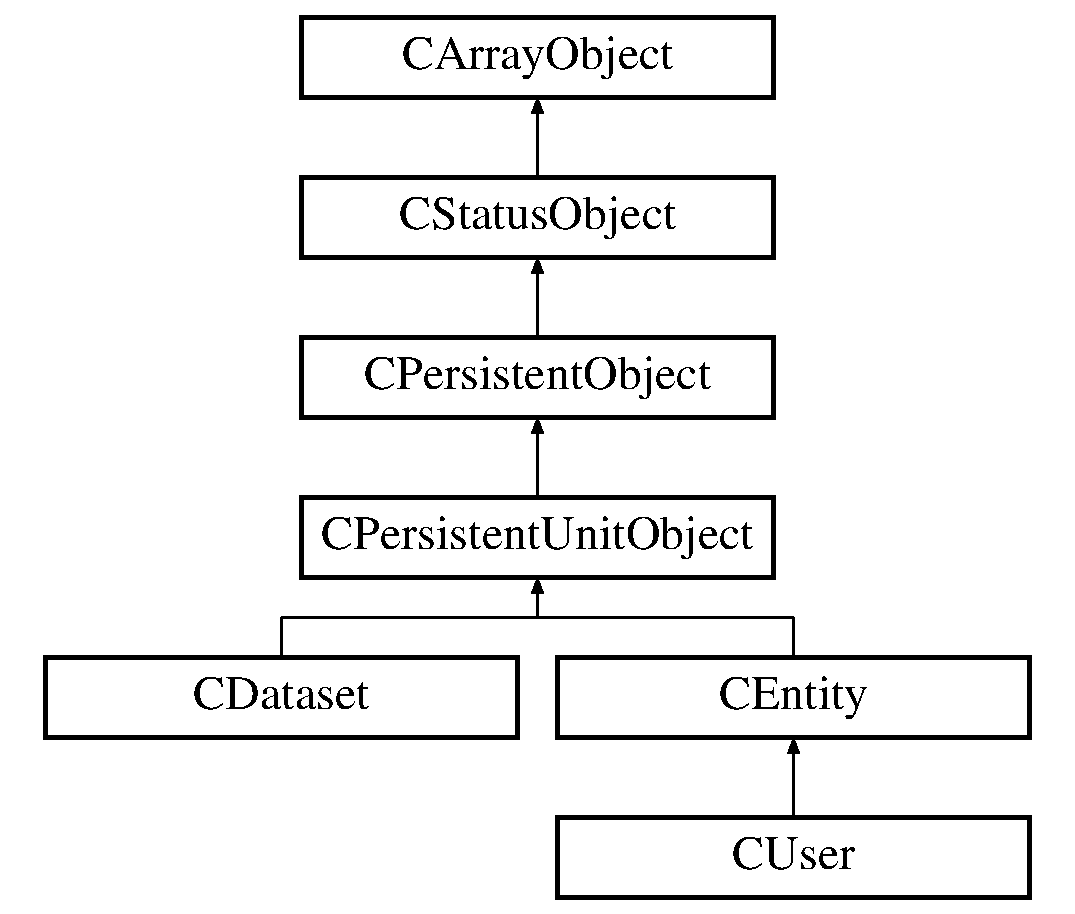
\includegraphics[height=10.000000cm]{class_c_persistent_unit_object}
\end{center}
\end{figure}
\subsection*{Public Member Functions}
\begin{DoxyCompactItemize}
\item 
\hyperlink{class_c_persistent_unit_object_af75b0a5542f5d14a9a2879e5d3864cac}{\-\_\-\-\_\-to\-String} ()
\item 
\hyperlink{class_c_persistent_unit_object_a953695de3bbfc5c3d76d0b9b3a39f6a1}{Persistent} ()
\end{DoxyCompactItemize}
\subsection*{Static Public Member Functions}
\begin{DoxyCompactItemize}
\item 
static \hyperlink{class_c_persistent_unit_object_ab3e33158e9b08a45f3a0b71feb922f50}{New\-Object} (\$the\-Container, \$the\-Identifier, \$the\-Modifiers=k\-F\-L\-A\-G\-\_\-\-D\-E\-F\-A\-U\-L\-T)
\item 
static \hyperlink{class_c_persistent_unit_object_a45700a911c2266de6e562cdd62c3c777}{Reference} (\$the\-Object, \$the\-Modifiers=k\-F\-L\-A\-G\-\_\-\-R\-E\-F\-E\-R\-E\-N\-C\-E\-\_\-\-I\-D\-E\-N\-T\-I\-F\-I\-E\-R)
\item 
static \hyperlink{class_c_persistent_unit_object_af0e75c386b883074c8bb677bac500bb3}{Hash\-Index} (\$the\-Value)
\item 
static \hyperlink{class_c_persistent_unit_object_abdf69880df0ce8257c4d0fd64adc7053}{Normalise\-Related\-Object} (\$the\-Value)
\item 
static \hyperlink{class_c_persistent_unit_object_ac7bfe8f6475e61abb2e9de9c112cbfe6}{Object\-Identifier} (\$the\-Value)
\end{DoxyCompactItemize}
\subsection*{Protected Member Functions}
\begin{DoxyCompactItemize}
\item 
\hyperlink{class_c_persistent_unit_object_ada043fb875e4ec40b6c36eef689ab2a6}{Normalise\-Related\-Predicate} (\$the\-Value)
\item 
\hyperlink{class_c_persistent_unit_object_ad1ca0920cf0df3c24351402f9afbf34b}{\-\_\-id} ()
\item 
\hyperlink{class_c_persistent_unit_object_a5166fdce0b1be6a3e4889f20c5f1c2dd}{\-\_\-index} ()
\item 
\hyperlink{class_c_persistent_unit_object_ae8726af138967ed9b4b2edbfa2a188a3}{\-\_\-\-Commit} (\&\$the\-Container, \&\$the\-Identifier, \&\$the\-Modifiers)
\item 
\hyperlink{class_c_persistent_unit_object_a5f41b9143a5ae8fb353989c26d4ee301}{\-\_\-\-Prepare\-Load} (\&\$the\-Container, \&\$the\-Identifier, \&\$the\-Modifiers)
\item 
\hyperlink{class_c_persistent_unit_object_aaa69a5dd56c441027197d5cb677972ad}{\-\_\-\-Prepare\-Commit} (\&\$the\-Container, \&\$the\-Identifier, \&\$the\-Modifiers)
\item 
\hyperlink{class_c_persistent_unit_object_ae74127a9fb936d8cf5aeed30315ac05b}{\-\_\-\-Parse\-References} (\$the\-Offset, \$the\-Container, \$the\-Modifiers=k\-F\-L\-A\-G\-\_\-\-D\-E\-F\-A\-U\-L\-T)
\item 
\hyperlink{class_c_persistent_unit_object_ac5766758d07f7ee985fd2699b8d99fce}{\-\_\-\-Commit\-References} (\&\$the\-Reference, \$the\-Container, \$the\-Modifiers, \$do\-Recurse=2)
\item 
\hyperlink{class_c_persistent_unit_object_ac4df6b15733c79b93493131275a27493}{\-\_\-\-Get\-Tags} ()
\end{DoxyCompactItemize}


\subsection{Member Function Documentation}
\hypertarget{class_c_persistent_unit_object_af75b0a5542f5d14a9a2879e5d3864cac}{\index{C\-Persistent\-Unit\-Object@{C\-Persistent\-Unit\-Object}!\-\_\-\-\_\-to\-String@{\-\_\-\-\_\-to\-String}}
\index{\-\_\-\-\_\-to\-String@{\-\_\-\-\_\-to\-String}!CPersistentUnitObject@{C\-Persistent\-Unit\-Object}}
\subsubsection[{\-\_\-\-\_\-to\-String}]{\setlength{\rightskip}{0pt plus 5cm}C\-Persistent\-Unit\-Object\-::\-\_\-\-\_\-to\-String (
\begin{DoxyParamCaption}
{}
\end{DoxyParamCaption}
)}}\label{class_c_persistent_unit_object_af75b0a5542f5d14a9a2879e5d3864cac}
Return object identifier.

In this class we return the object string \hyperlink{class_c_persistent_unit_object_a5166fdce0b1be6a3e4889f20c5f1c2dd}{identifier}.

public \begin{DoxyReturn}{Returns}
string
\end{DoxyReturn}
\hyperlink{class_c_persistent_unit_object_a5166fdce0b1be6a3e4889f20c5f1c2dd}{\-\_\-index()} \hypertarget{class_c_persistent_unit_object_ae8726af138967ed9b4b2edbfa2a188a3}{\index{C\-Persistent\-Unit\-Object@{C\-Persistent\-Unit\-Object}!\-\_\-\-Commit@{\-\_\-\-Commit}}
\index{\-\_\-\-Commit@{\-\_\-\-Commit}!CPersistentUnitObject@{C\-Persistent\-Unit\-Object}}
\subsubsection[{\-\_\-\-Commit}]{\setlength{\rightskip}{0pt plus 5cm}C\-Persistent\-Unit\-Object\-::\-\_\-\-Commit (
\begin{DoxyParamCaption}
\item[{\&}]{\$the\-Container, }
\item[{\&}]{\$the\-Identifier, }
\item[{\&}]{\$the\-Modifiers}
\end{DoxyParamCaption}
)\hspace{0.3cm}{\ttfamily [protected]}}}\label{class_c_persistent_unit_object_ae8726af138967ed9b4b2edbfa2a188a3}
Store object in container.

We overload this method to \hyperlink{class_c_persistent_unit_object_ac4df6b15733c79b93493131275a27493}{collect} and \hyperlink{class_c_persistent_object_a948ba9d69729dfe20564aecdb9d4fae7}{set} the object tags.


\begin{DoxyParams}[1]{Parameters}
reference & {\em \&\$the\-Container} & Object container. \\
\hline
reference & {\em \&\$the\-Identifier} & Object identifier. \\
\hline
reference & {\em \&\$the\-Modifiers} & Commit modifiers.\\
\hline
\end{DoxyParams}
protected \begin{DoxyReturn}{Returns}
mixed 
\end{DoxyReturn}


Reimplemented from \hyperlink{class_c_persistent_object_ad5376e5aeda7a58e5b27fae6c03b4ef9}{C\-Persistent\-Object}.

\hypertarget{class_c_persistent_unit_object_ac5766758d07f7ee985fd2699b8d99fce}{\index{C\-Persistent\-Unit\-Object@{C\-Persistent\-Unit\-Object}!\-\_\-\-Commit\-References@{\-\_\-\-Commit\-References}}
\index{\-\_\-\-Commit\-References@{\-\_\-\-Commit\-References}!CPersistentUnitObject@{C\-Persistent\-Unit\-Object}}
\subsubsection[{\-\_\-\-Commit\-References}]{\setlength{\rightskip}{0pt plus 5cm}C\-Persistent\-Unit\-Object\-::\-\_\-\-Commit\-References (
\begin{DoxyParamCaption}
\item[{\&}]{\$the\-Reference, }
\item[{}]{\$the\-Container, }
\item[{}]{\$the\-Modifiers, }
\item[{}]{\$do\-Recurse = {\ttfamily 2}}
\end{DoxyParamCaption}
)\hspace{0.3cm}{\ttfamily [protected]}}}\label{class_c_persistent_unit_object_ac5766758d07f7ee985fd2699b8d99fce}
Commit references.

This method will parse the provided value looking for object references, if such references are expressed as instances derived from this class, it will will \hyperlink{class_c_persistent_object_a88b1f2b11d3d60e0b3d33d8b0649b68a}{commit} these instances and convert them to object references.

The method will first check if the provided reference is a scalar, then it will check if it is a predicate/object par and finally it will check if it is a list of references.

The parameters to this method are\-:


\begin{DoxyItemize}
\item {\bfseries \$the\-Reference}\-: The reference to be parsed, the conversion will replace the provided parameter. 
\item {\bfseries \$the\-Container}\-: The container in which the referenced object(s) resides, please refer to the documentation of \hyperlink{class_c_persistent_unit_object_ae74127a9fb936d8cf5aeed30315ac05b}{\-\_\-\-Parse\-References} for more information. 
\item {\bfseries \$the\-Modifiers}\-: A bitfield indicating which elements of the \hyperlink{class_c_container_a1486a3cb34d24ff1c3028ad4360b5dc6}{reference} should be included, please refer to the documentation of \hyperlink{class_c_persistent_unit_object_ae74127a9fb936d8cf5aeed30315ac05b}{\-\_\-\-Parse\-References} for more information. 
\item {\bfseries \$do\-Recurse}\-: This is a private parameter that you should leave untouched, it it determines whether or not to recurse this method\-: it starts with a value of 2, and at each recursion the value decreases, when it reaches zero, structures will no more be considered. 
\end{DoxyItemize}

The method follows this set of rules\-:


\begin{DoxyItemize}
\item {\itshape Handle scalars}\-: A scalar element may be an instance derived from this class, an instance derived from \hyperlink{class_c_data_type}{C\-Data\-Type}, or anything that is not an array or an Array\-Object. If the scalar is an instance of this class, we \hyperlink{class_c_persistent_object_a88b1f2b11d3d60e0b3d33d8b0649b68a}{commit} the instance and convert it to an object reference. 
\item {\itshape Handle structures}\-: Once we have determined it is not a scalar, we check if it is either a predicate/object pair, or if it is a list of references; in the both cases the elements will be passed recursively to this method. 
\end{DoxyItemize}

Note that when we \hyperlink{class_c_persistent_object_a88b1f2b11d3d60e0b3d33d8b0649b68a}{commit} referenced objects we use \hyperlink{}{k\-F\-L\-A\-G\-\_\-\-P\-E\-R\-S\-I\-S\-T\-\_\-\-R\-E\-P\-L\-A\-C\-E} as the commit type.

The method will return {\itshape T\-R\-U\-E} is a conversion occurred and {\itshape F\-A\-L\-S\-E} if not.


\begin{DoxyParams}[1]{Parameters}
reference & {\em \&\$the\-Reference} & Reference. \\
\hline
\hyperlink{class_c_container}{C\-Container} & {\em \$the\-Container} & Object container. \\
\hline
bitfield & {\em \$the\-Modifiers} & Reference options. \\
\hline
integer & {\em \$do\-Recurse} & Recurse level.\\
\hline
\end{DoxyParams}
protected

\-\_\-\-Commit\-Reference() \hypertarget{class_c_persistent_unit_object_ac4df6b15733c79b93493131275a27493}{\index{C\-Persistent\-Unit\-Object@{C\-Persistent\-Unit\-Object}!\-\_\-\-Get\-Tags@{\-\_\-\-Get\-Tags}}
\index{\-\_\-\-Get\-Tags@{\-\_\-\-Get\-Tags}!CPersistentUnitObject@{C\-Persistent\-Unit\-Object}}
\subsubsection[{\-\_\-\-Get\-Tags}]{\setlength{\rightskip}{0pt plus 5cm}C\-Persistent\-Unit\-Object\-::\-\_\-\-Get\-Tags (
\begin{DoxyParamCaption}
{}
\end{DoxyParamCaption}
)\hspace{0.3cm}{\ttfamily [protected]}}}\label{class_c_persistent_unit_object_ac4df6b15733c79b93493131275a27493}
Get attribute tags.

In this class we exclude the \hyperlink{}{k\-T\-A\-G\-\_\-\-L\-I\-D}, \hyperlink{}{k\-T\-A\-G\-\_\-\-C\-L\-A\-S\-S} and \hyperlink{}{k\-T\-A\-G\-\_\-\-V\-E\-R\-S\-I\-O\-N} tags, since they are set by default.

protected \begin{DoxyReturn}{Returns}
array 
\end{DoxyReturn}


Reimplemented from \hyperlink{class_c_persistent_object_a7a9363dc8aba31cf00e382172ba327bd}{C\-Persistent\-Object}.

\hypertarget{class_c_persistent_unit_object_ad1ca0920cf0df3c24351402f9afbf34b}{\index{C\-Persistent\-Unit\-Object@{C\-Persistent\-Unit\-Object}!\-\_\-id@{\-\_\-id}}
\index{\-\_\-id@{\-\_\-id}!CPersistentUnitObject@{C\-Persistent\-Unit\-Object}}
\subsubsection[{\-\_\-id}]{\setlength{\rightskip}{0pt plus 5cm}C\-Persistent\-Unit\-Object\-::\-\_\-id (
\begin{DoxyParamCaption}
{}
\end{DoxyParamCaption}
)\hspace{0.3cm}{\ttfamily [protected]}}}\label{class_c_persistent_unit_object_ad1ca0920cf0df3c24351402f9afbf34b}
Return the object's unique identifier.

This method can be used to return a value that represents the object's unique native identifier. The method should use the value returned by the \hyperlink{class_c_persistent_unit_object_a5166fdce0b1be6a3e4889f20c5f1c2dd}{\-\_\-index} method and hash it if necessary.

This method will be called \hyperlink{class_c_persistent_unit_object_aaa69a5dd56c441027197d5cb677972ad}{before} \hyperlink{class_c_persistent_object_a88b1f2b11d3d60e0b3d33d8b0649b68a}{committing} the object to fill its unique identifier \hyperlink{}{offset}.

If this method returns {\itshape N\-U\-L\-L}, it is assumed that it will be the \hyperlink{class_c_container}{container} that will provide a default unique value.

In this class we return the \hyperlink{class_c_persistent_unit_object_af0e75c386b883074c8bb677bac500bb3}{hashed} value of \hyperlink{class_c_persistent_unit_object_a5166fdce0b1be6a3e4889f20c5f1c2dd}{\-\_\-index}.

protected \begin{DoxyReturn}{Returns}
mixed 
\end{DoxyReturn}
\hypertarget{class_c_persistent_unit_object_a5166fdce0b1be6a3e4889f20c5f1c2dd}{\index{C\-Persistent\-Unit\-Object@{C\-Persistent\-Unit\-Object}!\-\_\-index@{\-\_\-index}}
\index{\-\_\-index@{\-\_\-index}!CPersistentUnitObject@{C\-Persistent\-Unit\-Object}}
\subsubsection[{\-\_\-index}]{\setlength{\rightskip}{0pt plus 5cm}C\-Persistent\-Unit\-Object\-::\-\_\-index (
\begin{DoxyParamCaption}
{}
\end{DoxyParamCaption}
)\hspace{0.3cm}{\ttfamily [abstract]}, {\ttfamily [protected]}}}\label{class_c_persistent_unit_object_a5166fdce0b1be6a3e4889f20c5f1c2dd}
Return the object's unique index.

This method can be used to return a string value that represents the object's unique identifier. This value should generally be extracted from the object's properties.

In general this value will be used by the \hyperlink{class_c_persistent_unit_object_ad1ca0920cf0df3c24351402f9afbf34b}{\-\_\-id} method to form the object's unique \hyperlink{}{identifier}, maybe hashed to make the index smaller.

In this class we require derived classes to implement the method.

protected \begin{DoxyReturn}{Returns}
string 
\end{DoxyReturn}


Reimplemented in \hyperlink{class_c_term_a7524effdc0db8f5ca045f306e3b6b50e}{C\-Term}, and \hyperlink{class_c_coded_unit_object_a990c19b8bf98d2784da81e3a3121ce56}{C\-Coded\-Unit\-Object}.

\hypertarget{class_c_persistent_unit_object_ae74127a9fb936d8cf5aeed30315ac05b}{\index{C\-Persistent\-Unit\-Object@{C\-Persistent\-Unit\-Object}!\-\_\-\-Parse\-References@{\-\_\-\-Parse\-References}}
\index{\-\_\-\-Parse\-References@{\-\_\-\-Parse\-References}!CPersistentUnitObject@{C\-Persistent\-Unit\-Object}}
\subsubsection[{\-\_\-\-Parse\-References}]{\setlength{\rightskip}{0pt plus 5cm}C\-Persistent\-Unit\-Object\-::\-\_\-\-Parse\-References (
\begin{DoxyParamCaption}
\item[{}]{\$the\-Offset, }
\item[{}]{\$the\-Container, }
\item[{}]{\$the\-Modifiers = {\ttfamily kFLAG\-\_\-DEFAULT}}
\end{DoxyParamCaption}
)\hspace{0.3cm}{\ttfamily [protected]}}}\label{class_c_persistent_unit_object_ae74127a9fb936d8cf5aeed30315ac05b}
Handle references.

This method will parse the provided offset and convert all instances derived from this class to object references according to a series of rules.

Object references may have two forms\-:


\begin{DoxyItemize}
\item {\itshape Scalar}\-: A scalar value represents the object \hyperlink{}{identifier}. 
\item {\itshape Object reference structure}\-: This form is a structure holding the following elements\-: 
\begin{DoxyItemize}
\item {\itshape \hyperlink{}{k\-T\-A\-G\-\_\-\-R\-E\-F\-E\-R\-E\-N\-C\-E\-\_\-\-I\-D}}\-: This offset holds the object's \hyperlink{}{identifier}. 
\item {\itshape \hyperlink{}{k\-T\-A\-G\-\_\-\-R\-E\-F\-E\-R\-E\-N\-C\-E\-\_\-\-C\-O\-N\-T\-A\-I\-N\-E\-R}}\-: This offset holds the container name in which the object resides. 
\item {\itshape \hyperlink{}{k\-T\-A\-G\-\_\-\-R\-E\-F\-E\-R\-E\-N\-C\-E\-\_\-\-D\-A\-T\-A\-B\-A\-S\-E}}\-: This offset holds the database name in which the object resides. 
\item {\itshape \hyperlink{}{k\-T\-A\-G\-\_\-\-C\-L\-A\-S\-S}}\-: This offset holds the object's class name. 
\end{DoxyItemize}Such structures should not have any other allowed offset. 
\end{DoxyItemize}

Object references are stored in offsets with the following forms\-:


\begin{DoxyItemize}
\item {\itshape Scalar}\-: The offset holds the object reference as a scalar element. 
\item {\itshape Typed}\-: A typed object reference consists of a structure in which the \hyperlink{}{k\-T\-A\-G\-\_\-\-D\-A\-T\-A} offset holds the object reference and an optional \hyperlink{}{k\-T\-A\-G\-\_\-\-K\-I\-N\-D} offset holds the relation predicate, which may also be in the form of an object reference. 
\item {\itshape List}\-: A list of references whose elements may be a combination of the previous two formats. 
\end{DoxyItemize}

This method will pass the provided offset value to a \hyperlink{class_c_persistent_unit_object_ac5766758d07f7ee985fd2699b8d99fce}{method} that will take care of parsing the contents and \hyperlink{}{committing} all instances derived from this class into object references according to the provided modifier flags.

The parameters to this method are\-:


\begin{DoxyItemize}
\item {\bfseries \$the\-Offset}\-: The current object's offset that holds the reference or references. 
\item {\bfseries \$the\-Container}\-: The container that is about to receive the current object, it must also be the container in which to find the references and must be derived from \hyperlink{class_c_container}{C\-Container}. 
\item {\bfseries \$the\-Modifiers}\-: A bitfield indicating which elements should be included in the \hyperlink{class_c_container_a1486a3cb34d24ff1c3028ad4360b5dc6}{reference}\-: 
\begin{DoxyItemize}
\item {\itshape \hyperlink{}{k\-F\-L\-A\-G\-\_\-\-R\-E\-F\-E\-R\-E\-N\-C\-E\-\_\-\-I\-D\-E\-N\-T\-I\-F\-I\-E\-R}}\-: The object \hyperlink{}{identifier} will be stored under the \hyperlink{}{k\-T\-A\-G\-\_\-\-R\-E\-F\-E\-R\-E\-N\-C\-E\-\_\-\-I\-D} offset. This option is enforced. 
\item {\itshape \hyperlink{}{k\-F\-L\-A\-G\-\_\-\-R\-E\-F\-E\-R\-E\-N\-C\-E\-\_\-\-C\-O\-N\-T\-A\-I\-N\-E\-R}}\-: The provided container name will be stored under the \hyperlink{}{k\-T\-A\-G\-\_\-\-R\-E\-F\-E\-R\-E\-N\-C\-E\-\_\-\-C\-O\-N\-T\-A\-I\-N\-E\-R} offset. If the provided value is empty, the offset will not be set. 
\item {\itshape \hyperlink{}{k\-F\-L\-A\-G\-\_\-\-R\-E\-F\-E\-R\-E\-N\-C\-E\-\_\-\-D\-A\-T\-A\-B\-A\-S\-E}}\-: The provided container's database name will be stored under the \hyperlink{}{k\-T\-A\-G\-\_\-\-R\-E\-F\-E\-R\-E\-N\-C\-E\-\_\-\-D\-A\-T\-A\-B\-A\-S\-E} offset. If the current object's \hyperlink{}{database} name is {\itshape N\-U\-L\-L}, the offset will not be set. 
\item {\itshape \hyperlink{}{k\-F\-L\-A\-G\-\_\-\-R\-E\-F\-E\-R\-E\-N\-C\-E\-\_\-\-C\-L\-A\-S\-S}}\-: The element object's class name will be stored under the \hyperlink{}{k\-T\-A\-G\-\_\-\-C\-L\-A\-S\-S} offset. 
\end{DoxyItemize}If none of the above flags are set, it means that object references are expressed directly as the value of the \hyperlink{}{identifier}, and that \hyperlink{}{container} and \hyperlink{}{database} are implicit. 
\end{DoxyItemize}


\begin{DoxyParams}[1]{Parameters}
string & {\em \$the\-Offset} & Reference list offset. \\
\hline
\hyperlink{class_c_container}{C\-Container} & {\em \$the\-Container} & Object container. \\
\hline
bitfield & {\em \$the\-Modifiers} & Referencing options.\\
\hline
\end{DoxyParams}
protected

\-\_\-\-Commit\-Reference() \hypertarget{class_c_persistent_unit_object_aaa69a5dd56c441027197d5cb677972ad}{\index{C\-Persistent\-Unit\-Object@{C\-Persistent\-Unit\-Object}!\-\_\-\-Prepare\-Commit@{\-\_\-\-Prepare\-Commit}}
\index{\-\_\-\-Prepare\-Commit@{\-\_\-\-Prepare\-Commit}!CPersistentUnitObject@{C\-Persistent\-Unit\-Object}}
\subsubsection[{\-\_\-\-Prepare\-Commit}]{\setlength{\rightskip}{0pt plus 5cm}C\-Persistent\-Unit\-Object\-::\-\_\-\-Prepare\-Commit (
\begin{DoxyParamCaption}
\item[{\&}]{\$the\-Container, }
\item[{\&}]{\$the\-Identifier, }
\item[{\&}]{\$the\-Modifiers}
\end{DoxyParamCaption}
)\hspace{0.3cm}{\ttfamily [protected]}}}\label{class_c_persistent_unit_object_aaa69a5dd56c441027197d5cb677972ad}
Normalise before a store.

We \hyperlink{class_c_persistent_object_a9d98503112f78729b13995a850b174a8}{overload} this method to perform the following steps\-:


\begin{DoxyItemize}
\item {\itshape Identifier as structure}\-: We handle identifiers provided as object structures or references by checking the \hyperlink{}{native} identifier or the object \hyperlink{}{reference}. 
\item {\itshape Set identifier}\-: If the current object has already an \hyperlink{}{identifier} and an identifier was not provided we set it, if this is not the case we set it via the \hyperlink{class_c_persistent_unit_object_ad1ca0920cf0df3c24351402f9afbf34b}{\-\_\-id} method. 
\item {\itshape Call parent method}\-: We then call the parent method, this is to ensure all required data is provided. 
\item {\itshape \hyperlink{}{k\-T\-A\-G\-\_\-\-C\-L\-A\-S\-S}}\-: We set this offset with the current object's class name. Note that we overwrite old values. 
\item {\itshape \hyperlink{}{k\-T\-A\-G\-\_\-\-V\-E\-R\-S\-I\-O\-N}}\-: If not set, we initialise this value to zero, if already set, we increment it. 
\end{DoxyItemize}

identifiers provided as structures containing either the \hyperlink{}{native} identifier or an object \hyperlink{}{reference}.

The duty of this method is to ensure that the parameters provided to the \hyperlink{class_c_persistent_unit_object_ae8726af138967ed9b4b2edbfa2a188a3}{store} operation are correct.

In this class we ensure that the container is a Array\-Object or a \hyperlink{class_c_container}{C\-Container} derived instance and we ensure the identifier is filled in the case it was not provided\-:


\begin{DoxyItemize}
\item {\itshape Get \hyperlink{}{k\-T\-A\-G\-\_\-\-L\-I\-D}}\-: If the object features the \hyperlink{}{k\-T\-A\-G\-\_\-\-L\-I\-D} offset, it will be preferred. This is necessary, because we don't want the object identifier to change in time. 
\item {\itshape Use the \hyperlink{class_c_persistent_unit_object_ad1ca0920cf0df3c24351402f9afbf34b}{\-:id} method}\-: We use the value returned by the \hyperlink{class_c_persistent_unit_object_ad1ca0920cf0df3c24351402f9afbf34b}{\-\_\-id} protected method, this will be the case when \hyperlink{class_c_persistent_object_a88b1f2b11d3d60e0b3d33d8b0649b68a}{saving} new objects. 
\end{DoxyItemize}

We also handle here the other two default offsets\-:


\begin{DoxyItemize}
\item {\itshape \hyperlink{}{k\-T\-A\-G\-\_\-\-C\-L\-A\-S\-S}}\-: We set this offset with the current object's name. Note that we overwrite old values. 
\item {\itshape \hyperlink{}{k\-T\-A\-G\-\_\-\-V\-E\-R\-S\-I\-O\-N}}\-: If not set, we initialise this value to zero, if already set, we increment it. 
\end{DoxyItemize}


\begin{DoxyParams}[1]{Parameters}
reference & {\em \&\$the\-Container} & Object container. \\
\hline
reference & {\em \&\$the\-Identifier} & Object identifier. \\
\hline
reference & {\em \&\$the\-Modifiers} & Commit modifiers.\\
\hline
\end{DoxyParams}
protected


\begin{DoxyExceptions}{Exceptions}
{\em \{@link} & \hyperlink{class_c_exception}{C\-Exception} \hyperlink{class_c_exception}{C\-Exception}\}\\
\hline
\end{DoxyExceptions}
\begin{DoxySeeAlso}{See also}
k\-E\-R\-R\-O\-R\-\_\-\-O\-P\-T\-I\-O\-N\-\_\-\-M\-I\-S\-S\-I\-N\-G k\-E\-R\-R\-O\-R\-\_\-\-U\-N\-S\-U\-P\-P\-O\-R\-T\-E\-D 
\end{DoxySeeAlso}


Reimplemented from \hyperlink{class_c_persistent_object_a9d98503112f78729b13995a850b174a8}{C\-Persistent\-Object}.



Reimplemented in \hyperlink{class_c_f_a_o_institute_a9917150b0e31b741aa10c9443e880746}{C\-F\-A\-O\-Institute}, \hyperlink{class_c_ontology_term_a5d10f6baf1e484591d1d99b325e22d89}{C\-Ontology\-Term}, \hyperlink{class_c_ontology_term_object_aca3572974abb180f507fc63264a9ba15}{C\-Ontology\-Term\-Object}, \hyperlink{class_c_related_unit_object_a577c73999830641e07440126a3252286}{C\-Related\-Unit\-Object}, \hyperlink{class_c_institute_a096aa38309ae2f88250700d5755a18a6}{C\-Institute}, \hyperlink{class_c_user_aacdc43c5a38cb6b013ee9ce686b186e9}{C\-User}, and \hyperlink{class_c_entity_ac306808f0f8404fa405674cbe14fd441}{C\-Entity}.

\hypertarget{class_c_persistent_unit_object_a5f41b9143a5ae8fb353989c26d4ee301}{\index{C\-Persistent\-Unit\-Object@{C\-Persistent\-Unit\-Object}!\-\_\-\-Prepare\-Load@{\-\_\-\-Prepare\-Load}}
\index{\-\_\-\-Prepare\-Load@{\-\_\-\-Prepare\-Load}!CPersistentUnitObject@{C\-Persistent\-Unit\-Object}}
\subsubsection[{\-\_\-\-Prepare\-Load}]{\setlength{\rightskip}{0pt plus 5cm}C\-Persistent\-Unit\-Object\-::\-\_\-\-Prepare\-Load (
\begin{DoxyParamCaption}
\item[{\&}]{\$the\-Container, }
\item[{\&}]{\$the\-Identifier, }
\item[{\&}]{\$the\-Modifiers}
\end{DoxyParamCaption}
)\hspace{0.3cm}{\ttfamily [protected]}}}\label{class_c_persistent_unit_object_a5f41b9143a5ae8fb353989c26d4ee301}
Normalise parameters of a find.

We \hyperlink{class_c_persistent_object_a5a664513b015919da582c6f0230fab75}{overload} this method to handle identifiers provided as structures containing either the \hyperlink{}{native} identifier or an object \hyperlink{}{reference}.


\begin{DoxyParams}[1]{Parameters}
reference & {\em \&\$the\-Container} & Object container. \\
\hline
reference & {\em \&\$the\-Identifier} & Object identifier. \\
\hline
reference & {\em \&\$the\-Modifiers} & Create modifiers.\\
\hline
\end{DoxyParams}
protected


\begin{DoxyExceptions}{Exceptions}
{\em \{@link} & \hyperlink{class_c_exception}{C\-Exception} \hyperlink{class_c_exception}{C\-Exception}\}\\
\hline
\end{DoxyExceptions}
\begin{DoxySeeAlso}{See also}
k\-E\-R\-R\-O\-R\-\_\-\-O\-P\-T\-I\-O\-N\-\_\-\-M\-I\-S\-S\-I\-N\-G k\-E\-R\-R\-O\-R\-\_\-\-U\-N\-S\-U\-P\-P\-O\-R\-T\-E\-D 
\end{DoxySeeAlso}


Reimplemented from \hyperlink{class_c_persistent_object_a5a664513b015919da582c6f0230fab75}{C\-Persistent\-Object}.

\hypertarget{class_c_persistent_unit_object_af0e75c386b883074c8bb677bac500bb3}{\index{C\-Persistent\-Unit\-Object@{C\-Persistent\-Unit\-Object}!Hash\-Index@{Hash\-Index}}
\index{Hash\-Index@{Hash\-Index}!CPersistentUnitObject@{C\-Persistent\-Unit\-Object}}
\subsubsection[{Hash\-Index}]{\setlength{\rightskip}{0pt plus 5cm}static C\-Persistent\-Unit\-Object\-::\-Hash\-Index (
\begin{DoxyParamCaption}
\item[{}]{\$the\-Value}
\end{DoxyParamCaption}
)\hspace{0.3cm}{\ttfamily [static]}}}\label{class_c_persistent_unit_object_af0e75c386b883074c8bb677bac500bb3}
Hash index.

This method can be used to format an identifier provided as a string, it will be used by the \hyperlink{class_c_persistent_unit_object_ad1ca0920cf0df3c24351402f9afbf34b}{\-\_\-id} method to format the result of the \hyperlink{class_c_persistent_unit_object_a5166fdce0b1be6a3e4889f20c5f1c2dd}{\-\_\-index} method. One can consider this as the index hashing method for all derived classes.


\begin{DoxyParams}[1]{Parameters}
string & {\em \$the\-Value} & Value to hash.\\
\hline
\end{DoxyParams}
\begin{DoxyReturn}{Returns}
string 
\end{DoxyReturn}


Reimplemented in \hyperlink{class_c_f_a_o_institute_ad9004a3928ad07bdac2988f48c5a8cdd}{C\-F\-A\-O\-Institute}, \hyperlink{class_c_institute_a7a6915d35bc47272faabe8111574dddc}{C\-Institute}, and \hyperlink{class_c_user_ada20d1f74260a4a5f67453bc9b4f3990}{C\-User}.

\hypertarget{class_c_persistent_unit_object_ab3e33158e9b08a45f3a0b71feb922f50}{\index{C\-Persistent\-Unit\-Object@{C\-Persistent\-Unit\-Object}!New\-Object@{New\-Object}}
\index{New\-Object@{New\-Object}!CPersistentUnitObject@{C\-Persistent\-Unit\-Object}}
\subsubsection[{New\-Object}]{\setlength{\rightskip}{0pt plus 5cm}static C\-Persistent\-Unit\-Object\-::\-New\-Object (
\begin{DoxyParamCaption}
\item[{}]{\$the\-Container, }
\item[{}]{\$the\-Identifier, }
\item[{}]{\$the\-Modifiers = {\ttfamily kFLAG\-\_\-DEFAULT}}
\end{DoxyParamCaption}
)\hspace{0.3cm}{\ttfamily [static]}}}\label{class_c_persistent_unit_object_ab3e33158e9b08a45f3a0b71feb922f50}
Instantiate object.

This method can be used to instantiate an object from a mixed class data store, it expects the container to be a \hyperlink{class_c_container}{C\-Container} derived instance and the identifier to be the \hyperlink{class_c_persistent_unit_object_ad1ca0920cf0df3c24351402f9afbf34b}{unique} \hyperlink{}{identifier} of the object.

This method takes advantage of the \hyperlink{class_c_persistent_object_a88b1f2b11d3d60e0b3d33d8b0649b68a}{stored} \hyperlink{}{class} name.

The method will return an object, if the identifier matches and the object has its \hyperlink{}{class} name; an array if the identifier matches, but the data doesn't contain a \hyperlink{}{class\} name reference; {\itshape N\-U\-L\-L} if the identifier didn't match.   mixed \$the\-Container Persistent container.  mixed \$the\-Identifier Object identifier.  bitfield \$the\-Modifiers Create modifiers.   mixed }\hypertarget{class_c_persistent_unit_object_abdf69880df0ce8257c4d0fd64adc7053}{\index{C\-Persistent\-Unit\-Object@{C\-Persistent\-Unit\-Object}!Normalise\-Related\-Object@{Normalise\-Related\-Object}}
\index{Normalise\-Related\-Object@{Normalise\-Related\-Object}!CPersistentUnitObject@{C\-Persistent\-Unit\-Object}}
\subsubsection[{Normalise\-Related\-Object}]{\setlength{\rightskip}{0pt plus 5cm}static C\-Persistent\-Unit\-Object\-::\-Normalise\-Related\-Object (
\begin{DoxyParamCaption}
\item[{}]{\$the\-Value}
\end{DoxyParamCaption}
)\hspace{0.3cm}{\ttfamily [static]}}}\label{class_c_persistent_unit_object_abdf69880df0ce8257c4d0fd64adc7053}
Normalise object reference property.

This method can be used to normalise a property that is supposed to be a reference to another object, the method will perform the following conversions\-:


\begin{DoxyItemize}
\item {\itshape \hyperlink{class_c_persistent_unit_object}{C\-Persistent\-Unit\-Object}}\-: Objects derived from this class will be handled as follows\-: 
\begin{DoxyItemize}
\item {\itshape \hyperlink{class_c_persistent_object_a6520a7bcecf3f39fd61ec6d08f736e77}{Committed}}\-: If the provided object has a \hyperlink{class_c_persistent_object_a6520a7bcecf3f39fd61ec6d08f736e77}{committed} \hyperlink{}{status}, the method will return the object's \hyperlink{}{identifier}. 
\item {\itshape Not \hyperlink{class_c_persistent_object_a6520a7bcecf3f39fd61ec6d08f736e77}{committed}}\-: The parameter will not be converted. 
\end{DoxyItemize}
\item {\itshape \hyperlink{class_c_data_type}{C\-Data\-Type}}\-: When providing a complex data type, we assume the value corresponds to the \hyperlink{}{identifier}, in which case we leave it untouched. 
\item {\itshape Array} or {\itshape Array\-Object}\-: In this case the method will assume the provided structure is an object reference and it will check if the \hyperlink{}{k\-T\-A\-G\-\_\-\-R\-E\-F\-E\-R\-E\-N\-C\-E\-\_\-\-I\-D} offset is there, if this is not the case the method will raise an exception. 
\item {\itshape other}\-: Any other type will be converted to a string. 
\end{DoxyItemize}

The method will return the converted value.


\begin{DoxyParams}[1]{Parameters}
mixed & {\em \$the\-Value} & Object or reference.\\
\hline
\end{DoxyParams}
\begin{DoxyReturn}{Returns}
mixed
\end{DoxyReturn}
\begin{DoxySeeAlso}{See also}
k\-T\-A\-G\-\_\-\-L\-I\-D k\-T\-A\-G\-\_\-\-R\-E\-F\-E\-R\-E\-N\-C\-E\-\_\-\-I\-D 
\end{DoxySeeAlso}
\hypertarget{class_c_persistent_unit_object_ada043fb875e4ec40b6c36eef689ab2a6}{\index{C\-Persistent\-Unit\-Object@{C\-Persistent\-Unit\-Object}!Normalise\-Related\-Predicate@{Normalise\-Related\-Predicate}}
\index{Normalise\-Related\-Predicate@{Normalise\-Related\-Predicate}!CPersistentUnitObject@{C\-Persistent\-Unit\-Object}}
\subsubsection[{Normalise\-Related\-Predicate}]{\setlength{\rightskip}{0pt plus 5cm}C\-Persistent\-Unit\-Object\-::\-Normalise\-Related\-Predicate (
\begin{DoxyParamCaption}
\item[{}]{\$the\-Value}
\end{DoxyParamCaption}
)\hspace{0.3cm}{\ttfamily [protected]}}}\label{class_c_persistent_unit_object_ada043fb875e4ec40b6c36eef689ab2a6}
Normalise predicate reference property.

This method can be used to normalise a property that is supposed to be a relation predicate, the method will perform the following conversions\-:


\begin{DoxyItemize}
\item {\itshape N\-U\-L\-L}\-: No conversion. 
\item {\itshape F\-A\-L\-S\-E}\-: No conversion. 
\item {\itshape C\-Graph\-Node\-Object}\-: The method will pass the parameter to the \hyperlink{class_c_persistent_unit_object_abdf69880df0ce8257c4d0fd64adc7053}{Normalise\-Related\-Object} method. 
\item {\itshape \hyperlink{class_c_data_type}{C\-Data\-Type}}\-: The method will pass the parameter to the \hyperlink{class_c_persistent_unit_object_abdf69880df0ce8257c4d0fd64adc7053}{Normalise\-Related\-Object} method. 
\item {\itshape Array} or {\itshape Array\-Object}\-: The method will pass the parameter to the \hyperlink{class_c_persistent_unit_object_abdf69880df0ce8257c4d0fd64adc7053}{Normalise\-Related\-Object} method. 
\item {\itshape other}\-: Any other type will be converted to a string. 
\end{DoxyItemize}

The method will return the converted value, derived classes should first handle custom types and pass other types to the parent method.


\begin{DoxyParams}[1]{Parameters}
mixed & {\em \$the\-Value} & Relation predicate.\\
\hline
\end{DoxyParams}
protected \begin{DoxyReturn}{Returns}
mixed
\end{DoxyReturn}
\hyperlink{class_c_persistent_object_a6520a7bcecf3f39fd61ec6d08f736e77}{\-\_\-\-Is\-Committed()}

\begin{DoxySeeAlso}{See also}
k\-T\-A\-G\-\_\-\-L\-I\-D k\-T\-A\-G\-\_\-\-R\-E\-F\-E\-R\-E\-N\-C\-E\-\_\-\-I\-D 
\end{DoxySeeAlso}
\hypertarget{class_c_persistent_unit_object_ac7bfe8f6475e61abb2e9de9c112cbfe6}{\index{C\-Persistent\-Unit\-Object@{C\-Persistent\-Unit\-Object}!Object\-Identifier@{Object\-Identifier}}
\index{Object\-Identifier@{Object\-Identifier}!CPersistentUnitObject@{C\-Persistent\-Unit\-Object}}
\subsubsection[{Object\-Identifier}]{\setlength{\rightskip}{0pt plus 5cm}static C\-Persistent\-Unit\-Object\-::\-Object\-Identifier (
\begin{DoxyParamCaption}
\item[{}]{\$the\-Value}
\end{DoxyParamCaption}
)\hspace{0.3cm}{\ttfamily [static]}}}\label{class_c_persistent_unit_object_ac7bfe8f6475e61abb2e9de9c112cbfe6}
Return object identifier.

This method is a utility that can be used to extract an object identifier from a value, it is used when adding objects or object references to a list that is not organised by object \hyperlink{}{I\-D}.

This method will attempt to infer the object identifier by performing the following steps\-:


\begin{DoxyItemize}
\item {\itshape Array} or {\itshape Array\-Object}\-: In this case we interpret the parameter to be either an instance of the object itself, or a reference to the object, we check in order if any of the following can be found\-: 
\begin{DoxyItemize}
\item {\itshape \hyperlink{}{k\-T\-A\-G\-\_\-\-L\-I\-D}}\-: We first check whether the object has that offset and use it is so. 
\item {\itshape \hyperlink{}{k\-T\-A\-G\-\_\-\-R\-E\-F\-E\-R\-E\-N\-C\-E\-\_\-\-I\-D}}\-: We then check whether the structure contains a reference identifier. 
\item {\itshape \hyperlink{class_c_persistent_unit_object_ad1ca0920cf0df3c24351402f9afbf34b}{\-\_\-id}}\-: If the parameter is an object derived from this class, we try to call this method and use its result. 
\end{DoxyItemize}
\item {\itshape other}\-: If all of the above fails we simply return the provided value. 
\end{DoxyItemize}

Note that the method assumes that the returned value must be convertable to a string, if that is not the case you may get into trouble.


\begin{DoxyParams}[1]{Parameters}
mixed & {\em \$the\-Value} & Object or identifier.\\
\hline
\end{DoxyParams}
\begin{DoxyReturn}{Returns}
string$|$\-N\-U\-L\-L 
\end{DoxyReturn}
\hypertarget{class_c_persistent_unit_object_a953695de3bbfc5c3d76d0b9b3a39f6a1}{\index{C\-Persistent\-Unit\-Object@{C\-Persistent\-Unit\-Object}!Persistent@{Persistent}}
\index{Persistent@{Persistent}!CPersistentUnitObject@{C\-Persistent\-Unit\-Object}}
\subsubsection[{Persistent}]{\setlength{\rightskip}{0pt plus 5cm}C\-Persistent\-Unit\-Object\-::\-Persistent (
\begin{DoxyParamCaption}
{}
\end{DoxyParamCaption}
)}}\label{class_c_persistent_unit_object_a953695de3bbfc5c3d76d0b9b3a39f6a1}
Check whether object is persistent.

This method will return {\itshape T\-R\-U\-E} if the object has the \hyperlink{}{local} identifier, this would mean that the object has either been \hyperlink{class_c_persistent_object_a88b1f2b11d3d60e0b3d33d8b0649b68a}{saved} or that the object was \hyperlink{class_c_persistent_object_ada4dfe5bdb0309dee9df94f6e96dc3cb}{loaded} from a \hyperlink{class_c_container}{container}.

public \begin{DoxyReturn}{Returns}
boolean 
\end{DoxyReturn}
\hypertarget{class_c_persistent_unit_object_a45700a911c2266de6e562cdd62c3c777}{\index{C\-Persistent\-Unit\-Object@{C\-Persistent\-Unit\-Object}!Reference@{Reference}}
\index{Reference@{Reference}!CPersistentUnitObject@{C\-Persistent\-Unit\-Object}}
\subsubsection[{Reference}]{\setlength{\rightskip}{0pt plus 5cm}static C\-Persistent\-Unit\-Object\-::\-Reference (
\begin{DoxyParamCaption}
\item[{}]{\$the\-Object, }
\item[{}]{\$the\-Modifiers = {\ttfamily kFLAG\-\_\-REFERENCE\-\_\-IDENTIFIER}}
\end{DoxyParamCaption}
)\hspace{0.3cm}{\ttfamily [static]}}}\label{class_c_persistent_unit_object_a45700a911c2266de6e562cdd62c3c777}
Convert an object to a reference.

This method accepts an object derived from this class and returns a structure that can be used as a reference to that object.

The method will return an array composed by the following offsets\-:


\begin{DoxyItemize}
\item {\itshape \hyperlink{}{k\-T\-A\-G\-\_\-\-R\-E\-F\-E\-R\-E\-N\-C\-E\-\_\-\-I\-D}}\-: The object identifier, if the provided object does not have an \hyperlink{}{identifier}, this method will search for a \hyperlink{}{reference}. 
\item {\itshape \hyperlink{}{k\-T\-A\-G\-\_\-\-R\-E\-F\-E\-R\-E\-N\-C\-E\-\_\-\-C\-O\-N\-T\-A\-I\-N\-E\-R}}\-: The container name, if the provided object is a reference. 
\item {\itshape \hyperlink{}{k\-T\-A\-G\-\_\-\-R\-E\-F\-E\-R\-E\-N\-C\-E\-\_\-\-D\-A\-T\-A\-B\-A\-S\-E}}\-: The database name, if the provided object is a reference. 
\item {\itshape \hyperlink{}{k\-T\-A\-G\-\_\-\-C\-L\-A\-S\-S}}\-: If the provided object is derived from this class, the object's class. 
\end{DoxyItemize}

The method accepts two parameters\-:


\begin{DoxyItemize}
\item {\bfseries \$the\-Object}\-: The object to be referenced, or a structure containing a reference. 
\item {\bfseries \$the\-Modifiers}\-: This bitfield determines what elements should be included in the reference\-: 
\begin{DoxyItemize}
\item {\itshape \hyperlink{}{k\-F\-L\-A\-G\-\_\-\-R\-E\-F\-E\-R\-E\-N\-C\-E\-\_\-\-I\-D\-E\-N\-T\-I\-F\-I\-E\-R}}\-: The object \hyperlink{}{identifier} will be stored under the \hyperlink{}{k\-T\-A\-G\-\_\-\-R\-E\-F\-E\-R\-E\-N\-C\-E\-\_\-\-I\-D} offset. If the object does not have this identifier, the method will raise an exception. This is the default option. 
\item {\itshape \hyperlink{}{k\-F\-L\-A\-G\-\_\-\-R\-E\-F\-E\-R\-E\-N\-C\-E\-\_\-\-C\-O\-N\-T\-A\-I\-N\-E\-R}}\-: The container name if available. 
\item {\itshape \hyperlink{}{k\-F\-L\-A\-G\-\_\-\-R\-E\-F\-E\-R\-E\-N\-C\-E\-\_\-\-D\-A\-T\-A\-B\-A\-S\-E}}\-: The container's database name if available. 
\item {\itshape \hyperlink{}{k\-F\-L\-A\-G\-\_\-\-R\-E\-F\-E\-R\-E\-N\-C\-E\-\_\-\-C\-L\-A\-S\-S}}\-: The provided object's class name if derived from this class. 
\end{DoxyItemize}
\end{DoxyItemize}

If the provided object cannot be resolved, the method will return {\itshape N\-U\-L\-L}.


\begin{DoxyParams}[1]{Parameters}
mixed & {\em \$the\-Object} & Object to reference. \\
\hline
bitfield & {\em \$the\-Modifiers} & Referencing options.\\
\hline
\end{DoxyParams}
\begin{DoxyReturn}{Returns}
mixed
\end{DoxyReturn}
\begin{DoxySeeAlso}{See also}
k\-F\-L\-A\-G\-\_\-\-R\-E\-F\-E\-R\-E\-N\-C\-E\-\_\-\-I\-D\-E\-N\-T\-I\-F\-I\-E\-R k\-F\-L\-A\-G\-\_\-\-R\-E\-F\-E\-R\-E\-N\-C\-E\-\_\-\-C\-O\-N\-T\-A\-I\-N\-E\-R 

k\-F\-L\-A\-G\-\_\-\-R\-E\-F\-E\-R\-E\-N\-C\-E\-\_\-\-D\-A\-T\-A\-B\-A\-S\-E k\-F\-L\-A\-G\-\_\-\-R\-E\-F\-E\-R\-E\-N\-C\-E\-\_\-\-C\-L\-A\-S\-S 

k\-T\-A\-G\-\_\-\-R\-E\-F\-E\-R\-E\-N\-C\-E\-\_\-\-I\-D k\-T\-A\-G\-\_\-\-R\-E\-F\-E\-R\-E\-N\-C\-E\-\_\-\-C\-O\-N\-T\-A\-I\-N\-E\-R k\-T\-A\-G\-\_\-\-R\-E\-F\-E\-R\-E\-N\-C\-E\-\_\-\-D\-A\-T\-A\-B\-A\-S\-E 

k\-T\-A\-G\-\_\-\-C\-L\-A\-S\-S k\-T\-A\-G\-\_\-\-L\-I\-D 
\end{DoxySeeAlso}


The documentation for this class was generated from the following file\-:\begin{DoxyCompactItemize}
\item 
/\-Library/\-Web\-Server/\-Library/wrapper/classes/C\-Persistent\-Unit\-Object.\-php\end{DoxyCompactItemize}

\hypertarget{class_c_query}{\section{C\-Query Class Reference}
\label{class_c_query}\index{C\-Query@{C\-Query}}
}
Inheritance diagram for C\-Query\-:\begin{figure}[H]
\begin{center}
\leavevmode
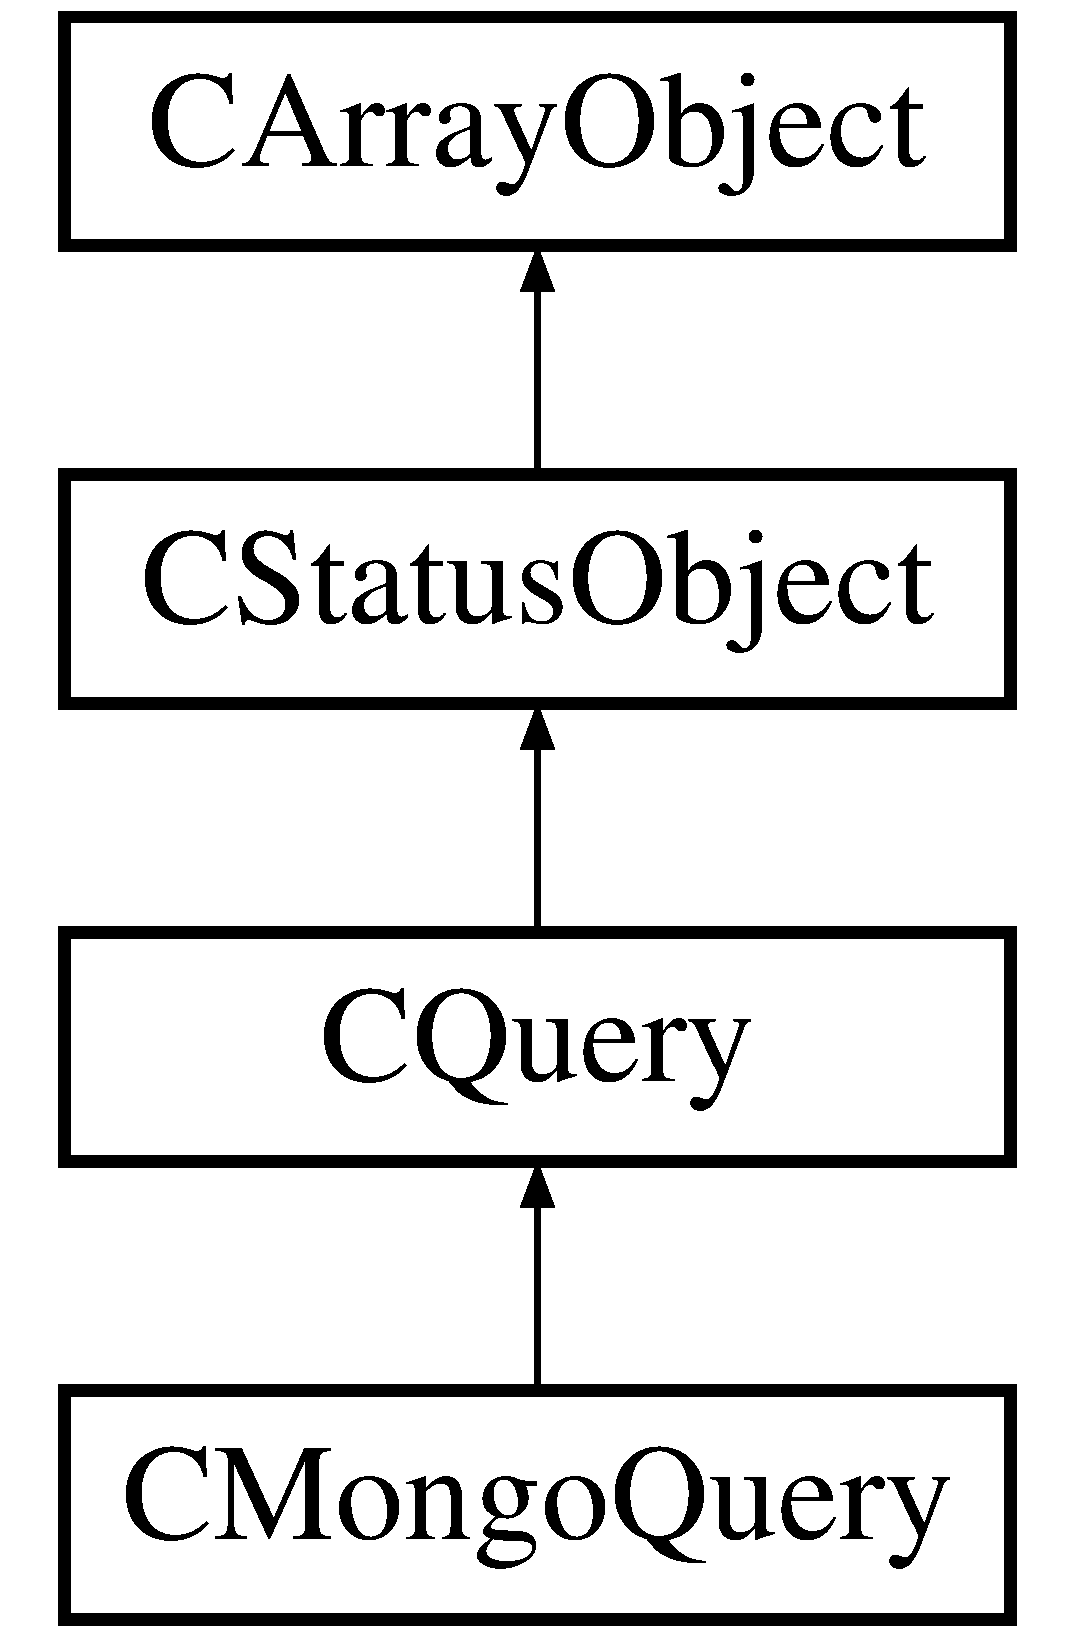
\includegraphics[height=4.000000cm]{class_c_query}
\end{center}
\end{figure}
\subsection*{Public Member Functions}
\begin{DoxyCompactItemize}
\item 
\hyperlink{class_c_query_a5f622c663cffb67955a528cac46502f9}{\-\_\-\-\_\-construct} (\$the\-Query=N\-U\-L\-L)
\item 
\hyperlink{class_c_query_a6cd7ba8e153fc299ba87b614ccb56486}{Append\-Statement} (\$the\-Statement, \$the\-Condition=k\-O\-P\-E\-R\-A\-T\-O\-R\-\_\-\-A\-N\-D)
\item 
\hyperlink{class_c_query_a715ac553707078841213f7b874cbc48e}{Validate} ()
\end{DoxyCompactItemize}
\subsection*{Protected Member Functions}
\begin{DoxyCompactItemize}
\item 
\hyperlink{class_c_query_a1a01d39eedd2951f704dc75c58fb477c}{\-\_\-\-Append\-Statement} (\&\$the\-Query, \$the\-Condition, \$the\-Statement)
\item 
\hyperlink{class_c_query_a5fbde46df4bb30cb252647f0e47cbbde}{\-\_\-\-Validate\-Condition} (\$the\-Condition, \$the\-Statements, \$the\-Level)
\item 
\hyperlink{class_c_query_afe96707c9ed84ee197dae56c9f05f2a4}{\-\_\-\-Validate\-Statement} (\$the\-Statement, \$the\-Level)
\end{DoxyCompactItemize}
\subsection*{Additional Inherited Members}


\subsection{Constructor \& Destructor Documentation}
\hypertarget{class_c_query_a5f622c663cffb67955a528cac46502f9}{\index{C\-Query@{C\-Query}!\-\_\-\-\_\-construct@{\-\_\-\-\_\-construct}}
\index{\-\_\-\-\_\-construct@{\-\_\-\-\_\-construct}!CQuery@{C\-Query}}
\subsubsection[{\-\_\-\-\_\-construct}]{\setlength{\rightskip}{0pt plus 5cm}C\-Query\-::\-\_\-\-\_\-construct (
\begin{DoxyParamCaption}
\item[{}]{\$the\-Query = {\ttfamily NULL}}
\end{DoxyParamCaption}
)}}\label{class_c_query_a5f622c663cffb67955a528cac46502f9}
Instantiate class.

If you omit the parameter the method will instantiate an empty query, if you provide an array or Array\-Object it will assume the structure to be a query and will instantiate the object with it; any other data type will raise an exception.


\begin{DoxyParams}[1]{Parameters}
mixed & {\em \$the\-Query} & Query data.\\
\hline
\end{DoxyParams}
public 

\subsection{Member Function Documentation}
\hypertarget{class_c_query_a1a01d39eedd2951f704dc75c58fb477c}{\index{C\-Query@{C\-Query}!\-\_\-\-Append\-Statement@{\-\_\-\-Append\-Statement}}
\index{\-\_\-\-Append\-Statement@{\-\_\-\-Append\-Statement}!CQuery@{C\-Query}}
\subsubsection[{\-\_\-\-Append\-Statement}]{\setlength{\rightskip}{0pt plus 5cm}C\-Query\-::\-\_\-\-Append\-Statement (
\begin{DoxyParamCaption}
\item[{\&}]{\$the\-Query, }
\item[{}]{\$the\-Condition, }
\item[{}]{\$the\-Statement}
\end{DoxyParamCaption}
)\hspace{0.3cm}{\ttfamily [protected]}}}\label{class_c_query_a1a01d39eedd2951f704dc75c58fb477c}
Append statement.

This method will append the provided statement to the current query.

Statements of the same type, \hyperlink{}{A\-N\-D} and \hyperlink{}{N\-A\-N\-D}, or \hyperlink{}{O\-R} and \hyperlink{}{N\-O\-R}, will be added at the same level. If the top level is an \hyperlink{}{O\-R} or \hyperlink{}{N\-O\-R} and the provided statement is an \hyperlink{}{A\-N\-D} or \hyperlink{}{N\-A\-N\-D}, the latter will be promoted to the top level.

The parameters to this method are\-:


\begin{DoxyItemize}
\item {\bfseries \&\$the\-Query}\-: Query receiving statement. 
\item {\bfseries \$the\-Condition}\-: Statement condition. 
\item {\bfseries \$the\-Condition}\-: Boolean statement condition code. 
\end{DoxyItemize}


\begin{DoxyParams}[1]{Parameters}
reference & {\em \&\$the\-Query} & Query. \\
\hline
array & {\em \$the\-Condition} & Statement condition. \\
\hline
string & {\em \$the\-Statement} & Statement.\\
\hline
\end{DoxyParams}
protected \hypertarget{class_c_query_a5fbde46df4bb30cb252647f0e47cbbde}{\index{C\-Query@{C\-Query}!\-\_\-\-Validate\-Condition@{\-\_\-\-Validate\-Condition}}
\index{\-\_\-\-Validate\-Condition@{\-\_\-\-Validate\-Condition}!CQuery@{C\-Query}}
\subsubsection[{\-\_\-\-Validate\-Condition}]{\setlength{\rightskip}{0pt plus 5cm}C\-Query\-::\-\_\-\-Validate\-Condition (
\begin{DoxyParamCaption}
\item[{}]{\$the\-Condition, }
\item[{}]{\$the\-Statements, }
\item[{}]{\$the\-Level}
\end{DoxyParamCaption}
)\hspace{0.3cm}{\ttfamily [protected]}}}\label{class_c_query_a5fbde46df4bb30cb252647f0e47cbbde}
Validate condition.

This method expects a condition as its argument, it will check if it is a valid condition, then it will \hyperlink{class_c_query_afe96707c9ed84ee197dae56c9f05f2a4}{validate} all condition statements.


\begin{DoxyParams}[1]{Parameters}
string & {\em \$the\-Condition} & Boolean condition. \\
\hline
array & {\em \$the\-Statements} & Statements list. \\
\hline
integer & {\em \$the\-Level} & \mbox{[}P\-R\-I\-V\-A\-T\-E\mbox{]} condition level.\\
\hline
\end{DoxyParams}
protected 

Reimplemented in \hyperlink{class_c_mongo_query_a651af70656cb9894ef1885a711a0c141}{C\-Mongo\-Query}.

\hypertarget{class_c_query_afe96707c9ed84ee197dae56c9f05f2a4}{\index{C\-Query@{C\-Query}!\-\_\-\-Validate\-Statement@{\-\_\-\-Validate\-Statement}}
\index{\-\_\-\-Validate\-Statement@{\-\_\-\-Validate\-Statement}!CQuery@{C\-Query}}
\subsubsection[{\-\_\-\-Validate\-Statement}]{\setlength{\rightskip}{0pt plus 5cm}C\-Query\-::\-\_\-\-Validate\-Statement (
\begin{DoxyParamCaption}
\item[{}]{\$the\-Statement, }
\item[{}]{\$the\-Level}
\end{DoxyParamCaption}
)\hspace{0.3cm}{\ttfamily [protected]}}}\label{class_c_query_afe96707c9ed84ee197dae56c9f05f2a4}
Validate statement.

This method expects a statement as its argument, it will check if it is a valid statement and check if all required elements are there.


\begin{DoxyParams}[1]{Parameters}
array & {\em \$the\-Statement} & Statement. \\
\hline
integer & {\em \$the\-Level} & \mbox{[}P\-R\-I\-V\-A\-T\-E\mbox{]} condition level.\\
\hline
\end{DoxyParams}
protected \hypertarget{class_c_query_a6cd7ba8e153fc299ba87b614ccb56486}{\index{C\-Query@{C\-Query}!Append\-Statement@{Append\-Statement}}
\index{Append\-Statement@{Append\-Statement}!CQuery@{C\-Query}}
\subsubsection[{Append\-Statement}]{\setlength{\rightskip}{0pt plus 5cm}C\-Query\-::\-Append\-Statement (
\begin{DoxyParamCaption}
\item[{}]{\$the\-Statement, }
\item[{}]{\$the\-Condition = {\ttfamily kOPERATOR\-\_\-AND}}
\end{DoxyParamCaption}
)}}\label{class_c_query_a6cd7ba8e153fc299ba87b614ccb56486}
Append statement.

This method will append the provided statement to the query, the second parameter represents the condition.

Appended statements are merged at the condition level\-: if the condition exists at any level, the statement is appended to that condition; if the condition does not exist, it is created. Obviously, \hyperlink{}{A\-N\-D} and \hyperlink{}{N\-A\-N\-D} are treated as equivalent, as well as \hyperlink{}{O\-R} and \hyperlink{}{N\-O\-R}.

If you provide an object derived from \hyperlink{class_c_query}{C\-Query} as the statement, the method will ignore the condition parameter and append the provided query to the current object.


\begin{DoxyParams}[1]{Parameters}
array & {\em \$the\-Statement} & Statement. \\
\hline
string & {\em \$the\-Condition} & Statement condition.\\
\hline
\end{DoxyParams}
public


\begin{DoxyExceptions}{Exceptions}
{\em Exception} & \\
\hline
\end{DoxyExceptions}
\hypertarget{class_c_query_a715ac553707078841213f7b874cbc48e}{\index{C\-Query@{C\-Query}!Validate@{Validate}}
\index{Validate@{Validate}!CQuery@{C\-Query}}
\subsubsection[{Validate}]{\setlength{\rightskip}{0pt plus 5cm}C\-Query\-::\-Validate (
\begin{DoxyParamCaption}
{}
\end{DoxyParamCaption}
)}}\label{class_c_query_a715ac553707078841213f7b874cbc48e}
Validate query.

This method will check whether the query structure is valid.

public


\begin{DoxyExceptions}{Exceptions}
{\em Exception} & \\
\hline
\end{DoxyExceptions}


The documentation for this class was generated from the following file\-:\begin{DoxyCompactItemize}
\item 
/\-Library/\-Web\-Server/\-Library/wrapper/classes/C\-Query.\-php\end{DoxyCompactItemize}

\hypertarget{class_c_status_object}{\section{C\-Status\-Object Class Reference}
\label{class_c_status_object}\index{C\-Status\-Object@{C\-Status\-Object}}
}
Inheritance diagram for C\-Status\-Object\-:\begin{figure}[H]
\begin{center}
\leavevmode
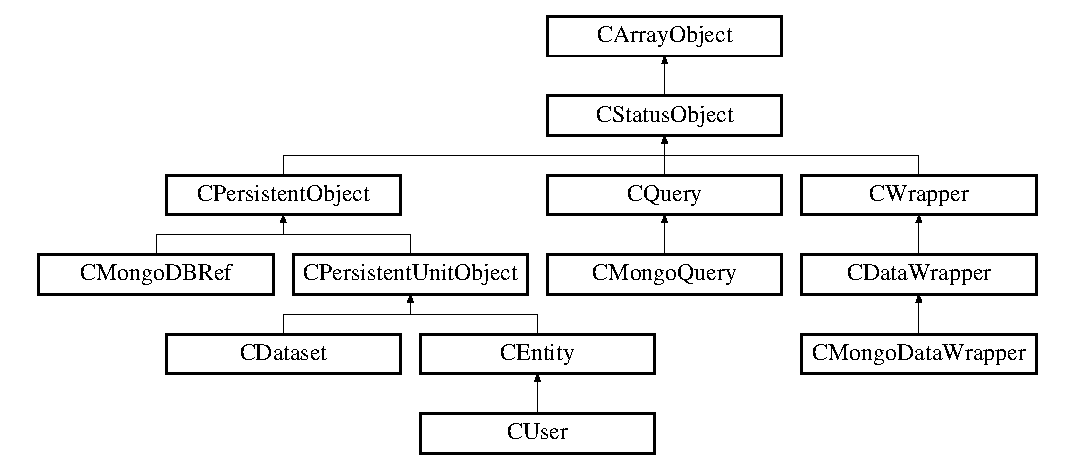
\includegraphics[height=4.000000cm]{class_c_status_object}
\end{center}
\end{figure}
\subsection*{Public Member Functions}
\begin{DoxyCompactItemize}
\item 
\hyperlink{class_c_status_object_a140ef140d4fa1c4a6180e843bd5ec969}{offset\-Set} (\$the\-Offset, \$the\-Value)
\item 
\hyperlink{class_c_status_object_ae733db1bbfffcbe894ea405765ab4150}{offset\-Unset} (\$the\-Offset)
\item 
\hyperlink{class_c_status_object_a6c68cf419c07a3af8ef7e83690590235}{Status} (\$the\-State=N\-U\-L\-L)
\end{DoxyCompactItemize}
\subsection*{Protected Member Functions}
\begin{DoxyCompactItemize}
\item 
\hyperlink{class_c_status_object_a8429102e4f52f7558649b64f4e673a69}{\-\_\-\-Is\-Inited} (\$the\-State=N\-U\-L\-L)
\item 
\hyperlink{class_c_status_object_a19c4ac94dfe26476e780d77b99744d43}{\-\_\-\-Is\-Dirty} (\$the\-State=N\-U\-L\-L)
\item 
\hyperlink{class_c_status_object_a3e37d72a6462d93bf7ff567f07f78093}{\-\_\-\-Manage\-Bit\-Field} (\&\$the\-Field, \$the\-Mask, \$the\-State=N\-U\-L\-L)
\end{DoxyCompactItemize}
\subsection*{Protected Attributes}
\begin{DoxyCompactItemize}
\item 
\hypertarget{class_c_status_object_af80d790146175e2f634d1b84ead1161b}{{\bfseries \$m\-Status} = k\-F\-L\-A\-G\-\_\-\-D\-E\-F\-A\-U\-L\-T}\label{class_c_status_object_af80d790146175e2f634d1b84ead1161b}

\end{DoxyCompactItemize}


\subsection{Member Function Documentation}
\hypertarget{class_c_status_object_a19c4ac94dfe26476e780d77b99744d43}{\index{C\-Status\-Object@{C\-Status\-Object}!\-\_\-\-Is\-Dirty@{\-\_\-\-Is\-Dirty}}
\index{\-\_\-\-Is\-Dirty@{\-\_\-\-Is\-Dirty}!CStatusObject@{C\-Status\-Object}}
\subsubsection[{\-\_\-\-Is\-Dirty}]{\setlength{\rightskip}{0pt plus 5cm}C\-Status\-Object\-::\-\_\-\-Is\-Dirty (
\begin{DoxyParamCaption}
\item[{}]{\$the\-State = {\ttfamily NULL}}
\end{DoxyParamCaption}
)\hspace{0.3cm}{\ttfamily [protected]}}}\label{class_c_status_object_a19c4ac94dfe26476e780d77b99744d43}
Manage dirty status.

This method can be used to get or set the object's dirty state.

A dirty object is one that was modified since the last time this state was probed. In general, this state should be set whenever the persistent properties of the object are modified.

In this class we automatically set this state when \hyperlink{class_c_status_object_a140ef140d4fa1c4a6180e843bd5ec969}{setting} or \hyperlink{class_c_status_object_ae733db1bbfffcbe894ea405765ab4150}{deleting} array store elements.

The method features a single parameter\-:


\begin{DoxyItemize}
\item {\itshape N\-U\-L\-L}\-: The method will return {\itshape T\-R\-U\-E} if the object is dirty, or {\itshape F\-A\-L\-S\-E} if the object is \hyperlink{}{clean}. 
\item {\itshape T\-R\-U\-E}\-: The method will set the object to dirty. 
\item {\itshape F\-A\-L\-S\-E}\-: The method will set the object to \hyperlink{}{clean}. 
\end{DoxyItemize}

In all cases the method will return the state {\itshape after} it was eventually modified.


\begin{DoxyParams}[1]{Parameters}
mixed & {\em \$the\-State} & T\-R\-U\-E, F\-A\-L\-S\-E or N\-U\-L\-L.\\
\hline
\end{DoxyParams}
protected \begin{DoxyReturn}{Returns}
boolean
\end{DoxyReturn}
\hyperlink{class_c_status_object_a3e37d72a6462d93bf7ff567f07f78093}{\-\_\-\-Manage\-Bit\-Field()}

\begin{DoxySeeAlso}{See Also}
k\-F\-L\-A\-G\-\_\-\-S\-T\-A\-T\-E\-\_\-\-D\-I\-R\-T\-Y 
\end{DoxySeeAlso}
\hypertarget{class_c_status_object_a8429102e4f52f7558649b64f4e673a69}{\index{C\-Status\-Object@{C\-Status\-Object}!\-\_\-\-Is\-Inited@{\-\_\-\-Is\-Inited}}
\index{\-\_\-\-Is\-Inited@{\-\_\-\-Is\-Inited}!CStatusObject@{C\-Status\-Object}}
\subsubsection[{\-\_\-\-Is\-Inited}]{\setlength{\rightskip}{0pt plus 5cm}C\-Status\-Object\-::\-\_\-\-Is\-Inited (
\begin{DoxyParamCaption}
\item[{}]{\$the\-State = {\ttfamily NULL}}
\end{DoxyParamCaption}
)\hspace{0.3cm}{\ttfamily [protected]}}}\label{class_c_status_object_a8429102e4f52f7558649b64f4e673a69}
Manage inited status.

This method can be used to get or set the object's inited state.

An object becomes inited when it has all the required elements necessary for it to be correctly used or persistently stored. Such a state indicates that at least the minimum required information was initialised in the object.

The counterpart state indicates that the object still lacks the necessary elements to successfully operate the object.

This method operates by setting or clearing the \hyperlink{}{inited} \hyperlink{class_c_status_object_a6c68cf419c07a3af8ef7e83690590235}{status} flag.

The method features a single parameter\-:


\begin{DoxyItemize}
\item {\itshape N\-U\-L\-L}\-: The method will return {\itshape T\-R\-U\-E} if the object is this state, or {\itshape F\-A\-L\-S\-E} if the object is not in this state. 
\item {\itshape T\-R\-U\-E}\-: The method will set the object to this state. 
\item {\itshape F\-A\-L\-S\-E}\-: The method will reset this state. 
\end{DoxyItemize}

In all cases the method will return the state {\itshape after} it was eventually modified.


\begin{DoxyParams}[1]{Parameters}
mixed & {\em \$the\-State} & T\-R\-U\-E, F\-A\-L\-S\-E or N\-U\-L\-L.\\
\hline
\end{DoxyParams}
protected \begin{DoxyReturn}{Returns}
boolean
\end{DoxyReturn}
\hyperlink{class_c_status_object_a3e37d72a6462d93bf7ff567f07f78093}{\-\_\-\-Manage\-Bit\-Field()}

\begin{DoxySeeAlso}{See Also}
k\-F\-L\-A\-G\-\_\-\-S\-T\-A\-T\-E\-\_\-\-I\-N\-I\-T\-E\-D 
\end{DoxySeeAlso}
\hypertarget{class_c_status_object_a3e37d72a6462d93bf7ff567f07f78093}{\index{C\-Status\-Object@{C\-Status\-Object}!\-\_\-\-Manage\-Bit\-Field@{\-\_\-\-Manage\-Bit\-Field}}
\index{\-\_\-\-Manage\-Bit\-Field@{\-\_\-\-Manage\-Bit\-Field}!CStatusObject@{C\-Status\-Object}}
\subsubsection[{\-\_\-\-Manage\-Bit\-Field}]{\setlength{\rightskip}{0pt plus 5cm}C\-Status\-Object\-::\-\_\-\-Manage\-Bit\-Field (
\begin{DoxyParamCaption}
\item[{\&}]{\$the\-Field, }
\item[{}]{\$the\-Mask, }
\item[{}]{\$the\-State = {\ttfamily NULL}}
\end{DoxyParamCaption}
)\hspace{0.3cm}{\ttfamily [protected]}}}\label{class_c_status_object_a3e37d72a6462d93bf7ff567f07f78093}
Manage bit-\/field property.

This method can be used to manage a bitfield property, it accepts the following parameters\-:


\begin{DoxyItemize}
\item {\bfseries \&\$the\-Field}\-: Reference to the bit-\/field property. 
\item {\bfseries \$the\-Mask}\-: Bit-\/field mask. 
\item {\bfseries \$the\-State}\-: State or operator\-: 
\begin{DoxyItemize}
\item {\itshape N\-U\-L\-L}\-: Return the current value masked by the next parameter. 
\item {\itshape F\-A\-L\-S\-E}\-: Reset the current value using the next parameter as the mask. 
\item {\itshape other}\-: Set the current value to this one, masking the first 31 bits. 
\end{DoxyItemize}
\end{DoxyItemize}

In all cases the method will return the status {\itshape after} it was eventually modified.


\begin{DoxyParams}[1]{Parameters}
reference & {\em \&\$the\-Field} & Bit-\/field reference. \\
\hline
bitfield & {\em \$the\-Mask} & Bit-\/field mask. \\
\hline
mixed & {\em \$the\-State} & Value or operator.\\
\hline
\end{DoxyParams}
protected \begin{DoxyReturn}{Returns}
bitfield
\end{DoxyReturn}
\begin{DoxySeeAlso}{See Also}
k\-F\-L\-A\-G\-\_\-\-D\-E\-F\-A\-U\-L\-T\-\_\-\-M\-A\-S\-K 
\end{DoxySeeAlso}
\hypertarget{class_c_status_object_a140ef140d4fa1c4a6180e843bd5ec969}{\index{C\-Status\-Object@{C\-Status\-Object}!offset\-Set@{offset\-Set}}
\index{offset\-Set@{offset\-Set}!CStatusObject@{C\-Status\-Object}}
\subsubsection[{offset\-Set}]{\setlength{\rightskip}{0pt plus 5cm}C\-Status\-Object\-::offset\-Set (
\begin{DoxyParamCaption}
\item[{}]{\$the\-Offset, }
\item[{}]{\$the\-Value}
\end{DoxyParamCaption}
)}}\label{class_c_status_object_a140ef140d4fa1c4a6180e843bd5ec969}
Set a value for a given offset.

We override this method to handle the \hyperlink{class_c_status_object_a19c4ac94dfe26476e780d77b99744d43}{dirty} \hyperlink{}{flag}\-: on offset value changes we set the state on.


\begin{DoxyParams}[1]{Parameters}
string & {\em \$the\-Offset} & Offset. \\
\hline
string | N\-U\-L\-L & {\em \$the\-Value} & Value to set at offset.\\
\hline
\end{DoxyParams}
public

\hyperlink{class_c_status_object_a19c4ac94dfe26476e780d77b99744d43}{\-\_\-\-Is\-Dirty()}

\begin{DoxySeeAlso}{See Also}
k\-F\-L\-A\-G\-\_\-\-S\-T\-A\-T\-E\-\_\-\-D\-I\-R\-T\-Y 
\end{DoxySeeAlso}


Reimplemented from \hyperlink{class_c_array_object_a41815b543b14d373f68ed34ca53dc9f6}{C\-Array\-Object}.



Reimplemented in \hyperlink{class_c_ontology_term_aba486e72f54e61651a75da75215aaa7c}{C\-Ontology\-Term}, \hyperlink{class_c_dataset_a72f36837282a754ba453799172802e31}{C\-Dataset}, \hyperlink{class_c_wrapper_client_ac37ea353c211b696d11e103a069e8633}{C\-Wrapper\-Client}, \hyperlink{class_c_graph_node_acf4f4240a7807ff16d81378aa282595c}{C\-Graph\-Node}, \hyperlink{class_c_user_aace3446b9cacfe28cc1937c608fcc999}{C\-User}, \hyperlink{class_c_institute_a16c349e22775161c89dbf73850b24cd7}{C\-Institute}, \hyperlink{class_c_f_a_o_institute_ac819c5bfa381ffa0f78b34442d2ea3c2}{C\-F\-A\-O\-Institute}, and \hyperlink{class_c_coded_unit_object_a49bb8f2956cb0551ba827b222778f295}{C\-Coded\-Unit\-Object}.

\hypertarget{class_c_status_object_ae733db1bbfffcbe894ea405765ab4150}{\index{C\-Status\-Object@{C\-Status\-Object}!offset\-Unset@{offset\-Unset}}
\index{offset\-Unset@{offset\-Unset}!CStatusObject@{C\-Status\-Object}}
\subsubsection[{offset\-Unset}]{\setlength{\rightskip}{0pt plus 5cm}C\-Status\-Object\-::offset\-Unset (
\begin{DoxyParamCaption}
\item[{}]{\$the\-Offset}
\end{DoxyParamCaption}
)}}\label{class_c_status_object_ae733db1bbfffcbe894ea405765ab4150}
Reset a value for a given offset.

We override this method to handle the \hyperlink{class_c_status_object_a19c4ac94dfe26476e780d77b99744d43}{dirty} \hyperlink{}{flag}\-: on offset value changes we set the state on.


\begin{DoxyParams}[1]{Parameters}
string & {\em \$the\-Offset} & Offset.\\
\hline
\end{DoxyParams}
public

\hyperlink{class_c_status_object_a19c4ac94dfe26476e780d77b99744d43}{\-\_\-\-Is\-Dirty()}

\begin{DoxySeeAlso}{See Also}
k\-F\-L\-A\-G\-\_\-\-S\-T\-A\-T\-E\-\_\-\-D\-I\-R\-T\-Y 
\end{DoxySeeAlso}


Reimplemented from \hyperlink{class_c_array_object_a2852b78f58379e507b5e7d7cb8e5326b}{C\-Array\-Object}.



Reimplemented in \hyperlink{class_c_ontology_term_a622c31b9466e49a1413d38fda9ef9bb1}{C\-Ontology\-Term}, \hyperlink{class_c_dataset_a9f048a8cbe7109da16a8ef2b7cbd2165}{C\-Dataset}, \hyperlink{class_c_graph_node_aab1d86d6dda1fffa9dd515b23851588a}{C\-Graph\-Node}, \hyperlink{class_c_wrapper_client_af4a349c007923b1229f3099592660d97}{C\-Wrapper\-Client}, \hyperlink{class_c_user_aed8557e18a89d868cedf5a48328b33b2}{C\-User}, \hyperlink{class_c_institute_a8f82ded3b52a6fb609c67e45669e1454}{C\-Institute}, \hyperlink{class_c_f_a_o_institute_a3bd7c59a3da53ba8c3cd1d9d0ff5ae0a}{C\-F\-A\-O\-Institute}, and \hyperlink{class_c_coded_unit_object_a5072e0f72c19260df212a4cf93c9f1cb}{C\-Coded\-Unit\-Object}.

\hypertarget{class_c_status_object_a6c68cf419c07a3af8ef7e83690590235}{\index{C\-Status\-Object@{C\-Status\-Object}!Status@{Status}}
\index{Status@{Status}!CStatusObject@{C\-Status\-Object}}
\subsubsection[{Status}]{\setlength{\rightskip}{0pt plus 5cm}C\-Status\-Object\-::\-Status (
\begin{DoxyParamCaption}
\item[{}]{\$the\-State = {\ttfamily NULL}}
\end{DoxyParamCaption}
)}}\label{class_c_status_object_a6c68cf419c07a3af8ef7e83690590235}
Set or retrieve the object status.

This method can be used to manage the status bitfield as a whole, allowing to set and retrieve the whole set of states.

The parameter can take the following values\-:


\begin{DoxyItemize}
\item {\itshape N\-U\-L\-L}\-: The method will return the current object's states bitfield. 
\item {\itshape F\-A\-L\-S\-E}\-: If this value is passed, the method will reset the object's status by settig it to the \hyperlink{}{default} value. 
\item {\itshape other}\-: In this case the parameter will be interpreted as a 31 bits bit-\/field value and the data member will be replaced with it. 
\end{DoxyItemize}

In all cases the method will return the status {\itshape after} it was eventually modified.


\begin{DoxyParams}[1]{Parameters}
N\-U\-L\-L | F\-A\-L\-S\-E | bitfield & {\em \$the\-State} & N\-U\-L\-L, F\-A\-L\-S\-E or new status.\\
\hline
\end{DoxyParams}
public \begin{DoxyReturn}{Returns}
bitfield
\end{DoxyReturn}
\hyperlink{class_c_status_object_a3e37d72a6462d93bf7ff567f07f78093}{\-\_\-\-Manage\-Bit\-Field()}

\begin{DoxySeeAlso}{See Also}
k\-F\-L\-A\-G\-\_\-\-D\-E\-F\-A\-U\-L\-T\-\_\-\-M\-A\-S\-K 
\end{DoxySeeAlso}


The documentation for this class was generated from the following file\-:\begin{DoxyCompactItemize}
\item 
/\-Library/\-Web\-Server/\-Library/wrapper/classes/C\-Status\-Object.\-php\end{DoxyCompactItemize}

\hypertarget{class_c_user}{\section{C\-User Class Reference}
\label{class_c_user}\index{C\-User@{C\-User}}
}
Inheritance diagram for C\-User\-:\begin{figure}[H]
\begin{center}
\leavevmode
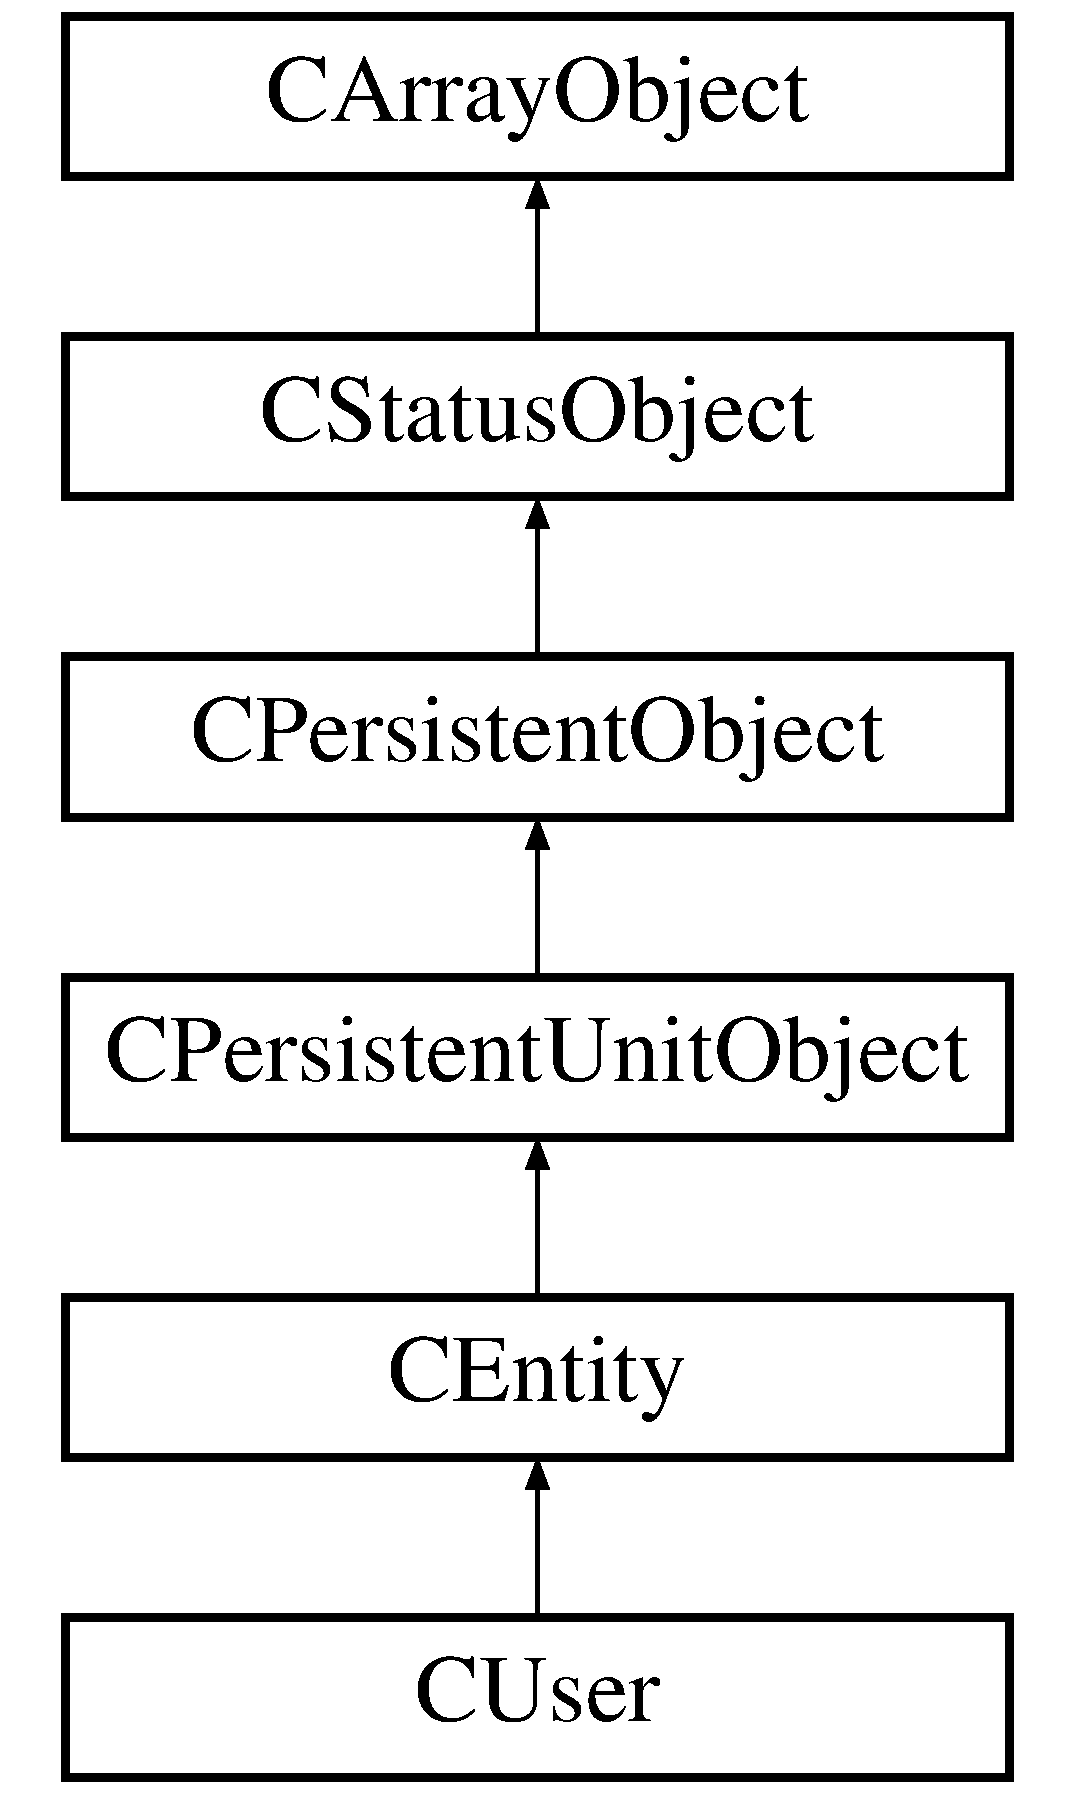
\includegraphics[height=8.000000cm]{class_c_user}
\end{center}
\end{figure}
\subsection*{Public Member Functions}
\begin{DoxyCompactItemize}
\item 
\hyperlink{class_c_user_af83ffccb40893a43d90eafe396cbdec1}{\-\_\-\-\_\-construct} (\$the\-Container=N\-U\-L\-L, \$the\-Identifier=N\-U\-L\-L, \$the\-Modifiers=k\-F\-L\-A\-G\-\_\-\-D\-E\-F\-A\-U\-L\-T)
\item 
\hyperlink{class_c_user_a0e6f1cf51ad23f971ed0999f8d248c8d}{Password} (\$the\-Value=N\-U\-L\-L, \$get\-Old=F\-A\-L\-S\-E)
\item 
\hyperlink{class_c_user_aace3446b9cacfe28cc1937c608fcc999}{offset\-Set} (\$the\-Offset, \$the\-Value)
\item 
\hyperlink{class_c_user_aed8557e18a89d868cedf5a48328b33b2}{offset\-Unset} (\$the\-Offset)
\end{DoxyCompactItemize}
\subsection*{Static Public Member Functions}
\begin{DoxyCompactItemize}
\item 
static \hyperlink{class_c_user_ada20d1f74260a4a5f67453bc9b4f3990}{Hash\-Index} (\$the\-Value)
\end{DoxyCompactItemize}
\subsection*{Protected Member Functions}
\begin{DoxyCompactItemize}
\item 
\hyperlink{class_c_user_aacdc43c5a38cb6b013ee9ce686b186e9}{\-\_\-\-Prepare\-Commit} (\&\$the\-Container, \&\$the\-Identifier, \&\$the\-Modifiers)
\end{DoxyCompactItemize}


\subsection{Constructor \& Destructor Documentation}
\hypertarget{class_c_user_af83ffccb40893a43d90eafe396cbdec1}{\index{C\-User@{C\-User}!\-\_\-\-\_\-construct@{\-\_\-\-\_\-construct}}
\index{\-\_\-\-\_\-construct@{\-\_\-\-\_\-construct}!CUser@{C\-User}}
\subsubsection[{\-\_\-\-\_\-construct}]{\setlength{\rightskip}{0pt plus 5cm}C\-User\-::\-\_\-\-\_\-construct (
\begin{DoxyParamCaption}
\item[{}]{\$the\-Container = {\ttfamily NULL}, }
\item[{}]{\$the\-Identifier = {\ttfamily NULL}, }
\item[{}]{\$the\-Modifiers = {\ttfamily kFLAG\-\_\-DEFAULT}}
\end{DoxyParamCaption}
)}}\label{class_c_user_af83ffccb40893a43d90eafe396cbdec1}
Instantiate class.

We \hyperlink{class_c_coded_unit_object_a314fc62af62314f5ac5acca2ac809900}{overload} the constructor to initialise the \hyperlink{class_c_status_object_a8429102e4f52f7558649b64f4e673a69}{inited} \hyperlink{}{flag} if the \hyperlink{class_c_user_a0e6f1cf51ad23f971ed0999f8d248c8d}{password} element is set.

We also pass the \hyperlink{class_c_persistent_object_aa8dc7db66e2af3d28c2035161a2aabf9}{encoded} \hyperlink{}{flag} to the parent constructor.


\begin{DoxyParams}[1]{Parameters}
mixed & {\em \$the\-Container} & Persistent container. \\
\hline
mixed & {\em \$the\-Identifier} & Object identifier. \\
\hline
bitfield & {\em \$the\-Modifiers} & Create modifiers.\\
\hline
\end{DoxyParams}
public 

Reimplemented from \hyperlink{class_c_coded_unit_object_a314fc62af62314f5ac5acca2ac809900}{C\-Coded\-Unit\-Object}.



\subsection{Member Function Documentation}
\hypertarget{class_c_user_aacdc43c5a38cb6b013ee9ce686b186e9}{\index{C\-User@{C\-User}!\-\_\-\-Prepare\-Commit@{\-\_\-\-Prepare\-Commit}}
\index{\-\_\-\-Prepare\-Commit@{\-\_\-\-Prepare\-Commit}!CUser@{C\-User}}
\subsubsection[{\-\_\-\-Prepare\-Commit}]{\setlength{\rightskip}{0pt plus 5cm}C\-User\-::\-\_\-\-Prepare\-Commit (
\begin{DoxyParamCaption}
\item[{\&}]{\$the\-Container, }
\item[{\&}]{\$the\-Identifier, }
\item[{\&}]{\$the\-Modifiers}
\end{DoxyParamCaption}
)\hspace{0.3cm}{\ttfamily [protected]}}}\label{class_c_user_aacdc43c5a38cb6b013ee9ce686b186e9}
Normalise parameters of a store.

We overload this method to add the \hyperlink{}{k\-E\-N\-T\-I\-T\-Y\-\_\-\-U\-S\-E\-R} \hyperlink{}{type} to the object prior \hyperlink{class_c_persistent_object_a88b1f2b11d3d60e0b3d33d8b0649b68a}{saving} it and we initialise the user \hyperlink{class_c_coded_unit_object_a56af949800e65f9a283239d2e455259f}{code}, if empty, with the \hyperlink{class_c_entity_acf65b6fb2f4195f6c649b4ca506c7899}{e-\/mail}.


\begin{DoxyParams}[1]{Parameters}
reference & {\em \&\$the\-Container} & Object container. \\
\hline
reference & {\em \&\$the\-Identifier} & Object identifier. \\
\hline
reference & {\em \&\$the\-Modifiers} & Commit modifiers.\\
\hline
\end{DoxyParams}
protected


\begin{DoxyExceptions}{Exceptions}
{\em \{@link} & \hyperlink{class_c_exception}{C\-Exception} \hyperlink{class_c_exception}{C\-Exception}\}\\
\hline
\end{DoxyExceptions}
\begin{DoxySeeAlso}{See also}
k\-E\-R\-R\-O\-R\-\_\-\-O\-P\-T\-I\-O\-N\-\_\-\-M\-I\-S\-S\-I\-N\-G 
\end{DoxySeeAlso}


Reimplemented from \hyperlink{class_c_entity_ac306808f0f8404fa405674cbe14fd441}{C\-Entity}.

\hypertarget{class_c_user_ada20d1f74260a4a5f67453bc9b4f3990}{\index{C\-User@{C\-User}!Hash\-Index@{Hash\-Index}}
\index{Hash\-Index@{Hash\-Index}!CUser@{C\-User}}
\subsubsection[{Hash\-Index}]{\setlength{\rightskip}{0pt plus 5cm}static C\-User\-::\-Hash\-Index (
\begin{DoxyParamCaption}
\item[{}]{\$the\-Value}
\end{DoxyParamCaption}
)\hspace{0.3cm}{\ttfamily [static]}}}\label{class_c_user_ada20d1f74260a4a5f67453bc9b4f3990}
Hash index.

This method can be used to format an identifier provided as a string, it will be used by the \hyperlink{class_c_persistent_unit_object_ad1ca0920cf0df3c24351402f9afbf34b}{\-\_\-id} method to format the result of the \hyperlink{class_c_coded_unit_object_a990c19b8bf98d2784da81e3a3121ce56}{\-\_\-index} method. One can consider this as the index hashing method for all derived classes.

In this class we take the provided \hyperlink{class_c_coded_unit_object_a56af949800e65f9a283239d2e455259f}{code} and prefix it with the \hyperlink{}{k\-E\-N\-T\-I\-T\-Y\-\_\-\-U\-S\-E\-R} token, the result will be \hyperlink{class_c_data_type_binary}{hashed}.


\begin{DoxyParams}[1]{Parameters}
string & {\em \$the\-Value} & Value to hash.\\
\hline
\end{DoxyParams}
\begin{DoxyReturn}{Returns}
string 
\end{DoxyReturn}


Reimplemented from \hyperlink{class_c_persistent_unit_object_af0e75c386b883074c8bb677bac500bb3}{C\-Persistent\-Unit\-Object}.

\hypertarget{class_c_user_aace3446b9cacfe28cc1937c608fcc999}{\index{C\-User@{C\-User}!offset\-Set@{offset\-Set}}
\index{offset\-Set@{offset\-Set}!CUser@{C\-User}}
\subsubsection[{offset\-Set}]{\setlength{\rightskip}{0pt plus 5cm}C\-User\-::offset\-Set (
\begin{DoxyParamCaption}
\item[{}]{\$the\-Offset, }
\item[{}]{\$the\-Value}
\end{DoxyParamCaption}
)}}\label{class_c_user_aace3446b9cacfe28cc1937c608fcc999}
Set a value for a given offset.

We overload this method to manage the \hyperlink{class_c_status_object_a8429102e4f52f7558649b64f4e673a69}{inited} \hyperlink{}{status}\-: this is set if the \hyperlink{}{name}, \hyperlink{}{e-\/mail}, \hyperlink{}{password} and the parent \hyperlink{}{code} are set.


\begin{DoxyParams}[1]{Parameters}
string & {\em \$the\-Offset} & Offset. \\
\hline
string | N\-U\-L\-L & {\em \$the\-Value} & Value to set at offset.\\
\hline
\end{DoxyParams}
public

\hyperlink{class_c_status_object_a8429102e4f52f7558649b64f4e673a69}{\-\_\-\-Is\-Inited()}  \hyperlink{class_c_persistent_object_a6520a7bcecf3f39fd61ec6d08f736e77}{\-\_\-\-Is\-Committed()} 

Reimplemented from \hyperlink{class_c_coded_unit_object_a49bb8f2956cb0551ba827b222778f295}{C\-Coded\-Unit\-Object}.

\hypertarget{class_c_user_aed8557e18a89d868cedf5a48328b33b2}{\index{C\-User@{C\-User}!offset\-Unset@{offset\-Unset}}
\index{offset\-Unset@{offset\-Unset}!CUser@{C\-User}}
\subsubsection[{offset\-Unset}]{\setlength{\rightskip}{0pt plus 5cm}C\-User\-::offset\-Unset (
\begin{DoxyParamCaption}
\item[{}]{\$the\-Offset}
\end{DoxyParamCaption}
)}}\label{class_c_user_aed8557e18a89d868cedf5a48328b33b2}
Reset a value for a given offset.

We overload this method to manage the \hyperlink{class_c_status_object_a8429102e4f52f7558649b64f4e673a69}{inited} \hyperlink{}{status}\-: this is set if the \hyperlink{}{name}, \hyperlink{}{e-\/mail}, \hyperlink{}{password} and the parent \hyperlink{}{code} are set.


\begin{DoxyParams}[1]{Parameters}
string & {\em \$the\-Offset} & Offset.\\
\hline
\end{DoxyParams}
public

\hyperlink{class_c_status_object_a8429102e4f52f7558649b64f4e673a69}{\-\_\-\-Is\-Inited()}  \hyperlink{class_c_persistent_object_a6520a7bcecf3f39fd61ec6d08f736e77}{\-\_\-\-Is\-Committed()} 

Reimplemented from \hyperlink{class_c_coded_unit_object_a5072e0f72c19260df212a4cf93c9f1cb}{C\-Coded\-Unit\-Object}.

\hypertarget{class_c_user_a0e6f1cf51ad23f971ed0999f8d248c8d}{\index{C\-User@{C\-User}!Password@{Password}}
\index{Password@{Password}!CUser@{C\-User}}
\subsubsection[{Password}]{\setlength{\rightskip}{0pt plus 5cm}C\-User\-::\-Password (
\begin{DoxyParamCaption}
\item[{}]{\$the\-Value = {\ttfamily NULL}, }
\item[{}]{\$get\-Old = {\ttfamily FALSE}}
\end{DoxyParamCaption}
)}}\label{class_c_user_a0e6f1cf51ad23f971ed0999f8d248c8d}
Manage user password.

This method can be used to manage the user \hyperlink{}{password}, it uses the standard accessor \hyperlink{class_c_attribute_a9d231a47718719fcd6c33f3d0ac91675}{method} to manage the \hyperlink{}{offset}\-:


\begin{DoxyItemize}
\item {\bfseries \$the\-Value}\-: The value or operation\-: 
\begin{DoxyItemize}
\item {\itshape N\-U\-L\-L}\-: Return the current value. 
\item {\itshape F\-A\-L\-S\-E}\-: Delete the value. 
\item {\itshape other}\-: Set value. 
\end{DoxyItemize}
\item {\bfseries \$get\-Old}\-: Determines what the method will return\-: 
\begin{DoxyItemize}
\item {\itshape T\-R\-U\-E}\-: Return the value {\itshape before} it was eventually modified. 
\item {\itshape F\-A\-L\-S\-E}\-: Return the value {\itshape after} it was eventually modified. 
\end{DoxyItemize}
\end{DoxyItemize}


\begin{DoxyParams}[1]{Parameters}
N\-U\-L\-L | F\-A\-L\-S\-E | string & {\em \$the\-Value} & User password or operation. \\
\hline
boolean & {\em \$get\-Old} & T\-R\-U\-E get old value.\\
\hline
\end{DoxyParams}
public \begin{DoxyReturn}{Returns}
string 
\end{DoxyReturn}


The documentation for this class was generated from the following file\-:\begin{DoxyCompactItemize}
\item 
/\-Library/\-Web\-Server/\-Library/wrapper/classes/C\-User.\-php\end{DoxyCompactItemize}

\hypertarget{class_c_wrapper}{\section{C\-Wrapper Class Reference}
\label{class_c_wrapper}\index{C\-Wrapper@{C\-Wrapper}}
}
Inheritance diagram for C\-Wrapper\-:\begin{figure}[H]
\begin{center}
\leavevmode
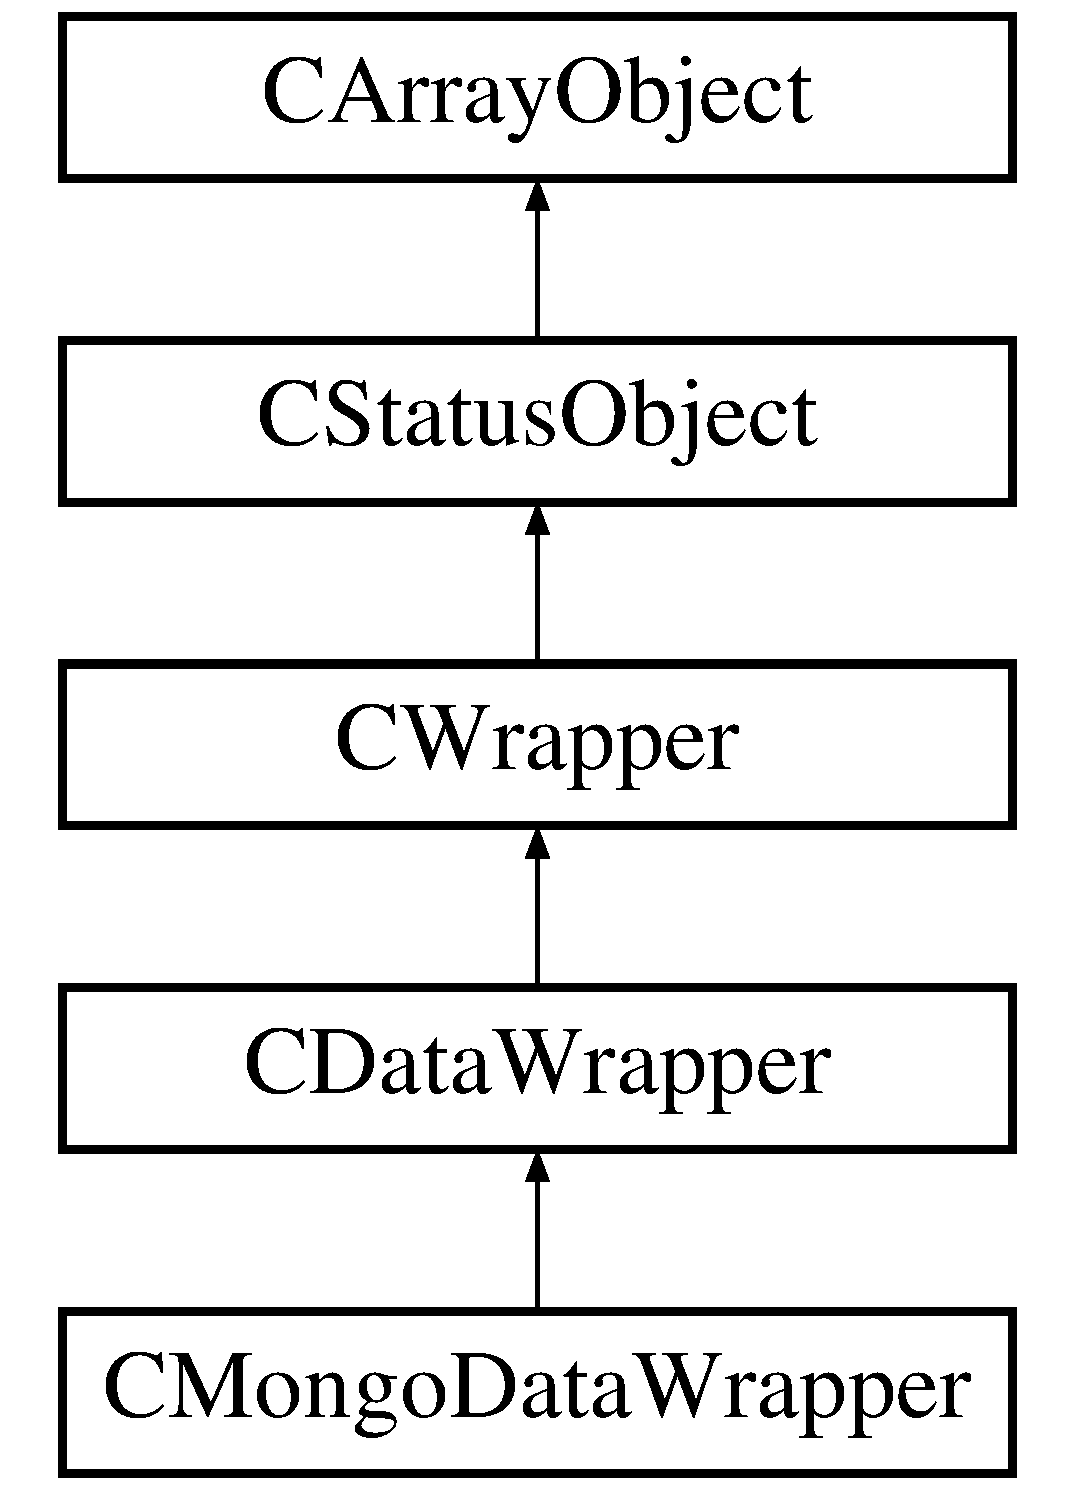
\includegraphics[height=6.000000cm]{class_c_wrapper}
\end{center}
\end{figure}
\subsection*{Public Member Functions}
\begin{DoxyCompactItemize}
\item 
\hyperlink{class_c_wrapper_a683094b01e0682fd34926562d7a052e0}{\-\_\-\-\_\-construct} ()
\item 
\hyperlink{class_c_wrapper_a0e605ca2cdd718ecdeb6f3be9b1f0162}{Handle\-Request} ()
\end{DoxyCompactItemize}
\subsection*{Protected Member Functions}
\begin{DoxyCompactItemize}
\item 
\hyperlink{class_c_wrapper_a8369eec2e53b3f6394a35bcd919d8779}{\-\_\-\-Init\-Status} ()
\item 
\hyperlink{class_c_wrapper_aec2fa3594e36a380d66743b47c24490c}{\-\_\-\-Init\-Options} ()
\item 
\hyperlink{class_c_wrapper_a0e5c5488fce4b388e43dcf6810874d74}{\-\_\-\-Init\-Resources} ()
\item 
\hyperlink{class_c_wrapper_a6675c744053f1b05547ad28fc50a79e6}{\-\_\-\-Parse\-Request} ()
\item 
\hyperlink{class_c_wrapper_a2a3d95961650654468789883ab1607e5}{\-\_\-\-Format\-Request} ()
\item 
\hyperlink{class_c_wrapper_a24b22cfd0022c1cba1741fb294fba5ba}{\-\_\-\-Validate\-Request} ()
\item 
\hyperlink{class_c_wrapper_a53d59f3a61137b8d6f5707d794e2961a}{\-\_\-\-Parse\-Format} ()
\item 
\hyperlink{class_c_wrapper_aa090c135ca1085f46d8cddd393131ea6}{\-\_\-\-Parse\-Operation} ()
\item 
\hyperlink{class_c_wrapper_a13421345af75888b1fa8bcd3381b52a5}{\-\_\-\-Parse\-Timing} ()
\item 
\hyperlink{class_c_wrapper_a8994ff7a5f94438da1c5e3505b145dbd}{\-\_\-\-Validate\-Format} ()
\item 
\hyperlink{class_c_wrapper_aab3f7b2ca4cd9e692c35510d753918a4}{\-\_\-\-Validate\-Operation} ()
\item 
\hyperlink{class_c_wrapper_a12c1dd1f1d1cf0ae889cc19ff17ced0e}{\-\_\-\-Handle\-Request} ()
\item 
\hyperlink{class_c_wrapper_aeff4d2ab12617c1dda2bed705a6969bb}{\-\_\-\-Handle\-\_\-\-List\-Op} (\&\$the\-List)
\item 
\hyperlink{class_c_wrapper_ab58ee7076059e0f992c2a642043b764f}{\-\_\-\-Handle\-\_\-\-Ping} ()
\item 
\hyperlink{class_c_wrapper_aff9eb1799c8f30cb33967c7a50ce6395}{\-\_\-\-Offset\-Manage} (\$the\-Block, \$the\-Element, \$the\-Value=N\-U\-L\-L)
\item 
\hyperlink{class_c_wrapper_ad8dd05c155df0d8fe19be35d4bb67b56}{\-\_\-\-Exception2\-Status} (Exception \$the\-Exception)
\item 
\hyperlink{class_c_wrapper_a60583bacf329d484d01df9851602759f}{\-\_\-\-Encode\-Response} ()
\end{DoxyCompactItemize}
\subsection*{Protected Attributes}
\begin{DoxyCompactItemize}
\item 
\hypertarget{class_c_wrapper_ad9a1a67bf2f21f3b4d0cd83b19be31e3}{{\bfseries \$m\-Received\-Stamp} = N\-U\-L\-L}\label{class_c_wrapper_ad9a1a67bf2f21f3b4d0cd83b19be31e3}

\end{DoxyCompactItemize}


\subsection{Constructor \& Destructor Documentation}
\hypertarget{class_c_wrapper_a683094b01e0682fd34926562d7a052e0}{\index{C\-Wrapper@{C\-Wrapper}!\-\_\-\-\_\-construct@{\-\_\-\-\_\-construct}}
\index{\-\_\-\-\_\-construct@{\-\_\-\-\_\-construct}!CWrapper@{C\-Wrapper}}
\subsubsection[{\-\_\-\-\_\-construct}]{\setlength{\rightskip}{0pt plus 5cm}C\-Wrapper\-::\-\_\-\-\_\-construct (
\begin{DoxyParamCaption}
{}
\end{DoxyParamCaption}
)}}\label{class_c_wrapper_a683094b01e0682fd34926562d7a052e0}
Instantiate class.

The constructor will set-\/up the environment and parse the request. The workflow is as follows\-:


\begin{DoxyItemize}
\item {\itshape Check required elements}\-: The method will check if all required elements of the request are there, only if this is the case will the constructor init the service. 
\item {\itshape Init \hyperlink{class_c_wrapper_a8369eec2e53b3f6394a35bcd919d8779}{status}}\-: The response status will be initialised to the \hyperlink{}{idle} state. 
\item {\itshape Init \hyperlink{class_c_wrapper_aec2fa3594e36a380d66743b47c24490c}{options}}\-: Service options will be initialised. 
\item {\itshape Init \hyperlink{class_c_wrapper_a0e5c5488fce4b388e43dcf6810874d74}{resources}}\-: Eventual resources are initialised. 
\item {\itshape \hyperlink{class_c_wrapper_a6675c744053f1b05547ad28fc50a79e6}{Parse} request}\-: The request is parsed. 
\item {\itshape \hyperlink{class_c_wrapper_a2a3d95961650654468789883ab1607e5}{Format} request}\-: The request is normalised if necessary. 
\item {\itshape \hyperlink{class_c_wrapper_a24b22cfd0022c1cba1741fb294fba5ba}{Validate} request}\-: The request is validated. 
\end{DoxyItemize}

This protected interface should be overloaded by derived classes to implement custom services.

public

\hyperlink{class_c_wrapper_a8369eec2e53b3f6394a35bcd919d8779}{\-\_\-\-Init\-Status()}  \hyperlink{class_c_wrapper_aec2fa3594e36a380d66743b47c24490c}{\-\_\-\-Init\-Options()}  \hyperlink{class_c_wrapper_a0e5c5488fce4b388e43dcf6810874d74}{\-\_\-\-Init\-Resources()}  \hyperlink{class_c_wrapper_a6675c744053f1b05547ad28fc50a79e6}{\-\_\-\-Parse\-Request()}  \hyperlink{class_c_wrapper_a2a3d95961650654468789883ab1607e5}{\-\_\-\-Format\-Request()}  \hyperlink{class_c_wrapper_a24b22cfd0022c1cba1741fb294fba5ba}{\-\_\-\-Validate\-Request()}  \hyperlink{class_c_wrapper_ad8dd05c155df0d8fe19be35d4bb67b56}{\-\_\-\-Exception2\-Status()}  \hyperlink{class_c_wrapper_a60583bacf329d484d01df9851602759f}{\-\_\-\-Encode\-Response()} 

\subsection{Member Function Documentation}
\hypertarget{class_c_wrapper_a60583bacf329d484d01df9851602759f}{\index{C\-Wrapper@{C\-Wrapper}!\-\_\-\-Encode\-Response@{\-\_\-\-Encode\-Response}}
\index{\-\_\-\-Encode\-Response@{\-\_\-\-Encode\-Response}!CWrapper@{C\-Wrapper}}
\subsubsection[{\-\_\-\-Encode\-Response}]{\setlength{\rightskip}{0pt plus 5cm}C\-Wrapper\-::\-\_\-\-Encode\-Response (
\begin{DoxyParamCaption}
{}
\end{DoxyParamCaption}
)\hspace{0.3cm}{\ttfamily [protected]}}}\label{class_c_wrapper_a60583bacf329d484d01df9851602759f}
Encode response.

This method will return the encoded response string.

protected \begin{DoxyReturn}{Returns}
string$|$\-N\-U\-L\-L 
\end{DoxyReturn}
\hypertarget{class_c_wrapper_ad8dd05c155df0d8fe19be35d4bb67b56}{\index{C\-Wrapper@{C\-Wrapper}!\-\_\-\-Exception2\-Status@{\-\_\-\-Exception2\-Status}}
\index{\-\_\-\-Exception2\-Status@{\-\_\-\-Exception2\-Status}!CWrapper@{C\-Wrapper}}
\subsubsection[{\-\_\-\-Exception2\-Status}]{\setlength{\rightskip}{0pt plus 5cm}C\-Wrapper\-::\-\_\-\-Exception2\-Status (
\begin{DoxyParamCaption}
\item[{Exception}]{\$the\-Exception}
\end{DoxyParamCaption}
)\hspace{0.3cm}{\ttfamily [protected]}}}\label{class_c_wrapper_ad8dd05c155df0d8fe19be35d4bb67b56}
Set status from exception.

This method can be used to set the service status according to an exception\-:


\begin{DoxyItemize}
\item {\itshape \hyperlink{class_c_exception_a2bef90da8a35e80dda8072d4f748ec20}{Severity}}\-: This value will be set as the status \hyperlink{}{status}. 
\item {\itshape \hyperlink{}{Code}}\-: This value will be set as the status \hyperlink{}{code}. 
\item {\itshape \hyperlink{}{Message}}\-: This value will be set in the status \hyperlink{}{description} field as a language block. 
\item {\itshape \hyperlink{}{File}}\-: This value will be set in the status \hyperlink{}{annotations}. 
\item {\itshape \hyperlink{}{Line}}\-: This value will be set in the status \hyperlink{}{annotations}. 
\item {\itshape \hyperlink{}{Trace}}\-: This value will be set in the status \hyperlink{}{annotations}. 
\item {\itshape \hyperlink{class_c_exception_abcbd46a262790fcbe3493e30a6418821}{References}}\-: These valuew will be set in the status \hyperlink{}{annotations}. 
\end{DoxyItemize}


\begin{DoxyParams}[1]{Parameters}
Exception & {\em \$the\-Exception} & Exception.\\
\hline
\end{DoxyParams}
protected \hypertarget{class_c_wrapper_a2a3d95961650654468789883ab1607e5}{\index{C\-Wrapper@{C\-Wrapper}!\-\_\-\-Format\-Request@{\-\_\-\-Format\-Request}}
\index{\-\_\-\-Format\-Request@{\-\_\-\-Format\-Request}!CWrapper@{C\-Wrapper}}
\subsubsection[{\-\_\-\-Format\-Request}]{\setlength{\rightskip}{0pt plus 5cm}C\-Wrapper\-::\-\_\-\-Format\-Request (
\begin{DoxyParamCaption}
{}
\end{DoxyParamCaption}
)\hspace{0.3cm}{\ttfamily [protected]}}}\label{class_c_wrapper_a2a3d95961650654468789883ab1607e5}
Format request.

This method should perform any needed formatting before the request will be handled.

In this class we do nothing.

protected 

Reimplemented in \hyperlink{class_c_data_wrapper_ab46c0e9797e8636ca1c9d535b377b90a}{C\-Data\-Wrapper}, \hyperlink{class_c_warehouse_wrapper_a4bd0282949f52ce148b60218c48ddde5}{C\-Warehouse\-Wrapper}, and \hyperlink{class_c_mongo_data_wrapper_abbc0d41394dda4a27eefa8481065749a}{C\-Mongo\-Data\-Wrapper}.

\hypertarget{class_c_wrapper_aeff4d2ab12617c1dda2bed705a6969bb}{\index{C\-Wrapper@{C\-Wrapper}!\-\_\-\-Handle\-\_\-\-List\-Op@{\-\_\-\-Handle\-\_\-\-List\-Op}}
\index{\-\_\-\-Handle\-\_\-\-List\-Op@{\-\_\-\-Handle\-\_\-\-List\-Op}!CWrapper@{C\-Wrapper}}
\subsubsection[{\-\_\-\-Handle\-\_\-\-List\-Op}]{\setlength{\rightskip}{0pt plus 5cm}C\-Wrapper\-::\-\_\-\-Handle\-\_\-\-List\-Op (
\begin{DoxyParamCaption}
\item[{\&}]{\$the\-List}
\end{DoxyParamCaption}
)\hspace{0.3cm}{\ttfamily [protected]}}}\label{class_c_wrapper_aeff4d2ab12617c1dda2bed705a6969bb}
Handle \hyperlink{}{list} operations request.

This method will handle the \hyperlink{}{k\-A\-P\-I\-\_\-\-O\-P\-\_\-\-H\-E\-L\-P} request, which should return the list of supported operations.


\begin{DoxyParams}[1]{Parameters}
reference & {\em \$the\-List} & Receives operations list.\\
\hline
\end{DoxyParams}
protected 

Reimplemented in \hyperlink{class_c_warehouse_wrapper_a9800cf5ca4bb22cd96a94ef542010adf}{C\-Warehouse\-Wrapper}, \hyperlink{class_c_data_wrapper_afc7251c3aad9141599372d6b94904498}{C\-Data\-Wrapper}, and \hyperlink{class_c_mongo_data_wrapper_a1ca51f95510a94bf26e004ef2e8e8d37}{C\-Mongo\-Data\-Wrapper}.

\hypertarget{class_c_wrapper_ab58ee7076059e0f992c2a642043b764f}{\index{C\-Wrapper@{C\-Wrapper}!\-\_\-\-Handle\-\_\-\-Ping@{\-\_\-\-Handle\-\_\-\-Ping}}
\index{\-\_\-\-Handle\-\_\-\-Ping@{\-\_\-\-Handle\-\_\-\-Ping}!CWrapper@{C\-Wrapper}}
\subsubsection[{\-\_\-\-Handle\-\_\-\-Ping}]{\setlength{\rightskip}{0pt plus 5cm}C\-Wrapper\-::\-\_\-\-Handle\-\_\-\-Ping (
\begin{DoxyParamCaption}
{}
\end{DoxyParamCaption}
)\hspace{0.3cm}{\ttfamily [protected]}}}\label{class_c_wrapper_ab58ee7076059e0f992c2a642043b764f}
Handle \hyperlink{}{ping} request.

This method will handle the \hyperlink{}{k\-A\-P\-I\-\_\-\-O\-P\-\_\-\-P\-I\-N\-G} request, which can be used to check if a service is alive.

The ping request will return by default the \hyperlink{}{status} block.

protected \hypertarget{class_c_wrapper_a12c1dd1f1d1cf0ae889cc19ff17ced0e}{\index{C\-Wrapper@{C\-Wrapper}!\-\_\-\-Handle\-Request@{\-\_\-\-Handle\-Request}}
\index{\-\_\-\-Handle\-Request@{\-\_\-\-Handle\-Request}!CWrapper@{C\-Wrapper}}
\subsubsection[{\-\_\-\-Handle\-Request}]{\setlength{\rightskip}{0pt plus 5cm}C\-Wrapper\-::\-\_\-\-Handle\-Request (
\begin{DoxyParamCaption}
{}
\end{DoxyParamCaption}
)\hspace{0.3cm}{\ttfamily [protected]}}}\label{class_c_wrapper_a12c1dd1f1d1cf0ae889cc19ff17ced0e}
Handle request.

This method will handle the request.

protected

\hyperlink{class_c_wrapper_aeff4d2ab12617c1dda2bed705a6969bb}{\-\_\-\-Handle\-\_\-\-List\-Op()}

\begin{DoxySeeAlso}{See Also}
k\-A\-P\-I\-\_\-\-O\-P\-\_\-\-H\-E\-L\-P k\-A\-P\-I\-\_\-\-O\-P\-\_\-\-P\-I\-N\-G 
\end{DoxySeeAlso}


Reimplemented in \hyperlink{class_c_warehouse_wrapper_a4b909b5b4aba967200ff72e3e6924b5e}{C\-Warehouse\-Wrapper}, and \hyperlink{class_c_mongo_data_wrapper_a811af7e7574a459bc56afa3afa99e1a8}{C\-Mongo\-Data\-Wrapper}.

\hypertarget{class_c_wrapper_aec2fa3594e36a380d66743b47c24490c}{\index{C\-Wrapper@{C\-Wrapper}!\-\_\-\-Init\-Options@{\-\_\-\-Init\-Options}}
\index{\-\_\-\-Init\-Options@{\-\_\-\-Init\-Options}!CWrapper@{C\-Wrapper}}
\subsubsection[{\-\_\-\-Init\-Options}]{\setlength{\rightskip}{0pt plus 5cm}C\-Wrapper\-::\-\_\-\-Init\-Options (
\begin{DoxyParamCaption}
{}
\end{DoxyParamCaption}
)\hspace{0.3cm}{\ttfamily [protected]}}}\label{class_c_wrapper_aec2fa3594e36a380d66743b47c24490c}
Initialise options.

This method is responsible for parsing and setting all default and provided options, derived classes should overload this method to handle custom options.

In this class we initialise the \hyperlink{}{request} and \hyperlink{}{timer} sections if required.

protected

\begin{DoxySeeAlso}{See Also}
k\-A\-P\-I\-\_\-\-D\-A\-T\-A\-\_\-\-R\-E\-Q\-U\-E\-S\-T k\-A\-P\-I\-\_\-\-D\-A\-T\-A\-\_\-\-T\-I\-M\-I\-N\-G 
\end{DoxySeeAlso}


Reimplemented in \hyperlink{class_c_data_wrapper_a85c97add738d08f2f2a9958ffbda6c03}{C\-Data\-Wrapper}, and \hyperlink{class_c_warehouse_wrapper_a8dd1de1d5595647b0999ffa6b658c605}{C\-Warehouse\-Wrapper}.

\hypertarget{class_c_wrapper_a0e5c5488fce4b388e43dcf6810874d74}{\index{C\-Wrapper@{C\-Wrapper}!\-\_\-\-Init\-Resources@{\-\_\-\-Init\-Resources}}
\index{\-\_\-\-Init\-Resources@{\-\_\-\-Init\-Resources}!CWrapper@{C\-Wrapper}}
\subsubsection[{\-\_\-\-Init\-Resources}]{\setlength{\rightskip}{0pt plus 5cm}C\-Wrapper\-::\-\_\-\-Init\-Resources (
\begin{DoxyParamCaption}
{}
\end{DoxyParamCaption}
)\hspace{0.3cm}{\ttfamily [protected]}}}\label{class_c_wrapper_a0e5c5488fce4b388e43dcf6810874d74}
Initialise resources.

In derived classes this should be the method that initialises the data store resources, in this class we have no resources.

protected 

Reimplemented in \hyperlink{class_c_mongo_data_wrapper_a33ff97c26b97d00a67f97d41f67ce47b}{C\-Mongo\-Data\-Wrapper}.

\hypertarget{class_c_wrapper_a8369eec2e53b3f6394a35bcd919d8779}{\index{C\-Wrapper@{C\-Wrapper}!\-\_\-\-Init\-Status@{\-\_\-\-Init\-Status}}
\index{\-\_\-\-Init\-Status@{\-\_\-\-Init\-Status}!CWrapper@{C\-Wrapper}}
\subsubsection[{\-\_\-\-Init\-Status}]{\setlength{\rightskip}{0pt plus 5cm}C\-Wrapper\-::\-\_\-\-Init\-Status (
\begin{DoxyParamCaption}
{}
\end{DoxyParamCaption}
)\hspace{0.3cm}{\ttfamily [protected]}}}\label{class_c_wrapper_a8369eec2e53b3f6394a35bcd919d8779}
Initialise status.

This method is responsible for initialising the \hyperlink{}{status} section, derived classes may overload this method if they need to handle other states.

In this class we set the status to \hyperlink{}{idle} and reset the status \hyperlink{}{code}.

protected

\begin{DoxySeeAlso}{See Also}
k\-A\-P\-I\-\_\-\-D\-A\-T\-A\-\_\-\-S\-T\-A\-T\-U\-S 
\end{DoxySeeAlso}
\hypertarget{class_c_wrapper_aff9eb1799c8f30cb33967c7a50ce6395}{\index{C\-Wrapper@{C\-Wrapper}!\-\_\-\-Offset\-Manage@{\-\_\-\-Offset\-Manage}}
\index{\-\_\-\-Offset\-Manage@{\-\_\-\-Offset\-Manage}!CWrapper@{C\-Wrapper}}
\subsubsection[{\-\_\-\-Offset\-Manage}]{\setlength{\rightskip}{0pt plus 5cm}C\-Wrapper\-::\-\_\-\-Offset\-Manage (
\begin{DoxyParamCaption}
\item[{}]{\$the\-Block, }
\item[{}]{\$the\-Element, }
\item[{}]{\$the\-Value = {\ttfamily NULL}}
\end{DoxyParamCaption}
)\hspace{0.3cm}{\ttfamily [protected]}}}\label{class_c_wrapper_aff9eb1799c8f30cb33967c7a50ce6395}
Manage offset.

This method can be used to manage elements within offsets, in other words, it can be used to manage elements within an offset\-:


\begin{DoxyItemize}
\item {\bfseries \$the\-Block}\-: The main offset. 
\item {\bfseries \$the\-Element}\-: The offset within the main offset. 
\item {\bfseries \$the\-Value}\-: The new value or the operation\-: 
\begin{DoxyItemize}
\item {\itshape N\-U\-L\-L}\-: Retrieve the element in the block. 
\item {\itshape F\-A\-L\-S\-E}\-: Delete the element from the block. 
\item {\itshape other}\-: All other data types are interpreted as a new element. 
\end{DoxyItemize}
\end{DoxyItemize}


\begin{DoxyParams}[1]{Parameters}
string & {\em \$the\-Block} & Object block. \\
\hline
string & {\em \$the\-Element} & Object block element. \\
\hline
mixed & {\em \$the\-Value} & Element value.\\
\hline
\end{DoxyParams}
protected \hypertarget{class_c_wrapper_a53d59f3a61137b8d6f5707d794e2961a}{\index{C\-Wrapper@{C\-Wrapper}!\-\_\-\-Parse\-Format@{\-\_\-\-Parse\-Format}}
\index{\-\_\-\-Parse\-Format@{\-\_\-\-Parse\-Format}!CWrapper@{C\-Wrapper}}
\subsubsection[{\-\_\-\-Parse\-Format}]{\setlength{\rightskip}{0pt plus 5cm}C\-Wrapper\-::\-\_\-\-Parse\-Format (
\begin{DoxyParamCaption}
{}
\end{DoxyParamCaption}
)\hspace{0.3cm}{\ttfamily [protected]}}}\label{class_c_wrapper_a53d59f3a61137b8d6f5707d794e2961a}
Parse format.

This method will parse the request format.

protected

\begin{DoxySeeAlso}{See Also}
k\-A\-P\-I\-\_\-\-D\-A\-T\-A\-\_\-\-R\-E\-Q\-U\-E\-S\-T k\-A\-P\-I\-\_\-\-F\-O\-R\-M\-A\-T 
\end{DoxySeeAlso}
\hypertarget{class_c_wrapper_aa090c135ca1085f46d8cddd393131ea6}{\index{C\-Wrapper@{C\-Wrapper}!\-\_\-\-Parse\-Operation@{\-\_\-\-Parse\-Operation}}
\index{\-\_\-\-Parse\-Operation@{\-\_\-\-Parse\-Operation}!CWrapper@{C\-Wrapper}}
\subsubsection[{\-\_\-\-Parse\-Operation}]{\setlength{\rightskip}{0pt plus 5cm}C\-Wrapper\-::\-\_\-\-Parse\-Operation (
\begin{DoxyParamCaption}
{}
\end{DoxyParamCaption}
)\hspace{0.3cm}{\ttfamily [protected]}}}\label{class_c_wrapper_aa090c135ca1085f46d8cddd393131ea6}
Parse operation.

This method will parse the request operation.

protected

\begin{DoxySeeAlso}{See Also}
k\-A\-P\-I\-\_\-\-D\-A\-T\-A\-\_\-\-R\-E\-Q\-U\-E\-S\-T k\-A\-P\-I\-\_\-\-O\-P\-E\-R\-A\-T\-I\-O\-N 
\end{DoxySeeAlso}
\hypertarget{class_c_wrapper_a6675c744053f1b05547ad28fc50a79e6}{\index{C\-Wrapper@{C\-Wrapper}!\-\_\-\-Parse\-Request@{\-\_\-\-Parse\-Request}}
\index{\-\_\-\-Parse\-Request@{\-\_\-\-Parse\-Request}!CWrapper@{C\-Wrapper}}
\subsubsection[{\-\_\-\-Parse\-Request}]{\setlength{\rightskip}{0pt plus 5cm}C\-Wrapper\-::\-\_\-\-Parse\-Request (
\begin{DoxyParamCaption}
{}
\end{DoxyParamCaption}
)\hspace{0.3cm}{\ttfamily [protected]}}}\label{class_c_wrapper_a6675c744053f1b05547ad28fc50a79e6}
Parse request.

This method should be used to parse the request, check the request elements and make any necessary adjustments before the request is \hyperlink{class_c_wrapper_a24b22cfd0022c1cba1741fb294fba5ba}{validated}.

This is also where the relevant request elements will be logged to the relative response sections.

The method is called by the \hyperlink{class_c_wrapper_a683094b01e0682fd34926562d7a052e0}{constructor} and should be overloaded to handle derived classes custom elements.

In this class we handle the \hyperlink{}{format}, \hyperlink{}{operation} and \hyperlink{}{timing} elements.

protected

\hyperlink{class_c_wrapper_a53d59f3a61137b8d6f5707d794e2961a}{\-\_\-\-Parse\-Format()}  \hyperlink{class_c_wrapper_aa090c135ca1085f46d8cddd393131ea6}{\-\_\-\-Parse\-Operation()}  \hyperlink{class_c_wrapper_a13421345af75888b1fa8bcd3381b52a5}{\-\_\-\-Parse\-Timing()} 

Reimplemented in \hyperlink{class_c_data_wrapper_a8b42bd195d9ec6b38ef8e0df3f5dba7a}{C\-Data\-Wrapper}, \hyperlink{class_c_warehouse_wrapper_aab6f377ec08fc5f868a5ad65691964f6}{C\-Warehouse\-Wrapper}, and \hyperlink{class_c_mongo_data_wrapper_a8ac2f23cfc78f3fba6b256718ed2d105}{C\-Mongo\-Data\-Wrapper}.

\hypertarget{class_c_wrapper_a13421345af75888b1fa8bcd3381b52a5}{\index{C\-Wrapper@{C\-Wrapper}!\-\_\-\-Parse\-Timing@{\-\_\-\-Parse\-Timing}}
\index{\-\_\-\-Parse\-Timing@{\-\_\-\-Parse\-Timing}!CWrapper@{C\-Wrapper}}
\subsubsection[{\-\_\-\-Parse\-Timing}]{\setlength{\rightskip}{0pt plus 5cm}C\-Wrapper\-::\-\_\-\-Parse\-Timing (
\begin{DoxyParamCaption}
{}
\end{DoxyParamCaption}
)\hspace{0.3cm}{\ttfamily [protected]}}}\label{class_c_wrapper_a13421345af75888b1fa8bcd3381b52a5}
Parse timing.

This method will parse the request timers.

protected

\begin{DoxySeeAlso}{See Also}
k\-A\-P\-I\-\_\-\-D\-A\-T\-A\-\_\-\-R\-E\-Q\-U\-E\-S\-T k\-A\-P\-I\-\_\-\-R\-E\-Q\-\_\-\-S\-T\-A\-M\-P 
\end{DoxySeeAlso}
\hypertarget{class_c_wrapper_a8994ff7a5f94438da1c5e3505b145dbd}{\index{C\-Wrapper@{C\-Wrapper}!\-\_\-\-Validate\-Format@{\-\_\-\-Validate\-Format}}
\index{\-\_\-\-Validate\-Format@{\-\_\-\-Validate\-Format}!CWrapper@{C\-Wrapper}}
\subsubsection[{\-\_\-\-Validate\-Format}]{\setlength{\rightskip}{0pt plus 5cm}C\-Wrapper\-::\-\_\-\-Validate\-Format (
\begin{DoxyParamCaption}
{}
\end{DoxyParamCaption}
)\hspace{0.3cm}{\ttfamily [protected]}}}\label{class_c_wrapper_a8994ff7a5f94438da1c5e3505b145dbd}
Validate request format.

This method can be used to check whether the provided \hyperlink{}{format} parameter is valid.

protected

\begin{DoxySeeAlso}{See Also}
k\-T\-Y\-P\-E\-\_\-\-P\-H\-P k\-T\-Y\-P\-E\-\_\-\-J\-S\-O\-N 
\end{DoxySeeAlso}
\hypertarget{class_c_wrapper_aab3f7b2ca4cd9e692c35510d753918a4}{\index{C\-Wrapper@{C\-Wrapper}!\-\_\-\-Validate\-Operation@{\-\_\-\-Validate\-Operation}}
\index{\-\_\-\-Validate\-Operation@{\-\_\-\-Validate\-Operation}!CWrapper@{C\-Wrapper}}
\subsubsection[{\-\_\-\-Validate\-Operation}]{\setlength{\rightskip}{0pt plus 5cm}C\-Wrapper\-::\-\_\-\-Validate\-Operation (
\begin{DoxyParamCaption}
{}
\end{DoxyParamCaption}
)\hspace{0.3cm}{\ttfamily [protected]}}}\label{class_c_wrapper_aab3f7b2ca4cd9e692c35510d753918a4}
Validate request operation.

This method can be used to check whether the provided \hyperlink{}{operation} parameter is valid.

protected

\begin{DoxySeeAlso}{See Also}
k\-A\-P\-I\-\_\-\-O\-P\-\_\-\-H\-E\-L\-P k\-A\-P\-I\-\_\-\-O\-P\-\_\-\-P\-I\-N\-G 
\end{DoxySeeAlso}


Reimplemented in \hyperlink{class_c_warehouse_wrapper_ab9506f24cc7dd6b001991f83bd2b5d55}{C\-Warehouse\-Wrapper}, \hyperlink{class_c_data_wrapper_ac25dbab0dc8d55b3b8f0a4027d4549c6}{C\-Data\-Wrapper}, and \hyperlink{class_c_mongo_data_wrapper_a406b81115b5f3957e6d40ee49ae85a13}{C\-Mongo\-Data\-Wrapper}.

\hypertarget{class_c_wrapper_a24b22cfd0022c1cba1741fb294fba5ba}{\index{C\-Wrapper@{C\-Wrapper}!\-\_\-\-Validate\-Request@{\-\_\-\-Validate\-Request}}
\index{\-\_\-\-Validate\-Request@{\-\_\-\-Validate\-Request}!CWrapper@{C\-Wrapper}}
\subsubsection[{\-\_\-\-Validate\-Request}]{\setlength{\rightskip}{0pt plus 5cm}C\-Wrapper\-::\-\_\-\-Validate\-Request (
\begin{DoxyParamCaption}
{}
\end{DoxyParamCaption}
)\hspace{0.3cm}{\ttfamily [protected]}}}\label{class_c_wrapper_a24b22cfd0022c1cba1741fb294fba5ba}
Validate request.

This method should check that the request is valid and that all required parameters have been sent.

In this class we check the \hyperlink{}{format} and \hyperlink{}{operation} codes (their presence is checked by the \hyperlink{class_c_wrapper_a683094b01e0682fd34926562d7a052e0}{constructor}.

protected

\hyperlink{class_c_wrapper_a8994ff7a5f94438da1c5e3505b145dbd}{\-\_\-\-Validate\-Format()}  \hyperlink{class_c_wrapper_aab3f7b2ca4cd9e692c35510d753918a4}{\-\_\-\-Validate\-Operation()} 

Reimplemented in \hyperlink{class_c_data_wrapper_aed059c9ffcb6e988633ba5b28a875b76}{C\-Data\-Wrapper}, \hyperlink{class_c_warehouse_wrapper_a96537df2b42833302fb52de632a8f8f4}{C\-Warehouse\-Wrapper}, and \hyperlink{class_c_mongo_data_wrapper_a3d06376cb588e5c26751bff3f0083ef5}{C\-Mongo\-Data\-Wrapper}.

\hypertarget{class_c_wrapper_a0e605ca2cdd718ecdeb6f3be9b1f0162}{\index{C\-Wrapper@{C\-Wrapper}!Handle\-Request@{Handle\-Request}}
\index{Handle\-Request@{Handle\-Request}!CWrapper@{C\-Wrapper}}
\subsubsection[{Handle\-Request}]{\setlength{\rightskip}{0pt plus 5cm}C\-Wrapper\-::\-Handle\-Request (
\begin{DoxyParamCaption}
{}
\end{DoxyParamCaption}
)}}\label{class_c_wrapper_a0e605ca2cdd718ecdeb6f3be9b1f0162}
Handle the request.

This method will handle the request.

Note that we only run the method if the object is \hyperlink{class_c_status_object_a8429102e4f52f7558649b64f4e673a69}{inited}, if this is not the case, the method will do nothing.

public

\hyperlink{class_c_wrapper_a12c1dd1f1d1cf0ae889cc19ff17ced0e}{\-\_\-\-Handle\-Request()}  \hyperlink{class_c_wrapper_ad8dd05c155df0d8fe19be35d4bb67b56}{\-\_\-\-Exception2\-Status()}  \hyperlink{class_c_wrapper_a60583bacf329d484d01df9851602759f}{\-\_\-\-Encode\-Response()} 

The documentation for this class was generated from the following file\-:\begin{DoxyCompactItemize}
\item 
/\-Library/\-Web\-Server/\-Library/wrapper/classes/C\-Wrapper.\-php\end{DoxyCompactItemize}

\printindex
\end{document}
